% A LaTeX template fitted for a Phd thesis report
% Copyright (C) 2013 Damien Roque
% Author : Damien Roque <damien.roque_AT_isae-supaero.fr>

\documentclass[a4paper,11pt,twoside]{book}
%\documentclass[a4paper,11pt, twoside]{templates/roque-phdthesis-template}

% Include configuration (loading packages, defining the style of the document...)
\usepackage[utf8]{inputenc}
% Encoding and internationalization
\usepackage[T1]{fontenc}
\usepackage{aecompl}
\usepackage[english]{babel} % Comment this line if the document is written in english
\usepackage{csquotes}


% Title page from the University of Toulouse (see doc for further explanations)
\usepackage[ED=AA, Ets=ISAE]{templates/tlsflyleaf}

\title{Sizing and optimisation priorities applied to a Blended Wing-Body with distributed electric ducted fans}
\author{Alessandro SGUEGLIA}
\defencedate{10/12/2019}
\lab{ISAE-Supaero/DCAS \& ONERA/DTIS}
%\cotutelle{Institut de cotutelle}

%% Directeur(s) de thèse
\nboss{2}                                    % Nombre de directeur(s) de thèse
\makesomeone{boss}{1}{Joseph MORLIER}{}{} % Sera affiché en premier
\makesomeone{boss}{2}{Nathalie BARTOLI}{}{}  % Sera affiché en second
%% Referee
\nreferee{2}
\makesomeone{referee}{1}{Dimitri MAVRIS}{}{}
\makesomeone{referee}{2}{Trevor Munro YOUNG}{}{}
%% Jury
\njudge{3}
\makesomeone{judge}{1}{Yves GOURINAT}{President}{ISAE-Supaero}
\makesomeone{judge}{2}{Fabrizio NICOLOSI}{Adjoint professor}{Università di Napoli ``Federico II''}
\makesomeone{judge}{3}{Dimitri MAVRIS}{Professor}{GeorgiaTech}
\makesomeone{judge}{4}{Trevor Munro YOUNG}{Adjoint professor}{University of Limerick}
\makesomeone{judge}{5}{Roelof VOS}{Adjoint professor}{TU Delft}
\makesomeone{judge}{6}{Joseph MORLIER}{Professor}{ISAE-Supaero}
\makesomeone{judge}{7}{Nathalie BARTOLI}{Research Engineer}{ONERA}
\makesomeone{judge}{8}{Christian BES}{Professor}{Université Paul Sabatier}

% Math packages
\usepackage{amsmath,amssymb}
\usepackage{mathrsfs}
\usepackage{amsthm}
\usepackage{a4wide}
\renewcommand{\baselinestretch}{1.05}

%\DeclarePairedDelimiter\abs{\lvert}{\rvert}%
%\DeclarePairedDelimiter\norm{\lVert}{\rVert}%
%
%% Swap the definition of \abs* and \norm*, so that \abs
%% and \norm resizes the size of the brackets, and the 
%% starred version does not.
%\makeatletter
%\let\oldabs\abs
%\def\abs{\@ifstar{\oldabs}{\oldabs*}}

% Graphics and hyperlinks
\usepackage{graphicx}
\usepackage[hyperindex=true]{hyperref}
\hypersetup{%
	colorlinks=true,
	linkcolor=blue,
	citecolor=blue,
	urlcolor=blue}
%\graphicspath{{.}{images/}}
\usepackage{eso-pic}
\usepackage{rotating}
%\usepackage[font=normalsize]{subfig}
\usepackage{subcaption}
\usepackage{tikz}
\usetikzlibrary{shapes,arrows}
\usepackage{pgfplots}
\pgfplotsset{compat=newest}
\pgfplotsset{plot coordinates/math parser=false}
\newlength\figureheight
\newlength\figurewidth

\pgfkeys{/pgf/number format/.cd,
set decimal separator={,\!},
1000 sep={\,},
} % Comment this line if the document is written in english

\usetikzlibrary{plotmarks}
\usepackage{pdfpages}
\usepackage{mdframed}

\usepackage[strict]{changepage}
\newcommand\BackgroundPic{
\put(0,0){
\parbox[b][\paperheight]{\paperwidth}{%
\vfill
\centering
\includegraphics[width=0.9\paperwidth,height=1\paperheight,keepaspectratio]{images/background-eps-converted-to}%
\vfill
}}}

\usepackage{color}
%\definecolor{linkcol}{rgb}{0,0,0} 
%\definecolor{citecol}{rgb}{0,0,0}
\hypersetup{%
	colorlinks=true,
	linkcolor=black,
	citecolor=blue,
	urlcolor=blue}
%\hypersetup
%{
%bookmarksopen=true,
%pdftitle={Mon sujet de thèse complet},
%pdfauthor={Prénom NOM},
%pdfsubject={Rapport de thèse},
%pdfmenubar=true,
%pdfhighlight=/O,
%colorlinks=true,
%pdfpagelayout=SinglePage,
%pdffitwindow=true,
%linkcolor=linkcol,
%citecolor=citecol,
%urlcolor=linkcol
%}

% Headers and footers
\usepackage{fancyhdr}
\pagestyle{fancy}
\fancyfoot{}
\fancyhead[LE,RO]{\bfseries\thepage}
\fancyhead[RE]{\bfseries\nouppercase{\leftmark}}
\fancyhead[LO]{\bfseries\nouppercase{\rightmark}}
\setlength{\headheight}{15pt}


\let\headruleORIG\headrule
\renewcommand{\headrule}{\color{black} \headruleORIG}
\renewcommand{\headrulewidth}{1.0pt}
\usepackage{colortbl}
\arrayrulecolor{black}

%\fancypagestyle{plain}{
%  \fancyhead{}
%  \fancyfoot[C]{\thepage}
%  \renewcommand{\headrulewidth}{0pt}
%}

\usepackage[footnote]{acronym}

% Mini table of content and acronyms
\usepackage[nottoc, notlof, notlot]{tocbibind}
\usepackage[english]{minitoc}
\setcounter{minitocdepth}{3}
\mtcindent=15pt
\setlength{\parskip}{10pt}

\let\minitocORIG\minitoc
\renewcommand{\minitoc}{\minitocORIG \vspace{1.5em}}

\setcounter{secnumdepth}{5}
\setcounter{tocdepth}{2}
\usepackage{silence}
\usepackage{longtable,tabularx}
\usepackage{multirow}
\usepackage{listings}
\usepackage[titletoc]{appendix}

\definecolor{darkgreen}{rgb}{0,0.5,0}
\lstdefinelanguage{XML}
{
	basicstyle=\ttfamily\footnotesize,
	morestring=[b]",
	moredelim=[s][\bfseries\color{blue}]{<}{\ },
	moredelim=[s][\bfseries\color{blue}]{</}{>},
	moredelim=[l][\bfseries\color{blue}]{/>},
	moredelim=[l][\bfseries\color{blue}]{>},
	morecomment=[s]{<?}{?>},
	morecomment=[s]{<!--}{-->},
	commentstyle=\color{darkgreen},
	stringstyle=\color{blue},
	identifierstyle=\color{red}
}

\WarningFilter{minitoc(hints)}{W0023}
\WarningFilter{minitoc(hints)}{W0024}
\WarningFilter{minitoc(hints)}{W0028}
\WarningFilter{minitoc(hints)}{W0030}

\usepackage{siunitx}
\usepackage{algorithmic}
\usepackage{algorithm}

% References formatting
% Bibtex
% \renewcommand*{\backref}[1]{}
% \renewcommand*{\backrefalt}[4]{%
% \ifcase #1 %
% (Non cité.)%
% \or
% (Cité en page~#2.)%
% \else
% (Cité en pages~#2.)%
% \fi}
% \renewcommand*{\backrefsep}{, }
% \renewcommand*{\backreftwosep}{ et~}
% \renewcommand*{\backreflastsep}{ et~}

% BibLatex
%\usepackage[sort]{natbib}
\usepackage[style=alphabetic,backend=bibtex,isbn=false,doi=false,backref=false,url=true,maxbibnames=99]{biblatex}
\addbibresource{biblio.bib}
\inputencoding{utf8}

% Pages succession
%\usepackage{indentfirst}
\makeatletter
\def\cleardoublepage{\clearpage\if@twoside \ifodd\c@page\else%
  \hbox{}%
  \thispagestyle{empty}%
  \newpage%
  \if@twocolumn\hbox{}\newpage\fi\fi\fi}
\makeatother

\newenvironment{vcenterpage}
{\newpage\vspace*{\fill}\thispagestyle{empty}\renewcommand{\headrulewidth}{0pt}}
{\vspace*{\fill}}

%%% Local Variables: 
%%% mode: latex
%%% TeX-master: "../phdthesis"
%%% End: 


% Include user's macros
% Math macros
\newcommand*{\SET}[1]  {\ensuremath{\mathrm{\mathbf{#1}}}}
\newcommand*{\VEC}[1]  {\ensuremath{\boldsymbol{#1}}}
\newcommand*{\MAT}[1]  {\ensuremath{\boldsymbol{#1}}}
\newcommand*{\OP}[1]  {\ensuremath{\boldsymbol{\mathcal{#1}}}}
\newcommand*{\ESP}[1]  {\ensuremath{ \mathbb{E} \left \{#1 \right \}}}
\newcommand*{\ESPENS}[2]  {\ensuremath{ \mathbb{E}_{#1} \left \{#2 \right \}}}
\newcommand*{\NORM}[1]  {\ensuremath{\left\|#1\right\|}}
\newcommand*{\DPR}[2]  {\ensuremath{\left \langle #1,#2 \right \rangle}}
\newcommand*{\FOURIER}[1]  {\ensuremath{\widehat{#1}}}
\newcommand{\eqdef}{\stackrel{\mathrm{def}}{=}}
\newcommand{\argmax}{\operatornamewithlimits{argmax}}
\newcommand{\argmin}{\operatornamewithlimits{argmin}}
\newcommand{\diag}{\operatorname{diag}}
\newcommand{\ud}{\, \mathrm{d}}
\newcommand{\vect}{\mathrm{Vect}}
\newcommand{\sinc}{\mathrm{sinc}}
\newcommand{\esp}{\ensuremath{\mathrm{E}}} % Problème pour les short captions
\newcommand{\hilbert}{\ensuremath{\mathcal{H}}}
\newcommand{\supps}{\ensuremath{\tilde{\mathrm{supp}}}}
\newcommand{\supp}{\ensuremath{\mathrm{supp}}}
\newcommand{\sgn}{\mathrm{sgn}}
\newcommand{\intTT}{\int_{-T}^{T}}
\newcommand{\intT}{\int_{-\frac{T}{2}}^{\frac{T}{2}}}
\newcommand{\intinf}{\int_{-\infty}^{+\infty}}
\newcommand{\iintinf}{\iint_{-\infty}^{+\infty}}
\newcommand{\iintrr}{\iint\limits_{\SET{R}^2}}
\newcommand{\intr}{\int\limits_{\R}}
\newcommand{\Sh}{\ensuremath{\boldsymbol{U}}}
\newcommand{\C}{\ensuremath{\mathbf{C}}}
\newcommand{\R}{\ensuremath{\mathbf{R}}}
\newcommand{\Z}{\ensuremath{\mathbf{Z}}}
\newcommand{\N}{\ensuremath{\mathbf{N}}}
\newcommand{\K}{\ensuremath{\mathbf{K}}}
\newcommand{\reel}{\mathcal{R}}
\newcommand{\imag}{\mathcal{I}}
\newcommand{\cmnr}{c_{m,n}^\reel}
\newcommand{\cmni}{c_{m,n}^\imag}
\newcommand{\cnr}{c_{n}^\reel}
\newcommand{\cni}{c_{n}^\imag}
\newcommand{\tproto}{g}
\newcommand{\rproto}{\check{g}}
\newcommand{\Tproto}{G}
\newcommand{\Rproto}{\check{G}}
\newcommand{\Tpoly}{F}
\newcommand{\Rpoly}{\check{F}}
\newcommand{\estim}{\tilde{c}}
\newcommand{\egal}{\bar{c}}
\newcommand{\bb}{b}
\newcommand{\bbf}{z}
\newcommand{\bbr}{\zeta}
\newcommand{\LR}{\mathcal{L}_2(\R)}
\newcommand{\LRR}{\mathcal{L}_2(\R^2)}
\newcommand{\LZ}{\ell_2(\Z)}
\newcommand{\LZZ}{\ell_2(\Z^2)}
\newcommand{\peigne}{\ensuremath{\Psi}}
\newcommand{\avec}{\qquad \text{avec} \qquad}

% Theorems definition
\newtheoremstyle{break}
  {11pt}{11pt}%
  {\itshape}{}%
  {\bfseries}{}%
  {\newline}{}%
\theoremstyle{break}

\newtheorem{definition}{Définition}[chapter]
\newtheorem{theoreme}{Théorème}[chapter]
\newtheorem{remarque}{Remarque}[chapter]
\newtheorem{propriete}{Propriété}[chapter]
\newtheorem{exemple}{Exemple}[chapter]

% Example of background tag
% \AddToShipoutPicture{%
% \begin{tikzpicture}[remember picture,overlay]
%   \node [rotate=60,scale=10,text opacity=0.1] at (current page.center) {Brouillon};
% \end{tikzpicture}}

% Example of header tag
% \AddToShipoutPicture{%
% \tikzstyle{block} = [draw, thick, color=blue, scale=1.5,rectangle, minimum height=3em, minimum width=6em]
% \begin{tikzpicture}[remember picture,overlay]
%   \node [coordinate] at (current page.north) (accroche) {};
%   \node [block, below of=accroche] {Diffusion restreinte};
% \end{tikzpicture}}

% Another example of header tag
% \AddToShipoutPicture{%
% \tikzstyle{block} = [draw, thick, color=red, scale=1.5,rectangle, minimum height=3em, minimum width=6em]
% \begin{tikzpicture}[remember picture,overlay]
%   \node [coordinate] at (current page.north) (accroche) {};
%   \node [block, below of=accroche] {Confidentiel Défense};
% \end{tikzpicture}}

%%% Local Variables: 
%%% mode: latex
%%% TeX-master: "../phdthesis"
%%% End: 

\begin{document}
% Include the title pages
% (the first is made mandatory by UDG and the second is more traditional)
\makeflyleaf

%%% Local Variables: 
%%% mode: latex
%%% TeX-master: "../phdthesis"
%%% End: 


% Use roman page numbering for non-significant pages
\frontmatter
\pagenumbering{roman}

%% ----------------------------------------------------------------
% The "Quote Page"
\pagestyle{empty}  % No headers or footers for the following pages

\null\vfill
% Now comes the "Quote", written in italics
\textit{``Considerate la vostra semenza: \\ fatti non foste per viver come bruti \\ ma per seguir virtute e canoscenza.''} \newline
\indent \textit{[``Consider well the seed that gave you birth: \\ you were not made to live as brutes, \\ but to follow virtue and knowledge.``]}

\begin{flushright}
\textit{Dante Alighieri} \\
\textit{La Divina Commedia, Inferno, XXVI, 118--120}
\end{flushright}

\vfill\vfill\vfill\vfill\vfill\vfill\null
\clearpage  % Funny Quote page ended, start a new page
%% ----------------------------------------------------------------

% Build the general table of contents
\setcounter{tocdepth}{1}
% Build a per-chapter table of content
\dominitoc
\tableofcontents
%\adjustmtc

%Acknowledgements
%\cleardoublepage
%\phantomsection
%\chapter*{Acknowledgements}

\addcontentsline{toc}{chapter}{Acknowledgements}
\mtcaddchapter  

And so, as every journey, this one comes to an end too. 
A journey started 3 years ago, a morning of january 2017: it is incredible that 3 years have already been passed since then. 
During this time a lot of people supported me: tenth of pages will not be enough to mention all, but I am in duty to thanks some of them in these short lines. 

First of all, special mention to my Ph.D. directors and supervisors: Nathalie Bartoli, Peter Schmollgruber, Emmanuel Benard and Joseph Morlier. 
Without you, this achievement would have never seen an end. 
I hope that you had a great time as I did working with you. 

Thanks to prof. Dimitri Mavris and dr. Trevor Young, who reviewed the work, and to the jury members, who joined the Ph.D. defense: prof. Yves Gourinat, prof. Christian Bes, dr. Roelof Vos, and prof. Fabrizio Nicolosi. 

Thanks to all the colleagues from ONERA, who take part to the Ph.D. with their suggestions and advice: Sebastien Defoort, Michel Ridel, David Donjat, Remi Lafage, Julie Gauvrit-Ledogar, Sylvain Dubreuil. 

Thanks to Serge Bonnet, Marylene Dufort and Guillame Renaud from AIRBUS, for their collaboration in the Chair CEDAR framework. 

Thanks also to prof. Martins and John Jasa for the MDO Lab. at University of Michigan, as well as Justin Gray from NASA Glenn Research Centre and John Hwang from University of California San Diego, for their contribution to the Ph.D., and a special mention to the Formaction Doctorale of ISAE-Supaero who funded the visit at MDO Lab. in 2018. 

My neverending gratitude to the MAE students from ISAE-Supaero I had the honour to supervise: Larissa Cristina e Cunha Lima, Diana Aboub Karhim, Luca Cerquetani, Pablo Rodriguez Otiero, Harleen Kaur, Paolo Traverso, Sesha Chandini. 
Without the work you did in the Blended Wing-Body project, this reseach would have never seen the light. 

And now, let pass to some more personal acknowledgements. 
At the beginning, my intention was to simply write ``to me'', meaning that this achievement was due to myself, but none is so far from reality. 
If I arrived at this point, it is mainly because of my friend, who have always been from my side. 
First, thanks to all the people from ONERA: Morgane Menz, Gabriel Sarazin, Remy Priem, Marie Chiron, Joan Mas Colomer, Julien Marine, Lynda Ait Oubelli. 
You were more than colleagues, you were friends.

To Alessia, who did not hesitate to take a plane to be here with me in this day, you are really special, and you do not stop to show me that, day by day. 

To Nicola and Alex: our friendship last since our childhood, and despite the kilometers that divide us they will never end to stay close with me. 

To my beloved Antonella, one of my favourite people in the world, as a source of unlimited suggestions and comfort.

Last, but absolutely not least, to Sara, who is the demonstration that sometimes sisterhood is a matter of heart and not blood: thank you for have never given up on me, and trusted me even when I did not. 
This is for you. 

Finally, to my parents and my brother: the family is always a sure nest, and they always gave me all the support possible. 

Well now, was that all of them? 
Only one thing is certain, the best is yet to come.

%%% Local Variables: 
%%% mode: latex
%%% TeX-master: "../phdthesis"
%%% End: 


% Abstract
\cleardoublepage
\phantomsection
\begin{vcenterpage}

\addcontentsline{toc}{chapter}{Summary}
\mtcaddchapter  

\noindent\rule[2pt]{\textwidth}{0.5pt}

{\large\textbf{Abstract ---}}
The increase of air traffic in the last decades and its projections pose a key challenge towards the carbon neutral growth objective. 
To cope with this societal goal, there is a need for disruptive air transport aircraft concepts featuring new technologies with low environmental impact. Such future air vehicle relies on the various interactions between systems, disciplines and components. 
This Ph.D. research thus focuses on the development of a methodology dedicated to the exploration and performance evaluation of unconventional configurations using innovative propulsion concepts. 
The use case to be considered is the optimization at conceptual level of a Blended Wing-Body with distributed electric propulsion, a promising concept which combines high aerodynamic performances and benefits from electric propulsion.

The optimization process based on FAST, the ISAE-SUPAERO / ONERA aircraft sizing tool, has been implemented within OpenMDAO, the NASA open-source multidisciplinary analysis and optimization framework.
With the idea of a progressive enhancement of the multidisciplinary design analysis and a better capture of the different effects, the two pioneering elements have been studied separately.
First, the classical process has been revised to take into account the new hybrid powerplant. 
Second, a methodology has been devised to consider a radically new airframe design. Last, a design process featuring both innovative aspects has been developed to investigate a Blended Wing Body concept with distributed electric propulsion.

Regarding the design process, results show that the use of gradients in the optimization procedure speeds up the process against a gradient-free method up to 70\%. 
This is an important gain in time that facilitates designer’s tasks. For the disruptive concept performances, results have been compared to the ones obtained for a conventional A320 type aircraft based on the same top level requirements and technological horizon. 
Overall, the hybrid electric propulsion concept is interesting as it allows zero emissions for Landing/Take-Off operations, improving the environmental footprint of the aircraft: fuel can be saved for missions below a certain range. 
This limitation is associated to the presence of batteries: indeed they introduce indeed a relevant penalty in weight that cannot be countered by benefits of electrification for longer range. 
Additional simulations indicate that a Blended Wing-Body concept based on a turbo-electric only architecture is constantly performing better than the baseline within the limits of the assumptions.


{\large\textbf{Keywords:}}
Aircraft design, Blended Wing-Body, distributed electric propulsion
\\
\noindent\rule[2pt]{\textwidth}{0.5pt}

%\cleardoublepage
%\noindent\rule[2pt]{\textwidth}{0.5pt}
%{\large\textbf{Résumé ---}}
%L'augmentation du trafic aérien au cours des dernières décennies et ses prévisions constituent un défi majeur pour arriver à une croissance neutre en carbone. 
%Pour atteindre cet objectif sociétal, il est nécessaire de définir, en rupture avec les configurations  actuelles, des concepts d'avion de transport intégrant de nouvelles technologies avec au final un impact minimal sur l'environnement. 
%Ces futurs véhicules aériens reposent entre autres sur diverses interactions entre systèmes, disciplines et composants. 
%Aussi, ces travaux de recherche se focalisent sur le développement d'une méthodologie dédiée à l'exploration et à l'évaluation des performances de configurations non conventionnelles utilisant des concepts de propulsion innovants. 
%Le cas d'utilisation à considérer est l'optimisation au niveau conceptuel d'une aile volante à propulsion électrique distribuée, un concept prometteur combinant des performances aérodynamiques élevées et les avantages de la propulsion électrique.
%
%Le processus d'optimisation qui se base sur FAST, l'outil de dimensionnement avion ISAE-SUPAERO/ONERA, a été mis en œuvre dans OpenMDAO, l’environnement d’analyse et d’optimisation multidisciplinaire Open Source de la NASA. 
%Avec l'idée d'une complexité croissante de l'analyse de conception multidisciplinaire et d'une meilleure identification des différents effets, les deux éléments innovants ont été étudiés séparément. 
%Premièrement, le processus classique a été révisé pour tenir compte des systèmes de propulsion hybride. 
%Deuxièmement, une méthode a été appliquée pour estimer  le dimensionnement d’une cellule avion radicalement innovante. 
%Enfin, un processus de conception intégrant ces deux aspects inédits a été mis au point pour étudier un concept d’aile volante à propulsion électrique distribuée.
%
%En ce qui concerne le processus de conception, les résultats montrent que l’utilisation de gradients dans la procédure d’optimisation réduit les temps de calcul par rapport à une méthode sans gradient d’environ 70\%. 
%Ce gain en temps est un avantage important au niveau du processus avant-projet qui facilite les tâches du concepteur. 
%Pour les performances au niveau avion, les résultats ont été comparés à ceux obtenus pour un avion de type A320 classique, fondés sur les mêmes exigences de haut niveau et le même horizon technologique. 
%Globalement, le concept de propulsion électrique hybride est intéressant car il permet des opérations à proximité du sol (atterrissage, décollage) sans émission et d’économiser du carburant pour les missions situées en dessous d’une certaine distance franchissable. 
%Cette limitation est associée à la présence de batteries : elles introduisent en effet une pénalité de masse significative qui ne peut être annulée par les avantages de l'électrification pour de longues distances. 
%Des simulations supplémentaires indiquent qu'un concept d’aile volante fondé sur une architecture uniquement turbo-électrique consomme toujours moins de carburant que l’avion de référence dans les limites des hypothèses prises en compte.
%
%
%{\large\textbf{Mots clés :}}
%Avant-projet des avions, aile volante, propulsion electrique distribuée
%\\
%\noindent\rule[2pt]{\textwidth}{0.5pt}
%
%\vspace{0.5cm}

\end{vcenterpage}

%%% Local Variables: 
%%% mode: latex
%%% TeX-master: "../phdthesis"
%%% End: 


% Include the nomenclature list
\cleardoublepage
\phantomsection
\chapter*{Nomenclature}
\addcontentsline{toc}{chapter}{Nomenclature} 
\mtcaddchapter 
%\addstarredchapter{List of symbols and acronyms}
%\markboth{List of symbols and acronyms}{List of symbols and acronyms}

% Remember to use italic fonts for foreign words
\noindent
\begin{longtable*}{@{}l @{\quad=\quad} p{14.8cm}@{}}
	\multicolumn{2}{@{}l}{\textbf{Symbols}}\\
	$a_\infty$ & Speed of sound \\
	$\alpha$ & Angle of attack or parameter varying between 0 and 1 \\
	$AR$ & Aspect ratio \\
	$b$ & Span \\
	$BPR$ & By-pass ratio \\
	$\bar{c}$ & Mean aerodynamic chord \\
	$\underline{c}\left(\underline{x}\right)$ & Generic design constraint function \\
	$\underline{c}_{CCM}$ & Vector containing the certification specifications \\
	$C_l$ & 2D lift coefficient \\
	$C_L$ & 3D lift coefficient \\
	$C_{L_{\alpha}}$ & Slope of the $C_L-\alpha$ curve \\
	$C_d$ & 2D drag coefficient \\
	$C_D$ & 3D drag coefficient \\
	$C_{D_i}$ & Induced drag coefficient \\
	$C_{D_f}$ & Friction drag coefficient \\
	$C_{D_w}$ & Wave drag coefficient, for transonic regime \\
	$C_m$ & 2D pitching moment coefficient \\
	$C_{M_{ac}}$ & 3D pitching moment coefficient, referred to the aerodynamic center \\
	$C_{M_{cg}}$ & 3D pitching moment coefficient, referred to the center of gravity \\
	$C_H$ & Hinge momentum coefficient \\
	$\delta$ & Power rate \\
	$\delta_e$ & Elevon's deflection angle \\
	$E_c$ & Energy consumption \\
	$E\left[X\right]$ & Statistical average value of a set of values $X$ \\
	$f\left(\underline{x}\right)$ & Generic objective function \\
	FPR & Fan pressure ratio \\
	$g$ & Acceleration of gravity, in SI 9.806~\si{\meter\per\square\second} \\
	$\gamma$ & Climb angle \\
	$\gamma_{\%}$ & Climb rate, in percentage \\
	$\gamma_a$ & Heat coefficient ratio for the air, 1.4 \\
	$\Delta h$ & Total specific enthalpy variation \\
	$\lambda$ & Taper ratio \\
	$\Lambda_{LE}$ & Sweep angle, computed at leading edge \\
	$\Lambda_{TE}$ & Sweep angle, computed at trailing edge \\
	$\Lambda_{25}$ & Sweep angle, computed at 25\% of the chord \\
	$\mu$ & Mean value \\
	$\mathcal{M}$ & Generic numerical solver \\
	$\mathcal{M}_{takeoff}$ & Pitch moment generated at takeoff \\
	$\mathcal{M}_{H}$ & Hinge momentum for the control surface \\
	$N_b$ & Number of batteries \\
	$N_{EM}$ & Number of electric motors \\
	$N_{GT}$ & Number of gas turbine \\
	$N_{pax}$ & Number of passengers \\
	$\mathcal{N}$ & Yaw moment \\
	$m_f$ & Fuel burn \\
	$m_{f_{\max}}$ & Maximum fuel mass that can be stored in the wing \\
	$\dot{m}_f$ & Fuel flow \\
	$m_{L}$ & Maximum landing mass \\
	$m_{TO}$ & Maximum takeoff mass \\
	$m_{e}$ & Operating empty mass \\
	$m_{PL}$ & Payload mass \\
	$m_{PL_{\max}}$ & Maximum payload \\
	$P$ & Power \\
	PSFC & Power specific fuel consumption \\
	$P_{400}$ & Power required at 400~ft \\
	$r_f$ & Fan radius \\
	$\bar{r}_f$ & Fan radius-to-chord ratio \\
	R & Range \\
	$R_g$ & Gas constant, in SI its value is 287~\si{\joule\per\kilogram\per\kelvin} \\
	$\sigma$ & Variance \\
	$\sigma^{*}$ & Coefficient of variation \\
	$s_i$ & First order Sobol index of the parameter $x_i$ \\
	$s_{T_i}$ & Total Sobol index of the parameter $x_i$ \\
	$S$ & Surface \\
	SFC & Specific fuel consumption \\
	SM & Static margin \\
	$SoC$ & State of charge \\
	$t$ & Time \\
	$T$ & Thrust \\
	$\tau$ & Volume \\
	$\left(\frac{t}{c}\right)$ & Thickness-to-chord ratio \\
	$V_\infty$ & Free stream velocity \\
	$w$ & Width \\
	$W$ & Weight \\
	$\underline{x}$ & Design variables vector \\
	$\underline{y}$ & State variables vector \\

	\multicolumn{2}{@{}l}{}\\
	\multicolumn{2}{@{}l}{\textbf{Subscripts}}\\
	$app$ & Approach \\
	$b$ & Battery \\
	$cab$ & Cable \\
	$cb$ & Centerbody \\
	$core$ & Core, also said bus or power management unit PMU \\	
	$cs$ & Cooling system \\
	$g$ & Generator \\
	$EM$ & Electric motor \\
	$fin$ & Final value \\
	$GT$ & Gas turbine \\
	$HT$ & Horizontal tail \\
	$IC$ & Inverter/converter \\
	$\max$ & Maximum value \\
	$out$ & Outer wing \\
	$toc$ & Top of climb \\
	$tod$ & Top of descent \\
	$tr$ & Transition zone \\
	$VT$ & Vertical tail \\
	$w$ & Wing \\
	
	\multicolumn{2}{@{}l}{}\\
	\multicolumn{2}{@{}l}{\textbf{Superscript}}\\
	(0) & Initial value \\
	* & Final value \\
	\emph{t} & Target variable \\
	
\end{longtable*}

%%% Local Variables: 
%%% mode: latex
%%% TeX-master: "../phdthesis"
%%% End: 


% Include the acronyms
\cleardoublepage
\phantomsection
\chapter*{Acronyms}
\addcontentsline{toc}{chapter}{Acronyms} 
\mtcaddchapter 

\begin{acronym}[pppppppppppp] % Specify the longest acronym in order to set the first column width
\acro{AEO}{All Engine Operative}
\acro{BLI}{Boundary Layer Ingestion}
\acro{BWB}{Blended Wing-Body}
\acro{CFD}{Computational Fluid-Dynamics}
\acro{DP}{Distributed Propulsion}
\acro{DEP}{Distributed Electric Propulsion}
\acro{DOC}{Direct Operating Cost}
\acro{EIS}{Entry Into Service}
\acro{ESAR}{Energy Specific Air Range}
\acro{FAST}{Fixed-wing Aircraft Sizing Tool}
\acro{FEM}{Finite Element Model}
\acro{FPR}{Fan pressure ratio}
\acro{HBPR}{High By-Pass Ratio}
\acro{ICE}{Internal Combustion Engine}
\acro{ISAE}{Institut Sup\'{e}rieur de l'A\'{e}ronautique et de l'Espace}
\acro{LAR}{Least Angle Regression}
\acro{LPA}{Large Passenger Aircraft}
\acro{LoD}{Lift over Drag ratio}
\acro{MAC}{Mean Aerodynamic Chord}
\acro{MEA}{More Electric Aircraft}
\acro{MDA}{Multidisciplinary Design Analysis}
\acro{MDF}{Multidisciplinary Feasible}
\acro{MDO}{Muldisciplinary Design Optimisation}
\acro{MDAO}{Multidisciplinary Design Analysis and Optimisation}
\acro{MFW}{Maximum Fuel Weight}
\acro{MLG}{Main Landing Gear}
\acro{MLW}{Maximum Landing Weight}
\acro{MTOW}{Maximum Takeoff Weight}
\acro{MSE}{Mean Square Error}
\acro{MZFW}{Maximum Zero Fuel Weight}
\acro{NASA}{National Aeronautics and Space Administration}
\acro{OAD}{Overall Aircraft Design}
\acro{OCI}{One Core Inoperative}
\acro{OEI}{One Engine Inoperative}
\acro{ONERA}{Office National d'\'{E}tudes et de Recherches A\'{e}rospatiales}
\acro{OWE}{Operating Weight Empty}
\acro{HE}{Hybrid-Electric}
\acro{ICE}{Internal Combustion Engine}
\acro{PCE}{Polynomial Chaos Expansion}
\acro{PMU}{Power Management Unit}
\acro{PFEE}{Payload Fuel Energy Efficiency}
\acro{PL}{Payload}
\acro{PMU}{Power Management Unit}
\acro{RoC}{Rate of Climb}
\acro{SAR}{Specific Air Range}
\acro{SUGAR}{Subsonic Ultra-Green Aircraft}
\acro{TAW}{Tube-and-wing}
\acro{TLAR}{Top Level Aircraft Requirements}
\acro{xDSM}{eXtended Design Structure Matrix}
\acro{XML}{eXtensible Markup Language}

\end{acronym}

% To cite an acronym in the text : \ac{ASK}
% To cite an acronym in the text without footnote : \acs{ASK}

%%% Local Variables: 
%%% mode: latex
%%% TeX-master: "../phdthesis"
%%% End: 

% Build the list of figures
\cleardoublepage
\phantomsection
%\chapter*{List of figures}
\addcontentsline{toc}{chapter}{List of figures} 
 
\listoffigures
\mtcaddchapter
%\adjustmtc

% Build the list of tables
\cleardoublepage
\phantomsection
%\chapter*{List of tables}
\addcontentsline{toc}{chapter}{List of tables} 

\listoftables 
\mtcaddchapter 
%\adjustmtc

%%%%%%%%%%%%%%%%%%%%%%%%%%
%%% Chapters are included here %%%
%%%%%%%%%%%%%%%%%%%%%%%%%%

% Use arabic page numbering for significant pages
\mainmatter
\pagestyle{fancy}

% Include the chapters
%Introduction
\chapter*{Introduction}
\markboth{Introduction}{Introduction}
\addcontentsline{toc}{chapter}{Introduction}  
\mtcaddchapter 

Since its birth in '30s, air transport sector has been continuously growing each year. 
In last decade, thanks to the entry of new commercial area, such as south America or western Asia, the trend has become exponential. 
According to perspective from Boeing and Airbus, the two main leaders in the sector, the number of aircraft flying will be increased of about 39000+ units in 20.

This growth poses a key problem when looking at the emission level.
According to 2015 data, aviation accounts for the 3\% of total CO\textsubscript{x} and NO\textsubscript{x} emissions.
Without any action taken, predictions indicate that this percentage will reach values between 30 and 50\% in a 20 years horizon. 
To avoid such scenario, a sustainable growth must be found. 

Several consortium and agency, spreaded between America and Europe, have published their objectives for emission reduction in near and long term, up to 2050 horizon. 
All these perspectives are very aggressive, and it is commonly recognised that they cannot been achieved through the incremental approach that has been used so far in aviation. 
The classical ``tube-and-wing'' (TAW) configuration has been indeed developed for more than 70 years, and it offers only small potential gains: it is then necessary to introduce a new paradigm in aircraft design, a disruptive concept, based on innovative technologies, to drastically reduce emission. 
The study of a disruptive concept takes place at conceptual design level, where different configurations are defined and sized in order to downselect the most promising ones for further developments. 
Thus thus Ph.D. proposes to develop a Multidisciplinary Design and Optimisation (MDAO) process tailored to the design of an unconventional configuration that would match stringent environmental goals. 

In literature, two main areas of research have been considered: technologies at airframe level, focusing on more aerodynamically efficient architectures, and technologies at propulsive level, deploying hybrid and electric propulsive chain. 
Given the objectives, a most likely viable aircraft must benefit from a combination of both technologies, leading to an optilised overall configuration including hybrid powerplant. 
The main problem when dealing with such innovative concepts concerns the models: the classical methods proposed by aircraft design handbooks are well suited for a conventional configuration, but lose their validity when the concept is drastically different, as in the case of hybrid propulsion or integrated airframe concepts. 
From this consideration the main problem to be solved can be stated as following: \textbf{``How can unconventional configurations be investigated at conceptual design level''?}
This dissertation proposes an answer to this question in 4 steps.

Chapter~\ref{chap1:state_art} reviews the state of the art, focusing on the works of major interest for this research. 
After a brief introduction to better frame the environmental context, the conceptual aircraft design procedure is presented.
Then, innovative key technologies are explored: one of the most promising technology found in literature is the electric and hybrid propulsion. 
This technology, which has been applied at automotive industry and on some general aviation aircraft, enables a total or partial mission electrification, greening the air and the reduction of emission. 
Also, such propulsion concepts enable the increase of propulsive and aerodynamic efficiency, through distribution of thrust and/or boundary layer ingestion.. 
Both these aspects will be detailed. 
At airframe level, the Blended Wing-Body (BWB) is identified as a promising concept with high aerodynamic efficiency. 
At the end of the review, a promising integrated concept is identified in the Blended Wing-Body (BWB) with distributed electric propulsion.
Following the statement of the research problem, it is found that aircraft design must go towards a Multidisciplinary Design Optimisation approach, since it provides the necessary tools to establish a tradeoff for unconventional configuration, without neglecting any of the possible key interactions. 

Chapter~\ref{chap2:fast_base_mdo} presents the development of an aircraft optimisation sizing platform, based on the integration of the code FAST within OpenMDAO. 
FAST, which stands for Fixed-wing Aircraft Sizing Tool, is a code developed at ONERA and ISAE-Supaero for the preliminary design of large passenger aircraft. 
OpenMDAO, instead, is a MDAO platform, developed at NASA Glenn Research Center, which has been used for a large variety of MDO problems in aeronautics.
After a presentation of both tools, with features and drawbacks, the integration of FAST and OpenMDAO is desribed.
A suitable MDO architecture for aircraft design problem is identified, and the processus carried out in the integration is detailed.
The developed code is used for the optimisation of the Airbus A320 test case, so that gains of the optimisation process would be highlighted.
Subsequently, the code has been used to define a set of reference aircraft, considering entry into service 2035. 
Results will be used later to evaluate performance of the proposed disruptive concept. 

The BWB with distributed electric propulsion concept is based on the integration of two different innovative technologies: a new hybrid powerplant at propulsive level and a non conventional architecture at airframe level. 
To better quantify the impact of each of these aspects on the overall design, they are individually treated considering a conventional tube-and-wing aircraft featuring distributed electric propulsion and a BWB mouting conventional air-breathing engines. 
The coupling between the two finally leads to the proposed concept of BWB with distributed electric propulsion. 
The following two chapters reflects this approach.

Chapter~\ref{chap3:hybrid_dep_exploration} is dedicated to the methodology and the exploration of the first concept, tube-and-wing aircraft with distributed electric propulsion. 
The first part of the chapter focuses on the the methodology: the overall propulsive chain is defined at system level, and then models related to each electric component are presented. 
Afterwards, these models are integrated within the conceptual design loop and required modifications to the disciplines are detailed.  
Finally, the revised sizing process is included in the MDO formulation defined in Chapter~\ref{chap2:fast_base_mdo}, to finally converge towards an optimisation sizing framework for an hybrid aircraft. 
The second part of the chapter presents the sizing results for this concept: at first only the sizing loop is applied, to assess its quality in dealing with the innovative powerplant.
Afterwards, optimisation results are presented, varying also the number of engines, in order to establish a possible tradeoff. 
Aircraft performances are evaluated against the reference aircraft, defined in Chapter~\ref{chap2:fast_base_mdo}. 
A Pareto frontier is also generated, comparing two different optimisation algorithms, one gradient-based and another one gradient-free, in order to assess the reduction in computational cost due to the utilisation of derivatives in the optimisation process. 

Chapter~\ref{chap4:bwb_exploration} presents the methods that have been implemented for the Blended Wing-Body sizing. 
First, the research strategy is detailed: in order to tackle the lack of reference data for the BWB architecture, a multi-fidelity analysis is carried out at disciplinary level, so that fast but reliable methods can be identified and used in the conceptual design stage. 
Once more, revised models are integrated within the sizing loop, and the resulting procedure is included in the MDO formulation. 
Finally have a MDAO framework tailored to BWB with DEP is obtained. 
The first part of the results relates only to application of the sizing loop, considering conventional engines, in order to assess the benefits coming solely from the BWB architecture. 
Afterwards, the powerplant modeled in Chapter~\ref{chap3:hybrid_dep_exploration} is combined with this architecture, and the BWB with distributed electric propulsion is explored. 
In this case too, performances are evaluated against the reference aircraft EIS 2035. 
A Pareto frontier is also obtained, to establish tradeoff for the proposed disruptive concept. 

This dissertation is concluded with an overall revision of the work and possible further development to be made on the Multidisciplinary Design Analysis and Optimisation process. 
%1-State of the art
\chapter{Advanced aircraft design process: a technology review}
\markboth{Advanced aircraft design process: a technology review}{Advanced aircraft design process: a technology review}
\label{chap1:state_art}

%\begin{mdframed}[hidealllines=true,backgroundcolor=lightgray!20]
%	\section*{Résumé}
%	Ce chapitre est le premier de cette thèse et a l’objectif de présenter des notions introductives au problème.
%	Le contexte de cette recherche est lié aux défis de l’aviation pour les années à venir: la réduction des émissions est en effet un des enjeux  des clés grands sociétaux. 
%	En particulier, selon les perspectives données par Boeing et Airbus, ces deux principaux constructeurs aéronautiques estiment que plus de 20 000 appareils voleront dans les 20 prochaines années, dans le segment des courtes et moyennes distances, ce qui deviendra alors le facteur décisif pour répondre aux objectifs environnementaux.
%	Malheureusement, ces objectifs peuvent difficilement être atteints avec une configuration conventionnelle (tube-and-wing), car celle-ci est développée depuis plus de 70 ans et offre encore de faibles gains potentiels. Ainsi, un concept de rupture doit être introduit, au niveau de la conception, afin de trouver une solution prometteuse pour réduire l’empreinte environnementale de l’aviation.
%	
%	Pour mieux cerner le problème, la boucle de conception conceptuelle utilisée jusqu’à présent est détaillée.
%	Ensuite, les technologies innovantes clés étudiées au cours des dernières années sont explorées. 
%	L'innovation peut être principalement apportée à deux niveaux: modification de la cellule (géométrie) ou modification du système propulsif. En ce qui concerne la dernière catégorie, la propulsion hybride/électrique a suscité beaucoup d'intérêt: elle a été appliquée avec succès dans l’industrie automobile et les avions de petite taille et, au cours des prochaines années, différentes organisations souhaitent étendre son application au cas des avions de grande capacité. 
%	La principale caractéristique de la propulsion hybride/électrique est qu’elle permet aux nouveaux appareils de tirer parti de l’intégration entre propulsion et aérodynamique. Par exemple dans un système qui considère la propulsion électrique distribuée conjointement avec un dispositif d’ingestion de couche limite (BLI),  les effets provenant du souffle et du flux ingérant sont renforcés.
%	La discussion va plus loin: dans plusieurs ouvrages, il a été souligné que la BLI fonctionnait mieux pour des grandes cordes, ce qui met l’accent sur la recherche de l’architecture la plus appropriée pour l’intégration d’un tel système. 
%	La réponse est donnée par l’aile volante, qui intègre la charge utile et la structure et offre à la fois de grandes surfaces et un volume important pour l’attribution de sous-systèmes; de plus, elle est naturellement très efficace d’un point de vue aérodynamique.
%	
%	Sur la base de ces considérations, il a été décidé d'étudier comme configuration l’aile volante à propulsion électrique distribuée. 
%	En effet, ce concept a déjà été étudié par la NASA dans le cadre de son programme N3-X, mais leurs travaux portent principalement sur la modélisation des différentes disciplines impliquées. 
%	Dans cette recherche, l'objectif est plutôt de mettre en place une procédure pour son étude au niveau conceptuel, avec une entrée en service prévue en 2035.  
%	La question qui guide cette recherche peut être formulée comme suit: ``Comment le processus de conception avion peut-il être modifié pour l’étude d’une configuration non conventionnelle dotée d’un groupe électrogène hybride innovant?''
%	La réponse peut être exprimée en trois points:
%	\begin{itemize}
%		\item La définition de nouveaux modèles afin de prendre en compte l'impact de l'architecture innovante sur la géométrie, la structure, l'aérodynamique et l'évaluation des performances;
%		
%		\item L’application d’une approche multifidélité pour calibrer les méthodes de conception du niveau conceptuel avec des simulations plus précises;
%		
%		\item La définition d'une procédure de dimensionnement basée sur l'optimisation multidisciplinaire, en raison de sa capacité à établir un compromis tenant compte de toutes les interactions entre les disciplines, particulièrement pertinente pour les aéronefs non conventionnels.
%	\end{itemize}
%	Il est à noter que le cas test considéré introduit deux innovations clés: une au niveau de la cellule (architecture aile volante) et une autre au niveau de la propulsion (utilisation de la propulsion hybride). 
%	Afin de mieux évaluer les avantages découlant de chacun de ces deux aspects, ils ont été étudiés séparément: un aéronef conventionnel à propulsion électrique répartie est d'abord pris en compte, puis un concept d'aile volante équipé de moteurs classiques. La procédure finale provient de l'intégration de ces deux études.
%\end{mdframed}
%
%\cleardoublepage

\minitoc

\clearpage

\begin{mdframed}[hidealllines=true,backgroundcolor=purple!20]
	\section*{Outline}
	
	\begin{itemize}
		\item Aviation challenges for upcoming years are identified, specifically about the problem of emission reduction. 
		
		\item The aircraft conceptual design loop is described. 
		
		\item Different solutions to match the aviation's enviromental goals are explored, to converge towards a promising disruptive concept. 
		
		\item Research problem is stated. 
		
	\end{itemize}
\end{mdframed}

\cleardoublepage

\section{The environmental context}
\label{sec:chap1_context}
In last decades world is facing with a more and more relevant environmental crisis~\cite{bib:nasa_armd, bib:environmental_outlook_2050, bib:he_aviation_course}: CO\textsubscript{2} emission are increasing year by year, and a drastic reduction of these emissions in the upcoming years is a duty, for human sustainability. 

On this scenario, aviation plays a key role too. 
Altough its environmental footprint counts for about 2\%~\cite{bib:iata}, the increasing number of aircraft flying every day, which is doubled in 15 years~\cite{bib:airbus_global_market}, plus the more accessibility to this conveyance, make the trend growing exponentially, as shown in Fig.~\ref{fig:aviation_impact_2050}. 
\begin{figure}[!h]
	\centering
	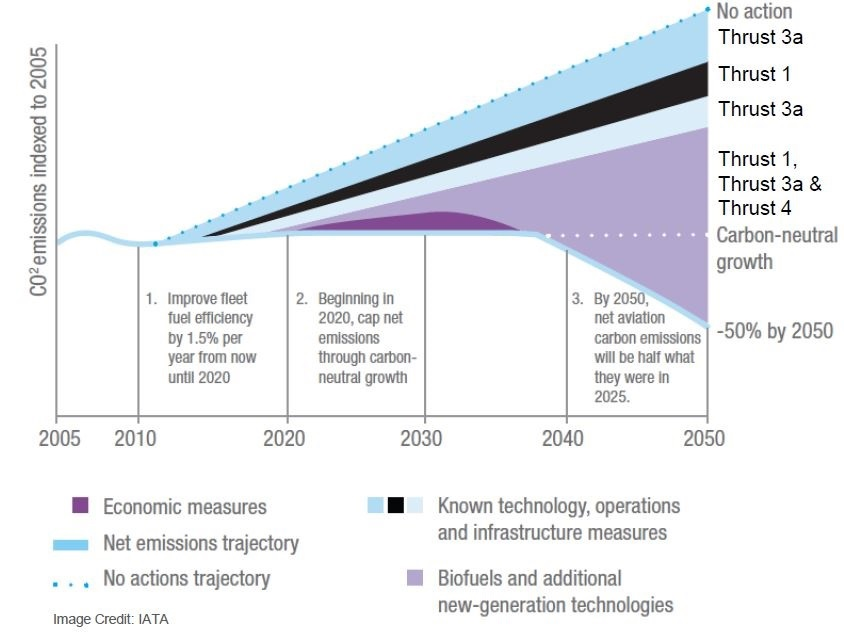
\includegraphics[keepaspectratio, width=0.6\textwidth]{images/chap1/aviation_impact_2050_perspectives.jpg}
	\caption{Aviation environmental footprint perspectives according to NASA ARMD Strategic Thrust~\cite{bib:nasa_armd}.}
	\label{fig:aviation_impact_2050}
\end{figure} 
The image, taken from the NASA ARMD Strategic Thrust~\cite{bib:nasa_armd}, shows the aviation impact perspectives in different scenarios. 
Without any action, its contribution to global emission will be soon unsustainable; the best target is to reduce CO\textsubscript{2} release up to 50\%, to maintain a sustainable level. 
The 50\% reduction goal is shared by other associations and projects in Europe too: both ATAG~\cite{bib:atag} and ACARE~\cite{bib:acare} presented their objectives, in line with the NASA studies.

According to a study, conducted by Boeing, the most critic segment is the one of large passenger aircraft (single and twin aisle)~\cite{bib:he_aviation_course}: their contribution is estimated to be around 93\%, as shown in the breakdown of Fig.~\ref{fig:aviation_emission_breakdown}.
Nowadays, with current electric technology, small regional aircraft are already being electrified, but from this analysis it is clear that the major efforts in next years will be to go on large passenger aircraft. 
\begin{figure}[!h]
	\centering
	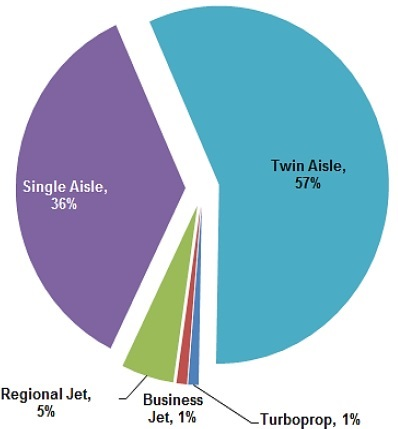
\includegraphics[keepaspectratio, width=0.4\textwidth]{images/chap1/co2_emission_breakdown.jpg}
	\caption{Percentage of CO\textsubscript{2} emission per type of aircraft~\cite{bib:he_aviation_course}.}
	\label{fig:aviation_emission_breakdown}
\end{figure} 

Besides the emissions, which remain the most important issue, also the noise and the energy consumption are relevant aspects to be reduced. 
All the goals can be summed up with a technological table, an example is given in Table~\ref{tab:nasa_armd_table}, where the short, mid and long term goals are well identified.
These are the objectives of NASA N+3 project~\cite{bib:follen_nasa_np3}, started in 2011 and still on-going: despite they seems to be very aggressive, they represent the target for the aviation's sustainability.
\begin{table}[!h]
	\centering
	\begin{tabular}{|c |c |c |c|}
		\hline
		\multirow{3}{*}{\large \textbf{Technology benefits}} & \multicolumn{3}{c|}{\textbf{Technology generations}} \\
		\cline{2-4}
		& \textbf{Near term} & \textbf{Mid term} & \textbf{Far term} \\
		& 2015--2025 & 2025--2035 & beyond 2035 \\
		\hline
		Noise & 22--32~\si{\decibel} & 32--42~\si{\decibel} & 42--52~\si{\decibel} \\
		\hline
		LTO No\textsubscript{x} emission & 70--75\% & 80\% & >80\% \\
		\hline
		Cruise NO\textsubscript{x} emission & 65--70\% & 80\% & >80\% \\
		\hline
		Aircraft fuel/energy consumption & 45--50\% & 50--60\% & 60--80\% \\
		\hline  
	\end{tabular}
	\caption{NASA ARMD Strategic Thrust table of objectives, for the subsonic transport aircraft~\cite{bib:nasa_armd}. Variation are intended with respect to 2005 best in class configuration.}
	\label{tab:nasa_armd_table}
\end{table}

To accomplish the aviation's goals, the classical tube-and-wing (TAW) configuration is not sufficient anymore: it has been developed over the last 6 decades, and it still has small potential gains. 
A disruptive configuration needs to be introduced, focusing on new and innovative configuration that features advanced technologies. 
This innovative aircraft must be introduced at conceptual design level, which is the phase of aircraft design where different configurations are studied in order to assess their performance and choose the most promising one. 
For this reason, before going through a bibliographic review about new promising technologies for future aircraft, next section will detail this phase, in order to understand how the conceptual design has been done until now. 

\section{Aircraft conceptual design cycle}
\label{sec:chap1_ac_design_cycle}

Aircraft design is a discipline over a century old and it has evolved during the years, from the first flight in 1903 to nowadays. 
Thanks to the experience gained during the decades, design methods are well assessed for a conventional \acs{TAW} architecture, and surrogate or statistical models take the place of numerical methods (\textit{i.e.} for the aerodynamics calculation)~\cite{bib:anderson, bib:raymer}.

The aircraft design process may be divided into three main steps~\cite{bib:schmollgruber_phd}: 
\begin{enumerate}
	
	\item Conceptual design phase, when a new concept is studied using reliable models, low or high fidelity according to the needs, to downselect the most promising concept.
	
	\item Preliminary design phase, where new levels of details are added to the design in order to assess the results coming from the conceptual design phase.
	
	\item Detailed design phase, where the overall configuration is well assessed and the focus is on the sizing of individual components and subsystems. 
	
\end{enumerate}
Once that the configuration is well assessed at detailed phase, a new program is launched, entering in the aircraft development. 
From now on, only conceptual design is considered, since it is the only one of interest for the research here presented. 

As listed above, the main purpose of conceptual design phase is the downselection of the most promising configuration for a given set of top level aircraft requirements (TLAR). 
This phase involves a few number of people, working for about one year. 
The rapidity is one of the main required feature in this phase, in order to analyse as many configurations as possible: for this reason, mainly low fidelity methods, \textit{i.e.} semiempirical or surrogate models, are used, but this is not a rule since when required also high fidelity methods can be employed to study a particular phenomenon~\cite{bib:mcdonald_openvsp}.
One of the reference works for the methods to use is the book series from Roskam~\cite{bib:roskam_partI}, which collects the most common methods used in the preliminary design process, still used nowaday; other milestones are the published book by Raymer~\cite{bib:raymer} and Anderson~\cite{bib:anderson}. 
Nicolai suggest to use in this phase some figures of merit, to assess the advantages of a configuration with respect to another one~\cite{bib:nicolai}.

At this stage multiple configurations can be analysed and advantages and drawbacks are discussed; after a debriefing it is possible to reduce the problem and choose a limited number of promising new configurations. 
As example, Fig.~\ref{fig:conceptual_design_example} shows all the innovative configurations studied in the first phase of the NASA N+3 project~\cite{bib:raymer_concept_design}: the benefit of each configuration has been quantified considering the estimated gain in fuel and energy reduction; at the end of the downsizing procedure the design exploration is reduced at only two promising configurations.
\begin{figure}[!h]
	\centering
	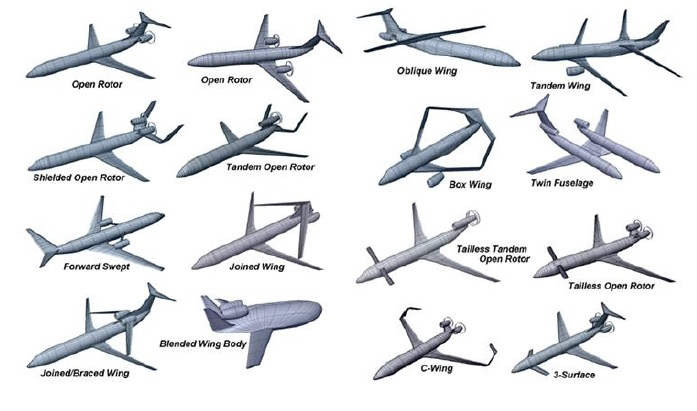
\includegraphics[keepaspectratio, width=0.6\textwidth]{images/chap1/conceptual_design_example.jpg}
	\caption{Example of possible configurations explored in the conceptual design of civil transport aircraft~\cite{bib:raymer_concept_design}.}
	\label{fig:conceptual_design_example}
\end{figure}

As first step, the constraint analysis approach is applied to define the design domain and estimate the necessary thrust~\cite{bib:roskam_partI}; on the basis of this value the engine is chosen, also considering the available technology in the foreseen EIS~\cite{bib:roskam_partII}. 
Then, weight estimation and aerodynamics can be evaluated on the basis of surrogate models, that often use few key parameters, like the wetted surfaces~\cite{bib:roskam_partV, bib:roskam_partVI}.
Performances are often evaluated on the basis of the Breguet equation~\cite{bib:anderson_perfo, bib:roskam_perfo, bib:phillips}.
More accurate methods consist in integrating the set of ordinary differential equations describing the flight dynamics~\cite{bib:roskam_flight_dynamics} using a time step integration~\cite{bib:sforza}, based on the Euler or higher degree methods like the Runge-Kutta scheme~\cite{bib:leveque_partial_equation}.

The aircraft design problem involves multiple disciplines, coupled each others (\textit{e.g.} aerodynamics provides the loads for structural sizing), and thus it may be considered as a Multidisciplinary Design Analysis (MDA).
The MDA is defined as a ``non linear system of equations obtained by the non-intuitive coupling of disciplinary solvers involved in complex engineering systems''~\cite{bib:martins_mdo, bib:gray_omdao}, specifically for this case the conceptual design problem, whereas each discipline provide a set of equations that is coupled with other disciplines.
The generic sizing procedure is given by Schmollgruber in his Ph.D. work~\cite{bib:schmollgruber_phd}; the scheme is presented in Fig.~\ref{fig:aircraft_design_xdsm}, using the \acs{xDSM} standard~\cite{bib:lambe_xdsm}.
Since this standard will be used throughout all this manuscript, it is a important to get familiar with it. 
In this notation the purple circular block represents the optimiser, meanwhile the orange one refers to a \acs{MDA} loop.
Green blocks represent the analysis, numbered according to the order of processing, and pink rectangles represent the functions.
The main workflow is identified by the black line; gray lines represent instead the data sharing.
Analyses outputs are indicated with a grey block, and finally I/O data are identified with a white block: inputs are at the top row, as outputs are at the left column.
For what it concerns the notations, $\underline{x}$ represents the design variables vector, $\underline{y}$ the state variables, apex $(0)$ indicates an initial guess, $t$ a target variable (that is, a variable that is a copy of a previous output) and $(*)$ the final value.  
Algorithm~\ref{alg:aircraft_design} reports the description of analyses, with the numbering that refers to what are used in Fig.~\ref{fig:aircraft_design_xdsm}. 
For a more detailed description refers to the already mentioned work~\cite{bib:schmollgruber_phd}.
\begin{figure}[!h]
	\centering
	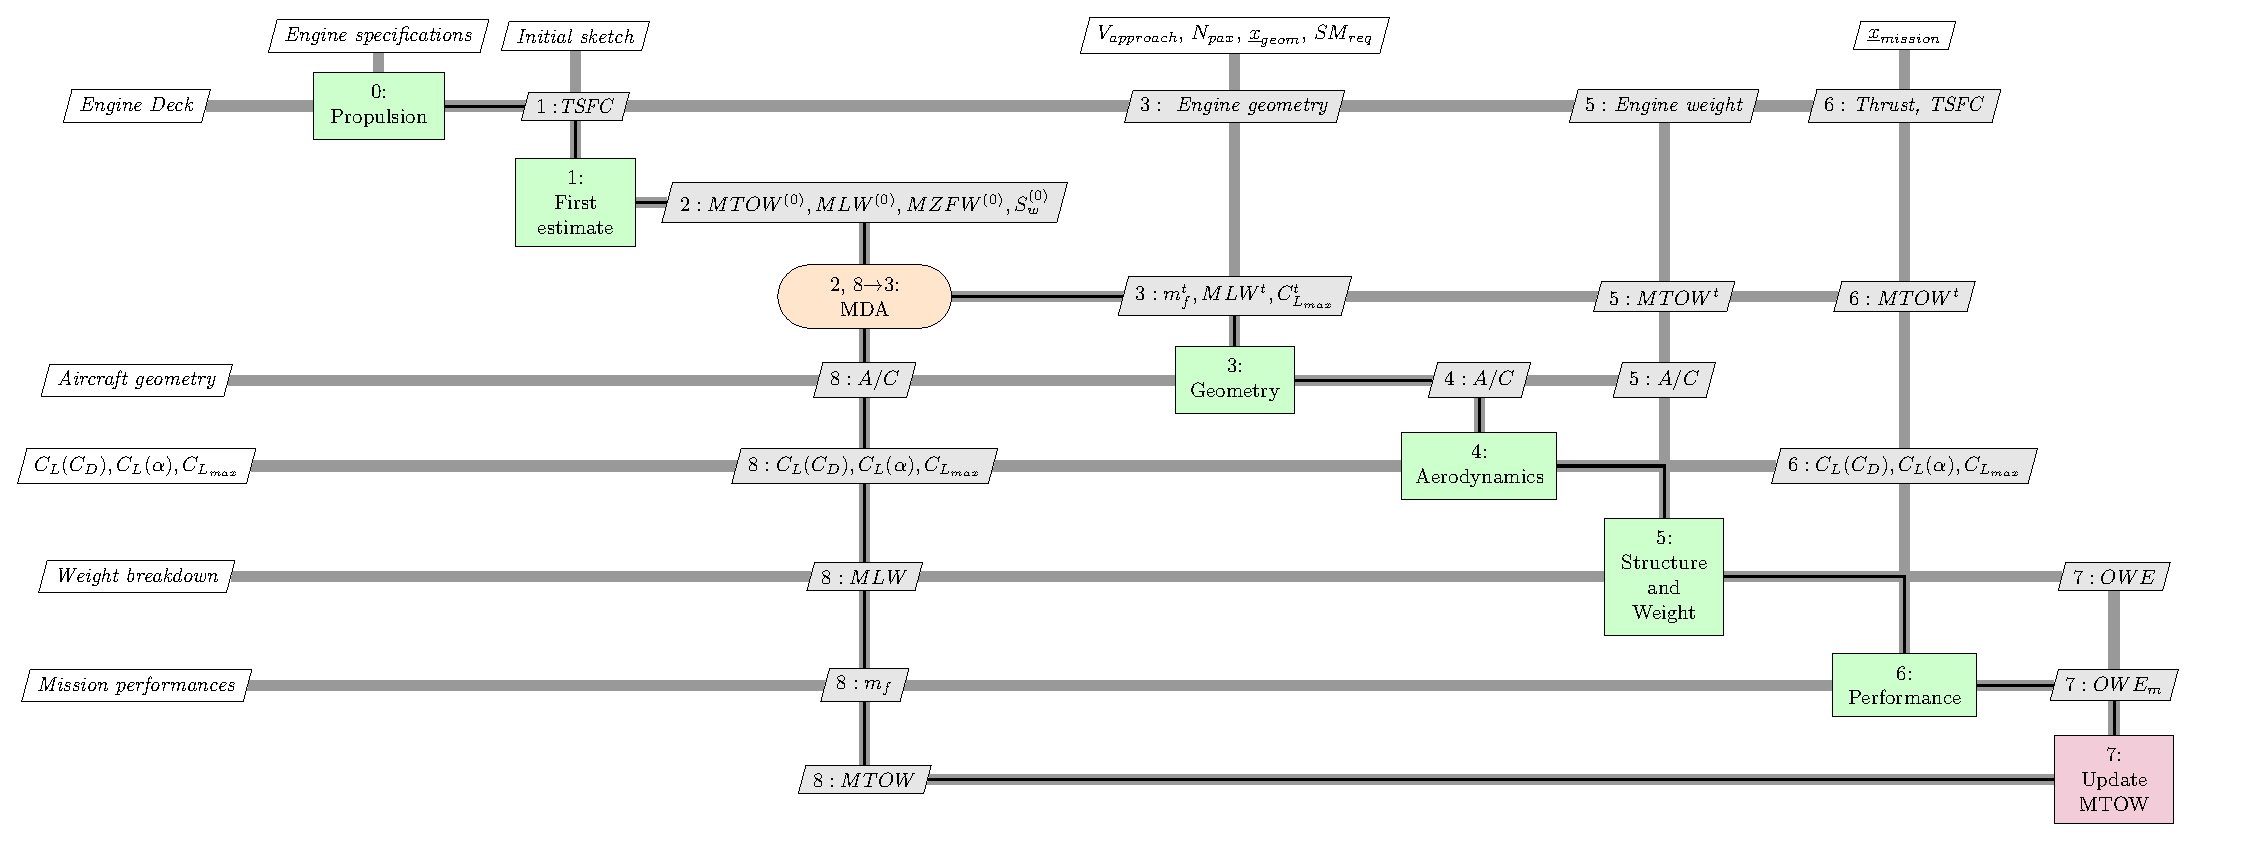
\includegraphics[keepaspectratio, width=1.2\textwidth, angle=90]{images/chap1/MDA_aircraft_design}
	\caption{Preliminary design process, using the xDSM standard presented by Lambe and Martins~\cite{bib:lambe_xdsm}.}
	\label{fig:aircraft_design_xdsm}
\end{figure}

\begin{algorithm}[!h]
	\caption{Preliminary design process algorithm. Numbering is referred to the xDSM presented in Fig.~\ref{fig:aircraft_design_xdsm}.}
	\label{alg:aircraft_design}
	\begin{algorithmic}
		\REQUIRE Initial design parameters (TLAR)
		\ENSURE Sized aircraft, drag polars, masses, design mission trajectory
		\STATE 0: Engine initialization.
		\STATE 1: Compute the initial sizing point (first estimation of wing area $S_w$, Maximum Takeoff Weight MTOW, \dots)
		\STATE 2: Initialise the loop.
		\REPEAT
		\STATE 3: Get the aircraft geometry.
		\STATE 4: Compute the aerodynamics.
		\STATE 5: Perform the structure analysis and get the weight of all the aircraft's components.
		\STATE 6: Compute performance.
		\STATE 7: Update the MTOW value.
		\STATE 8: Check the convergence: if the tolerance is below the desider thresold, return the sized aircraft, otherwise proceed to next iteration.
		\UNTIL {$8 \rightarrow 3$: MDA has converged}
	\end{algorithmic}
\end{algorithm}

In the illustrated case, engine is initialised outside the loop: one of the finding for the designers is to search for an existing engine that matches the fuel consumption targets, or to design a tailored one~\cite{bib:mattingly, bib:roux}. 
The iterative loop calls all the key disciplines involved in aircraft design: geometry, aerodynamics, structures and performance. 
Convergence is driven by the operating weight empty OWE: process is over when the value computed by structural analysis (step 5) is equal to the value computed by performance analysis (state 6).  
It must be noted that disciplines share variables, and thus are coupled each others; \textit{i.e.} structures and weight depend on the aerodynamics results, and the improvement in one of these two disciplines can lead to a degradation in the other one.
At the end more design choices can be made on the final layout, considering also the subsystems~\cite{bib:roskam_partIII, bib:roskam_partIV}. 

It is evident that the aircraft design is a matter of choosing the best compromise between the disciplines that can be considered during this phase or later (\textit{i.e.} acoustic, aeroelasticity, \dots). 
After having sized the aircraft according to given requirements, it is also worthy to study its performance on a set of operational missions, different from the design one: in general, during its life aircraft needs to supply a huge variety of missions, rarely equal to the design one~\cite{bib:roskam_partVIII}.
Tradeoff studies regarding stability or control have low priority in conceptual design phase, but can be included with very easy models, to have a first estimation before the preliminary design phase~\cite{bib:roskam_partVII}.
The Digital Datcom tool~\cite{bib:datcom} is a powerful tool to estimate stability derivatives with the help of the USAF manual~\cite{bib:datcom_ref}: data results come from statistical data on commercial aircraft and allow to size with limited approximation wing and tails~\cite{bib:sforza}. 
Despite the advantages, this tool is limited to conventional configuration, and is not reliable when the aircraft architecture differs from a TAW configuration. 

Clearly, at this point there are some uncertainties, associated to both the methods used and the perspective on the available technologies for the EIS considered; a good practice to approach this issue is through the use of some corrective factors~\cite{bib:kirby}, to assess the sensitivity with respect to technological parameters. 
The choice of the preferred configuration can be guided also by other considerations, like a preliminary cost assessment~\cite{bib:roskam_partVIII}. Once that a configuration is chosen, it is possible to proceed through the preliminary design phase, aimed to study with more detailed models to better undestand if the proposed aircraft can fulfill the customer requirements with a reasonable given cost. 

To conclude this paragraph, the conceptual design phase is well assessed for conventional configuration, but may be unable to deal with innovative concepts; however it represents the state of the art today and the starting point for future development. 

Next section reports a bibliographic review on the most promising technologies for next generation aircraft, which will be helpful in defining a promising concept to cope with environmental goals. 

\section{Key innovative aircraft technologies}
\label{sec:chap1_key_innovative_techno}

One of the \textit{leitmotiv} of aviation has always been the reduction of fuel consumption, related to emission and costs for airlines. 
For this reason, the research of innovative technologies has always been a priority in aircraft design, and with the rise of environmental constraint the works about this subject have been multiplied year by year.

Innovation can be brought at mainly two levels: architecture and propulsion~\cite{bib:isikveren_2014}. 
To the first category belong all the configurations deploying new technologies to increase the aerodynamics efficiency (expressed by the lift-to-drag ratio LoD), \textit{e.g.} the strut braced wing~\cite{bib:gur} or the active flow control~\cite{bib:iata, bib:iata_annex}.
To the second category, instead, belong the aircraft that presents innovation at propulsive level, \textit{e.g.} the Airbus Neo generation which mount high by-pass ratio (BPR) engines~\cite{bib:hughes}, or proposed concept whereas the propulsive plant has been completely modified to go towards electric/hybrid propulsion~\cite{bib:pornet_journal_he, bib:campbell_prop, bib:lambert}. 

The last case is one of the most interesting from an environmental point of view, since the possibility to employ electric source for propulsion may allow the desider emission reduction~\cite{bib:hepperle, bib:vanbogaert}.
Fostered by promising results in automotive industry, some manufacturers have already entered in the commerce with small electric aircraft; in particular it is to note the experience of Pipistrel~\cite{bib:pipistrel_alpha, bib:pipistrel_taurus} and Lange Aviation~\cite{bib:antares_main, bib:antares}. 

In practice, the challenges of designign aircraft with new propulsive systems require a cross-disciplinary effort that focuses on: feasible propulsion system, reduced fuel consumption, aviation safety and reliability, noise reduction, and optimised aircraft design to achieve desiderable performance~\cite{bib:liu_2018}. 
Starting from the very basic performance, even the Breguet equation loses its validity for this category of aircraft, and must be reformulated~\cite{bib:hepperle, bib:marwa}.
The definition of a proper powerplant is not a trivial aspect~\cite{bib:isikveren_celiner}, and also acceptance to passengers is of relevance in the introduction of such disruptive concept~\cite{bib:hornung}. 
Nevertheless, many authors, such as Freeman et al.~\cite{bib:freeman} or Seitz et al.~\cite{bib:seitz_2012}, note that new propulsive system based on hybrid/electric technologies opens new and still unexplored scenarios that may potentially be beneficial from a performance point of view. 
Campbell in its work identifies hybrid/electric propulsion as the most promising solution for revolutionary propulsion~\cite{bib:campbell_prop}.

It is to note that the electric aircraft already flying today are within the segment of small aircraft (two or four seater), whereas the most critical segment on which an action is needed is the single aisle large passenger aircraft, as shown also in the breakdown of Fig.~\ref{fig:aviation_emission_breakdown}. 
Conceptual studies to cover this segment are available in literature; next section will survey some of them to understand their impact and possible benefit. 

\subsection{Hybrid and electric propulsion technology}
\label{subsec:chap1_he_aircraft_key_techno}

This section focuses more on the concept, proposed in literature, to match the environmental goals of Table~\ref{tab:nasa_armd_table}, and thus have a long-term entry into service, except for the NASA X-57.
The study of large passenger aircraft featuring hybrid and electric (HE) propulsion has started in last decade within the NASA funded projects, as the N+3~\cite{bib:follen_nasa_np3} and the SUGAR~\cite{bib:bradley_sugar_p2, bib:bradley_sugar_p2_v2}, the Aurora D8 program~\cite{bib:aurora_d8_ref}, the PEGASUS concept~\cite{bib:pegasus}, the ECO-150 aircraft~\cite{bib:schiltgen, bib:freeman_eco150}, or the CE-Liner proposed by Bauhaus~\cite{bib:hornung, bib:steiner}, just to give some examples. 

The key aspect in these studies is the perspectives of available technologies in long-term: nowadays the exploration of the superconducting devices has started, and they show better performance than the non cryogenic technologies~\cite{bib:dever, bib:madavan}. 
The great advantage of the superconductors theory is that it eliminates the thermal management unit, which represents one of the most relevant weight penalties, and a main aspect in the sizing of electric aircraft, that can not be neglected~\cite{bib:freeman}.

Among the possibilities introduced by the hybrid/electric propulsion, two main features have been identified: distributed propulsion~\cite{bib:gohardani_book} and Boundary Layer Ingestion device~\cite{bib:smith_bli}. 
They have been noted because of their interest in terms of aero-propulsive integration and propulsive efficiency, confirmed by different authors~\cite{bib:borer_sceptor, bib:welstead_2017}, and thus they are reviewed more in detail; before going thorough these topics, some notions on hybrid/electric architecture are introduced in next paragraph. 

\subsubsection{Hybrid propulsion fundamentals}
\label{subsubsec:chap1_elec_fundamentals}

A dual-energy source aircraft can be categorised using the degree of hybridization, initially defined by Isikveren et al.~\cite{bib:isikveren}. 
The degree of hybridization is a figure of merit of the aircraft hybridization, that can be related to the power or the energy. 
It is defined as the power/energy demanded to the secondary source over the total:
\begin{subequations}
	\begin{equation}
		\label{eq:hp}
		H_P = \frac{P_{elec}}{P_{tot}}
	\end{equation}
	\begin{equation}
		\label{eq:he}
		H_E = \frac{E_{elec}}{E_{tot}}
	\end{equation}
\end{subequations}

It is to remark that the $H_P$ and $H_E$ are referred to a dual-energy source aircraft, but they do not depend by the type of sources: electric power can be delivered by batteries such as other devices, without losing any generality.
By definition, a conventional aircraft has $H_P=H_E=0$.
With the help of these definitions, four types of aircraft can be recognised, the scheme of which is shown in Fig.~\ref{fig:he_architectures}: 
\begin{itemize}
	
	\item All electric aircraft, that use exclusively electric energy and power (Fig.~\ref{fig:all_electric}).
	
	\item Turboelectric aircraft, that use combustable for energy storage but electric power to drive the propulsors (Fig.~\ref{fig:turbo_electric}).
	
	\item Series hybrid aircraft, where electrical power is supplied by the two sources that work together and are connected through an electrical node, called bus (Fig~\ref{fig:series_hybrid}).
	
	\item Parallel hybrid aircraft, where the engine provides power to propulsors mechanically. Combustion engine may use electrical power to reduce the fuel flow~\cite{bib:bradley_sugar_p2_v2}, or clutch-off to allow full electric segments~\cite{bib:ausserer} (Fig.~\ref{fig:parallel_hybrid}).
\end{itemize}

\begin{figure}[!h]
	\centering
	\begin{subfigure}{0.3\textwidth}
		\centering
		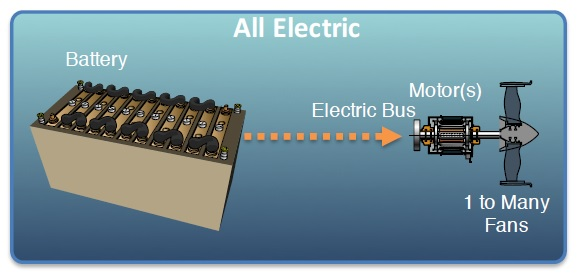
\includegraphics[width=\linewidth, height=0.15\textheight]{images/chap1/all_electric.jpg}
		\caption{All electric.}
		\label{fig:all_electric}
	\end{subfigure}
	\hspace{10mm}
	\begin{subfigure}{0.3\textwidth}
		\centering
		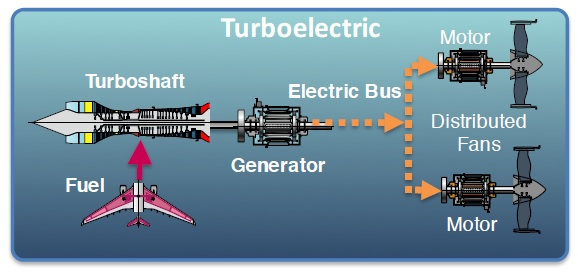
\includegraphics[width=\linewidth, height=0.15\textheight]{images/chap1/turboelectric.jpg}
		\caption{Turboelectric.}
		\label{fig:turbo_electric}
	\end{subfigure}
	\\
	\begin{subfigure}{0.3\textwidth}
		\centering
		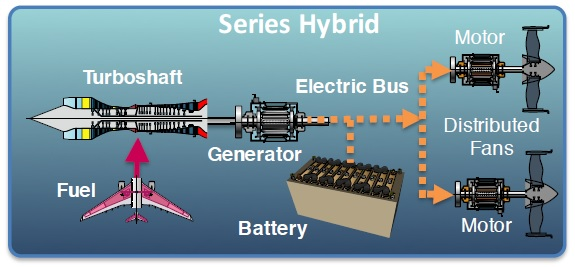
\includegraphics[width=\linewidth, height=0.15\textheight]{images/chap1/series_hybrid.jpg}
		\caption{Series hybrid.}
		\label{fig:series_hybrid}
	\end{subfigure}
	\hspace{10mm}
	\begin{subfigure}{0.3\textwidth}
		\centering
		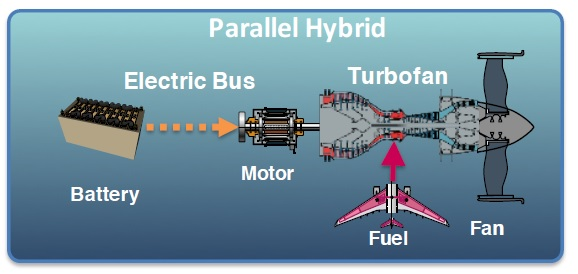
\includegraphics[width=\linewidth, height=0.15\textheight]{images/chap1/parallel_hybrid.jpg}
		\caption{Parallel hybrid.}
		\label{fig:parallel_hybrid}
	\end{subfigure}
	\caption{Different electric propulsion architectures~\cite{bib:madavan}.}
	\label{fig:he_architectures}
\end{figure}

The categories just described are classified according to the degree of hybridization as in Table~\ref{tab:he_architectures}: the classification is clear recalling the definition of $H_P$ and $H_E$.
\begin{table}[!h]
	\centering
	\begin{tabular}{l r r}
		\hline
		& $H_P$ & $H_E$ \\
		\hline
		Conventional & 0 & 0 \\
		All-electric & 1 & 1 \\
		Turboelectric & >0 & 0 \\
		Series hybrid & 1 & <1 \\
		Parallel hybrid & <1 & <1 \\
		\hline
	\end{tabular}
	\caption{Classification of electric propulsion architectures, based on the degree of hybridization.}
	\label{tab:he_architectures}
\end{table}

In an hybrid electric architecture the key points for the sizing are the power and the energy requirements: each component needs to supply a certain amount of power. 
For this reason, when evaluating this kind of concept, the two most important technological parameters, for each device, are the specific power and the specific energy~\cite{bib:fraunhofer, bib:naec}, defined respectively as the energy or the power per unit of mass. 
Specific energy content is particularly valuable for batteries design, since these elements must store a certain amount of energy, meanwhile specific power is the key design parameter for electric components that must deliver certain amount of power. 
Following the examples of Pornet et al.~\cite{bib:pornet, bib:pornet_book} and Brelje and Martins~\cite{bib:brelje_biblio}, the notation here adopted uses the lowercase to represent specific quantities of the extensive quantity: \textit{i.e.}, $e$ indicated the specific energy density and $p$ the specific power density. 

Together with the specific quantities, also the volumetric densities are relevant, since the volume available constrains the integration of the electronic systems. 
Specific and volumetric densities are related through the physical density:
\begin{subequations}
	\begin{equation}
	\rho_E = \rho e 
	\label{eq:energy_density}
	\end{equation}
	\begin{equation}
	\rho_P = \rho p
	\label{eq:power_density}
	\end{equation}
\end{subequations}
where $\rho_E$ and $\rho_P$ are the energy and power volumetric content, and $\rho$ the physical density. 

The main challenge facing HE aircraft is that batteries specific energy content is 50 times lower than that of fuel: \textit{i.e.}, for the fuel $e_f$=11900~\si{\kilo\watt\hour\per\kilogram}, meanwhile for a classical Lithium-Ion battery $e_b$=200~\si{\kilo\watt\per\kilogram}, for today's technology~\cite{bib:rheaume}.
This is also shown in Fig.~\ref{fig:energy_storage_properties}, that presents the energy characteristics for different energy storage systems. 
\begin{figure}[!h]
	\centering
	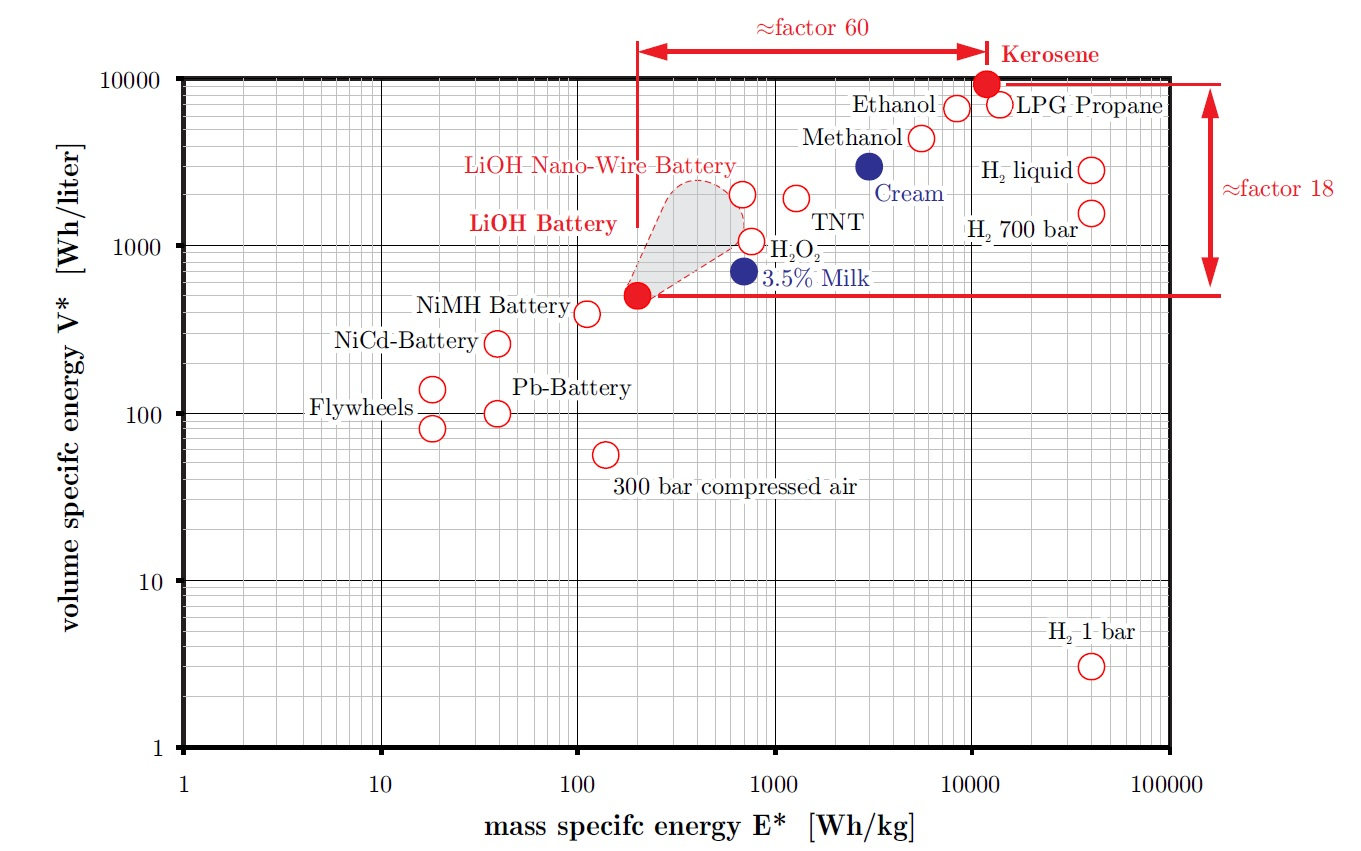
\includegraphics[width=0.8\linewidth, keepaspectratio]{images/chap1/energy_storage_properties.jpg}
	\caption{Mass specific energy vs. volume specific energy for different energy storage systems~\cite{bib:hepperle}.}
	\label{fig:energy_storage_properties}
\end{figure}

From the diagram emerges that hydrogen has a very large specific energy, even larger than the kerosene, but at standard pressure the volume content is poor, and thus it requires large volumes for the allocation. 
The problem can be avoided pressurizing the hydrogen, or using it at liquid state with a cryogenic technology, but difficulties in the identification of a sustainable production, storage and delivery system make this technology unfeasible for aviation, considering today's technological capabilities~\cite{bib:rondinelli}.

The problem of mounting and dismouting batteries' package has been addressed by Pl\"{o}tner et al.~\cite{bib:plotner} in the case of CE-Liner, and in their work they showed that integration of batteries in airframe, as well as airport operations (mounting/dismounting) do not present particular issue, for today's technology. 
Among the different types, LiOH batteries are the most perfoming, with the highest energy and volume content, that allow to have a certain amount of energy still with a feasible volume that can be mounted on aircraft.  
However, the huge difference with respect to kerosene characteristics limits the range of application: batteries introduce in fact a weight penalty, resulting in a bigger MTOW for HE aircraft. 
As a consequence, this concept is not feasible for long range distances, where the effect of carrying heavy batteries outweights the total energy advantage coming from the hybridization: its major interest is within the short and medium range segment.  

Finally, to conclude this overview on the hybrid and electric aircraft fundamentals, a metric to assess the ``goodness'' of the hybrid/electric concept must be defined.
Some of the parameters used for conventional aircraft work fine also for the hybrid electric architecture~\cite{bib:brelje_biblio}, \textit{e.g.} the fuel burn or the MTOW~\cite{bib:roskam_partVIII, bib:thorbeck}. 

Acquisition and direct costs are also relevant as metrics, specially for airlines. 
Pornet et al. preented new models for the cost evaluation, that consider the substitution of an internal combustion engine (ICE) with new hybrid power plant~\cite{bib:pornet_cost}.

Then, literature proposes other metrics: among all the possibilities, for hybrid electric aircraft are particularly relevant the energy specific air range ESAR~\cite{bib:pornet_cost, bib:ploetner} and the payload fuel energy efficiency PFEE~\cite{bib:hileman}, plus some other metrics for propulsion system performance evaluation, that prescind to the propulsive system itself and can be applied for conventional, hybrid and electric aircraft~\cite{bib:schmitz_2013}.
The ESAR quantifies the distance flown per unit of energy, and it is directly derived from the specific air range SAR (distance flown per mass of fuel). Higher the ESAR, better is the aircraft. 

The disadvantage of the ESAR, as similar metrics, is that it does not consider the payload: according to the ESAR, an aircraft that is not carrying any payload results more efficient than a loaded aircraft, when in reality the first one is not useful, since the main scope of the aircraft is to carry a certain payload from one point to another. 
To include also the useful carried weight, Hileman~\cite{bib:hileman} defined the PFEE as the range-payload per unit of energy consumed: 
\begin{equation}
	\label{eq:pfee}
	PFEE = \frac{\textrm{R} m_{PL}}{E_c}
\end{equation} 
This metric identifies an efficient aircraft as that one able to carry for longer distances a certain payload, with less energy, so it includes all the key aspects in the aircraft design. 
Unified propulsion system performance metrics proposed by Schmitz can be applied to all types of propulsion, but they do not consider the integration within the overall design and they are tailored purely to evaluate propulsive performance.
PFEE, instead, represents the most complete figure of merit to assess the validity of the hybrid concept.

\subsubsection{Distributed propulsion technology review}
\label{subsubsec:chap1_dep_review}

The distributed propulsion architecture addresses the problem of how to improve propulsive efficiency $\eta_p$.
This quantity depends on the fan pressure ratio (FPR) as follow ~\cite{bib:felder_2009}:
\begin{equation}
	\label{eq:prop_eff_fpr}
	\eta_p = 0.98 - 0.08\left(\textrm{FPR}-1\right)
\end{equation}

Engine's manufacturers have been working for years to reduce the FPR and increase $\eta_p$, but the procedure presents a relevant drawback: to keep the same thrust level, a reduced FPR requires a bigger mass flow rate passing through the fan.
This reflects on greater fan dimensions~\cite{bib:dragon}.
As example, Fig.~\ref{fig:a320_engine_comparison} shows a comparison between the engine's dimension of the A320 and its evoluted configuration, the A320Neo, mounting the new LEAP engine~\cite{bib:leap_engine}.
\begin{figure}[!h]
	\centering
	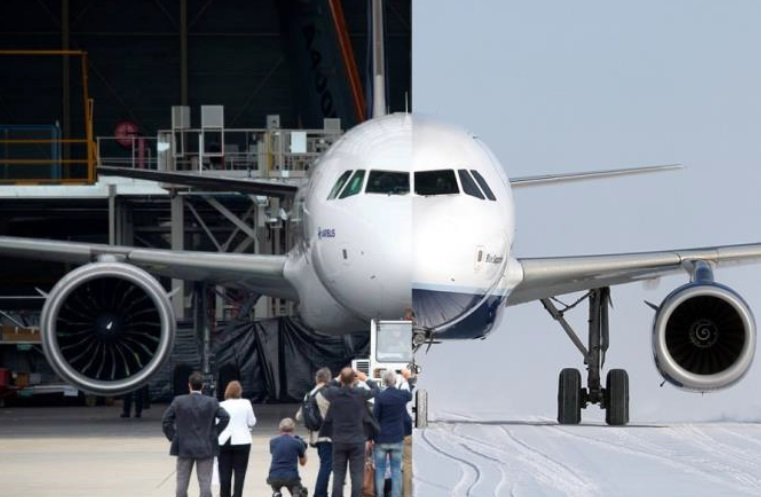
\includegraphics[keepaspectratio, width=0.6\textwidth]{images/chap1/a320_engine_comparison.jpg}
	\caption{Comparison between the Airbus A320 (right) and the new A320 Neo (left) mounting the innovative LEAP engine.}
	\label{fig:a320_engine_comparison}
\end{figure}
It is clear that it is not possible to continuously reduce the FPR, because the advantages of having a better propulsive efficiency will be counterbalanced by the augmentation in drag due to the bigger wetted surfaces. 

In this context, the distributed propulsion (DP) has a major interest, since it allows to distribute thrust on a given set of engines, with a smaller power requirement than the classical two engine configurations~\cite{bib:ko, bib:kirner, bib:dragon}. 
So with the help of DP it is still possible to reduce the FPR, keeping dimensions limited. 

As seen in previous section, the DP represents a key technology that has been massively explored in recent years.
Gohardani is one of the pioneer of the DP, and collected in a single paper all the milestones of such system, from early years to today~\cite{bib:gohardani}, and opened perspectives for its application in the electric aircraft. 
It is to underline that the DP technology is applied without considering the energy source: they can be propellers, ducted fans, moved by turboshafts or electric motors. 
Strictly speaking, this technology is related to how the total thrust can be distributed, no matter how it is produced.
To differentiate the two cases, the acronym DP is used to talk about the concept, as DEP (distributed electric propulsion) is linked with the particular application of DP to electric propulsion. 

One of the main example of DEP application to improve the propulsive efficiency is provided by DRAGON, a concept presented by ONERA~\cite{bib:dragon} and shown in Fig.~\ref{fig:dragon}. 
\begin{figure}[h!]
	\centering
	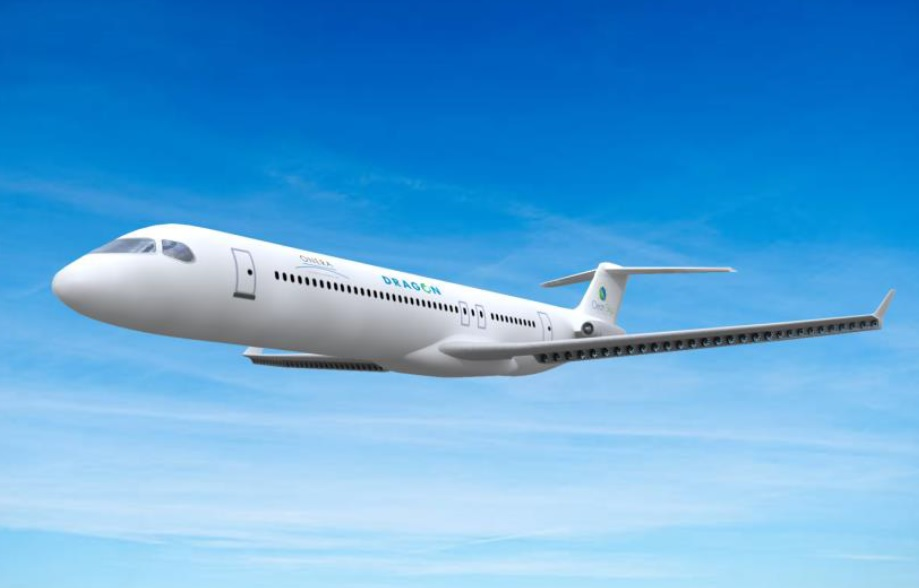
\includegraphics[keepaspectratio, width=0.5\linewidth]{images/chap1/dragon.jpg}
	\caption{DRAGON concept, proposed by ONERA~\cite{bib:dragon}.}
	\label{fig:dragon}
\end{figure}
In this concept two turboshafts provide electric power to the motors, mounted on the wing lower surface.
This concept is represented of the downsizing due to the distributed propulsion, and represents a practical application of DEP applied to the segment of major interest in this research. 
Tradeoff studies on this configuration are promising and identify potential gains with respect to reference conventional aircraft.
Also, this work addresses the problem of the mass variation due to the presence of a distributed propulsion system: in theory, the distributed weight along the wing relax the bending moment at the wing root, resulting in a possible less stiffened structure. 
In practice, the authors explain that this analysis does not include the torsion moment generated by the engines, and some preliminary analyses show that the final weight finally results increases~\cite{bib:dragon}. 
Kim et al. further developed the propulsive and weight aspects, adding some knowledge to the aforementioned work of Gohardany~\cite{bib:kim_dep, bib:kim_dep_review}: they proposed a benchmark of typical weights and aircraft parameters featuring DEP. 

Moreover, the potentiality introduced by DEP are not only limited to a better propulsive efficiency: indeed, the idea is 60 years old and dates back to 1924, when Manzel considered the possibility of distributing propellers over a row~\cite{bib:manzel}.
He had an intuition that in this system aerodynamics and propulsive aspects are correlated; in some experimental work he detected that the region interested by the presence of distributed fan is subject to a blowing, which energizes the fuel. 
In this condition it is possible to potentially have laminar flow with increased lift, resulting in a reduced takeoff and landing length; unfortunately the project has been abandoned for lack of knowledge. 
His idea was further developed at the beginning of the VTOL concepts~\cite{bib:malvestuto}, and it has been further developed up to today; even the basic idea was the same of Manzel, his concept has been brought on a new level, thanks to the knowledge gained in over 80 years~\cite{bib:gohardani_book}. 

The state of the art for the DP application is the NASA SCEPTOR X-57 demonstrator~\cite{bib:borer_sceptor} shown in Fig.~\ref{fig:nasa_x57}. 
\begin{figure}[h!]
	\centering
	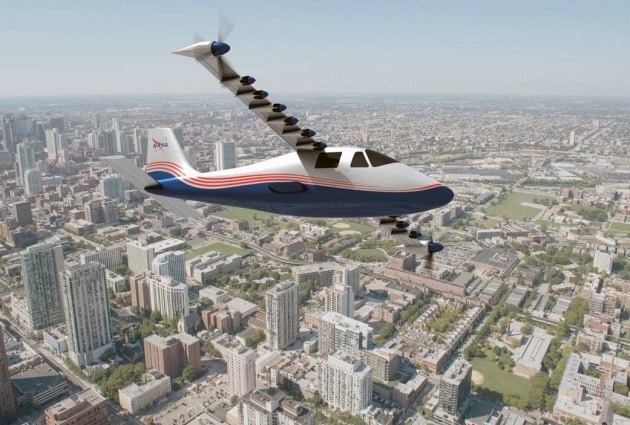
\includegraphics[keepaspectratio, width=0.5\linewidth]{images/chap1/nasa_x57.jpg}
	\caption{NASA SCEPTOR X-57 concept~\cite{bib:borer_sceptor}.}
	\label{fig:nasa_x57}
\end{figure}
It is a small aircraft, based on the existing Tecnam P2006T aircraft, that proposes to use two wingtip propellers, to reduce induced drag, and a certain number of smaller distributed propellers, to take advantages of distributed propulsion through the blowing effect to increase the maximum $C_L$~\cite{bib:deere_2017b}. 
High-lift devices are not needed anymore, leading to an easier and lighter wing structure; however, the distributed propellers require an accurate wing design~\cite{bib:deere_2017a}. 
To avoid problem in cruise, where the blowing worsenes the handling qualities, the small propellers are used only for takeoff and landing, then they are flapped and only the two wingtip propellers are used. 
The electric version of the NASA X-57, sometimes referred as NASA X-57 Maxwell, mounts Lithium-Ion batteries to supply electric power. 
Thermal~\cite{bib:schnulo} and control aspects~\cite{bib:clarke} of this configuration have been studied, then the batteries and the propellers have been optimised with respect to the mission requirements~\cite{bib:hwang_x57}: it is possible to say that the work on the NASA X-57 is the most comprehensive and represents the best example of electric integration benefits. 
It is also a milestone in the distributed propulsion effects on performance and sizing~\cite{bib:moore_2018}. 

Another interesting concept, in the same segment as the X-57, is AMPERE~\cite{bib:ampere_ref}, developed at ONERA and depicted in Fig.~\ref{fig:ampere}. 
\begin{figure}[h!]
	\centering
	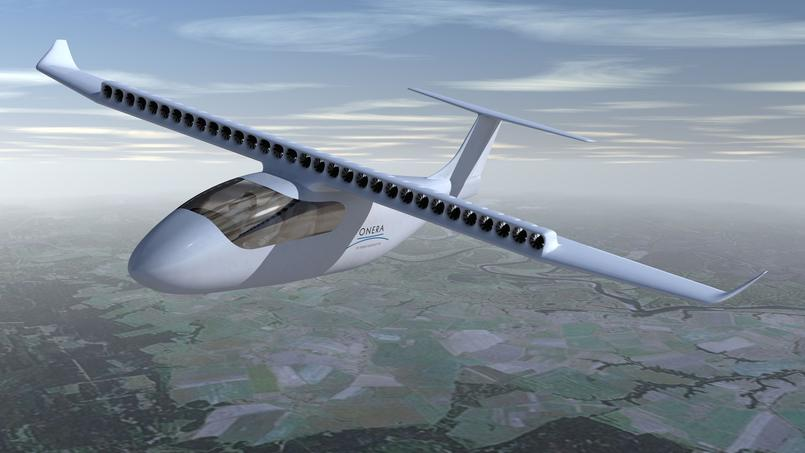
\includegraphics[keepaspectratio, width=0.5\linewidth]{images/chap1/ampere.jpg}
	\caption{AMPERE concept, proposed by ONERA~\cite{bib:ampere_ref}.}
	\label{fig:ampere}
\end{figure}
Instead of having distributed propellers, the propulsion is obtained with a set of ducted fans, distributed along the wing. 
Differently from the previous example, the blowing effect is acting in all the mission phases, and thus to understand how it impacts on the handling qualities wing tunnel tests and simulations have been carried out~\cite{bib:dillinger_ampere}. 

Nevertheless, blowing phenomenon is just one of the aerodynamics effects introduced by DP: Manzel already mentioned the possibility of a laminar flow over the wing, and in recent years Borer et al.~\cite{bib:borer}, for the case of NASA X-57, showed that indeed laminarity is obtained and assessed the related aerodynamics improvement. 
Hovewer, the benefits strongly depend on the engines' position: Wick et al.~\cite{bib:wick} considered three different configurations, with engines over the wing, integrated within the structure and under the wing, and it has been seen that the aerodynamics strongly depends on how the engines are distributed. 
The embedded configurations are even harder to analyse, due to the strong coupling between the aerodynamics and the propulsion, as well as the structural side of building wing with propulsors integrated in the airframe~\cite{bib:khero}. 
Hoogref et al.~\cite{bib:hoogreef}, on the contrary, concluded showing that the DP must be rediscussed, because the advantages can not be so marked as the literature may suggest.
At this stage, further analyses have to be conducted to select the most promising disposition to benefit of DP. 

Another non trivial feature of DP is linked to the possibility of engines downsizing. 
Generally, one of the main requirements to meet in aircraft design is the case of one engine inoperative (OEI)~\cite{bib:roskam_partI}.
This condition in a DP system becomes less stringent: in fact, in case one engine is out, to get the same thrust level the other engines must provide less thrust \textit{i.e.} in case of 4 engines deployed than 2~\cite{bib:steiner}. 
This concept is better illustrated in Fig.~\ref{fig:oei_condition}.   
\begin{figure}[h!]
	\centering
	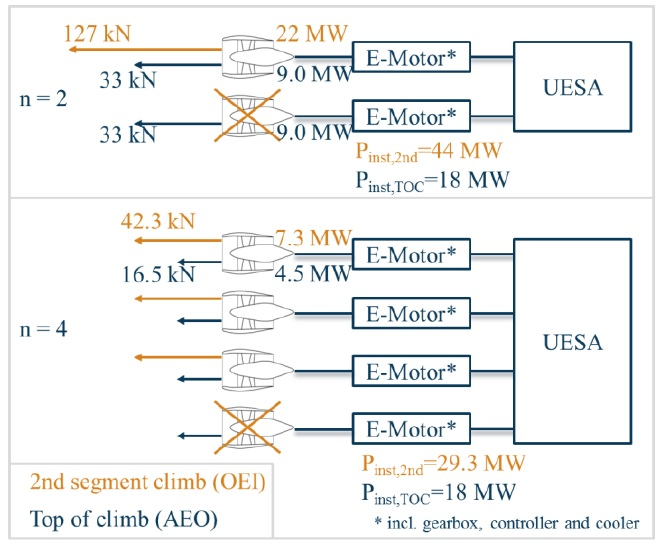
\includegraphics[keepaspectratio, width=0.5\linewidth]{images/chap1/oei_condition.jpg}
	\caption{Illustration showing the difference in the engine sizing to meet the OEI condition for 2 and 4 motors~\cite{bib:steiner}.}
	\label{fig:oei_condition}
\end{figure}
Of course, a lower installed thrust is directly linked to a smaller engines; it is to mention that on a safety point of view the DP may be considered safer than the classical one, since it intrinsecaly adds redundancy. 

Safety aspects of the DP are treated by Papathakis et al.~\cite{bib:papathakis}, but so far a full comprehension of all the issues related to security is still a remarkable challenge.
At this stage, research is still far to define a preferrable arrangement for the engines, to maximise aerodynamics' benefit; also, due to the strong integration between different disciplines, so far the works are limited by the use of high fidelity tools, and thus the DP effects in the overall design process have not been considered yet. 
A clear and shared DP terminology is desiderable in the future to permit to better discuss this emerging technology.
Then, more detailed studies are needed to identify an optimised framework, involving weight, number of propulsion units, and other top level aircraft parameters, to meet a commercial configuration capable to go through a sustainable civil aviation. 

Distributed electric propulsion is only one of the two features identified for hybrid/electric technology, the other one is the BLI, which enhances the advantages of DEP and viceversa, as it will be better detailed in the following section. 

\subsubsection{Boundary layer ingestion device}
\label{subsubsec:chap1_bli_review}

The second aspect identified for hybrid and electric configurations is the Boundary Layer Ingestion (BLI) device: it is one of the core technologies that may impact the distributed propulsion technology.
The BLI idea arose at the beginning for marine applications~\cite{bib:park, bib:roberts} and has been lately applied to aircraft~\cite{bib:tournier, bib:owen, bib:allan, bib:peijian}, mainly in subsonic configurations, but some examples on supersonic jet can be found too~\cite{bib:kumar}.

A non negligeable part of the total drag around a body in a flow comes from the boundary layer~\cite{bib:monti_pt2}; the BLI is a device that reduces this contribution by partially ingestion the boundary layer~\cite{bib:smith}. 
As for the DEP, this technology is not recent: one of the early application comes from the work of Smith and Roberts~\cite{bib:smith_bli} in 1947.
In their work, they compared a conventional turbojet configuration with one having installed boundary layer suction devices within some slots in the wing. 
They assessed a 30\% improvement in fuel efficiency and a 7\% higher optimum cruise speed due to the suction of the boundary layer; also they demonstrated that BLI increases the lift-to-drag ratio, reduces takeoff length and contributes to enhance control characteristics. 
Again, its development has been stopped because of lack of knowledge needed, but the improvement since then allows to consider such device for today's applications.

The main challenge in dealing with the BLI lies in a proper formulation to assess the benefits: since it includes the boundary layer aspects, a fully RANS model needs to be used. 
The most important phenomenon related to BLI is that the flow field results changed: streamlines are not parallel to the body anymore and distorsion occures at the inlet entrance. 
Considering only this effect may result limiting in the evaluation of the BLI benefits; Plas et al.~\cite{bib:plas} report all the physical phenomena that occur in BLI and need to be considered: 
\begin{itemize}
	\item State of the boundary layer coming into the intake;
	\item Inlet design, both outside and inside;
	\item Evolution of the non-uniform inlet flow from intake entrance to engine face;
	\item Distorsion transfer across the fan;
	\item Response of the fan to the distortion, which may impact operability and aeromechanics;
	\item Evolution of the flow downstream of the fan;
	\item Duct losses, which shows an high sensitivity because of low FPR; 
	\item Potential flow separation and unsteadiness of the flow field. 
\end{itemize}

So far, the most common way to treat the BLI is with the help of a RANS model: Gray et al. presented an approach in which these equations are coupled with the propulsion, and the geometry is optimised to maximize the benefits of the BLI in the STARC-ABL concept~\cite{bib:gray}.
The same authors optimised the overall turboelectric propulsion system featuring the BLI~\cite{bib:gray_bli_2018}. 
NASA presented an easier modellisation, yet using high fidelity, based on the entropy calculation and successfully used in the N+3 concept studies~\cite{bib:bwb_n3_vol1, bib:bwb_n3_vol2}; ONERA reported a similar approach, but based on the exergy more than the entropy~\cite{bib:arntz}. 
De la Rosa Blanco et al. considered the BLI as basis for a silent aircraft engine, noting the advantages in noise reduction; they also assessed a gain of about 4\% with respect to the best in class with the BLI~\cite{bib:silent_engine_aircraft}. 
There is no evidence of surrogate models, or semi-empirical equations, capable to deal with this phenomenon at low fidelity, and this may be understandable because of the large number of phenomena to be considered. 

Another issue is the definition of a figure of merit to evaluate performance; different authors use the power saving coefficient PSC, defined as below~\cite{bib:smith}:
\begin{equation}
	\label{eq:psc_bli}
	\textrm{PSC} = \frac{P_{ref}-P_{BLI}}{P_{ref}}
\end{equation}

In the equation above, $P_{ref}$ is the reference power of a non-BLI propulsor and $P_{BLI}$ the power required by the propulsors in case the BLI is mounted: as such, PSC quantifies the reduction in the power needed, on a common configuration, with and without the boundary layer suction. 
It is clear that the BLI represents a key feature and may be beneficial for the emission' reduction, despite the huge number of challenges that it poses. 

The most interesting application of BLI is the STARC-ABL~\cite{bib:welstead_2016}, shown in Fig.~\ref{fig:starc_abl}. 
This concept was born because the NASA wanted to develop a concept feasible in the nearer term, overcoming the high technological barrier set by N+3 program~\cite{bib:bradley_sugar_p2_v2}. 
\begin{figure}[!h]
	\centering
	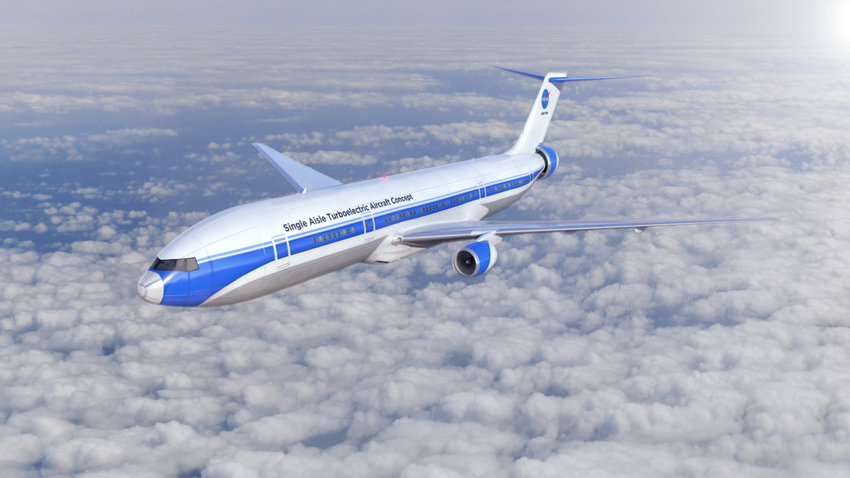
\includegraphics[keepaspectratio, width=0.6\textwidth]{images/chap1/starc_abl.jpg}
	\caption{STARC-ABL concept, proposed by NASA~\cite{bib:welstead_2016}.}
	\label{fig:starc_abl}
\end{figure}
In the STARC-ABL a tailcone propulsor is mounted on a conventional \acs{TAW} fuselage, and it works coupled with two downsized turboshafts, which provide power needed~\cite{bib:yoon}.
The tail-cone propulsor is integrated within the fuselage and mounts a BLI device, capable to ingest around 60\% of the fuselage boundary layer~\cite{bib:welstead_2017}. 
The performance assessment shows a 10-12\% fuel burn reduction thanks to the BLI. 
Another interesting study concerns the dynamic behaviour of the propulsive system, analysed in one of the latest work on STARC-ABL~\cite{bib:kratz}: the dynamic of electric system is indeed an aspect that cannot be neglected during the design of powerplant components; but the level of detail is already higher than that required at conceptual design. 
The program is still active and more studies are foreseen in the next years.

On European side, the CENTRELINE consortium is investigating a concept similar to the STARC-ABL, with propulsive fuselage, called CENTRELINE~\cite{bib:seitz_2018, bib:habermann_2018, bib:bijewitz, bib:goraj}.
The aircraft is depicted in Fig.~\ref{fig:centreline}; an entry into service 2035 is foreseen for the concept.  
\begin{figure}[!h]
	\centering
	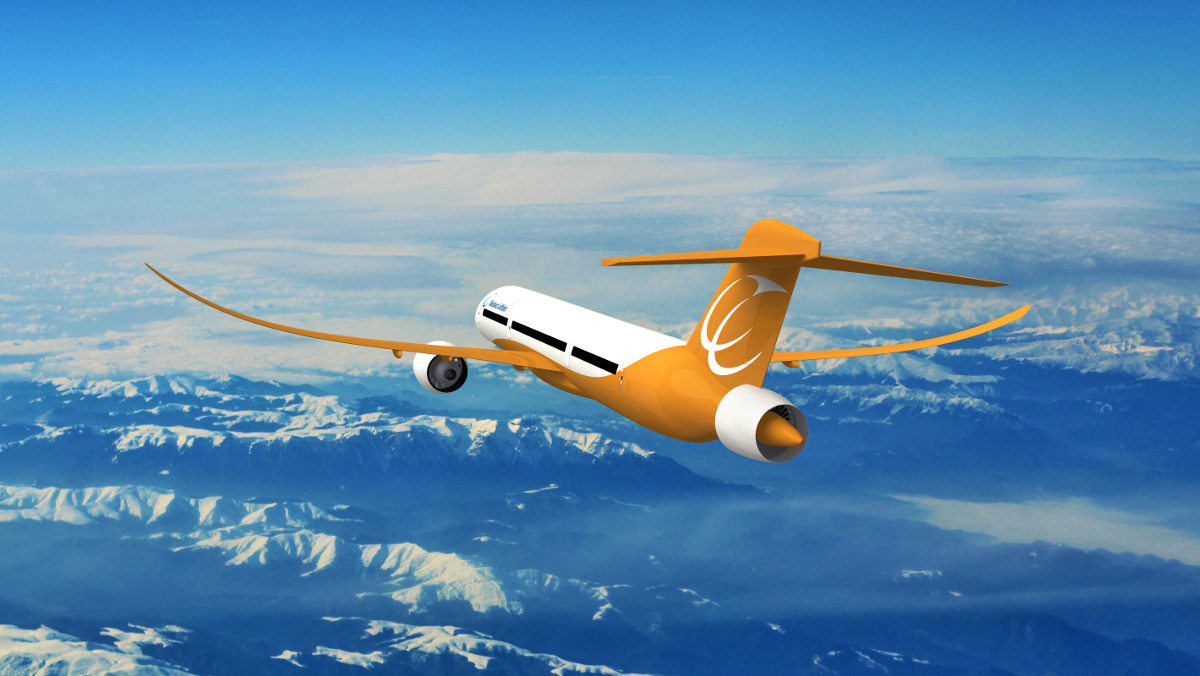
\includegraphics[keepaspectratio, width=0.6\textwidth]{images/chap1/centreline_concept.jpg}
	\caption{CENTRELINE concept, proposed by the CENTRELINE European consortium~\cite{bib:seitz_2018}.}
	\label{fig:centreline}
\end{figure}
Works on the CENTRELINE confirm the potential benefits coming from a propulsive fuselage with a BLI devices, already seen in the STARC-ABL. 
A major point of interest is the design of the powerplant, based on turboelectric configuration, and the technologies adopted~\cite{bib:bijewitz}. 

So far, two different potential technologies to be used in the hybrid and electric frame have been addressed: the DEP and the BLI, which seem to be the most promising features of such a kind of aircraft. 
Actually, these two aspects are not separated, but the DEP is synergistic with BLI, since each one enhances the effect of the other~\cite{bib:gohardani_book}. 
The main question is: which is the best geometry to be considered, to maximize the benefits coming from the DEP coupled with BLI? 
From the experience of the STARC-ABL, the BLI operates better when the reference length is higher: in configurations like the DRAGON one, its effects can be neglected because of the reduced chord length in the wing. 
This has been confirmed by another study on the Nautilius concept~\cite{bib:wiart}, and others~\cite{bib:arntz, bib:plas}. 

Possible candidate to answer the question is the Blended Wing-Body~\cite{bib:liebeck_1998}, in which the whole body is a lifting surface, and the reference length is large enough to take the maximum benefits from a possible integration with DEP and BLI~\cite{bib:bishara}. 
Besided this aspect, the BWB concept offers more space to locate distributed propulsion, maximizing the area subject to the combined effect of blowing and BLI. 
Last but not least, the BWB is a concept designed to maximise the aerodynamic, and thus it shows higher lift-to-drag ratio (values of 22-23 or above are foreseen): it has the potentiality to combine a morphological efficient architecture with enhancement benefits coming from the distributed propulsion. 

Hence, seen the very promising perspectives offered by the BWB, next section investigates more profoundly this configuration, to understand the basic aspects and problems, in order to prepare the field for the discussion regarding a possible integration with hybrid propulsion. 

\subsection{Blended Wing-Body aircraft}
\label{subsec:chap1_bwb}

On a classical TAW configuration, the fuselage is only aimed to carry passengers and luggages, but it is solely a source of drag, being a non lifting component. 
To generate lift in a more efficiency way, it would be better to have all the components generating lift: this is the idea behind the Blended Wing-Body (BWB) concept, where even the passengers' cabin is aerodynamically shaped to contribute to the total aircraft lift. 
McDonnell \& Douglas company was the first to think at the utilisation of BWB for civil transport~\cite{bib:liebeck_1998}, followed by Boeing who proposed a configuration for 450 passengers~\cite{bib:liebeck_2004}: these two examples represent a milestone in the development of this configuration, and they are both shown in Fig.~\ref{fig:bwb_concept_example}. 
\begin{figure}[h!]
	\centering
	\begin{subfigure}{0.4\textwidth}
		\centering
		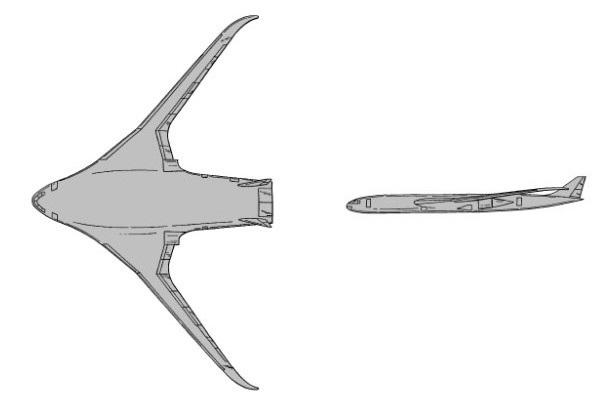
\includegraphics[keepaspectratio, width=\linewidth]{images/chap1/mcdonnell_bwb.jpg}
		\caption{BWB configuration, first proposed by McDonnell \& Douglas in 1998~\cite{bib:liebeck_1998}}
		\label{fig:mcdonnell_bwb}
	\end{subfigure}
	\hspace{10mm}
	\begin{subfigure}{0.4\textwidth}
		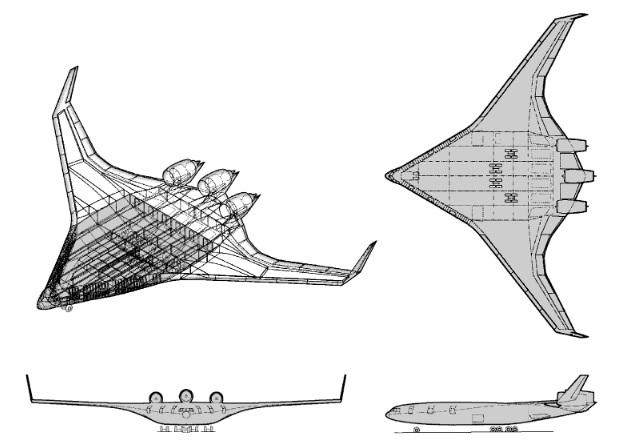
\includegraphics[keepaspectratio, width=\linewidth]{images/chap1/boeing_bwb.jpg}
		\caption{More advanced BWB concept, proposed by Boeing in 2004. This configuration is aimed to carry 450 passengers~\cite{bib:liebeck_2004}.}
		\label{fig:boeing_bwb_450}
	\end{subfigure}
	\caption{Main milestones in the Blended Wing-Body concept.}
	\label{fig:bwb_concept_example}
\end{figure}

The gain in the global lift-to-drag ratio comes mainly from the wetted area reduction: the integration of payload, lift, control surfaces and propulsion in an airfoil shaped centerbody helps to reduce the wetted area of about 30\%~\cite{bib:liebeck_1998}, resulting in a lower friction coefficient and a better efficiency. 
The maximum lift-to-drag ratio is estimated to be likely around 27~\cite{bib:torenbeek_bwb}.
Apart from the aerodynamics aspects, BWB shows also an improved structural efficiency, coming from the lower wing loading and large inertia relief~\cite{bib:liebeck_2004}.
Some studies also confirm that it has reduced the noise, relevant aspect close to ground, \textit{i.e.} during takeoff and landing~\cite{bib:bwb_n3_vol1}. 
Also, the BWB has more available volume to be used for the freight and the subsystem allocations, allowing more flexibility in the center of gravity positioning. 

Despite these advantages, several challenges arise in its design:
\begin{itemize}
	\item Since the cabin it is not cylindrical anymore, the pressurization generates a non-linear stress constraint which varies quadratically with the cabin's width (see Fig.~\ref{fig:pressure_constraint}), resulting in a more complex structural design~\cite{bib:liebeck_1998, bib:mukhopadhayay_2004, bib:mukhopadhayay_2005}. 
	Of course this leads to an increase in mass, compared to a conventional fuselage: the challenge is to design a shell to efficiently carry the pressurization loads, saving weight.
	\begin{figure}[h!]
		\centering
		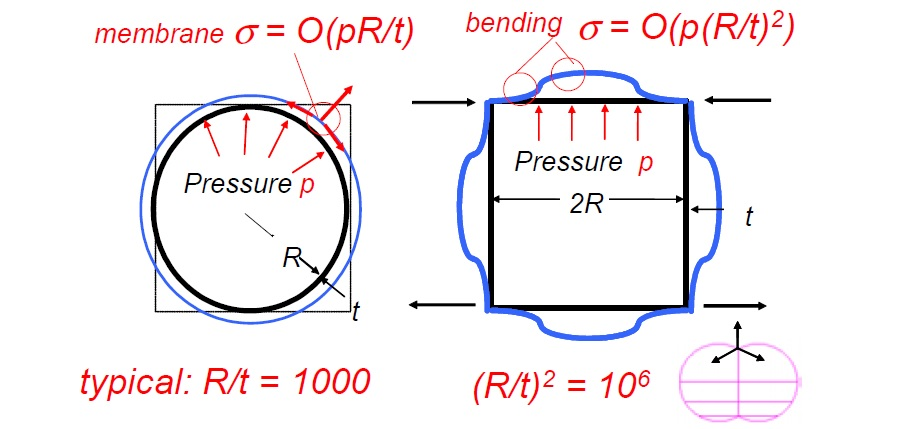
\includegraphics[keepaspectratio, width=0.6\textwidth]{images/chap1/pressurization_constraint.jpg}
		\caption{Different load distributions due to pressurization in a circular (left) and non-circular (right) cabin.}
		\label{fig:pressure_constraint}
	\end{figure}

	\item The BWB is a tailless configuration, so the airfoil design is a key point to obtain a longitudinally stable aircraft~\cite{bib:nickel}, otherwise fly-by-wire systems for the active control have to be inserted, with penalties in weight.
	
	\item Generally, the centerbody trailing edge is used to trim the aircraft at low speed: there is less place for high lift devices and thus $C_{L,\max}$ is reduced with respect to a conventional aircraft.
	
	\item Because of the airfoil-shaped centerbody, the landing gears positioning may represent an issue. 
	In order to have enough space available for this component, the relative thickness must be oversized, and this aspect is more critical especially for small BWB (short and medium range). 
\end{itemize}

These drawbacks make the interest in this concept being lost, because of the high commercial risk; however, it has emerged again in past years.
Nickol et al.~\cite{bib:nickol} considered the BWB as the most promising concept for the aviation environmental sustainability; in the N+3 project the BWB has been deeply studied to assess its performance: the final report from NASA represents a milestone because it provides a comprehensive study of different aspects~\cite{bib:bwb_n3_vol1}, together with an appendix with all the models~\cite{bib:bwb_n3_vol2}. 
Centracchio et al.~\cite{bib:centracchio} got almost the same results as Nickol, comparing a BWB concept with long range best-in-class aircraft.
TU Delft presented two works, one related to the cabin design~\cite{bib:vos_bwb}, and the second one about the parametrization and low fidelity models for evaluate the weights~\cite{bib:brown}; ONERA~\cite{bib:defoort} proposed an OAD procedure for its sizing within the CICAV project; AGILE project studies the definition of an OAD procedure for the BWB sizing, in their paradigma~\cite{bib:prakasha, bib:anisimov}, ISAE-Supaero, together with Airbus, mainly addressed with two Ph.D. projects the problem of the handling qualities~\cite{bib:saucez, bib:denieul}.
Also, it is to mention the study of Bonet, who analysed a scaled BWB geometry in wind tunnel~\cite{bib:bonet}, to confirm numerical results, and the X-48 demonstrator~\cite{bib:boeing_x48}, built from Boeing and NASA on the basis of Liebeck's work~\cite{bib:liebeck_2004} to study control within a flight test campaign, and the experimental work of Cranfield University for the VULCAN concept~\cite{bib:perry}.
Finally, DZYNE (a company based in California, USA) presented a new concept~\cite{bib:dzyne_bwb}, based on an innovative landing gear sizing, which opens this concept for small size, without the drawback of the oversized thickness-to-chord ratio.
They announced the construction of a BWB for an entry into service in the next decade, covering different segments, from the business to long range.
They called it ASCENT, and a visualisation of this concept is provided in Fig.~\ref{fig:dzyne_bwb}, taken from the work of Page et al.~\cite{bib:dzyne_bwb}.
\begin{figure}[h!]
	\centering
	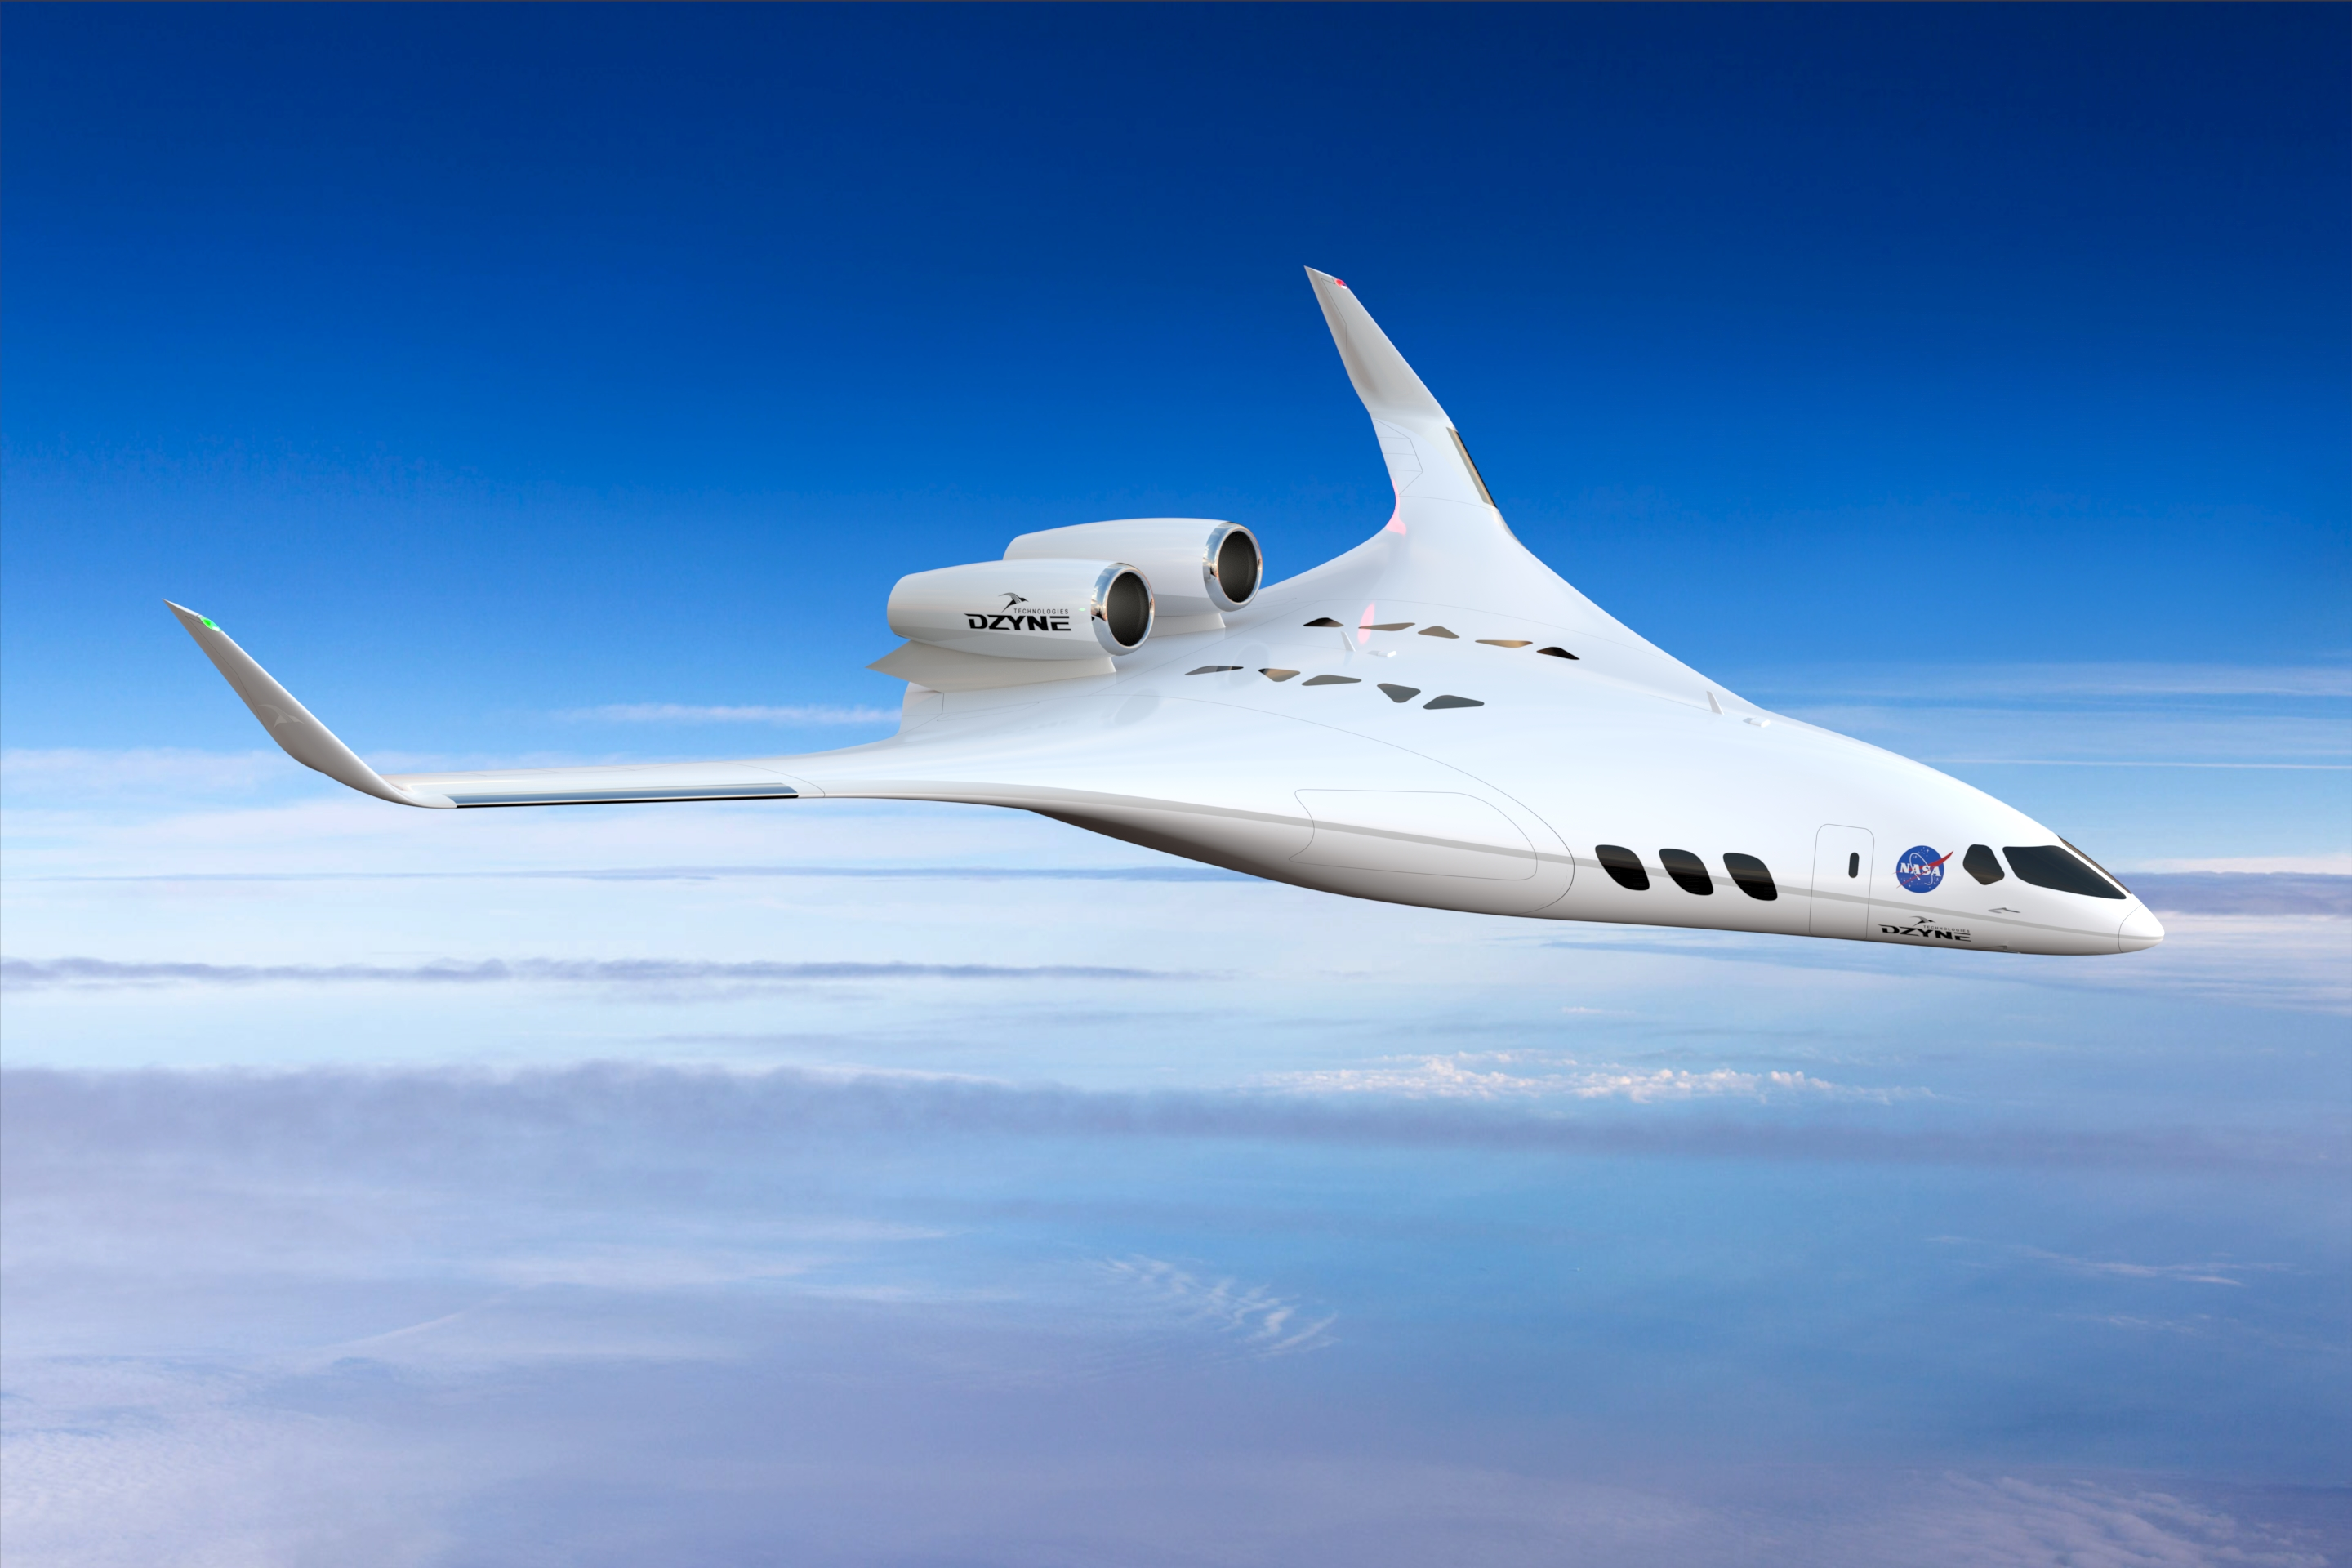
\includegraphics[keepaspectratio, width=0.5\linewidth]{images/chap1/dzyne_bwb.jpg}
	\caption{Rendering of the BWB Ascent 1000, announced by DZYNE and expected to fly in next years~\cite{bib:dzyne_bwb}.}
	\label{fig:dzyne_bwb}
\end{figure}

The examples above indicate how large is the interest in this concept; they are not exaustive of the whole literature on the topic.
Most of cited works cover only structural and aerodynamics aspects, using high fidelity; a minor part is instead deputed to handling qualities and control laws. 
At this stage there are only two evidences in literature of a revised sizing process for the BWB: NASA has implemented surrogate model for the cabin design, with aerodynamics correction, in its in-house code called FLOPS~\cite{bib:bradley_bwb}, but its development has been stopped~\cite{bib:brelje_biblio}.
Van Dommelen and Vos~\cite{bib:van_dommelen} presented a conceptual tool for the BWB design, based on classical methods that can be found in Roskam's books~\cite{bib:roskam_partI}. 

Another difficulty is that there is no availability of public reference data, to build surrogate models to use in preliminary design, with some exceptions as the FLOPS code, the aforementioned work of Van Dommelen and Vos~\cite{bib:van_dommelen}, and the database of NACA for the Northrop YB-49 aircraft, which is a delta wing aircraft, precursor of modern BWB~\cite{bib:robinson, bib:ashkenas}.
In the following two paragraphs, the problem of structural and aerodynamics design for a BWB is addressed, to prepare the field for a possible modelling approach, to be integrated in the conceptual design cycle.

\subsubsection{Structural design of Blended Wing-Body concept}
\label{subsubsec:chap1_bwb_structure}

The cabin structure is the most challenging aspect in designing the BWB: it must carry passengers (and eventually payload) and sustain both pressurization and aerodynamics loads. 
In literature it is possible to find three main propositions: integrated, segregated and oval structure. 
The first two were proposed by Liebeck~\cite{bib:liebeck_1998}, the third one has been explored by Vos et al.~\cite{bib:vos_bwb}. 
Vos et al. also suggest the following element to be considered when analyzing the cabin design:
\begin{itemize}
	\item Design simplicity; 
	\item Passenger evacuation;
	\item Passenger comfort;
	\item Structural efficiency; 
	\item Aerodynamics efficiency.
\end{itemize} 

The three cabin concepts have been considered by different authors dealing with structural design~\cite{bib:mukhopadhayay_2004, bib:mukhopadhayay_2005, bib:qian, bib:hansen}; more details about are reported in Appendix~\ref{app:bwb_cabin_design}. 
What is of interest in this context is the decision analysis reported in Table~\ref{tab:bwb_cabin_structure_synthesis} and based on the cited work.
In Table~\ref{tab:bwb_cabin_structure_synthesis}, a value of +1 is assigned whereas there is an advantage using a certain concept, 0 if an aspect may be an issue, but no relevant and -1 whereas a concept introduces a penalty. 
\begin{table}[!h]
	\centering
	\begin{tabular}{l| c| c| c|}
		\cline{2-4}
		& Integrated & Segregated & Oval \\
		\hline
		\multicolumn{1}{|l|}{Design complexity} & +1 & -1 & -1 \\
		\multicolumn{1}{|l|}{Passenger evacuation} & +1 & -1 & +1 \\
		\multicolumn{1}{|l|}{Passenger comfort} & 0 & +1 & +1 \\
		\multicolumn{1}{|l|}{Structural efficiency} & 0 & +1 & +1 \\
		\multicolumn{1}{|l|}{aerodynamics efficiency} & +1 & +1 & 0 \\ 
		\hline
	\end{tabular}
	\caption{Decision matrix for the three BWB cabin concepts proposed in literature. Values are assigned as follow: +1 if there is a good improvement, 0 if it may be an issue, but not relevant and -1 if it introduces a penalty.}
	\label{tab:bwb_cabin_structure_synthesis}
\end{table}

Table~\ref{tab:bwb_cabin_structure_synthesis} shows that the most interesting concept is the integrated one, since it conjugates a non complex design with acceptable passenger comfort and evacuation and good structural and aerodynamics efficiency: indeed, it has been largely used in different studies on the BWB structural design~\cite{bib:pitera, bib:kawai, bib:hileman_bwb, bib:bradley_bwb, bib:cheng}. 
These works use finite element method, with a detailed structure, to get an estimation of the structural mass of BWB: van Dommelen and Vos collected the available data from literature in their work~\cite{bib:van_dommelen}; Table~\ref{tab:bwb_struc_masses} sums up their review. 
\begin{table}
	\centering
	\begin{tabular}{l c c c}
		\hline
		\textbf{Aircraft} & \textbf{Ref.} & \textbf{Number of passengers} & \textbf{Structural mass [t]} \\
		\hline
		OREIO & \cite{bib:pitera} & 224 & 54.9 \\
		N2A & \cite{bib:kawai} & 262 & 51.6 \\
		SAX-40 & \cite{bib:hileman_bwb} & 215--236 & 47.6 \\
		BWB-250 & \cite{bib:bradley_bwb} & 250 & 38.3 \\
		BWB-450 & \cite{bib:bradley_bwb} & 450 & 68.9 \\
		\hline
	\end{tabular}
	\caption{Structural masses for different BWB concepts available in literature. Adapted from~\cite{bib:van_dommelen}.}
	\label{tab:bwb_struc_masses}
\end{table}
It is to note that no less than 215 passengers are considered. 
In general, the more complex structure introduces a penalty in weight: for comparison, the structural mass of the Airbus A321, designed for 236 passengers, is 48.5~\si{\tonne}, which is lighter than the data of Table~\ref{tab:bwb_struc_masses}, except for the BWB-250 which uses very aggressive hypothesis for the material. 
However, this comparison is only indicative, since a lot of information about the detailed design adopted are missing, but it gives in any case an idea about the expected order of magnitude. 

Bradley was the only one to try to get a surrogate model, for an easy application in preliminary design phase~\cite{bib:bradley_bwb}.
In his work, he considered different BWB configurations, varying from 200 to 450 passengers, all of them shown in Fig.~\ref{fig:bwb_bradley_concept}. 
\begin{figure}[h!]
	\centering
	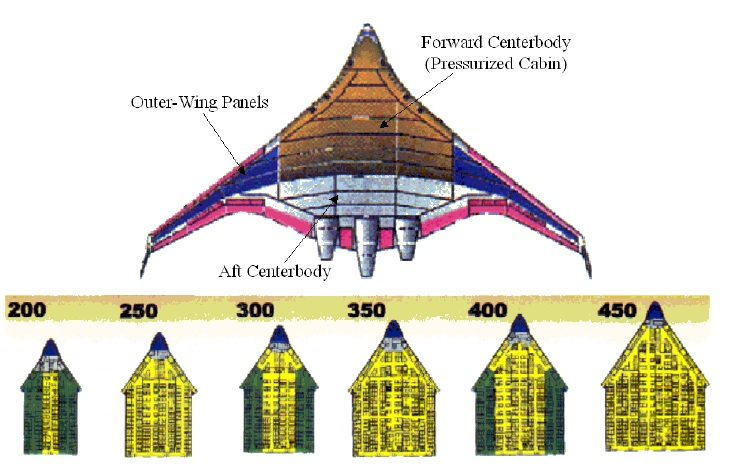
\includegraphics[keepaspectratio, width=0.6\textwidth]{images/chap1/bwb_bradley_concept.jpg}
	\caption{Blended Wing-Body cabin design, according to Bradley~\cite{bib:bradley_bwb}}
	\label{fig:bwb_bradley_concept}
\end{figure}
The concept for the cabin is the integrated one: he assumed that the cabin is divided into bays by the ribs, and each bay can allocate a single aisle with two column of passengers.
Then, he built the models and ran FEM analyses, for different configurations, to estimate the cabin mass. 
With the data obtained, he aimed to find a surrogate model, where the cabin mass formula takes the following shape:
\begin{equation}
	\label{eq:cabin_mass_general}
	m_{cabin} = a\left(m_{TO}\right)^b\left(S_{cabin}\right)^c
\end{equation}
where $m_{cabin}$ is the mass of the cabin, $m_{TO}$ the maximum takeoff weight, $S_{cabin}$ the cabin surface and $a$, $b$, $c$ some constants to be determined. 

Using the regression analysis, the three constants may be determined, finally having
\begin{equation}
	\label{eq:bwb_cabin_mass}
	m_{cabin} = k_s 0.316422 \left(m_{TO}\right)^{0.166552}\left(S_{cabin}\right)^{1.061158}
\end{equation}
where $k_s$ is a scaling factor to consider different technologies, that in his work was calibrated on the Boeing data, resulting to be $k_s=5.698865$. 
This model has then been implemented into FLOPS, a NASA in-house code for the preliminary design, to size a BWB, but as already said it has been abandoned and no further development came out. 

The main limiting factor of the model proposed by Bradley is that it uses very aggressive hypothesis on the composite material, and it considers also one load case, with reference values from Liebeck~\cite{bib:liebeck_2004}; also, it does not consider the effect of the cabin thickness. 
Despite these drawbacks, it has been successfully applied in other projects~\cite{bib:liu} and still remains a good starting point for further development of a conceptual tool for the BWB.

Some authors carried out also a dynamic structural analysis for the BWB, in order to capture the vibration modes~\cite{bib:yingsong, bib:weihua, bib:stroscher, bib:carlsson}.
Despite the research on this field is very limited, results show that a BWB configuration suffers less of flutter problem, due to stiffer structure, but torsional and bending moment are more critical. 
The most complete work is the one presented by Stettner and Voss~\cite{bib:stettner}, who included also handling qualities together with aeroelasticity analysis, showing that the trim problem is not trivial. 
Their main conclusion is that the BWB configuration needs more control surfaces than conventional aircraft to ensure stability and controllability, especially at low speed condition, where the bending and torsional moments are more relevant. 

\subsubsection{Aerodynamics tradeoff for the Blended Wing-Body}
\label{subsubsec:chap1_bwb_aero}

The BWB design is mainly done for improving aerodynamics performances, achieved by having a single lifting body and a reduced wetted area~\cite{bib:liebeck_1998}. 
The airfoil design is then a priority for the aerodynamics design, in particular for the cabin section, in which the thickness has to be large enough to allocate the passengers. 

The BWB design is highly influenced by equilibrium and stability constraints: for longitudinal equilibrium, the center of gravity should be afterwards the aerodynamics center~\cite{bib:anderson_perfo}, but this positioning implies statically unstable aircraft.
Herein, classical notation for aircraft stability is considered: momentum is positive when it is clockwise~\cite{bib:roskam_perfo, bib:roskam_flight_dynamics}. 
In conventional aircraft an horizontal tail is designed to make the aircraft stable, but being the BWB a tailless concept, there are no elements for trim. 
The goal is to have a small positive momentum coefficient around the center of gravity $C_{M_{cg}}$, at limit zero, which represents the best condition. 
Most of the airfoils, instead, are designed to obtain a negative $C_m$~\cite{bib:abbott}, the only exception is represented by the reflex airfoil. 
These types of airfoils have a trailing edge camber line lifter upward, generating a positive $C_m$, and this effect makes them perfect for the BWB design~\cite{bib:alex, bib:wang}.
The most common reflex airfoil family is represented by the NACA 5-digit series~\cite{bib:abbott}, but other families have been developed, like the MH family, deputed for the use on tailless aircraft~\cite{bib:mh_airfoiltool, bib:eppler}. 

However, using a reflex airfoil could compromise the transonic behaviour~\cite{bib:sargeant}: due to three-dimensionality, most of the centerbody lift is generated at the front.
For a reflex airfoil, this zone needs more curvature to counteract the loose of lift in the afterward part. 
As such, the critical and drag divergence Mach numbers are lower than that of a conventional airfoil, with potentially issue in the transonic regime. 
To limit the contribution to compressibility, as general rule, the thickness-to-chord ratio for the centerbody must not exceed 18\%~\cite{bib:kozek, bib:ikeda}.

The path just described helps the section design, but on a global point of view the aerodynamics load and the target $C_l$ distribution drive the design~\cite{bib:anderson_perfo}. 
It is to recall that the aerodynamics load is a punctual quantity, associated to the lift distribution as follow
\begin{equation}
	\label{eq:aero_load}
	\gamma\left(\eta\right) = \frac{c\left(\eta\right)C_l\left(\eta\right)}{2b}
\end{equation}
where $\eta=\frac{y}{\frac{b}{2}}$ is the non dimensional coordinate in the spanwise direction, $c$ and $C_l$ the local chord and lift coefficient, and $b$ the wing span. 
Integrating this quantity over the span the global $C_L$ is obtained
\begin{equation}
	\label{eq:global_cl_aero_load}
	C_L=AR\int_{0}^{\frac{b}{2}}\gamma\left(\eta\right)d\eta
\end{equation}
with $AR$ being the aspect ratio. 

On a conventional aircraft, with an aspect ratio above 5-6, the Prandtl theory gives results with a good accuracy; the reduced aspect ratio of the BWB, however, suggests that the Prandtl theory is not valid anymore, but the Jones theory may be more indicated~\cite{bib:cdn_notes}. 
This theory states that, in case of a low and untwisted aspect ratio wing, the aerodynamics load follows the elliptical distribution, and then from one hand the induced drag is minimised, but from the other hand it shows high $C_l$ at the wing tip for untwisted configuration, with consequently issues for the transonic performance and controllability because of the impossibility to use ailerons. 
Qin et al.~\cite{bib:qin} studied the load distribution on a BWB configuration, using RANS methods, and confirmed that the elliptical distribution is obtained with an untwisted wing. 
To balance the induced drag and the transonic performance, they added a twist distribution, using the inverse design technique, and found that the best load is obtained averaging and elliptical load with a triangular one. 
The inverse design is done using a low fidelity method (panel method); the results are then assessed on a set of points with high fidelity (RANS method).
Their results are presented in Fig.~\ref{fig:qin_cl_target} and Fig.~\ref{fig:qin_load_target}, as well as in Table~\ref{tab:qin_load_results}. 
With the average load, the lift coefficient at the tip is not as high as the elliptical case, avoiding stall and compressibility problems, but it is not as low as the triangular distribution, avoiding to increase the angle of attack to find the right lift. The elliptical-triangular distribution has a lower global $C_L$, but the difference is small (around 2\%); from Table~\ref{tab:qin_load_results} it can also be noted that, even if for an elliptical distribution the induced drag is lower, the wave drag is instead higher and in the end the global $C_D$ is higher, confirming that it is not the global optimal distribution, but only with respect to the induced drag. 
\begin{figure}[!h]
	\centering
	\begin{subfigure}{0.5\textwidth}
		\centering
		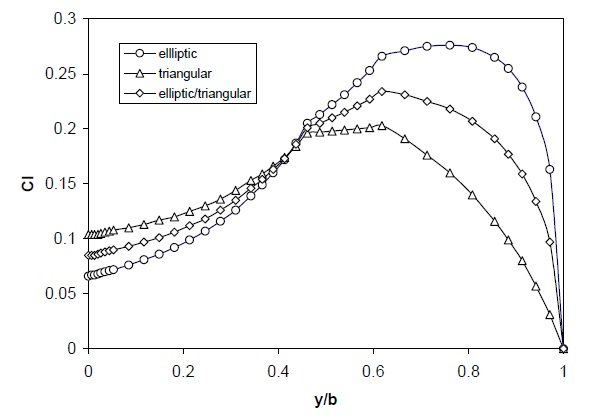
\includegraphics[keepaspectratio, width=\linewidth]{images/chap1/cl_target.jpg}
		\caption{Target lift distribution as a function of non dimensional span, for the case examinated by Qin et al.~\cite{bib:qin}.}
		\label{fig:qin_cl_target}
	\end{subfigure}
	\begin{subfigure}{0.5\textwidth}
		\centering
		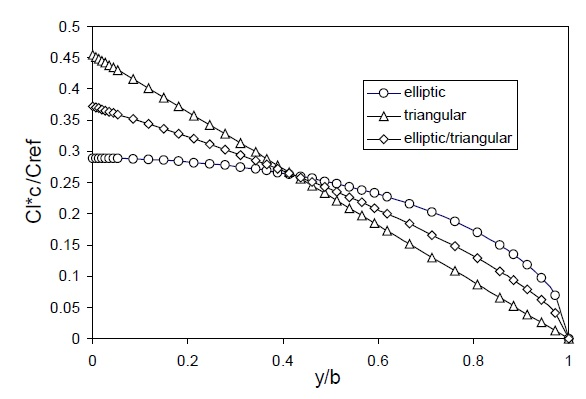
\includegraphics[keepaspectratio, width=\linewidth]{images/chap1/load_target.jpg}
		\caption{Target aerodynamics load distribution as a function of non dimensional span, for the case examinated by Qin et al.~\cite{bib:qin}.}
		\label{fig:qin_load_target}
	\end{subfigure}
	\caption{Aerodynamics tradeoff for a BWB, from the work of Qin et al.~\cite{bib:qin}.}
	\label{fig:qin_results}
\end{figure}

\begin{table}[!h]
	\centering
	\caption{Comparison of performance for the different target distributions examinated in the work of Qin et al.~\cite{bib:qin}, related to a BWB configuration.}
	\begin{tabular}{l l l l l l}
		\hline
		{Twist distribution}  & {$C_L$} & {$C_{D}$} & {$C_{D_{i}}$} & {$C_{D_{f}}$} & {$C_{D_{w}}$} \\
		\hline
		Baseline     & 0.4136 & 0.03268 & 0.02504 & 0.00764 & 0.00407 \\
		Elliptic     & 0.4102 & 0.02837 & 0.02031 & 0.00806 & 0.00209 \\
		Averaged     & 0.4090 & 0.02783 & 0.02008 & 0.00774 & 0.00180 \\
		Triangular   & 0.4071 & 0.02866 & 0.02083 & 0.00783 & 0.00161 \\
		\hline
	\end{tabular}
	\label{tab:qin_load_results}
\end{table} 

The work just described is interesting for two main reasons: it confirms that the Jones theory can be applied on a BWB, and it is the first evidence of a strategy in which the low fidelity is used to design a BWB, with the results being lately assessed using high fidelity. 
For what has been extensively said in Section~\ref{sec:chap1_ac_design_cycle}, at conceptual design is a key point to have fast and reliable methods, and Qin suggested a first path to follow in the conceptual aerodynamics design of the BWB. 

Beside this work, the other major references about the BWB aerodynamics used RANS method for the design: the design point is chosen, based on the target $C_L$, and then the configuration is resized until it matches the requirement.
This approach has the drawback that there are no information about the other operating points at which the BWB flies~\cite{bib:li_bwb}.
 
In the past year, fostered in the progress made in the MDO techniques~\cite{bib:martins_mdo}, different authors used optimisation algorithm for the geometry design, included the airfoil.
The first ones were Mader and Martins~\cite{bib:mader}, who tested on a flying wing this approach. 
Later Lyu and Martins set up an optimisation routine for a BWB, based again on a RANS solver~\cite{bib:lyu}. 
They defined a total of 273 design variables, regarding the twist distribution, the airfoil shape, the local sweep and chord, and the span, as shown in Fig.~\ref{fig:lyu_bwb_dv}. 
They investigated the impact of the various constraints and design variables on optimised BWB: trim and static stability were investigated both for the design and off design conditions. As a result, it was possible to find the best combination of wing twist and airfoil reflex to maximize the efficiency, satisfying at the same time trim and stability constraints.
\begin{figure}[h!]
	\centering
	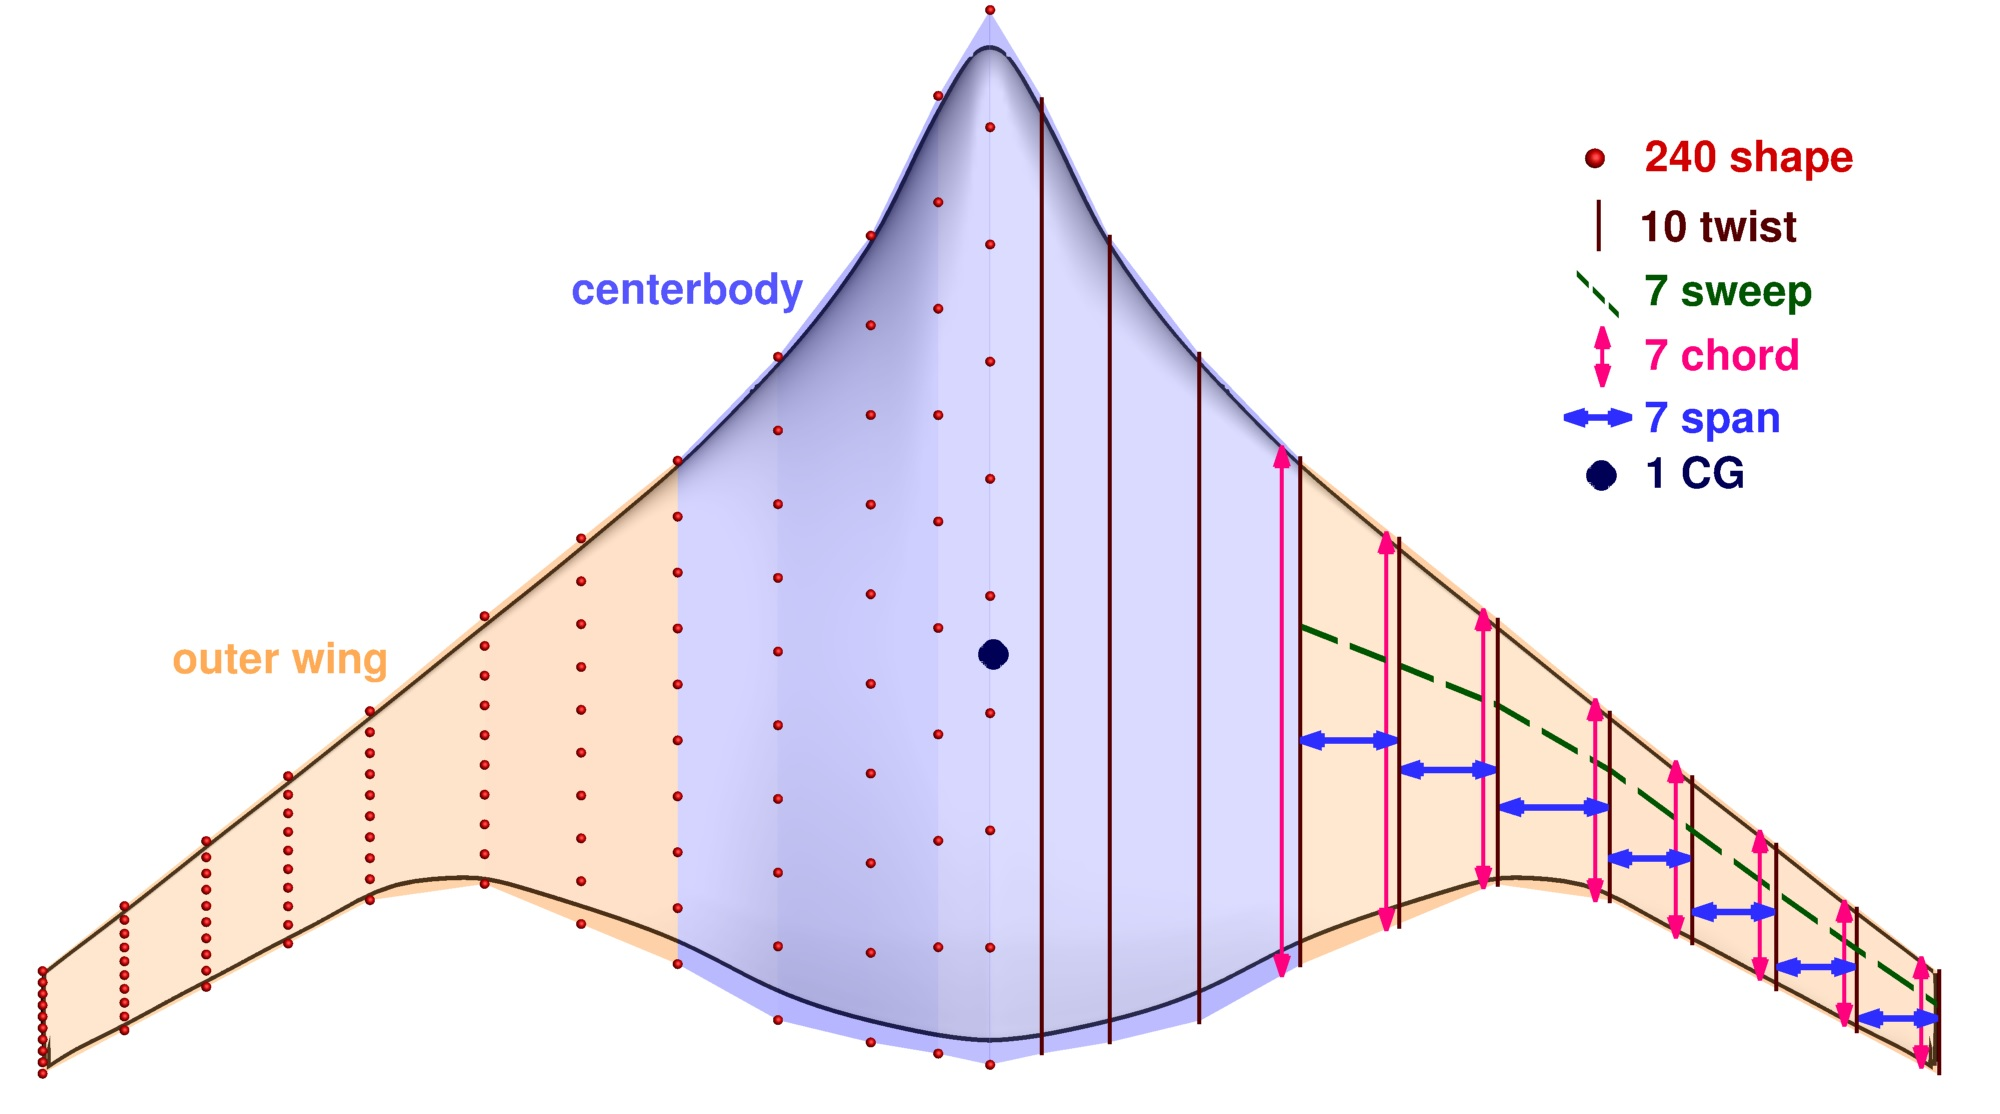
\includegraphics[keepaspectratio, width=0.8\textwidth]{images/chap1/bwb_martins_design.jpg}
	\caption{Shape and planform design variables considered in the work of Lyu and Martins, for the BWB optimisation~\cite{bib:lyu}. }
	\label{fig:lyu_bwb_dv}
\end{figure}

Liou et al.~\cite{bib:liou_2016, bib:liou_2017} carried out a similar work, including also the engine integration within the airframe, on a NASA hybrid configuration. 
Through all these works, that do not cover all the bibliography for the subject, the RANS-based aerodynamics shape optimisation method has been well assessed: they demonstrated that is a pratical tool for the BWB aerodynamics design. 
The main drawback is the computational cost: it is unfeasible to carry out such simulations on a single processor, and then a multiprocessor architecture is needed; still, the computational cost remains high. 
As example, in the work of Lyu and Martins~\cite{bib:lyu}, a single optimisation converged in 10~\si{\hour} using 240 processors. 
Thus, it is unfeasible to integrate CFD analysis for aerodynamics within the conceptual design loop, but it can be used to validate low fidelity methods or to define surrogate models, based on few set of geometrical parameters. 

On this direction, a first step has been done by Prince et al.~\cite{bib:prince}, who tested a commercial code, based on panel method, and compared the results with a RANS solver: they reports a maximum error of 10\% for the BWB configuration, which may be acceptable at conceptual design. 
Also, the maximum difference occurs at very high Mach number, when the compressibility effects are dominating the flow field; at low Mach numbers the agreement between the methods is much more marked. 

This work and the already mentioned work of Qin et al. represent the two most interesting cases in which theory or low fidelity methods are applied for the BWB configuration; further investigation is needed to get more reliable results, or even surrogate models to replace the empirical equations suggested by Roskam and extensively used for conventional aircraft~\cite{bib:roskam_partVI}.

The overview on the BWB concept ends up here: the next paragraph will discuss the possible integration among the innovative technologies identified to finally converge towards a potential solution capable to match environmental goals. 

\section{The research problem} 
\label{sec:chap1_research_problem}

\subsection{Towards a promising solution for aviation sustainabilityn}
\label{subsec:chap1_conf_proposition}

The previous section reports a review of the most promising innovative technologies considered in literature, to match the aviation's environmental goal for the upcoming years. 
Among all the possibilities, the hybrid and electric propulsion has been taken into account: from the studies reported came out that this technology has been identified as the best choice for the next generation aircraft. 
In particular, the main feature is that it opens new and still unexplored possibilities, \textit{e.g.} the integration with a BLI device to improve aerodynamics. 
Distributed propulsion is identified as a solution to take advantage of the hybrid propulsion, especially because DEP enhances the benefits coming from the BLI, and viceversa. 

Then, the focus has been shifted on the best architecture for this integration: in fact, BLI to be efficient requires large chords, otherwise its impact is negligeable. 
The solution is the Blended Wing-Body architecture, which is characterised by the integration of aerodynamic, structure and payload. 
By definition, the BWB is a whole lifting surface, and offers very large chords. 
So, it comes almost naturally to consider the Blended Wing-Body featuring distributed electric propulsion as possible solution for next generation aircraft. 
In fact, it takes advantages from all the innovative aspects described above. 
It is to note that innovation is brought on a two different level: propulsive, with the introduction of a new power plant, and structural, with a disruptive concept mainly designed for high aerodynamics performances. 

The intuition of BWB with DEP is confirmed by one of the most known concept proposed by NASA, within the N+3 program: the N3-X turboelectric concept~\cite{bib:kim_n3x_2008}. 
This concept, shown in Fig.~\ref{fig:nasa_n3x}, has been designed to be competitor of the Boeing 777 in terms of range and payload, and it is characterised by the integration of a distributed electric propulsive system within the BWB architecture. 
The entry into service goal is set to 2040: technological assumptions are made in perspectives for this horizon. 
\begin{figure}[!h]
	\centering
	\includegraphics[keepaspectratio, width=0.6\textwidth]{images/chap1/nasa_n3x.jpg}
	\caption{NASA N3-X concept~\cite{bib:kim_n3x_2008}.}
	\label{fig:nasa_n3x}
\end{figure}
The propulsors are mounted at the trailing edge, with the electric power coming from two generators, located at the wing tip; studies from Kim et al.~\cite{bib:kim_2013} show that this configuration enables very high propulsive efficiency, thanks to the partial electrification of the engine's cycle. 
The N3-X has been presented for the first time in 2008: both Kim~\cite{bib:kim_n3x_2008} and Felder~\cite{bib:felder_2009} performed preliminary studies to have a first estimation of its performance. 
Both the works showed that N3-X offers very good performance in terms of fuel reduction; as a consequence, deeper studies were conducted to confirm the preliminary results~\cite{bib:felder_2012, bib:kim_n3x_2014}, with refined trade-off for the weights~\cite{bib:brown_n3x}, noise and emission~\cite{bib:berton}. 
It has been estimated that the concept requires an amount of power in the order of 50~\si{\mega\watt}: such demand makes the superconducting technology and the associated cryogenic subsystems the only possible way to satisfy the requirements. 
In different works Rolls-Royce and the University of Strathclyde in UK collaborated on electrical system trades~\cite{bib:armstrong_n3x_2012, bib:armstrong_n3x, bib:armstrong} and the system safety analysis of such a complex architecture~\cite{bib:ross, bib:shaw_2014, bib:shaw_2015}. The assessment of performance shows a reduction of 70\% in fuel burn, compared to the Boeing 777~\cite{bib:felder_2011}, due to the partial electrification and the improved airframe; economic viability is demonstrated too~\cite{bib:goldberg}. 
The main issue with this concept is that it uses a very aggressive technology, and thus it introduces a large amount of technological risk for an EIS2040: Jansen et al.~\cite{bib:jansen} studied, for this case, the required individual technology for the electric subsystems, and they are really challenging even dealing with such a large technological horizon. 
Despite that, the N3-X is still a milestone for the integration of the hybrid propulsion within BWB airframe and the benchmarking for the fuel burn, noise and emission reduction. 

Beside the N3-X, other authors found an interest in the BWB featuring hybrid propulsion: Rodriguez presented the benefits coming from the BLI on a reference Boeing geometry~\cite{bib:rodriguez}, meanwhile Kok~\cite{bib:kok} and Campbell~\cite{bib:campbell_bli} separately studied the effects of combining DEP and BLI on a BWB configuration.
Finally, Ko et al.~\cite{bib:ko_bwb} set up a multidisciplinary optimisation formulation to get the optimal geometry with respect to the propulsive benefits. 
All these works report an improvement in the fuel efficiency above the 20-30\%.

So far, the N3-X is the most complete concept, but it has been studied considering individual disciplines, with specific high fidelity tools, but no OAD process is defined. 
Also, it is competitor of the Boeing 777, so it is designed for long range and 450 passengers, whereas the single aisle aircraft, as \textit{i.e.} the Airbus A320, represents the critical segment for emission (see Fig.~\ref{fig:aviation_emission_breakdown}), and in Boeing perspective it will be the segment with the major growing ratio~\cite{bib:boeing_outlook_market}. 

\subsection{Problem statement and proposed solutions}
\label{subsec:chap1_prob_statement}

This research, finally, has the objective to define an OAD process, at conceptual level, for the study of a BWB featuring DEP, in the same segment as the Airbus A320 (short/medium range, 150 passengers). 
An EIS 2035 is considered; to limit the risk associated to the concept, only non-cryogenic technology is considered. 
In fact, there is a lot of uncertainty about the cryogenic technology and its application for aviation on short term. 

The research problem can be summed up in the following question: 
\begin{mdframed}[hidealllines=true,backgroundcolor=green!20]
	\textbf{Research problem.} How will the conceptual design process can be revised for the study of an unconventional configuration that features an innovative hybrid powerplant?
\end{mdframed}
The answer is not obvious: conceptual design methods, described in Sec.~\ref{sec:chap1_ac_design_cycle}, are well assessed for a TAW aircraft configuration, but are not valid anymore for hybrid aircraft. 
The example of the N3-X, as well as the X-57, the STARC-ABL and others presented in Sec.~\ref{sec:chap1_key_innovative_techno}, show hybrid/electric aircraft have more interaction between disciplines than a conventional aircraft. 
As already remarked, even the Breguet equation does not hold yet and must be revised~\cite{bib:hepperle, bib:marwa}. 
The most representative case of the existing coupling is provided by aerodynamics and propulsion, that cannot be considered as separated disciplines, since each one impacts the other one. 
Pornet et al.~\cite{bib:pornet, bib:pornet_2014} presented a preliminary sizing procedure for hybrid aircraft, and they stressed in different points that integration of a new hybrid powerplant has an impact on all disciplines.
At that stage several assumptions have been done, that limit the application.  
Cinar et al.~\cite{bib:cinar_sizing} arrived at same conclusion; De Vries et al.~\cite{bib:devries_2018} presented instead a revised procedure for the sizing that includes aero-propulsive interaction, demonstrating on a test case of regional aircraft that the two disciplines cannot be considered separated anymore. 

More complications come considering the thermal management, which has been neglected in the three works cited above~\Cite{bib:pornet, bib:cinar_sizing, bib:devries_2018}: Freeman~\cite{bib:freeman} and Campbell~\cite{bib:campbell_prop} noted that thermal aspects cannot be neglected when considering electric architecture. 
Due to the large demand of power, dissipation due to Joule effect is significant, and cooling systems must be included to avoid problems related to structure's heating. 

A key point, addressed by Brelje and Martins, is that the classical design procedure relies on MDA, and its capability to deal with the problem of unconventional configurations is limited~\cite{bib:brelje_biblio}.
Research must focus more on a revised sizing procedure, based on Multidisciplinary Design optimisation (MDO)~\cite{bib:martins_mdo}; sometimes the notation MDAO (Multidisciplinary Design Analysis and Optimisation) is used to highlight the multidisciplinarity characterization. 
The MDAO, as defined by Martins and Lambe~\cite{bib:martins_mdo}, is a ``field of engineering that focuses on the use of numerical optimization for the design of systems that involve a number of disciplines and subsystems''.
MDO origins can be traced back to '60 years, when Haftka~\cite{bib:haftka_1973, bib:haftka_1975, bib:haftka_1977, bib:haftka_1979} and Schmit~\cite{bib:schmit_1960, bib:schmit_1965, bib:schmit_1981, bib:schmit_1984} started to extend their experience in the structural optimisation to other disciplines. 
In recent years, thanks to the improvements in computational science and the new resources available, MDO is become a powerful tool for aircraft design~\cite{bib:kroo, bib:manning, bib:antoine, bib:henderson, bib:alonso} and other engineering problems~\cite{bib:martins_mdo}. 
Moreover, it is recognised as the only solution to deal with the problem of unconventional configurations~\cite{bib:lyu, bib:raymer, bib:brelje_biblio}. 
Brelje and Martins demonstrated their assumption on another work~\cite{bib:brelje_model}, whereas they present a MDO tool for the optimisation of small electric aircraft. 
Despite the limiting assumptions in models used, they concluded that performances were indeed improved compared to a conventional MDA procedure. 
Also, they identified the problem of a full MDO formulation for aircraft design problem as still an open issue in literature. 

Finally, the answer to the research problem comes out. 
It can be divided into three subpoints, as follow: 
\begin{mdframed}[hidealllines=true,backgroundcolor=green!20]
	\textbf{Answer to research problem.} 
	The problem of sizing unconventional configurations with hybrid architecture for the thrust generation at conceptual level can be tackled through:
	\begin{itemize}
		\item The definition of new models, to consider the impact of the innovative architecture on geometry, structure, aerodynamics and performance evaluation;
		
		\item The application of a multifidelity approach, to calibrate the conceptual design methods with more refined simulations;
		
		\item The definition of a sizing procedure based on Multidisciplinary Design Analysis and Optimisation, because of its capability to establish tradeoff taking into account all the interactions between disciplines, particularly relevant for unconventional aircraft. 
	\end{itemize} 
\end{mdframed}

The definition of a MDAO formulation opens two related issues: ``Which are the models to use for the discipline, to account for innovative configurations?'' and ``Which is the best MDO formulation for aircraft design problem?''.
All these issues will be addressed in the manuscript; the two main Ph.D. objectives can be summed up considering these points: 
\begin{itemize}
	
	\item Set up of a complete multidisciplinary design analysis process for the sizing of the innovative concept and its performance evaluation;
	
	\item Choice of the most suitable multidisciplinary design optimisation formulation, in order to carry out an optimisation loop.
\end{itemize} 

It has been noted several times, and recalled here, that the test case of BWB with DEP presents two main innovations, one related to the propulsive architecture and another one to the overall configuration. 
To facilitate the development of a sizing procedure, the work is divided into three minor steps:
\begin{itemize}
	\item Study of a TAW configuration featuring distributed electric propulsion,
	\item Study of a medium range BWB, with conventional engines,
	\item Merge of the two previous concepts, to finally arrive at the BWB with distributed electric propulsion.
\end{itemize}

The Ph.D. roadmap, that shows this division into intermediate steps, is shown in Fig.~\ref{fig:phd_roadmap}.
This way to proceed allows also to study the two innovative aspects introduced separately, assessing their benefits in terms of aircraft performance individually. 
\begin{figure}[!h]
	\centering
	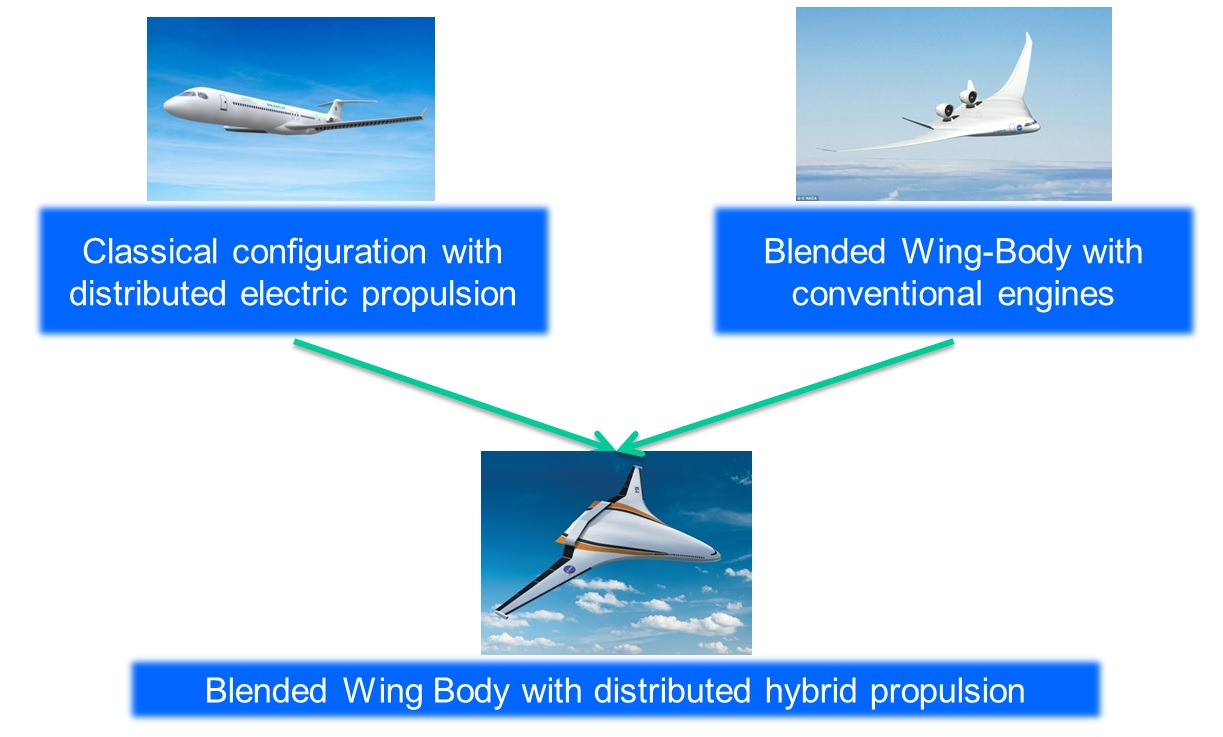
\includegraphics[keepaspectratio, width=\textwidth]{images/chap1/phd_roadmap.jpg}
	\caption{Ph.D. roadmap, representing the two separated steps to finally converge toward the Blended Wing-Body with distributed electric propulsion configuration.}
	\label{fig:phd_roadmap}
\end{figure}

\clearpage

\begin{mdframed}[hidealllines=true,backgroundcolor=blue!20]
	\section*{Synthesis of the chapter}
	
	\begin{itemize}
		\item Increase of emission poses a problem for aviation: to reduce the environmental footprint, a disruptive concept must be introduced. 
		
		\item The exploration of an innovative concept must be carried out at conceptual design level. 
		
		\item Key technologies to match the enviromental goals are explored:
			\begin{itemize}
				
				\item[-] Hybrid and electric propulsion offers new and still unexplored features. 
				
				\item[-] Blended Wing-Body is identified as the most promising architecture for the integration with a distributed electric propulsion system.
				
				\item[-] Blended Wing-Body with distributed electric propulsion is chosen as test case for the research.
				
			\end{itemize}
		
		\item Because of the strong integration among disciplines for unconventional aircraft, classical conceptual design loop based on Multidisciplinary Design Analysis may lead to misleading results: definition of an Overall Aircraft Design procedure based on Multidisciplinary Design Optimisation technique is investigated. 
		
		\item The two key technologies introduced (hybrid propulsion and BWB architecture) are studied separately: final concept results from the merging between the two. 
	\end{itemize}
\end{mdframed}
%2-FAST development for conventional aircraft
\chapter{Development of an optimisation framework for conceptual aircraft design}
\markboth{Development of an optimisation framework for conceptual aircraft design}{Development of an optimisation framework for conceptual aircraft design}
\label{chap2:fast_base_mdo}

%\begin{mdframed}[hidealllines=true,backgroundcolor=lightgray!20]
%	\section*{Résumé}
%	Ce chapitre présente l’élaboration d’un cadre pour le dimensionnement et l’optimisation d’un avion de grande capacité. 
%	Le code développé repose sur l'intégration de FAST dans la plate-forme d'optimisation multidisciplinaire OpenMDAO.
%	
%	FAST est un outil d'analyse de conception multidisciplinaire développé par l'ONERA et l'ISAE-Supaero pour le dimensionnement d'aéronefs conventionnels. 
%	Entièrement écrit en Python, il est basé sur les méthodes classiques du manuel de conception et sur une approche de masse ponctuelle pour l’estimation des performances. 
%	La boucle de dimensionnement regroupe toutes les disciplines clés de la conception des aéronefs: aérodynamique, structure/masse, propulsion, performances, ainsi que certains aspects liés aux spécifications de certification. 
%	Le scénario de test de validation de FAST est l’avion CERAS d’Airbus A320.
%	
%	OpenMDAO est plutôt une plate-forme d'optimisation multidisciplinaire développée par la NASA Glenn Research Center. 
%	Ce intègre une grande variété d'algorithmes d'optimisation, déjà inclus dans les bibliothèques Python, dans un code créé spécifiquement pour faciliter la définition de problèmes d'optimisation de conception multidisciplinaire. 
%	Grâce à sa logique, composée de modules indépendants, le problème peut être décomposé et organisé au plus haut niveau très facilement~: cette approche modulaire permet de remplacer certaines disciplines avec des modifications mineures. 
%	La principale caractéristique d'OpenMDAO est liée à MAUD, qui constitue un moyen innovant de calculer des dérivés pour résoudre des problèmes d'optimisation. 
%	Grâce à MAUD, OpenMDAO peut calculer efficacement les dérivées, en réduisant le coût de calcul, et il est principalement adapté aux optimisations basées sur les gradients. 
%	Son succès est attesté par la grande variété de travaux faisant appel à OpenMDAO que ce soit dans le cadre de problèmes aéronautiques et aérospatiaux ou d’autres sujets.
%	
%	Pour intégrer FAST dans OpenMDAO, le code doit être modifié et réorganisé: les anciennes disciplines sont décomposées en différents modules~; pour faciliter l'utilisation du gradient, chaque module correspond à une équation. 
%	À un niveau supérieur, les critères de conception, par exemple pour les surfaces d'aile et d’empennage, sont remplacés par la définition de contraintes de conception pour le problème d'optimisation, afin de permettre à l'optimiseur de trouver la meilleure solution dans l'espace de conception. 
%	Grâce aux méthodes numériques efficaces et à la logique d'OpenMDAO, le coût de calcul a été réduit de 5 minutes à environ 30 secondes pour une seule itération. 
%	Cependant, il présente l’inconvénient que la modularité a introduit 200 nouvelles fonctions, au lieu des 20 fonctions utilisés précedemment 20, ce qui peut compliquer la compréhension du code par un nouvel utilisateur.
%	La formulation résultante de l'optimisation multidisciplinaire est l’architecture MDF, qui apparaît comme la plus appropriée au problème de conception d'aéronef, bien qu'elle nécessite la définition d'une boucle complète d'analyse de conception multidisciplinaire.
%
%	La version intégrée a été appliquée sur le scénario du cas test CERAS: les résultats montrent que l'optimisation entraîne une réduction de la consommation de carburant d'environ 10\%, ce qui n'est pas négligeable en pourcentage.
%	Ensuite, l’avion CERAS est redimensionné en tenant compte de différentes plages de conception et d’hypothèses technologiques pour l’horizon 2035, afin d’obtenir un ensemble d’aéronefs de référence à utiliser pour la comparaison avec les configurations non conventionnelles qui seront proposées dans les chapitres suivants.
%	
%	Il est à mentionner que le travail d'intégration a été effectué en collaboration avec le MDO Lab. à l'Université du Michigan, lors d'une visite de 3 mois de janvier à avril 2018, avec le support financier de la Formaction Doctorale ISAE-Supaero.
%\end{mdframed}
%
%\cleardoublepage

\minitoc

\clearpage

\begin{mdframed}[hidealllines=true,backgroundcolor=purple!20]
	\section*{Outline}
	
	\begin{itemize}
	
		\item Description of FAST, the ONERA and ISAE-Supaero aircraft sizing tool, is given. 
		
		\item OpenMDAO, the multidisciplinary optimisation tool from NASA Glenn Research Centre, is presented. Notions on its logic are given, to understand the development of MDO problems. 
		
		\item An integrated sizing tool is obtained from the coding of FAST within the OpenMDAO platform. 
		
		\item The integrated code FAST and OpenMDAO is used to optimise the Airbus A320 CERAS test case. 
		
	\end{itemize}

\end{mdframed}

\cleardoublepage

\section{Introduction}
\label{sec:chap2_intro}

This chapter presents the sizing tool developed in this research to obtain a MDO procedure, considering the test case of a conventional aircraft. 
It comes from the integration of FAST~\cite{bib:fast_main}, an in-house code developed at ONERA and ISAE-Supaero, into OpenMDAO, an optimisation platform developed at NASA Langley Research Centre~\cite{bib:openmdao_website, bib:gray_omdao}. 

At first, Sec.~\ref{sec:chap2_fast_base_description} presents a description of the original code FAST, including discipline models and validation cases. 
Then, Sec.~\ref{sec:chap2_openmdao_overview} describes the multidisciplinary optimisation platform OpenMDAO, highlighting its capabilities and main features for optimisation problems.
Finally, the integration of FAST into OpenMDAO is reported in Sec.~\ref{sec:chap2_fast_omdao_base}, where the recoding work is detailed. 
This section gives also the chance to highlight differences between the MDA and the MDO approach, showing that the latest is more accurate when dealing with a large number of disciplines, thanks to the way the design constraints are defined. 
The new framework is then evaluated on the Airbus A320 CERAS test case~\cite{bib:ceras}, to assess the optimisation process, and is then used to define the reference aircraft, to compare with the hybrid and the BWB concept later. 

It must be mentioned that the work described in this chapter has been done in collaboration with the MDO Lab., at University of Michigan, during a visit conducted from January to April 2018.
The visit has been funded thanks to a grant for international exchange from \textit{Formation Doctorale} of ISAE-Supaero. 

\section{The sizing tool FAST}
\label{sec:chap2_fast_base_description}

\subsection{Overview}
\label{subsec:chap2_fast_overview}
FAST (Fixed-wing Aircraft Sizing Tool) is an in-house software, developed by ONERA and ISAE-Supaero, for aircraft sizing and analysis purposes~\cite{bib:fast_main}. 
Fully developed in Python 2.7, in its native version, it is a multidisciplinary code, capable to carry out the preliminary sizing of a turbofan aircraft, for given top level requirements (TLAR), and evaluate its performance.
The validation case is the A320 CERAS test case~\cite{bib:schmollgruber}, based on the Airbus A320 data~\cite{bib:a320_specifications}. 
During the process, it considers all the key disciplines in aircraft design: aerodynamics, structure/mass estimation and propulsion. 
Since FAST is tailored for the conceptual design, models are based mainly on semi-empirical equations, coming from classical design handbooks~\cite{bib:roskam_partI, bib:raymer} and Airbus experience and collected in the ISAE-Supaero notes~\cite{bib:airbus_notes}, which are accurate as long the conventional TAW configuration is considered. 

FAST interfaces also with other softwares, that are used for aerodynamics computation: XFOIL~\cite{bib:xfoil} for airfoil performance and OpenVSP~\cite{bib:openvsp} for the low speed polars. 
The last one is also used for visualisation purposes at the end of the sizing procedure. 
An \texttt{xml} file (eXtensible Markup Language) is used for the flow data: it containts the initial set of TLAR and collects the output variables of the design process. 
Thus the \texttt{xml} file is the I/O file for the FAST workflow.

After its first developments, FAST has been successfully used in several projects, and it is now been expanded to consider regional aircraft, ATR type~\cite{bib:bohari}, and to interface with a certification constraint module and full mission simulations~\cite{bib:schmollgruber, bib:schmollgruber_phd}. 
The next sections give an outlook to the main elements of FAST: Sec.~\ref{subsec:chap2_fast_xml_struc} describes I/O file structure, Sec.~\ref{subsec:chap2_fast_mod_desc} reports details of  a description of all the parts of the software, and Sec.~\ref{subsec:chap2_fast_test_case} reports the results for the validation test case.  

\subsection{I/O structure file}
\label{subsec:chap2_fast_xml_struc}

To manage the dataflow, FAST relies on an \texttt{xml} file. 
This format is mainly indicated for the management of a large data flow, since it facilitates the inputs and the outputs, and is well interfaced with Python, thanks to the dedicated libraries~\cite{bib:nagel_cpacs}. 

FAST uses GAMME for reading and writing~\cite{bib:bedouet}: it is a meta-model, capable to automatically create Python dictionaries from the \texttt{xml} file. 
It can also handle units and their conversion, which is an added feature of relevance in aircraft design, where input data can be given following different unit systems.

The main argument of \texttt{xml} file is called \texttt{Aircraft}. 
Then this argument is structured in nine subparts, on different levels (from input data to output per discipline), as follows:
\begin{itemize}
	\item \textbf{TLAR.} This section contains the top level requirements for the aircraft: aircraft type (large passenger, business jet, \textellipsis), range, number of passengers, approach speed, cruise Mach number and maximum allowable takeoff runway length.
	
	\item \textbf{Configuration.} This section contains the parameters used to define the configuration, such as engine location or empennage type. Each of these specifications is identified by a numerical flag.
	
	\item \textbf{Mission.} This section contains the parameters to define the given mission, and, as outputs, the relative fuel breakdown, time of flight and takeoff/landing performances.
	This section has two sublevels: one related to the design mission, and another one to operational missions.
	
	\item \textbf{Cabin.} This section is used to define all the parameters for the internal cabin layout.
	
	\item \textbf{Geometry.} This section is dedicated to the geometry. 
	It is divided into several sublevels, one for each geometrical component: in each sublevel there are a few sets of inputs.
	As outputs, all the geometrical dimensions are reported. 
	This section is also shared with the OpenVSP visualisation tool, in order to create a 3D sketch of the aircraft at the end of the sizing loop.
	
	\item \textbf{Propulsion.} This section contains the input parameters for the engine definition, according to the chosen model, as it will be described later. 
	
	\item \textbf{Aerodynamics.} This section is solely for output, and it stores global aerodynamics parameters.
	
	\item \textbf{Weight.} This section is for the mass breakdown, and it is divided into sublevels: airframe, propulsion, secondary systems, furniture and crew. 
	The breakdown is made according to the standard defined by the French norm AR 2001/D~\cite{bib:mass_breakdown}.
	
	\item \textbf{Balance.} This section shows the same structure as the \texttt{Weight} section, but instead of masses it contains all the center of gravities positions, plus the global center of gravity. 
	It is also used to define the maximum allowable CG range variation, used to satisfy stability requirements.
\end{itemize}
An example of \texttt{xml} file structure is reported in Appendix~\ref{app:xml_file_struct}.

Accessing a file is a costly procedure in programming, even with dedicated libraries that facilitates the reading and writing: for this reason, FAST reads the \texttt{xml} file one time at the beginning of the process, to store all the input variables.
Afterwars, it accesses to the file again at the end of sizing, for output writing purposes. 

Finally, it must be highlighted that \texttt{xml} format has been largely used in aircraft design: a standard, called CPACS, is defined as common language, to facilitate the data sharing~\cite{bib:nagel_cpacs}. 
To enlarge the possible utilisation of the software, FAST is provided with a CPACS converter, to switch between this standard and the native \texttt{xml} standard for FAST. 

\subsection{Code description}
\label{subsec:chap2_fast_mod_desc}

The code is described in Fig.~\ref{fig:fast_basic}, with the xDSM standard, meanwhile the detailed algorithm (with the numbering referred to the figure) is reported below in Alg.~\ref{alg:fast_basic}. 
The scheme shown in Fig.~\ref{fig:fast_basic} highlights the multidisciplinary nature of the software: disciplines are connected each others and exchange lot of data, as indicated by the grey line. 
\begin{figure}[!h]
	\centering
	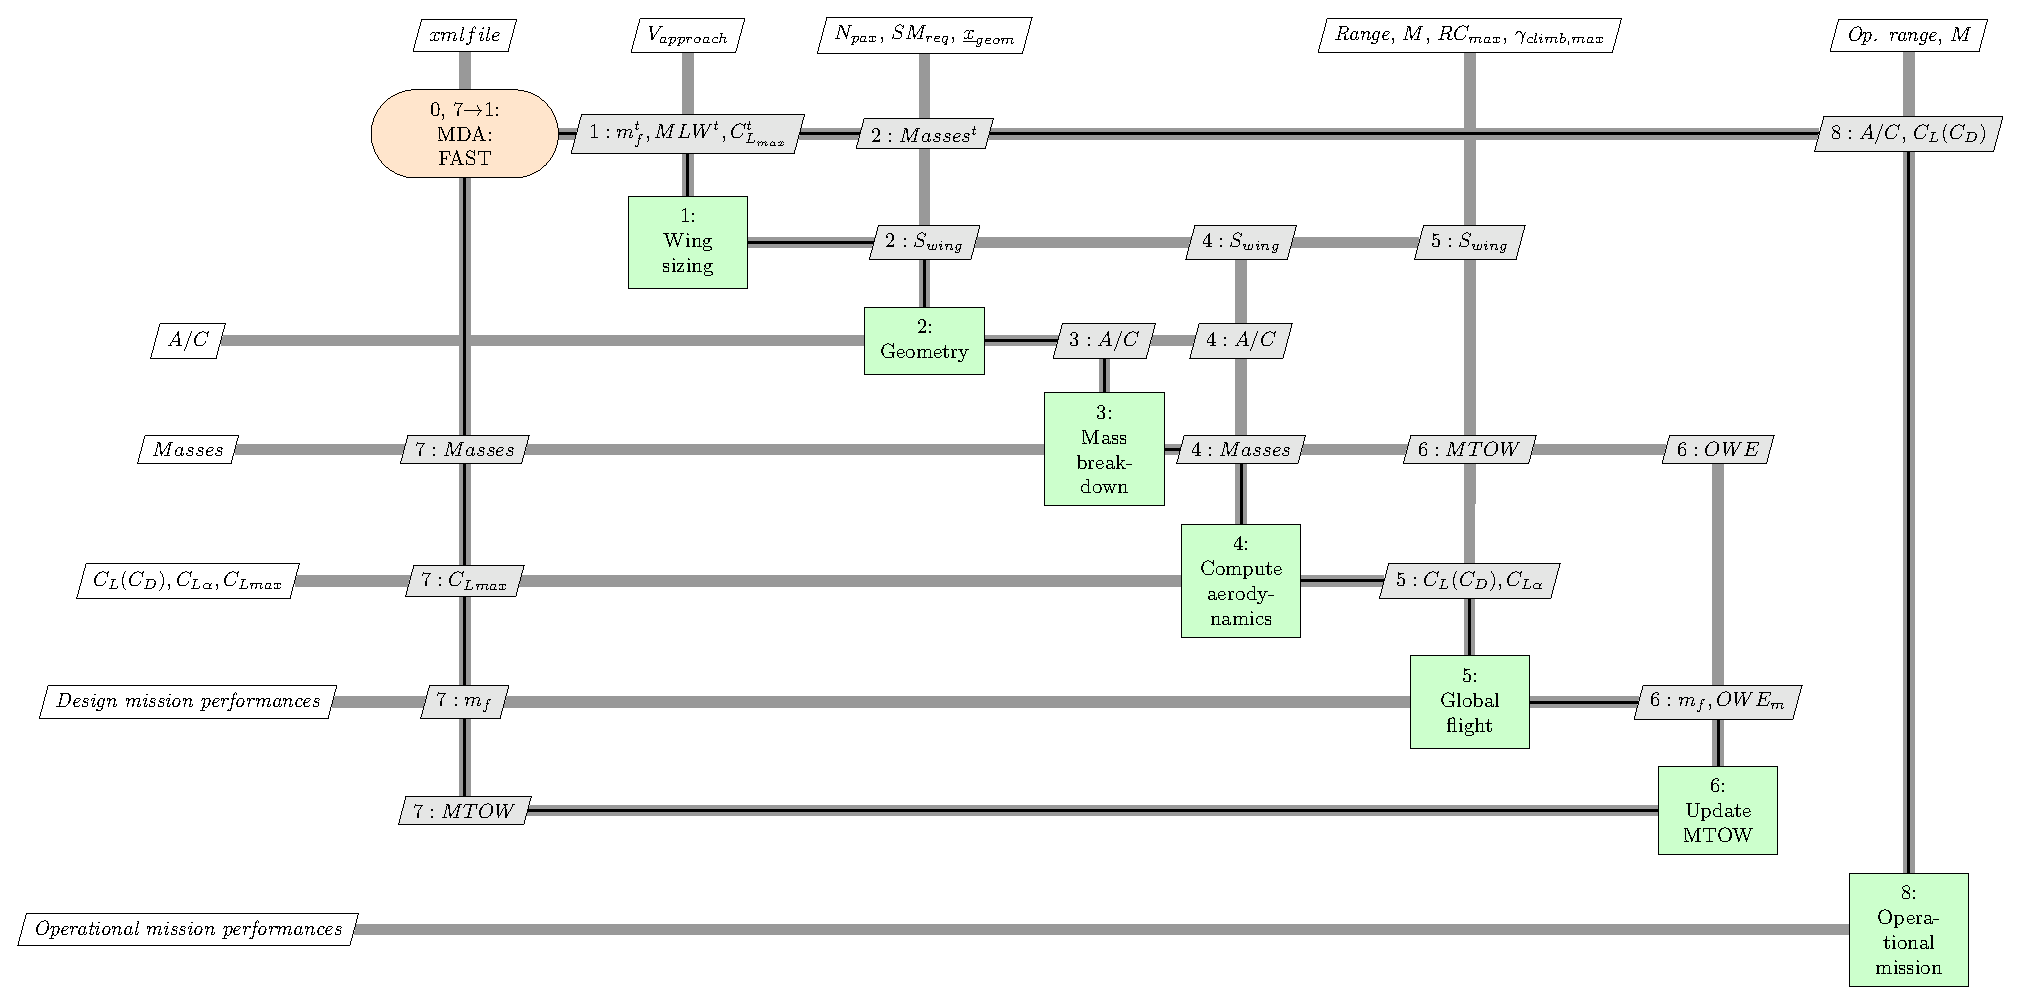
\includegraphics[keepaspectratio, width=1.2\textwidth, angle=90]{images/chap2/FAST}
	\caption{Diagram of FAST, using the xDSM standard~\cite{bib:lambe_xdsm}.}
	\label{fig:fast_basic}
\end{figure}

\begin{algorithm}[!h]
	\caption{FAST algorithm. Numbering is referred to diagram shown in Fig.~\ref{fig:fast_basic}.}
	\label{alg:fast_basic}
	\begin{algorithmic}
		\REQUIRE Initial design parameters (TLAR)
		\ENSURE Sized aircraft, drag polars, masses, design mission trajectory
		\STATE 0: Initialise the loop with a first estimate of geometry and masses, with the values from the \texttt{xml} file~\cite{bib:airbus_notes}. At this step engine is initialised too.
		\REPEAT
		\STATE 1: The wing area is obtained in order to supply enough lift in landing condition and to store all the fuel needed for the design mission.
		\STATE 2: The aircraft geometry is deduced through a resizing loop, to match the stability requirements.
		\STATE 3: Using the data coming from analysis 2, the masses and the center of gravities of each component are computed. Standard is the French norm AR 2001/D~\cite{bib:mass_breakdown}.
		\STATE 4: Aerodynamics analysis is carried out, to get the polars at low and high speed.
		\STATE 5: Performance calculation: the trajectory is performed through the integration of the flight equations using the Euler time step approach.
		\STATE 6: Update the value of MTOW, with the data coming from analyses 3 and 5.
		\STATE 7: Check the convergence: if the tolerance is below the needed threshold, return the sized aircraft, otherwise proceed to next iteration.
		\UNTIL {$7 \rightarrow 1$: MDA has converged}
		\STATE 8: Optionally, perform an operational mission, to assess the performance on different missions than the design one.
	\end{algorithmic}
\end{algorithm}

It must be noted that the engine is initialised outside the sizing loop, using the inputs from the \texttt{xml} file. 
The curves of thrust and specific fuel consumption SFC are obtained and provided to the performance analysis: in other words, FAST does not include the engine sizing in the design process.
Instead, it relies on a pre-existing engine deck, as will be detailed in Sec.~\ref{subsubsec:chap2_fast_propulsion}. 

The driven parameter for the MDA convergence is the operating weight empty OWE estimation.
There are two estimations for this parameter; the first one is obtained at analysis 3 as sum of all the airframe, propulsion, systems and furniture masses:
\begin{equation}
\label{eq:owe_struct}
m_{e_{3}} = \sum_{i=1}^{n}m_i
\end{equation}
where $i$ represents the generic component, as in the mass standard~\cite{bib:mass_breakdown}.

The second estimation is instead provided after the performance analysis:
\begin{equation}
\label{eq:owe_perf}
m_{e_{5}} = m_{TO} - m_f - m_{PL} 
\end{equation}

At convergence, the two values from Eq.~\eqref{eq:owe_struct} and Eq.~\eqref{eq:owe_perf} must be the same. 
The convergence criterion is then that the relative difference between the two does not exceed 0.05\%:
\begin{equation}
\label{eq:fast_conv_crit}
\left\lvert \frac{m_{e_{3}} - m_{e_{5}}}{m_{e_{3}}}\right\rvert \leq 5\times10^{-4}
\end{equation}
In case the error is above the value, MTOW is updated adding the difference between $m_{e_{3}}$ and $m_{e_{5}}$:
\begin{equation}
\label{eq:mtow_new}
m_{{TO}_{i+1}} = m_{{TO}_{i}} + \left(m_{e_{3}} - m_{e_{5}}\right)
\end{equation}

In next sections more details on the disciplinary analyses are provided. 
Indeed since they represent the starting point for the development aimed in this research, have a clear understanding of the models and their limit of validity is a key point.

\subsubsection{Propulsion}
\label{subsubsec:chap2_fast_propulsion}

In FAST the engine sizing is not included into the iterative process, but the curves representing its performances are provided to the code for the trajectory analysis. 
There are two engine's models that can be used in FAST: the first one is the engine deck used for the CERAS reference aircraft~\cite{bib:ceras}, meanwhile the second one is the so called ``rubber engine''~\cite{bib:roux}, which represents a model for the engine sizing, based on entries as thrust at sea level or BPR.

The CERAS engine is based on the deck used for the CERAS reference aircraft~\cite{bib:ceras}. 
The data are as close as possible to the Airbus A320's engine.
In particular, the by-pass ratio BPR is equal to 6 and the thrust at sea level is 117.8~\si{\kilo\newton}.  
The maps for thrust and fuel flow, as function of altitude and Mach, are provided to the performance module in FAST: according to the actual trajectory point, these parameters are evaluated through an interpolation. 
The maps are shown in Fig.~\ref{fig:ceras_engine_deck}.
The main limitation of this model is that thrust and fuel flow (then specific fuel consumption SFC too) are already provided, and there is no possibility to change the engine's parameters to obtain new curves. 
The field of application has been enlarged thanks to the definition of some corrective factors, that can be used to calibrate thrust and SFC; on top, this approach does not give any indication on the geometry data, so the impact on aerodynamics is neglected.
For a more detailed assessment a new model, that takes as input a set of engine parameters, must be defined.
\begin{figure}[!h]
	\centering
	\begin{subfigure}{0.45\textwidth}
		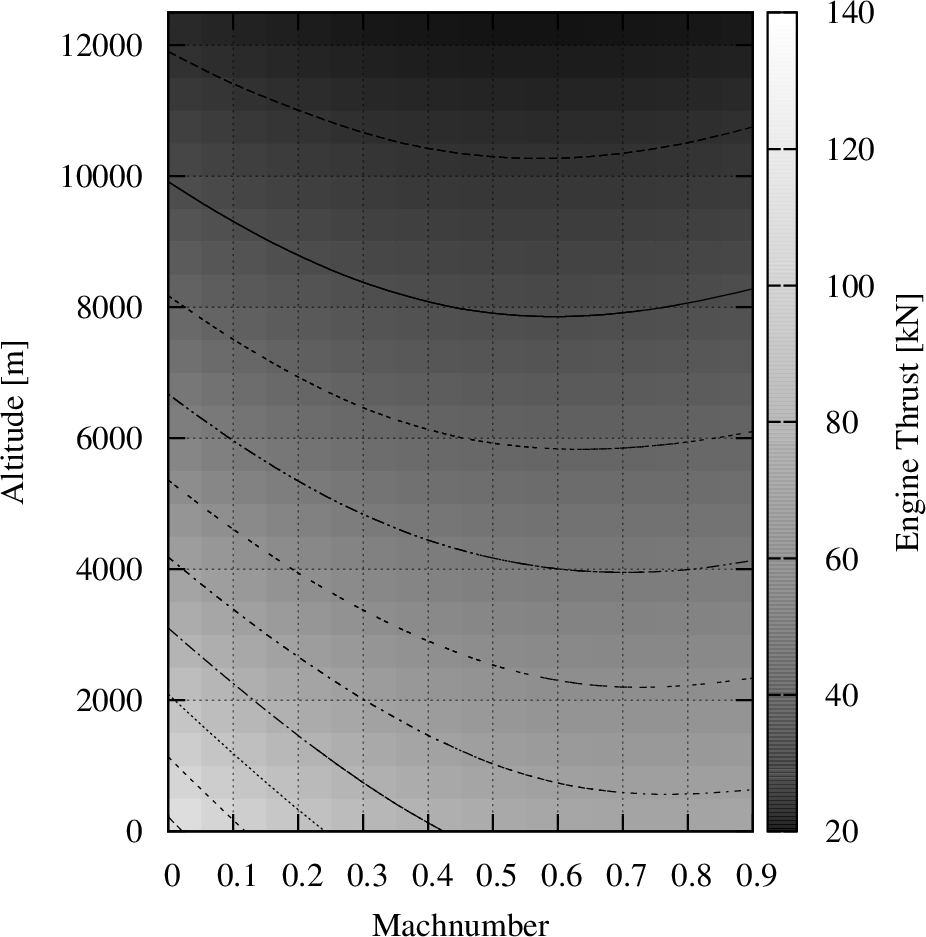
\includegraphics[keepaspectratio, width=\textwidth]{images/chap2/deck_thrust.png}
		\caption{Thrust data.}
		\label{subfig:ceras_thrust}	
	\end{subfigure}
	\begin{subfigure}{0.45\textwidth}
		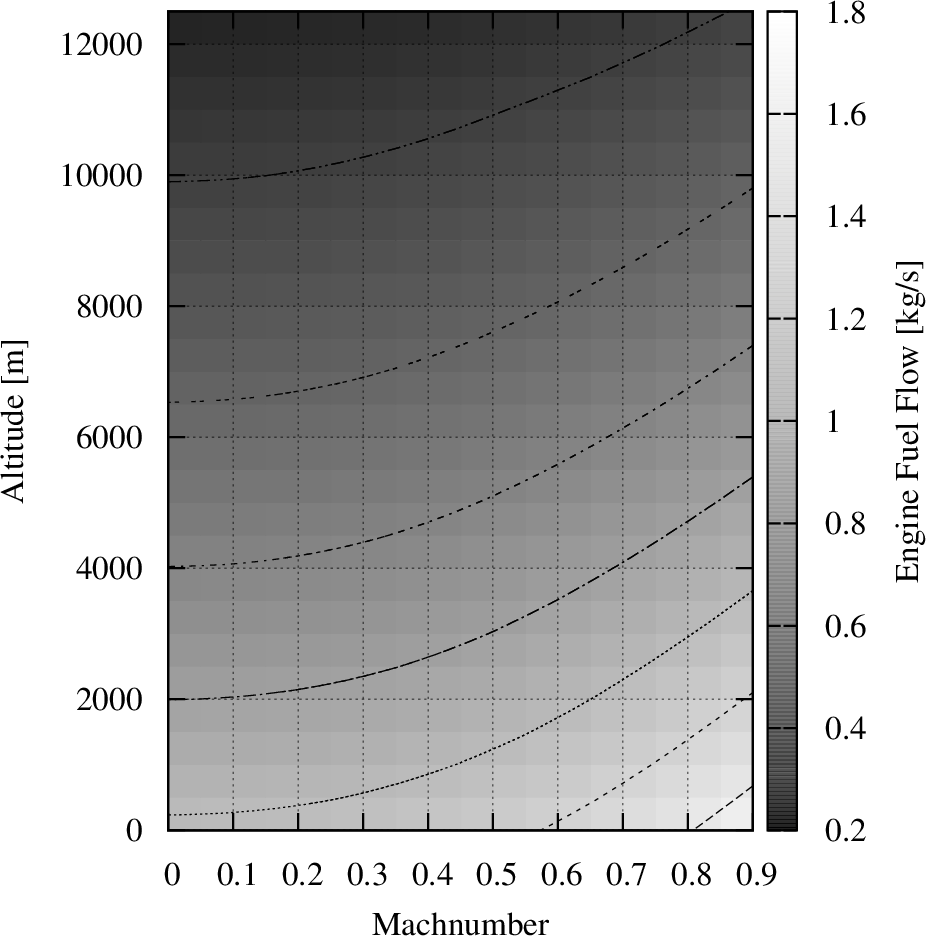
\includegraphics[keepaspectratio, width=\textwidth]{images/chap2/deck_ff.png}
		\caption{Fuel flow data.}
		\label{subfig:ceras_ff}	
	\end{subfigure}
	\caption{CERAS engine reference deck~\cite{bib:ceras}.}
	\label{fig:ceras_engine_deck}
\end{figure}

To this end, the ``rubber engine'' model has been developed by Roux in her Ph.D. thesis~\cite{bib:roux}: she based her equations on the previous formulations of Mattingly~\cite{bib:mattingly}, Jane Taylor~\cite{bib:janes}, Torenbeek~\cite{bib:torenbeek} and ESDU database~\cite{bib:esdu}. 
This model fixes the limitations of the CERAS deck, providing a set of equations to create the thrust and fuel flow maps, starting from a set of parameters: BPR, thrust at sea level, operating pressure ratio and temperature at the exit of the nozzle. 
It also provides the dimensions, giving an estimation of the engine wetted area, to consider also the impact on the aerodynamics.

\subsubsection{Geometry}
\label{subsubsec:chap2_fast_geom}

The geometry module is one of the key analyses to carry out, as it allows the definition of a viable aircraft, that satisfies OAD requirements, including balance and stability. 

Each aircraft component requires a set of input parameters from which it is possible to get geometrical properties and mass estimation. 
The choice of the entry parameters is not unique, but depends on the formulation; in FAST theoretical and statistical equations are applied, following the handbook provided by Airbus~\cite{bib:airbus_notes}.
Table~\ref{tab:fast_geom_entry_parameter} reports the set of parameters needed for each component; note that the wing needs the wing area, which is separately computed at step 2 of Fig.~\ref{fig:fast_basic}.  
Entries do not cover all the parameters needed: the remaining ones are computed starting from statistical equations that give the dependency with these entries.
As example, the thickness-to-chord ratio of the wing is computed considering the cruise Mach number, to take into account that it can not be too large to avoid compressibility at high speed~\cite{bib:airbus_notes}; in other formulations this parameter may be considered as input too. 
The same logic applied for the tails' aspect ratio and sweep. 
This aspect will become a key point in the development of the MDO problem, as it will be shown later.
\begin{table}[!h]
	\centering
	\begin{tabular}{c c c c}
		\hline
		\textbf{Fuselage} & \textbf{Wing} & \textbf{Tails} & \textbf{Engine and nacelle} \\
		\hline
		Number of passengers & Wing area & Taper ratio & Thrust at sea level \\
		Seats' dimensions & Aspect ratio & Thickness-to-chord ratio & Bypass ratio \\
		& Sweep angle & & \\
		& Taper ratio & & \\ 
		& Mach number & & \\
		\hline
	\end{tabular}
	\caption{Input parameters to properly size each geometrical component, according to the formulation used in FAST~\cite{bib:airbus_notes}.}
	\label{tab:fast_geom_entry_parameter}
\end{table}

The geometry analysis is an iterative procedure, that needs to converge, and thus it can be expressed with the usual xDSM diagram, as done in Fig.~\ref{fig:fast_geom_basic}. 
Corresponding algorithm is reported in Algorithm~\ref{alg:fast_geometry_basic}.
\begin{figure}[!h]
	\centering
	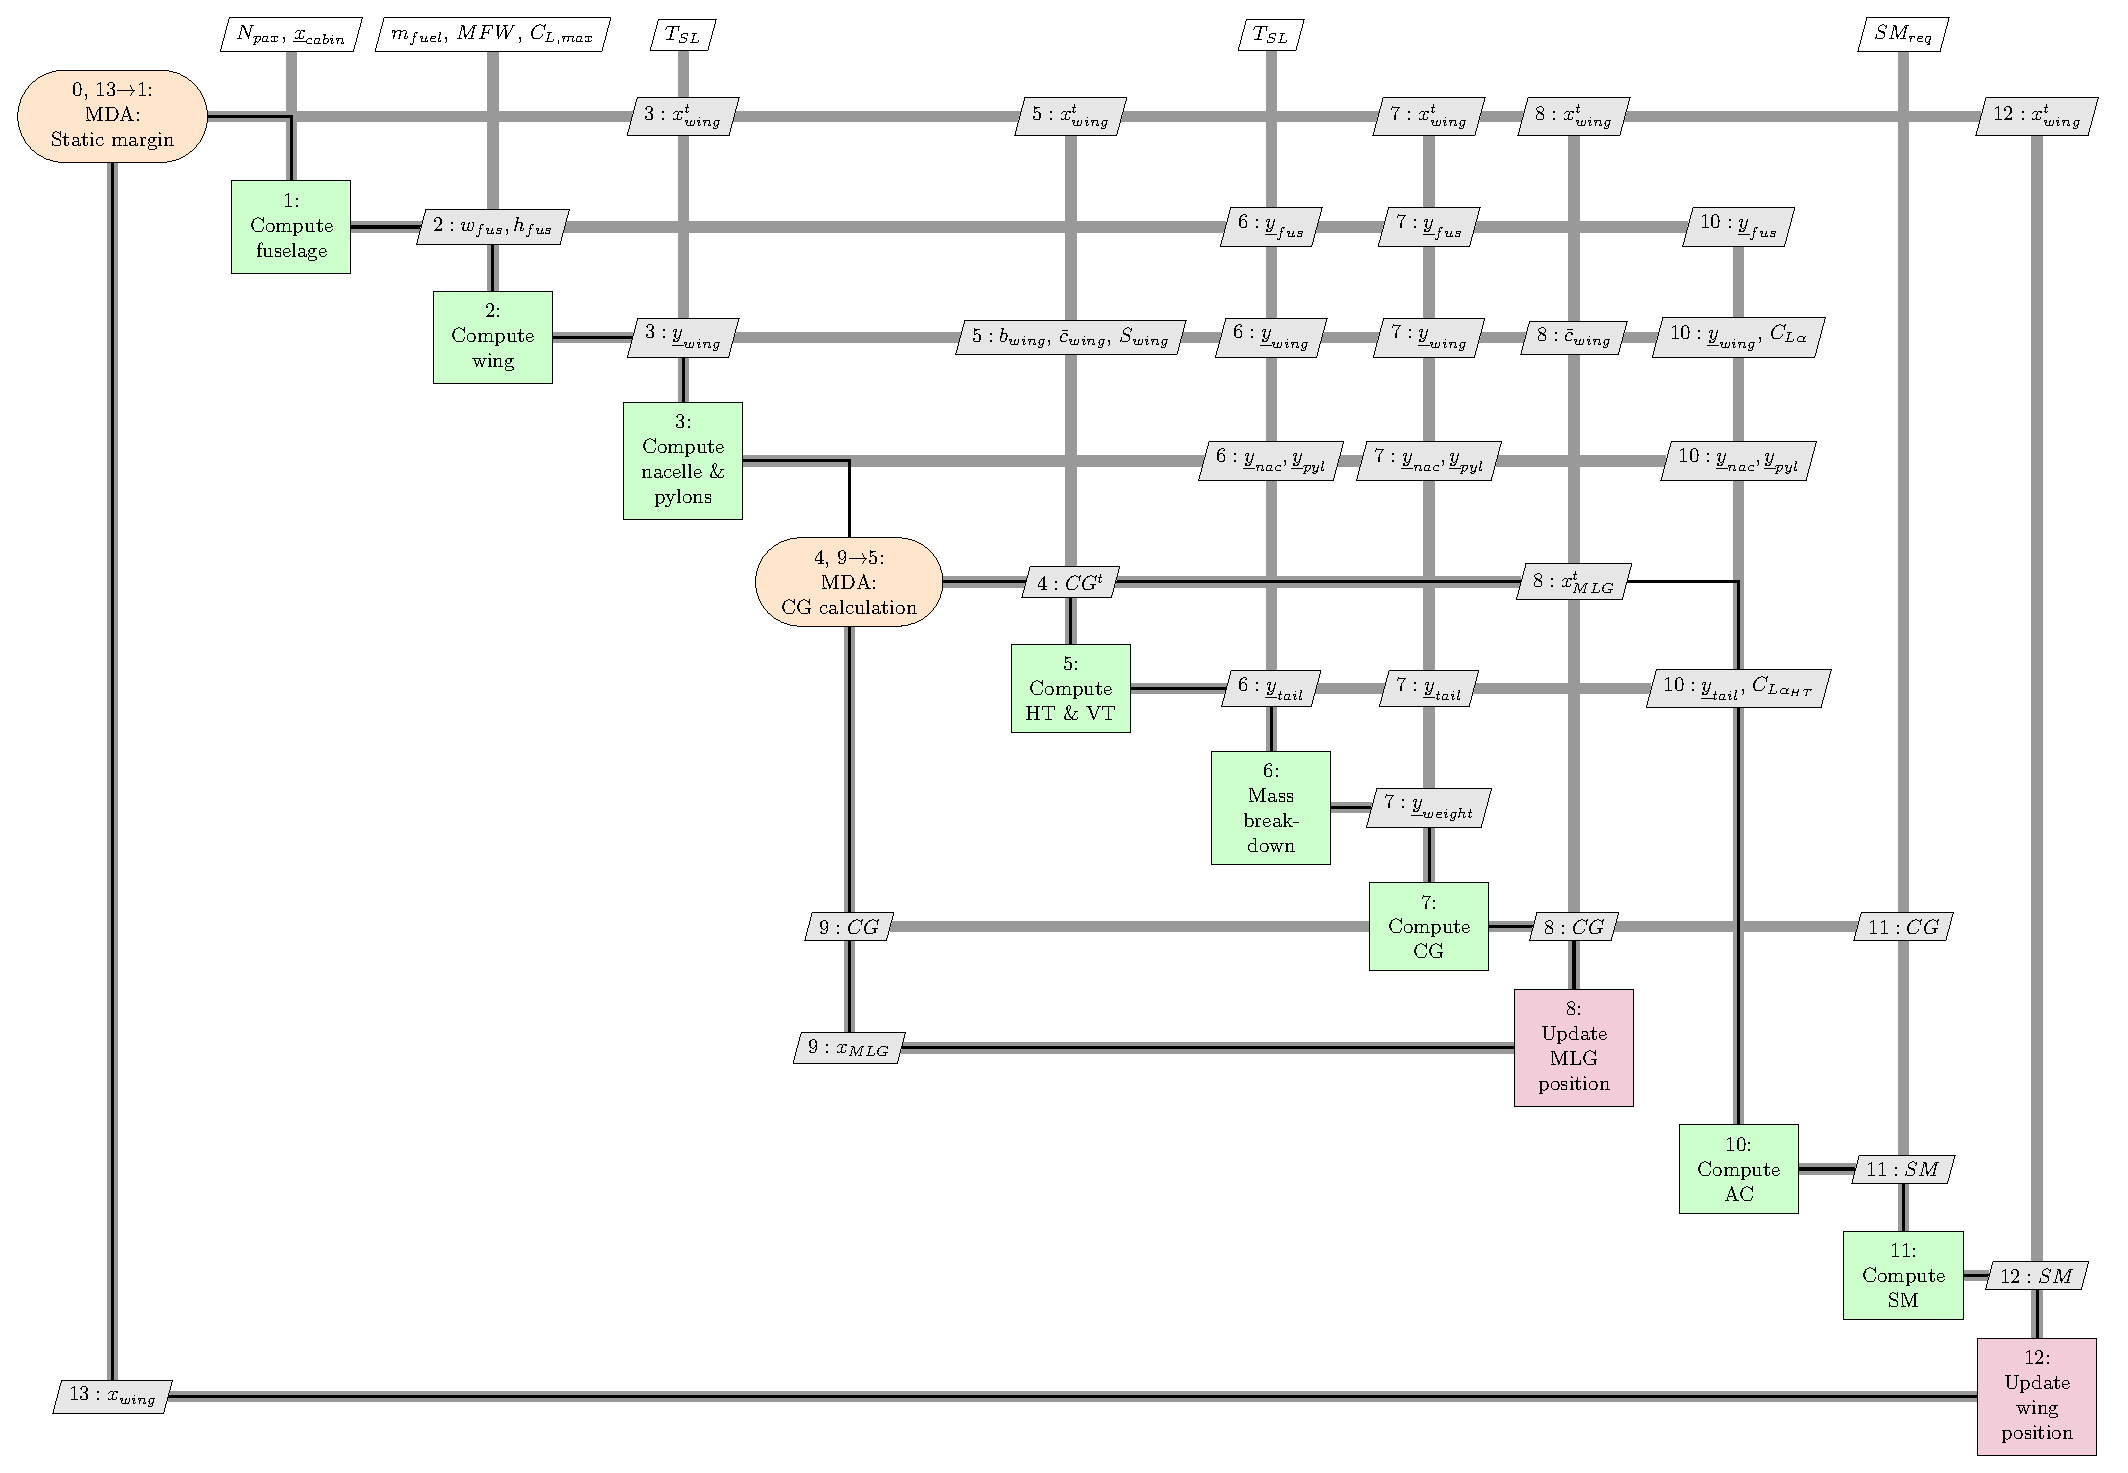
\includegraphics[keepaspectratio, width=1.2\textwidth, angle=90]{images/chap2/FAST_geometry}
	\caption{xDSM diagram of the geometry analysis coded in FAST~\cite{bib:lambe_xdsm}.}
	\label{fig:fast_geom_basic}
\end{figure}

\begin{algorithm}[!h]
	\caption{Algorithm for the geometry module of FAST, shown in Fig.~\ref{fig:fast_geom_basic}.}
	\label{alg:fast_geometry_basic}
	\begin{algorithmic}
		\REQUIRE Geometry design parameters.
		\ENSURE Aircraft geometry, that satisfied the required stability constraint.
		\STATE 0: Initialise the geometry resizing loop.
		\REPEAT
		\STATE 1: Compute the fuselage geometry, according to the required number of passengers and seat arrangement.
		\STATE 2: Compute the wing geometry, starting from the wing area information, deduced in a previous analysis.
		\STATE 3: Compute nacelles and pylons geometry.
		\STATE 4: Initialise the internal loop, to get the center of gravity.
		\REPEAT
		\STATE 5: Compute the empennages, horizontal and vertical tails, according to stability requirements.
		\STATE 6: Estimate the masses of all the components.
		\STATE 7: Estimation of the global center of gravity.
		\STATE 8: Update the main landing gear position, to get the global center of gravity.
		\UNTIL {$9 \rightarrow 5$: internal loop has converged.}
		\STATE 10: Estimate the aerodynamics center position.
		\STATE 11: Compute the static margin with Eq.~\eqref{eq:static_margin_def}.
		\STATE 12: Change the wing position, to match the static margin requirement.
		\UNTIL {$13 \rightarrow 1$ MDA has converged.} 
	\end{algorithmic}
\end{algorithm}

The diagram of Fig.~\ref{fig:fast_geom_basic} shows evidence of two iterative loops.
The outer loop is the main one, since it describes the full resizing process and it is driven by the stability requirement: the static margin SM must be included in an allowable range, given by certification. 
It is to revise that SM is defined as the distance between the center of gravity and aerodynamics center, normalized with respect to the mean aerodynamics chord: for stability it has to be negative~\cite{bib:anderson_perfo, bib:roskam_perfo}. 
However, FAST uses the opposite convention:
\begin{equation}
\label{eq:static_margin_def}
SM = \frac{x_{ac}-x_{cg}}{\bar{c}} 
\end{equation}
then for stability SM must be positive. 
Also, it can not be too high as value, otherwise the aircraft will be too stable to be easily controlled; the allowable domain, required by certification~\cite{bib:airbus_notes} is that SM is included between 5 and 10\%:
\begin{equation}
\label{eq:static_margin_limits}
0.05 \leq \textrm{SM} \leq 0.10
\end{equation}
Static margin depends mainly on the wing position: at each iteration, once that the geometry has converged, FAST controls the value of the SM and, if it exceeds the limits, it moves the wing to match the allowable range.
Then it proceeds to next iteration. 

The internal loop involves mainly the empennages and the landing gear.
At step 4 it initialises the values of horizontal and vertical tails, starting from volume coefficient estimation~\cite{bib:anderson_perfo}. 
Then it iteratively resizes the tails to ensure that the horizontal tail provides enough lift to balance the aircraft at the maximum center of gravity forward position (in the most penalizing conditions) and to respect condition given by Eq.~\eqref{eq:static_margin_limits}, and the vertical tail provides enough lateral force in cruise, to counterbalance the unstable yaw moment generated by the fuselage. 
These rules come from the work of Raymer~\cite{bib:raymer} and Kroo~\cite{bib:kroo_2001}.
At this point, the geometry module proceeds to the center of gravity estimation: in case it is out of the required range of variation, it updates the main landing gear position to fix it, to proceed at the next iteration, otherwise it proceeds with the SM estimation. 
The iterative loops give as output a viable geometry, starting from which the aerodynamics and the performances can be evaluated.

Finally, even if the wing area is computed outside this procedure, it is useful to spend some words on how it is calculated.
Its estimation is done at step 2 of Fig.~\ref{fig:fast_basic}, according to two requirements approach speed and fuel capacity. 
The first condition ensures that the wing area provides enough lift in approach, with flap and slat fully retracted, and can be represented by the lift equation as follow:
\begin{equation}
\label{eq:wing_approach_condition}
m_{L}g = \frac{1}{2}\rho V_{app}^2 S_{w_{app}} C_{L_{\max}}
\end{equation}
where $m_{L}$ is the maximum landing gear, $V_{app}$ the approach speed (23\% higher than the stall speed), $C_{L_{\max}}$ the maximum lift coefficient with flap and slat in landing configuration, and $S_{w_{app}}$ the minimum wing area needed to satisfy the equation. 

The second condition ensures that the wing is large enough to accomodate the fuel needed to complete the design mission. 
An estimation of wing capacity is provided by Raymer~\cite{bib:raymer}:
\begin{equation}
\label{eq:wing_fuel_condition}
m_{f_{\max}} = 224 S_{w_{f}}^{1.5}AR^{-0.4}\left[0.6\left(\frac{t}{c}\right)_{root}+0.4\left(\frac{t}{c}\right)_{tip}\right]+1570
\end{equation}
where $AR$ is the aspect ratio, $\frac{t}{c}$ is the thickness-to-chord ratio, evaluated at the wing root and tip, and $S_{w_{f}}$ the wing area. 
Imposing $m_{f_{\max}}=m_f$ yields to an estimation of the minimum wing area needed for the fuel storage.

The final wing area must respect both Eq.~\eqref{eq:wing_approach_condition} and Eq.~\eqref{eq:wing_fuel_condition}.
Thus the maximum value between the two estimations is chosen.
This procedure ensures a feasible value of wing area, however it is to note that it limits the exploration of the wing area to only two values, whereas the conditions described by Eq.~\eqref{eq:wing_approach_condition} and Eq.~\eqref{eq:wing_fuel_condition} may be written as inequalities, enlarging the values to explore that satisfy the conditions. 
As a conclusion, the estimated value may not be optimal, because of the limited design space, and FAST does not explore any other values but $S_{w_{app}}$ and $S_{w_{f}}$.

\subsubsection{Aerodynamics}
\label{subsubsec:chap2_fast_aero}

The aerodynamics module is devoted to the polar estimation $C_D=f\left(C_L\right)$, both for low and high speed. 
This analysis too is based on statistical and engineering equations~\cite{bib:airbus_notes}, enabling extremely fast computations
The drag coefficient is composed of three terms: friction drag $C_{D_{0}}$, induced drag $C_{D_{i}}$ and compressibility drag $C_{D_{c}}$.

Friction drag is the term due to the form, generally it does not depend by the flight condition and then is considered constant with the lift coefficient.
The formulation used in FAST depends solely on the wetted areas. 
First the friction coefficient is computed, with the Prandtl-Schlichting correlation~\cite{bib:monaghan}:
\begin{equation}
\label{eq:friction_coefficient}
c_f = \frac{0.455}{\left(1+0.126M^2\right)\left(\log_{10}Re\right)^{2.58}}
\end{equation}
where $M$ is the actual Mach number, $Re$ the Reynolds number. 
Then, the $C_{D_0}$ is computed as the sum of friction coefficients for each component:
\begin{equation}
\label{eq:cd0}
C_{D_{0}}=\sum_{i}c_{f_{i}}k_{f_{i}}\frac{S_{i_{wet}}}{S_w}
\end{equation}
where $c_{f_{i}}$ is the local friction coefficient, $S_{i_{wet}}$ the wetted surface of $i$-th component, and $k_{f_{i}}$ a corrective factor, to consider secondary aspects, such as the sweep effect. 
Note that the Reynolds number used in Eq.~\eqref{eq:friction_coefficient} is not constant, but varies for each component, since the reference length is different. 
The value of $C_{D_{0}}$ is corrected, to include a parasite drag effect, with a corrective factor depending on the total wetted area. 

The second term of the induced drag depends on the square lift coefficient, in agreement with Prandtl theory~\cite{bib:cdn_notes, bib:anderson_aero}, and it represents the greater contribution in the drag breakdown. 
It is computed as
\begin{equation}
\label{eq:cd_induced}
C_{D_{i}}= \frac{C_L^2}{\pi \left(AR\right) e}
\end{equation}
where $e$ is the Oswald factor, depending solely on the wing geometry and the Mach number, estimated using the method proposed by Ni\c{t}\u{a} and Scholz~\cite{bib:nita}. 

The induced drag is associated to the energy dissipated by the vortex at the wing trailing edge. 
These vortex generate a downwash, which must be taken into account in the drag calculation, and as well as in the needed deflection to trim the aircraft. 
This last effect generates a new source of drag, associated to trim, that is added to the induced drag and, at first istance, is computed as
\begin{equation}
\label{eq:cd_trim}
C_{D_{trim}}= 5.89\times 10^{-4} C_L
\end{equation}

Finally, the last term $C_{D_{c}}$ is associated to the presence of compressibility phenomena and shock wave on the wing. 
At low speed, it can be neglected, but in the transonic regime it is crucial to have a proper estimation of this term. 
Unfortunately, it is not an easy task to find a simple suited model, as it depends on multiple factors: Mach number, lift coefficient, wing geometry, but also flow properties. 
A good correlation is found in the Airbus notes, in which $C_{D_{c}}$ depends solely on the Mach number and $C_L$, as shown in Fig.~\ref{fig:cd_comp_example}, for a wing sweep of 28~\si{\deg} and a thickness-to-chord ratio of 12\%.
It must be noted that the tendencies vary from aircraft to aircraft; however, in the zone of interest for the flight of subsonic turbofan aircraft ($M=0.7-0.8$), the term is small and near zero, and thus the approximation works fine, despite the limitations. 
\begin{figure}[!h]
	\centering
	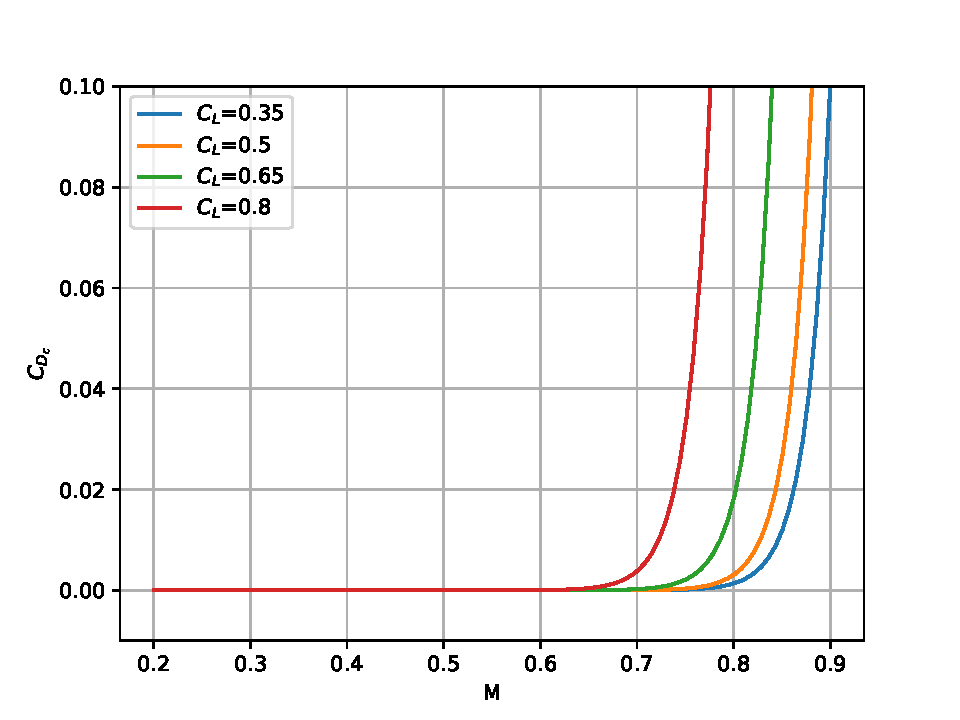
\includegraphics[keepaspectratio, width=0.7\textwidth]{images/chap2/cd_comp}
	\caption{Compressibility drag coefficient as function of Mach and lift coefficient. Curves are obtained considering $\Lambda_{25_{w}}$=28~\si{\deg} and $\left(\frac{t}{c}\right)_w$=0.12.}
	\label{fig:cd_comp_example}
\end{figure}

With all the terms are identified, the drag polar is computed as
\begin{equation}
\label{eq:cd_total}
C_D = k_{C_{D}}\left(k_{C_{D_{0}}}C_{D_{0}} + k_{C_{D_{i}}}C_{D_{i}} + k_{C_{D_{c}}} C_{D_{c}}\right)
\end{equation}
The $k$-terms are added to consider some improvements coming from the technologies, \textit{i.e.} the winglet design impact the induced drag, and this can be modeled using $k_{C_{D_{i}}}$. 

Alternatively to these equations, if desired, it is possible to use OpenVSP~\cite{bib:openvsp} for the calculations.
This code relies upon the VLM method, which is limited to incompressible flow, thus it is used only for low speed calculation, to get the slope $C_{L_{\alpha}}$ and the lift coefficient at zero angle of attack $C_{L_{0}}$. 
In real, VLM is limited to inviscid flow too, but OpenVSP offers a correction based on wetted areas.
FAST interfaces also with XFoil~\cite{bib:xfoil} for the airfoil aerodynamics, mainly used in the estimation of the maximum $C_L$ at low speed. 
To account for the three-dimensionality introduced by the sweep, the cosinus law is considered~\cite{bib:abbott, bib:cdn_notes, bib:anderson_aero}:
\begin{equation}
\label{eq:cl_max_3d}
C_{L_{\max}} = k_{w}C_{l_{\max}}\cos\Lambda_{25_{w}}
\end{equation}

\subsubsection{Mass estimation}
\label{subsubsec:chap2_fast_mass}

The mass breakdown used in FAST follows the French standard 2001/B~\cite{bib:mass_breakdown}, which is reported in Table~\ref{tab:mass_breakdown_standard} for sake of clarity. 
The OWE is divided into five parts: airframe, propulsion, systems, operational items and crew.
Adding payload and fuel, the MTOW is obtained. 
\begin{table}[!h]
	\centering
	\begin{tabular}{l l}
		\hline
		\textbf{A} & \textbf{Airframe} \\
		A1 & Wing \\
		A2 & Fuselage \\
		A3 & Horizontal and Vertical tail \\
		A4 & Flight controls \\
		A5 & Landing gear \\
		A6 & Pylons \\
		A7 & Paint \\
		\textbf{B} & \textbf{Propulsion} \\
		B1 & Engines \\
		B2 & Fuel and oil systems \\
		B3 & Unusable oil and fuel \\
		\textbf{C} & \textbf{Systems and fixed installations} \\
		C1 & Power systems (APU, electrical and hydraulical system) \\
		C2 & Life support systems (Pressurization, de-icing, seats, ...) \\
		C3 & Instrument and navigation \\
		C4 & Transmissions \\
		C5 & Fixed operational systems (radar, cargo hold mechanization) \\
		C6 & Flight kit \\
		\textbf{D} & \textbf{Operational items} \\
		D1 & Cargo equiment \\
		D2 & Passenger seats \\
		D3 & Catering equipment \\
		D4 & Passenger safety equipment \\
		D5 & Cabin toilet equipment \\
		\textbf{E} & \textbf{Crew} \\
		\textbf{F} & \textbf{Fuel} \\
		\textbf{G} & \textbf{Payload} \\		
		\hline
	\end{tabular}
	\caption{Mass breakdown standard, according to the French norm 2001/B~\cite{bib:mass_breakdown} and implemented in FAST.}
	\label{tab:mass_breakdown_standard}
\end{table} 

For parts B, C, D, and E statistical equations, reliable for standard TAW configugrations, are used.
The airframe part is the most complicated, since in general the components need to satisfy different critical conditions, according to certification. 
As example, the wing is sized to carry out the aerodynamics load, but also to limit the torsion and the bending moment and avoid aeroelasticity issues; fuselage instead needs to carry on the pressurization load, and pass the stress analyses~\cite{bib:megson}. 
Generally, for these parts, FEM or even experimental tests are used; thanks to the experience gained throughout the years, surrogate models have been developed: they are accurate as far as the configuration does not change from the TAW. 
These models, collected in the Airbus note~\cite{bib:airbus_notes}, are implemented in FAST. 

To consider the impact of different technologies, notoriously the use of new materials like composite or advanced alluminium alloy, the same technique based on the corrective factors $k$ is used: each element listed in Table~\ref{tab:mass_breakdown_standard} has its own $k$-factor, to model a reduction or increase in mass (in percentage), as proposed by Kirby~\cite{bib:kirby}.

\subsubsection{Performance}
\label{subsubsec:chap2_fast_perfo}

The performance analysis is based on the point mass approach: the aircraft is represented as a mass point, and the mission over the time is computed through a time step integration. 
For each time step, the code carries out the following analyses:
\begin{enumerate}
	\item First, the actual atmospheric data, starting from the actual altitude, are computed using the ISO standard atmosphere.
	
	\item Then, using the lift equation FAST computes the actual value of $C_L$:
	\begin{equation}
	\label{eq:lift_equation}
	C_L = \frac{mg}{\frac{1}{2}\rho V^2 S_w}.
	\end{equation}
	The drag coefficient $C_D$ is obtained interpolating the polar data with the actual value of $C_L$.
	
	\item As third step, performance analysis computes the actual propulsive data. 
	In case of balanced longitudinal flight (that is, during the cruise leg), the thrust required is already known imposing that the aircraft has no climb angle: 
	\begin{equation}
	\label{eq:balanced_flight}
	\left\{\begin{array}{l}
	L = mg \\
	D = T
	\end{array}\right.
	\end{equation} 
	In case of non balanced flight (that is, when the aircraft is climbing or descending), the thrust is obtained interpolating the engine deck on a given thrust rate, and the climb angle is computed solving the non balanced longitudinal flight equations:
	\begin{equation}	
	\label{eq:non_balanced_flight}
	\left\{\begin{array}{l}
	L\cos\gamma = mg \\
	D = T + L\sin\gamma	
	\end{array}\right.	
	\end{equation}
	In both cases, the SFC is calculated, to consider the mass variation.
	
	\item Finally, FAST updates the state vector recomputing the new value of velocity and mass
	\begin{equation}
	\label{eq:mass_perfo_update}
	m_{i+1} =  m_i - \textrm{T}(\textrm{SFC})\Delta t
	\end{equation}
	and proceeds to next iteration, using the new state vector as initial point of the following time step.
\end{enumerate}

This process can be schematised using an xDSM diagram, as shown in Fig.~\ref{fig:fast_mission_segment}.
\begin{figure}[!h]
	\centering
	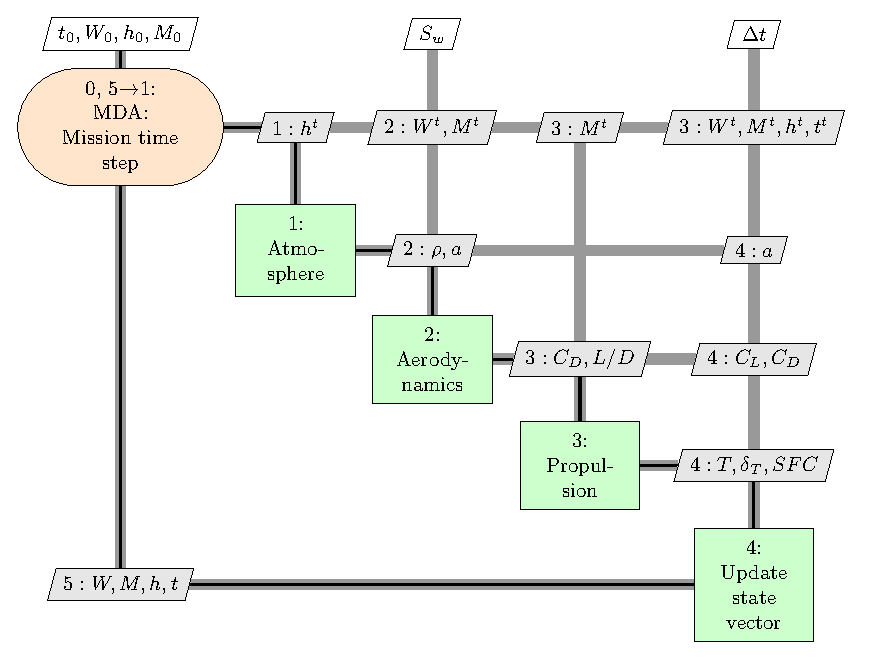
\includegraphics[keepaspectratio, width=0.6\textwidth]{images/chap2/FAST_mission_segment}
	\caption{xDSM diagram for the time step performance analysis.}
	\label{fig:fast_mission_segment}
\end{figure}

This routine allows to get a detailed trajectory. 
The mission is made up by takeoff, initial climb up to 1500~ft, climb to reach the cruise altitude, cruise, descent, an alternate flight plus holding phase to consider reserve calculation, and finally landing. The cruise altitude is found imposing that the initial point corresponds to the maximum lift-to-drag ratio; then it is possible to choose between two cruise phases: a conventional step climb and a cruise climb approach. 
They are shown in Fig.~\ref{fig:mission_profile}.
\begin{figure}[!h]
	\centering
	\begin{subfigure}{0.8\textwidth}
		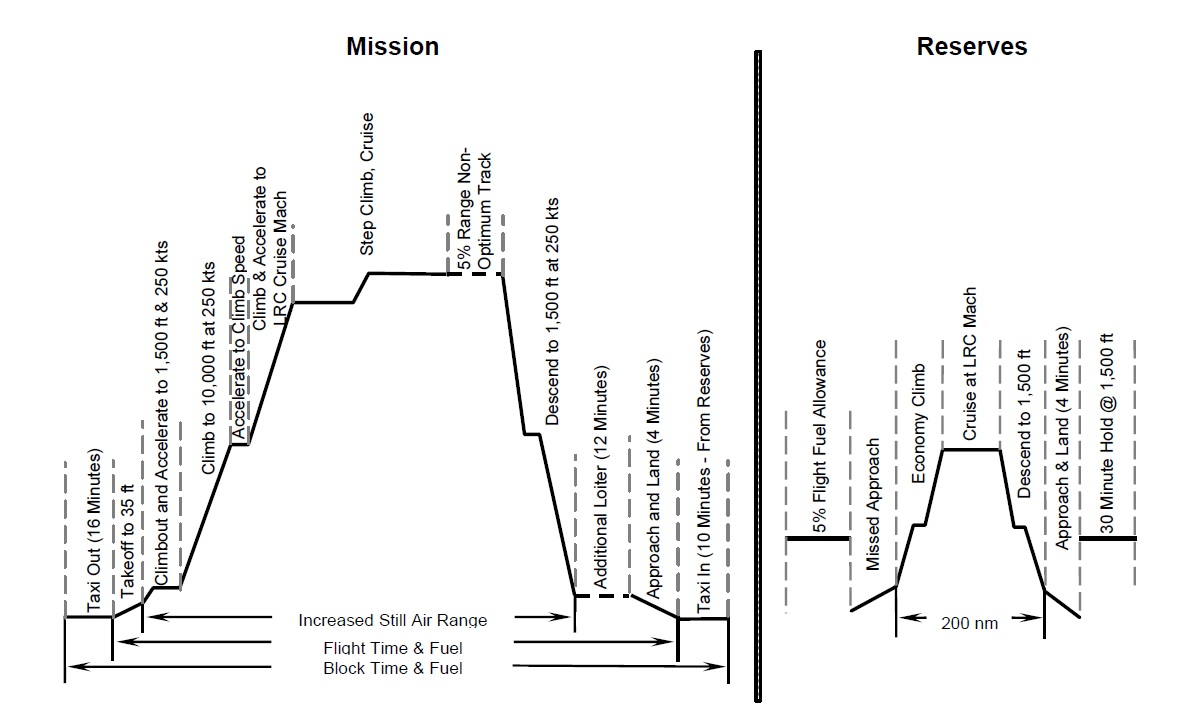
\includegraphics[keepaspectratio, width=\textwidth]{images/chap2/step_climb.jpg}
		\caption{Step climb mission.}
		\label{subfig:step_climb}
	\end{subfigure}
	\begin{subfigure}{0.8\textwidth}
		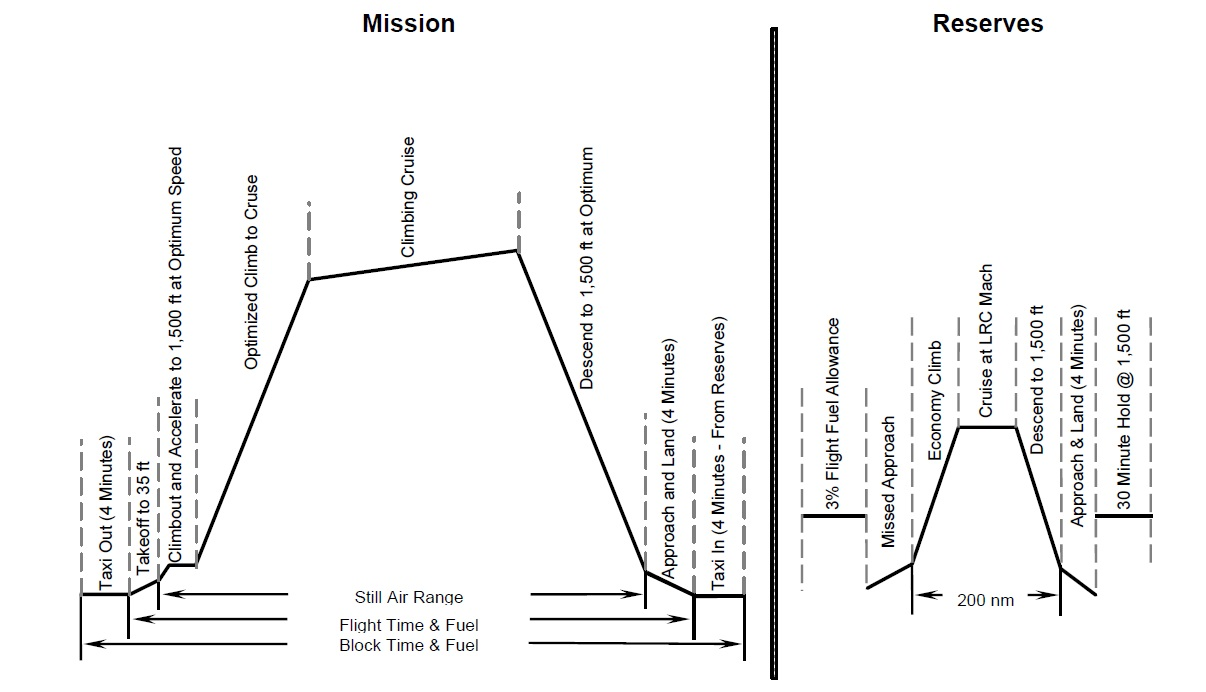
\includegraphics[keepaspectratio, width=\textwidth]{images/chap2/cruise_climb.jpg}
		\caption{Cruise climb mission.}
		\label{subfig:cruise_climb}
	\end{subfigure}
	\caption{Different mission profiles~\cite{bib:bradley_sugar_p1}.}
	\label{fig:mission_profile}
\end{figure}

The step climb approach recalls the real aircraft trajectory, for which it is mandatory to fly on predefined flight level according to the air traffic management rules~\cite{bib:mission_path_def}. 
The step climb is done only if it advantageous for fuel saving, otherwise the aircraft continues on the same level. 
However, according to NASA perspectives~\cite{bib:bradley_sugar_p1}, the cruise climb option will replace the step climb, since it requires that the aircraft always flies at its maximum lift-to-drag ratio, saving fuel. 
This new mission is also included as one of the most innovative aspects in the new air traffic management rules for a more sustainable aviation~\cite{bib:bradley_sugar_p1}.
From a coding point to view, the cruise climb approach is less time consuming than the step cruise, since at each iteration the code does not need to check if it is advantageous to perform a climb of 2000~ft.

When in the cruise leg, the descent function is called at each time step, to know the total distance travelled: in case this value is below the range, it proceeds to a new time step. 
This algorithm is not efficient, as the descent function is called many times (about 1000). 
This point is identified as an area of improvement for FAST. 
The procedure is also shown in Fig.~\ref{fig:fast_performance_basic} and described in Algorithm~\ref{alg:fast_performance_basic}, to better highlight the point. 
For clarity, only the two iterative loops, to find the cruise altitude and to cover the range, are shown; a complete diagram must include ground operation before the climb and reserve calculation after the descent. 
\begin{figure}[!h]
	\centering
	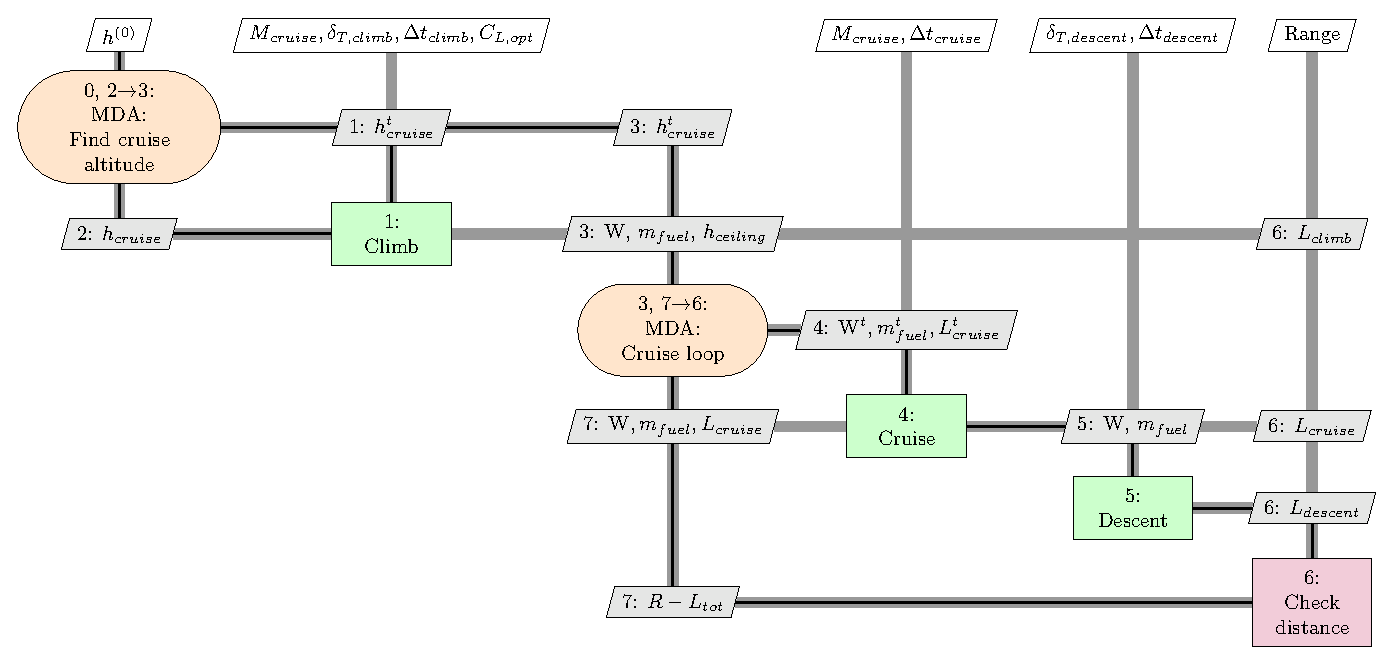
\includegraphics[keepaspectratio, width=\textwidth]{images/chap2/FAST_performance}
	\caption{xDSM diagram climb and cruise phase performance, to highlight the iterative procedure used in FAST.}
	\label{fig:fast_performance_basic}
\end{figure}

\begin{algorithm}[!h]
	\caption{Algorithm for climb and cruise phase performance, with reference to xDSM diagram shown in Fig.~\ref{fig:fast_performance_basic}.}
	\label{alg:fast_performance_basic}
	\begin{algorithmic}
		\REQUIRE MTOW and polar.
		\ENSURE Detailed trajectory calculation.
		\STATE 0: Initialise the climb loop.
		\REPEAT
		\STATE 1: Compute the climb and check if the final altitude corresponds to the maximum lift-to-drag ratio.
		\STATE 2: If the final climb altitude does not correspond to that of maximum lift-to-drag ratio, compute a new value, otherwise proceed to next iteration.
		\UNTIL {$2 \rightarrow 1$: initial cruise altitude is found.}
		\REPEAT
		\STATE 3: Initialise the state vector for the cruise phase.
		\STATE 4: Perform a time step of cruise leg.
		\STATE 5: Compute the descent leg.
		\STATE 6: Compute the difference between the required range and the total distance travelled.
		\STATE 7: Check if the difference of step 6 is equal to zero: if not, proceed to a new time step.
		\UNTIL {$7 \rightarrow 1$ total required range is covered.} 
	\end{algorithmic}
\end{algorithm}

\subsubsection{CCM -- Certification Constraint Module}
\label{subsubsec:chap2_ccm}

The Certification Constraints Module, abbreviated as CCM by now, is the module developed by Schmollgruber during his Ph.D.~\cite{bib:schmollgruber, bib:schmollgruber_phd}. 
The scope of the CCM is to check if certification specifications are respected: indeed, it is not sufficient that the aircraft is viable, but it must comply with the EASA/FAA rules.

The module works outside the sizing loop: it limits to control if the aircraft complies with certifications, but in case one of the rules is not satisfied, it does not proceed by itself to any correction. 
It is up to the user to go back manually and change the design parameter to get the certifications satisfied.
However, it may be integrated within an optimisation loop, where the conditions are design constraints, and the algorithm may find the optimum design that satisfies all the rules above. 
This procedure has been set by Schmollgruber, who used \texttt{Scipy} libraries to carry out an optimisation based on certifications~\cite{bib:schmollgruber_phd}.

The CCM module relies upon a \texttt{xml} file, which contains the prescribed conditions to check, using the meta-model GAMME as for the I/O file~\cite{bib:bedouet}.
The documents considered are the CATPOL~\cite{bib:catpol} and CS-25~\cite{bib:cs25}, that are related to large passenger aircraft and prescribe the conditions to be respected en-route and during takeoff and landing (the most stringent segments), with all engines operative and in case of failure. 
For each case, the CCM solves the flight equations using the Python function \texttt{fsolve}.
The details of rules are listed below; for shortness the acronym AEO is used to indicate the condition of all engine operative, and OEI to indicate the one engine inoperative condition. 
\begin{itemize}
	\item \textbf{CAT.POL.A.410(a)}. This paragraph of the CATPOL document~\cite{bib:catpol} prescribes that, in en-route condition with all the engines operative, at the top of climb (1) and top of descent (2) the aircraft must preserve a reserve of vertical speed not below than 300~ft/min.
	
	\item \textbf{CS-25.119(a)}. This rule, from CS-25 specifications for large passenger aircraft~\cite{bib:cs25}, requires that in landing condition with AEO, the steady gradient flight must not be less than 3.2\%.
	
	\item \textbf{CS-25.121(a)}. This rule requires that, during takeoff with landing gear extracted and OEI condition, the steady gradient flight must be positive. 
	
	\item \textbf{CS-25.121(b)}. This rule requires that, during takeoff and OEI condition, at the point of flight path when the landing gears are fully retracted (400~ft), the steady gradient flight must not be less than 2.4\%.
	
	\item \textbf{CS-25.121(c)}. This rule requires that, in en-route configuration at the end of takeoff and in OEI condition, the steady gradient flight must not be less than 1.2\%.
	
	\item \textbf{CS-25.121(d)}. This rule requires that, in approach configuration with AEO condition, the steady gradient flight must not be less than 2.1\%.
\end{itemize} 

Table~\ref{tab:ccm_rules} sums up the rules, together with the flight path specified and the minimum value of parameters required. The notation $V_{z}$ indicates the vertical speed, meanwhile $\gamma_{\%}$ the steady gradient flight in percentace.
\begin{table}[!h]
	\centering
	\begin{tabular}{l c c c c}
		\hline
		\textbf{Certification} & \textbf{Phase} & \textbf{Condition} & \textbf{Parameter} & \textbf{Min. value} \\
		\hline
		CAT.POL.A.410(a)-1 & Top of climb & AEO & $V_{z}$ & 300~ft/min \\
		CAT.POL.A.410(a)-2 & Top of descent & AEO & $V_{z}$ & 300~ft/min \\
		CS-25.119(a) & Landing & AEO & $\gamma_{\%}$ & 3.2~\% \\
		CS-25.121(a) & Takeoff & OEI & $\gamma_{\%}$ & 0~\% \\
		CS-25.121(b) & 400~ft & OEI & $\gamma_{\%}$ & 2.4~\% \\
		CS-25.121(c) & End of takeoff & OEI & $\gamma_{\%}$ & 1.2~\% \\
		CS-25.121(d) & Approach & AEO & $\gamma_{\%}$ & 2.1~\% \\
		\hline
	\end{tabular}
	\caption{CATPOL~\cite{bib:catpol} and CS-25~\cite{bib:cs25} rules explanation, considered in the CCM module of FAST. $V_{z}$ represents vertical speed, meanwhile $\gamma_{\%}$ the gradient flight.}
	\label{tab:ccm_rules}
\end{table}

\subsection{Test case: Airbus A320}
\label{subsec:chap2_fast_test_case}

FAST has been developed for designing large passenger aircraft, using turbofan as engine. 
The validation case, presented by Schmollgruber et al.~\cite{bib:fast_main}, is the Airbus A320~\cite{bib:a320_specifications}, with the top level requirements reported in Table~\ref{tab:fast_base_tlar}.
The geometrical inputs required are instead reported in Table~\ref{tab:fast_base_geom_inp}, following the list presented in Table~\ref{tab:fast_geom_entry_parameter}.
Finally, Table~\ref{tab:fast_base_thrust_rate_entry} reports the thrust rate for each mission segment. 
\begin{table}[!h]
	\centering
	\begin{tabular}{l r r}
		\hline
		Range & 2750 & nmi \\
		Number of passengers & 150 & \\
		Approach speed & 132 & \si{\knot} \\
		Design payload & 13608 & \si{\kilogram} \\
		\hline		
	\end{tabular}
	\caption{Top level requirements for the A320 CERAS validation case used in FAST.}
	\label{tab:fast_base_tlar}
\end{table}
\begin{table}[!h]
	\centering
	\begin{tabular}{l r l}
		\hline
		$AR_w$ & 9.5 & \\
		$\Lambda_{25_{w}}$ & 25 & \si{\deg} \\
		$\lambda_w$ & 0.38 & \\
		$\lambda_{HT}$ & 0.4 & \\
		$\left(\frac{t}{c}\right)$ & 0.1 & \\
		$\lambda_{VT}$ & 0.3 & \\
		$\left(\frac{t}{c}\right)$ & 0.13 & \\
		\hline
	\end{tabular}
	\caption{Geometrical inputs for the A320 CERAS validation case.}
	\label{tab:fast_base_geom_inp}
\end{table}
\begin{table}[!h]
	\centering
	\begin{tabular}{l c}
		\hline
		Segment & $\delta_T$ \\
		\hline
		Taxi & 0.3 \\
		Takeoff & 1.0 \\
		Climb & 0.93 \\
		Cruise & Computed \\
		Descent & 0.55 \\
		Alternate climb & 0.93 \\
		Alternate cruise & Computed \\
		Alternate descent & 0.55 \\
		Hold & Computed \\
		Landing & 0.03 \\
		\hline
	\end{tabular}
	\caption{Thrust rate definition for each mission segment for the A320 CERAS validation case.}
	\label{tab:fast_base_thrust_rate_entry}
\end{table}
Actually, even if the Airbus A320 specification manual contains many geometrical information, as well as cargo disposition, it does not have any information regarding the mass breakdown, performance and the engine map. 
Thus, in FAST, the CERAS data are considered for comparison~\cite{bib:ceras}, since it emulates the Airbus A320 aircraft; engine model is direcly taken from the website. 
All the performances of this reference aircraft are available, and thus are used for the comparison. 

The results of FAST, for the A320, are shown in Fig.~\ref{fig:fast_base_results}: the climb and descent profile are depicted in Fig.~\ref{fig:fast_base_climb} and Fig.~\ref{fig:fast_base_descent}, meanwhile the global profile, using both the step cruise and the cruise climb, are shown in Fig.~\ref{fig:fast_base_cruise_step} and Fig.~\ref{fig:fast_base_cruise_climb}. 
The drag polar is reported in Fig.~\ref{fig:fast_base_polar}, while the payload range diagram of Fig.~\ref{fig:fast_base_pl_range} ends the set of output available. 
Note that the mission profile is very detailed and mimics a real aircraft trajectory, according to the air traffic rules~\cite{bib:mission_path_def}.
\begin{figure}[!h]
	\centering
	\begin{subfigure}{0.45\textwidth}
		\centering
		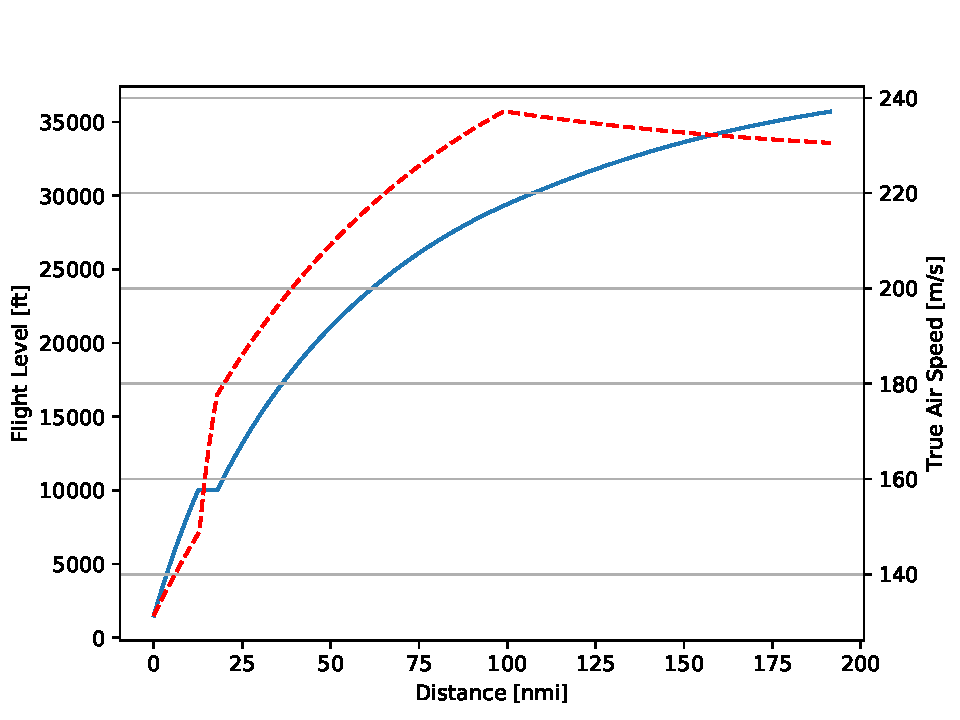
\includegraphics[keepaspectratio, width=\linewidth]{images/chap2/FAST_base_climb_profile}
		\caption{Climb profile.}
		\label{fig:fast_base_climb}
	\end{subfigure}
	\hspace{10mm}
	\begin{subfigure}{0.45\textwidth}
		\centering
		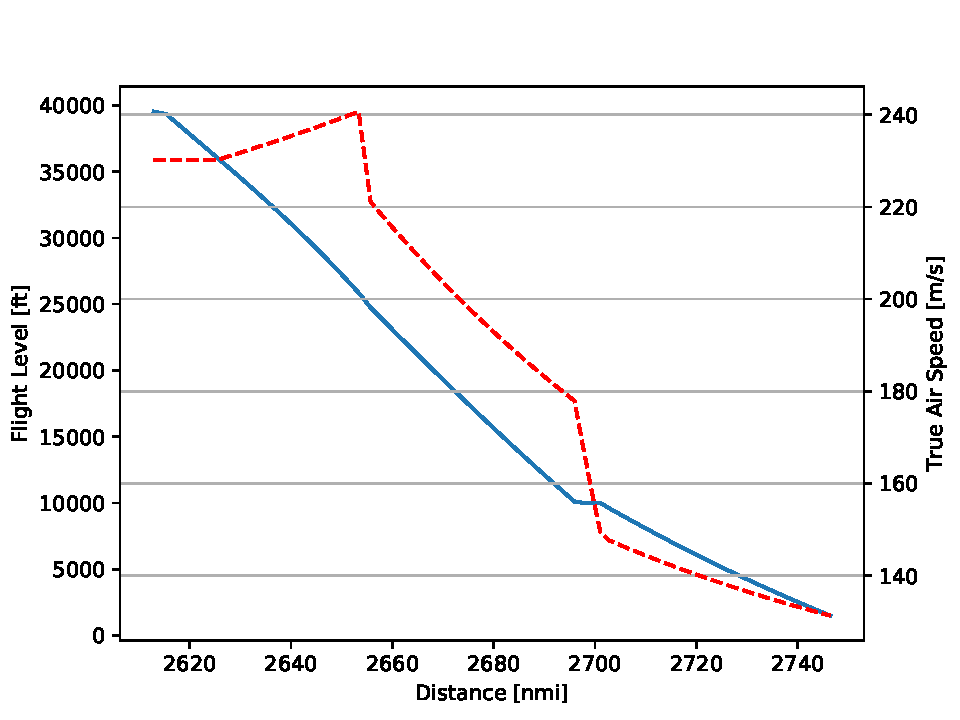
\includegraphics[keepaspectratio, width=\linewidth]{images/chap2/FAST_base_descent_profile}
		\caption{Descent profile.}
		\label{fig:fast_base_descent}
	\end{subfigure}
	
	\begin{subfigure}{0.45\textwidth}
		\centering
		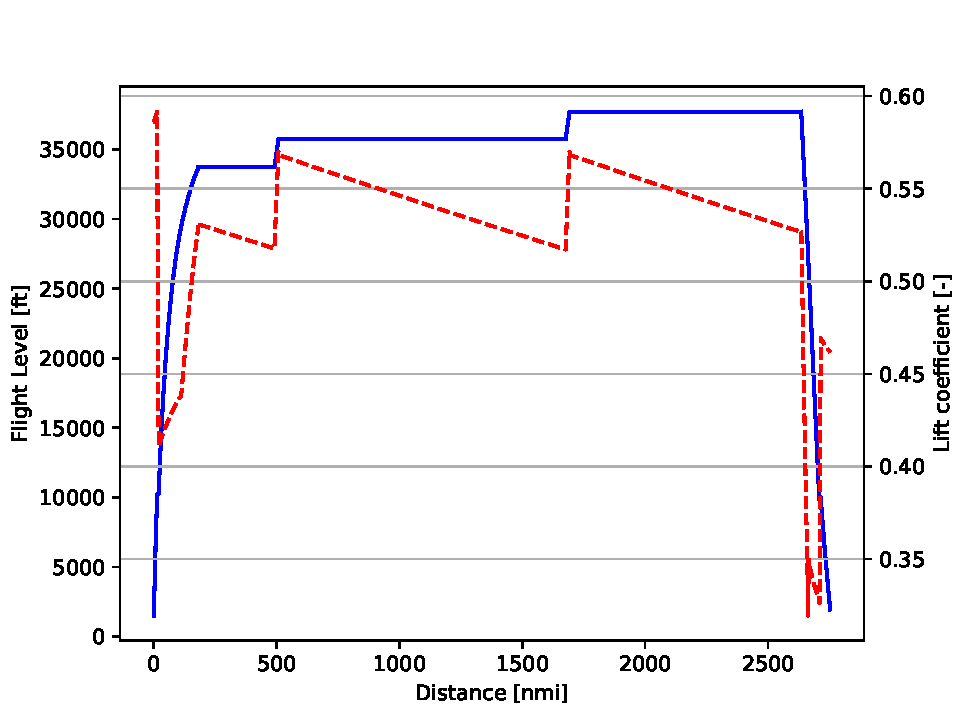
\includegraphics[keepaspectratio, width=\linewidth]{images/chap2/FAST_base_cruise_step_profile}
		\caption{Step cruise profile.}
		\label{fig:fast_base_cruise_step}
	\end{subfigure}	
	\hspace{10mm}
	\begin{subfigure}{0.45\textwidth}
		\centering
		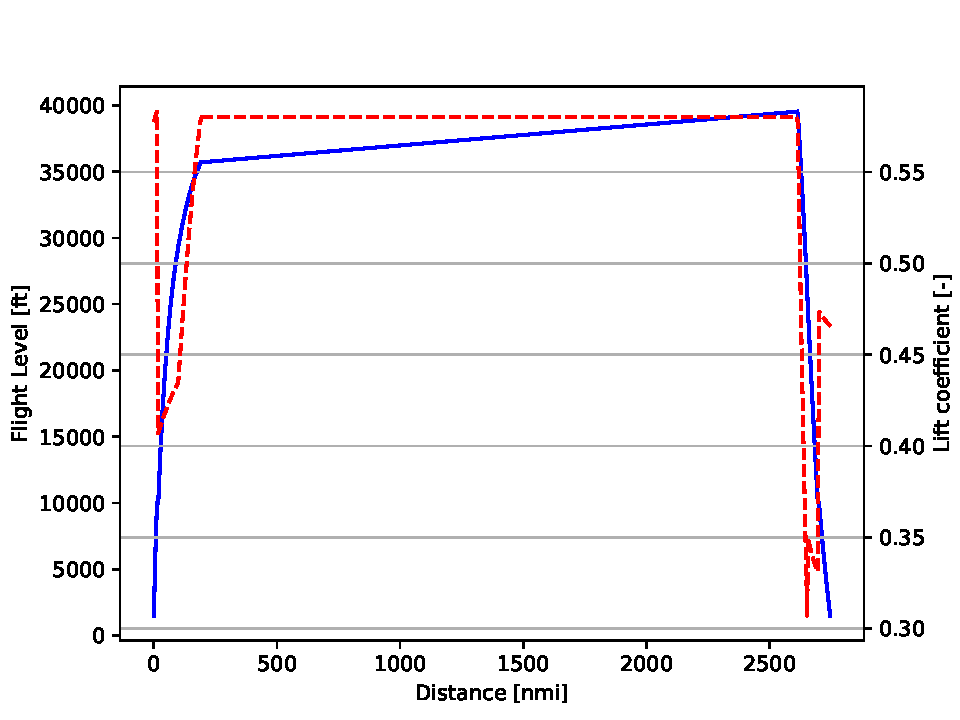
\includegraphics[keepaspectratio, width=\linewidth]{images/chap2/FAST_base_cruise_climb_profile}
		\caption{Cruise climb profile.}
		\label{fig:fast_base_cruise_climb}
	\end{subfigure}
	
	\begin{subfigure}{0.45\textwidth}
		\centering
		\includegraphics[keepaspectratio, width=\linewidth]{images/chap2/FAST_base_polar}
		\caption{Drag polar.}
		\label{fig:fast_base_polar}
	\end{subfigure}
	\hspace{10mm}
	\begin{subfigure}{0.45\textwidth}
		\centering
		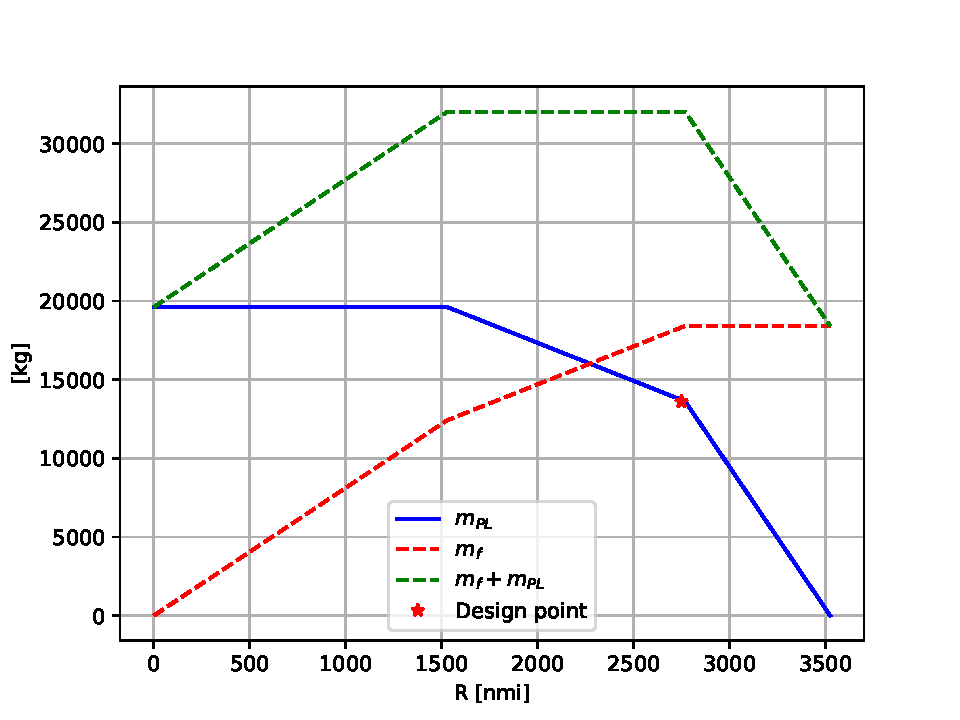
\includegraphics[keepaspectratio, width=\linewidth]{images/chap2/FAST_base_pl_range}
		\caption{Payload-Range diagram.}
		\label{fig:fast_base_pl_range}
	\end{subfigure}
	\caption{Some of the outputs of FAST, related to the A320 validation test case, with the TLAR reported in Table.~\ref{tab:fast_base_tlar}.
	Continuous line represents the trajectory, meanwhile dashed line is the true air speed or the lift coefficient, according to the flight phase.}
	\label{fig:fast_base_results}
\end{figure}

Table~\ref{tab:fast_base_comparison} reports the comparison between FAST, using both the step climb and the cruise climb approach, and the reference aircraft: it can be seen that the results are consistent, since the maximum difference is always less than 1\%. 
It must be highlighted that the step cruise and the cruise climb results are similar, but the computational cost of the second approach is reduced, because it does not need to check if it is convenient or not to perform a step of 2000~ft. 
For this reason, only this approach will be used for the future simulations. 
\begin{table}[!h]
	\centering
	\begin{tabular}{l l c c c}
		\hline
		& & \textbf{Step climb} & \textbf{Cruise climb} & \textbf{A320 CERAS} \\
		\hline
		MTOW & [\si{\kilogram}] & 74168.96 & 74562.82 & 74102.34 \\
		OWE & [\si{\kilogram}] & 42200.58 & 42190.71 & 42120.22 \\
		Wing area & [\si{\square\meter}] & 122.74 & 122.68 & 122.41 \\
		Mission fuel & [\si{\kilogram}] & 18799.11 & 18798.85 & 18678.12 \\
		\hline
	\end{tabular}
	\caption{Comparison between the results obtained in FAST and the A320 CERAS data~\cite{bib:fast_main}.}
	\label{tab:fast_base_comparison}
\end{table}

The CCM results are instead presented in Table~\ref{tab:fast_base_ccm}: the aircraft is compliant with both CATPOL and CS-25 specifications, with a safe margin for all the parameters.
The margin is taken to consider the case of hot day, with airport at high altitude (for the Airbus A320, La Paz airport is considered, which is 2000~\si{\meter} above the sea level).
\begin{table}[!h]
	\centering
	\begin{tabular}{l r l}
		\hline
		\textbf{CAT.POL.A.410(a)-1} & 964.69 & ft/min \\
		\textbf{CAT.POL.A.410(a)-2} & 1031.82 & ft/min \\
		\textbf{CS-25.119(a)} & 19.46 & \% \\
		\textbf{CS-25.121(a)} & 1.61 & \% \\
		\textbf{CS-25.121(b)} & 3.43 & \% \\
		\textbf{CS-25.121(c)} & 5.56 & \% \\
		\textbf{CS-25.121(d)} & 7.19 & \% \\
		\hline
	\end{tabular}
	\caption{CCM results for the A320 CERAS validation case.}
	\label{tab:fast_base_ccm}
\end{table}

Finally, some remarks on the computational time: the idea at the basis of FAST is to have a reliable code capable to deal with multidisciplinarity of aircraft design process and to have a result in a short time. 
The complete sizing process is done in 15-30 minutes, with the variation being associated with various TLAR and CPU performance level.
For the specific case of the reference Airbus A320 aircraft, the code runs for 25 minutes using the step climb approach and 20 minutes using the cruise climb approach. 
Preliminary tests indicated that the recoding of the cruise segment, as stated in Sec.~\ref{subsubsec:chap2_fast_perfo}, could lead to a reduction of CPU time of 5 to 10 minutes.

\section{OpenMDAO -- a multidisciplinary optimisation platform}
\label{sec:chap2_openmdao_overview}

OpenMDAO has ben created because of the need of NASA to have its own MDAO framework, in 2012, when v1.0 was released~\cite{bib:gray_omdao_2012, bib:gray_omdao_2014}. 
The code has been continuously developed throughout the years; this research considers the version 2.4, released in August 2018.~\cite{bib:openmdao_website}. 
OpenMDAO has been coded in Python, to facilitate the scripting, but also because the \texttt{Scipyoptimisation} python library already includes several optimisation algorithm, both gradient-free and gradient-based~\cite{bib:scipy_2007, bib:scipy_2011}, that can be inheritated as class by OpenMDAO. 
It also provides a class to use the \texttt{pyOptSparse} library~\cite{bib:pyopt}, which extends the gradient-based algorithms choice. 

The first feature of OpenMDAO is that it uses distributed memory and high performance computing to speed up the serial computation, as well as it enables efficient parallel execution~\cite{bib:balabanov, bib:hwang_2015}. 
Although OpenMDAO can use also algorithms not based on derivatives, the major feature of this framework is the possibility to compute total derivatives very efficiently: OpenMDAO, indeed, relies upon the unified theory MAUD developed by Hwang and Martins for the gradient calculation~\cite{bib:hwang_unif, bib:hwang_2018}. 
Users can choose among finite differences method, complex step or analytic derivatives, making the code very flexible. 
In the first two cases the code automatically computes derivatives, meanwhile in the last one the user needs to define analytic expressions within the process. 
At first a large effort in the set-up is required, but analytic derivatives speed up the process significantly. 
Several authors benchmark algorithms that use derivatives against gradient-free algorithms, and all of them show the number of iterations is reduced by several order of magnitude when considering derivatives~\cite{bib:martins_mdo, bib:yu_2018, bib:tedford}. 
Also, as general rule, the required number of iterations for gradient-free methods grow quadratically with the number of design variables, whereas the trend is linear for gradient-based methods, as also remarked in Fig.~\ref{fig:gradbas_vs_gradfree}, which represents the required number of iterations as function of design variables number for different methods.  
\begin{figure}[!h]
	\centering
	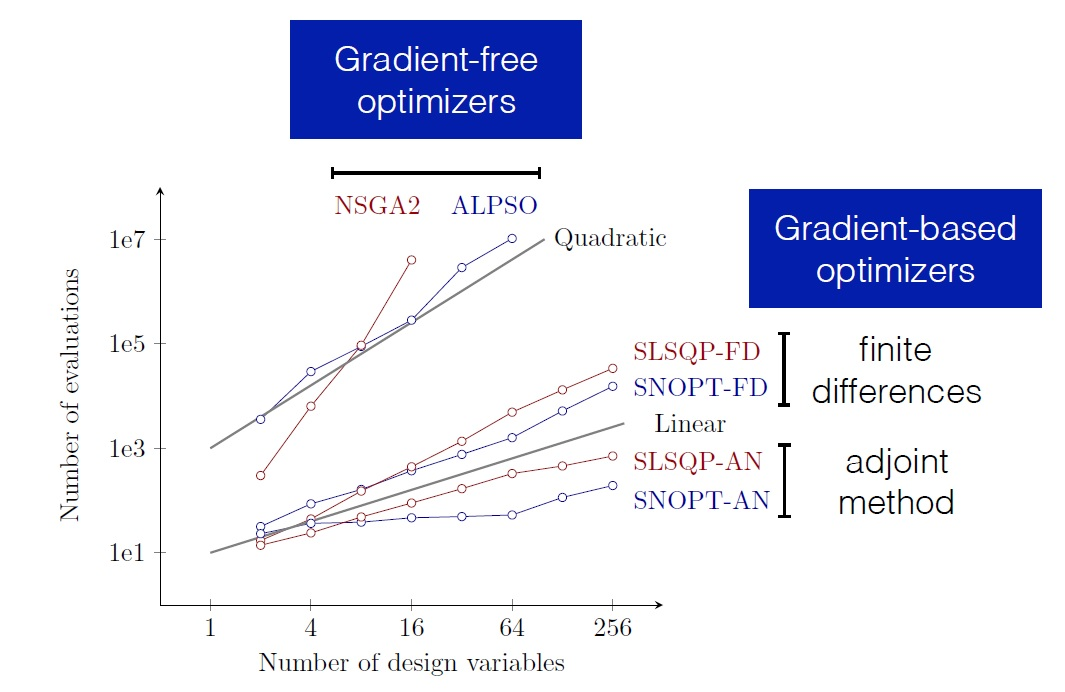
\includegraphics[keepaspectratio, width=0.8\textwidth]{images/chap2/gradbas_vs_gradfree.jpg}
	\caption{Comparison between gradient-free and gradient-based methods on the required number of iterations~\cite{bib:martins_2014}.}
	\label{fig:gradbas_vs_gradfree}
\end{figure}

The total derivatives compose a non linear system of equations which can be solved by an adjoint or a direct method. 
The solution of this system gives the path towards the function minimum. 
The usage of unified theory makes OpenMDAO perfect for large-scale problems, since it conjugates computational efficiency and multidisciplinary design~\cite{bib:hwang_omdao}. 
Also, as a consequence, the computational cost is kept low even increasing the number of disciplines in coupled high-fidelity problems~\cite{bib:martins_2005}. 
This is a key in the design of new technologies, such as BLI, since it enables to establish tradeoff in acceptable time. 

Starting from v2.4 the usage of sparse matrix has been implemented, reducing the computational cost to solve the non linear system of derivatives. 
Sparse matrices also allow to use a direct method, instead of a numerical one, in order to find the solution of the non linear system, making the code stable and easy to use by a user who does not have enough background on numerical methods, which is a non-trivial aspect.

The success of OpenMDAO as a reliable and efficient multidisciplinary optimisation platform is demonstrated by its large users community.
Problems concerning the aero-structural optimisation~\cite{bib:jasa_openaerostruct}, topology optimisation~\cite{bib:jasa_topology}, on-demand mobility~\cite{bib:hwang_x57}, small satellite design~\cite{bib:hwang_satellite}, trajectory optimisation with cost analysis~\cite{bib:hwang_mission_opt}, wind turbine blade shape optimisation~\cite{bib:barlas} and boundary layer ingestion optimisation using high fidelity~\cite{bib:gray} are succesfully solved with this framework.

In the following paragraphs, a brief description on how to use OpenMDAO is provided. 
In this manner, the integration of FAST can be better illustrated: more details about its structure, as well as the theory behind the solvers used and their implementation in the framework are given. 
OpenMDAO uses the object-oriented programming paradigm, which is facilitated by Python scripting, and an object composition design pattern. 
Just four classes are defined in OpenMDAO: \texttt{Component, Group, Driver}, and \texttt{Problem}.
They are detailed below. 

\begin{itemize}
	\item \texttt{Component} class. Components in OpenMDAO replace the classical definition of ``discipline'' in a MDO process. 
	They can represent a whole discipline, or a sub-set of it.
	Components share a common interface that allows them to be integrated to form larger problems: thus, they are the fundamental bricks in OpenMDAO to build the process.
	There are no specification about the component's instance: it simply maps a set of inputs to give a desired set of outputs, no matter if the outputs are provided with equations or a call to an external software, potentially written in a different language. 
	The \texttt{Component} class can be further divided into \texttt{ExplicitComponent} and \texttt{ImplicitComponent}: as the name suggests, the first uses explicit formulation in which the outputs are direct function of inputs; on the contrary in the second instance outputs are implicit function of inputs, and they are found through an iterative procedure that drives the function's residuals (defined by the user) to zero. 
	
	\item \texttt{Group} class. The \texttt{Group} instance contains the components, other groups, or a mix of both. 
	The relationship between groups and components forms a hierarchy tree, where a top-level group contains other groups. 
	In turn, these groups contain other groups and so on; the bottom-level contains only components. 
	There are no limit on the hierarchy level that can be defined. \texttt{Group} instances are used mainly to package sets of components together, to create better organised namespaces (since all the components are named based on their ancestors on the tree) and to facilitate the use of hierarchical nonlinear and linear solvers. 
	The ensemble of all the groups basically forms the model. 
	
	\item \texttt{Driver} class. The \texttt{Driver} instance defines a set of algorithms which iteratively call the model. 
	The algorithms are not only limited to optimisation, but can be also defined to execute other functionalities, \textit{i.e.} a sensitivity analysis or design of experiments.
	As said previously, \texttt{Driver} class already instances the \texttt{Scipyoptimisation} and the \texttt{pyOptSparse} classes, but a user can code its own class, which can be later instanciated in OpenMDAO. 
	In case of optimisation, design variables are a subset of models' inputs, objective function and eventually constraints are a subset of models' outputs. 
	
	\item  \texttt{Problem} class. This class has the function of top-level container, which includes all the objects defined. A \texttt{Problem} instance contains all the hierarchical structure, defined by groups and components, and a single driver instance. Aside of serving as a container, \texttt{Problem} class provides also the user interface for setup and execution.   
\end{itemize} 

The relationship between the four OpenMDAO classes is illustrated in Fig.~\ref{fig:omdao_class_relation}. Following the same definition given by Gray et al.~\cite{bib:gray_omdao}, ``partial derivative'' refers to the derivatives of component outputs with respect to inputs, meanwhile ``total derivative'' refers to derivatives of model outputs with respect to model inputs. 
\begin{figure}[!h]
	\centering
	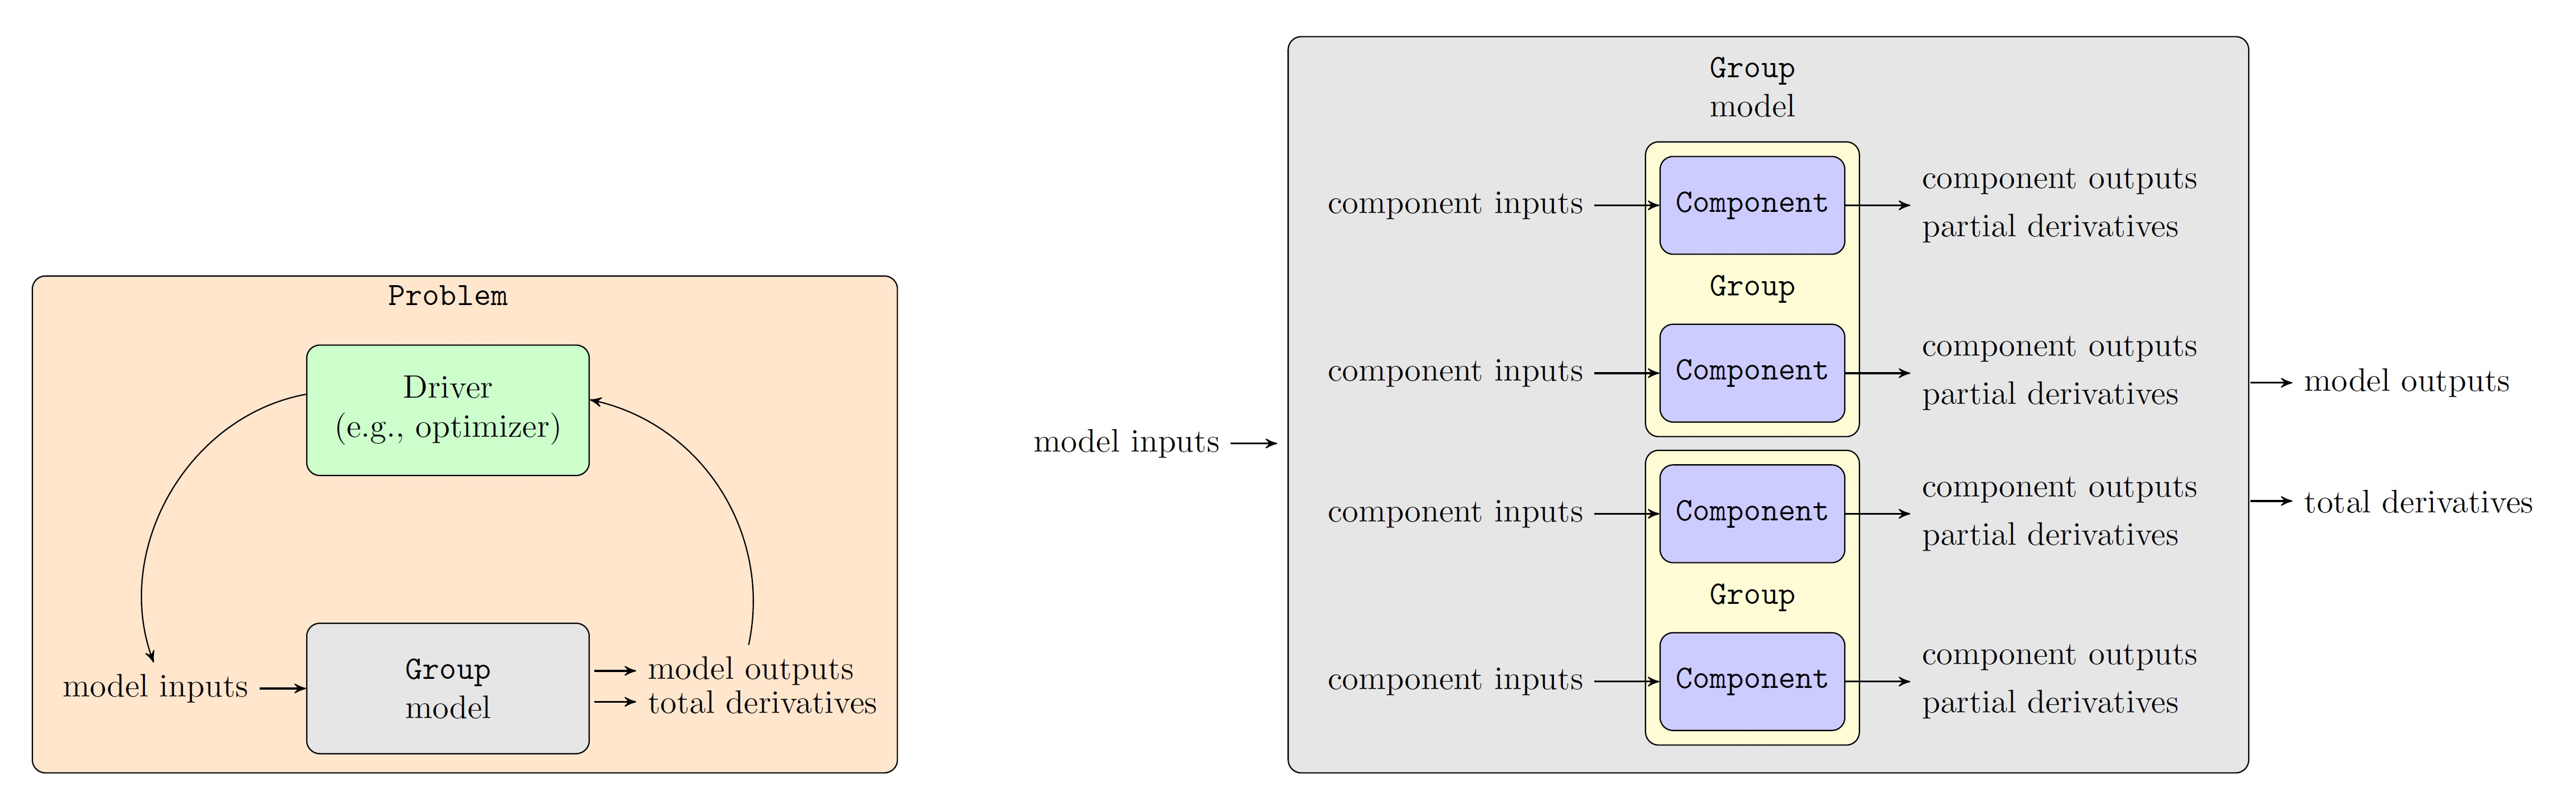
\includegraphics[keepaspectratio, width=\textwidth]{images/chap2/omdao_comp_relation.jpg}
	\caption{Relations between the OpenMDAO four basic classes: \texttt{Component, Group, Driver} and \texttt{Problem}~\cite{bib:gray_omdao}.}
	\label{fig:omdao_class_relation}
\end{figure}

Following this overview of OpenMDAO, the next step consists in detailing the integration of FAST within this optimisation platform. 

\section{The integrated plaftorm FAST and OpenMDAO}
\label{sec:chap2_fast_omdao_base}

To proceed with the integration of FAST and OpenMDAO, the disciplines must be rewritten in the OpenMDAO language, using components and groups.
For clarity, from now on the original version of FAST is referred as ``original version'' meanwhile the new one within the OpenMDAO platform is referred as ``integrated version''. 
One important difference is that under OpenMDAO, the integrated version carries out aircraft optimisation, starting from the same set of TLAR as the original version.
It must be noted that the optimisation can be carried out in other ways than using OpenMDAO, \textit{i.e.} using the gradient-free algorithms available in the \texttt{SciPy} library, or a global algorithm as SEGOMOE, jointly developed by ONERA and ISAE-Supaero~\cite{bib:bartoli_sego}.
These solutions are more intuitive and in some way simpler to implement than the complete OpenMDAO process. 
In this Ph.D., the choice has been to go with the recoding in OpenMDAO because of its various advantages, especially when dealing with derivatives, as seen from the description of previous section and the works that use OpenMDAO~\cite{bib:gray_omdao}. 
The use of derivatives has a major interest because the high efficiency of gradient-based methods, remarked also in Fig.~\ref{fig:gradbas_vs_gradfree}. 

For this reason it has been chosen to develop the integrated version of FAST considering derivatives information for aircraft optimisation.
This choice led to an imporant set-up time dedicated in the recoding of FAST under the OpenMDAO language. 
Because of this fully recoding, it has been decided to move from Python 2.7 to Python 3.7, which is a more recent and stable Python version. 

The starting point is then to convert all the disciplines as they are into \texttt{ExplicitComponent} or \texttt{ImplicitComponent}, according to their nature. 
Derivatives can be then computed with finite difference method. 
However, this is not the most efficient choice: except for some specific modules that call XFoil or OpenVSP, FAST is based on mathematical expressions: it is possible to have analytic derivatives, better in terms of required iterations (see again Fig.~\ref{fig:gradbas_vs_gradfree}). 
To facilitate their computation, each discipline has then been broken into small components, basically one \texttt{Component} instance (explicit or implicit) for each equation; subsequently all these elements have been regrouped again to form groups, each group representing a discipline, in agreement with the schema of Fig.~\ref{fig:fast_basic}.

At this stage of the process develoment, it is necessary to choose the MDO architecture: in fact the outputs definition depends on the architecture. 
Among all the possibilities, listed in the work of Martins and Lambe~\cite{bib:martins_mdo} and reported in Appendix~\ref{app:mdo_rev}, it has been decided to proceed with a Multidisciplinary Feasible (MDF) architecture, for several reasons, detailed here after:
\begin{itemize}
	
	\item It is the most intuitive to implement in the case of FAST, since the MDA loop is already defined. Also, since a recoding is necessary for the MDA, it allows to reduce the time dedicated to this phase, because it simply requires to add an optimiser at architecture top level;
	
	\item The main drawback of the MDF is that it requires a full MDA to be solved at each iteration~\cite{bib:martins_mdo}. However, because of the low CPU time for a sizing loop, this issue is not limiting;
	
	\item It requires the minor number of outputs definitions, since consistency constraints and residuals are not required;
	
	\item In case of optimisation failure before the convergence, it ensures consistency at each iteration, that is the aircraft is always consistent, albeit it may not be feasible from a constraints point of view.
	This feature may be useful for designers, because it is still possible to establish a tradeoff with design variables even if the optimisation fails, and facilitate the correction of the starting point. 
\end{itemize}

The xDSM diagram for the integrated version is shown in Fig.~\ref{fig:fast_openmdao_basic}, where the MDA loop within the MDF architecture is clearly identified. 
The equivalent algorithm is reported in Algorithm~\ref{alg:fast_openmdao_basic}.
In this schema, the engine deck initialization is explicited in this diagram (step 1).
\begin{figure}[!h]
	\centering
	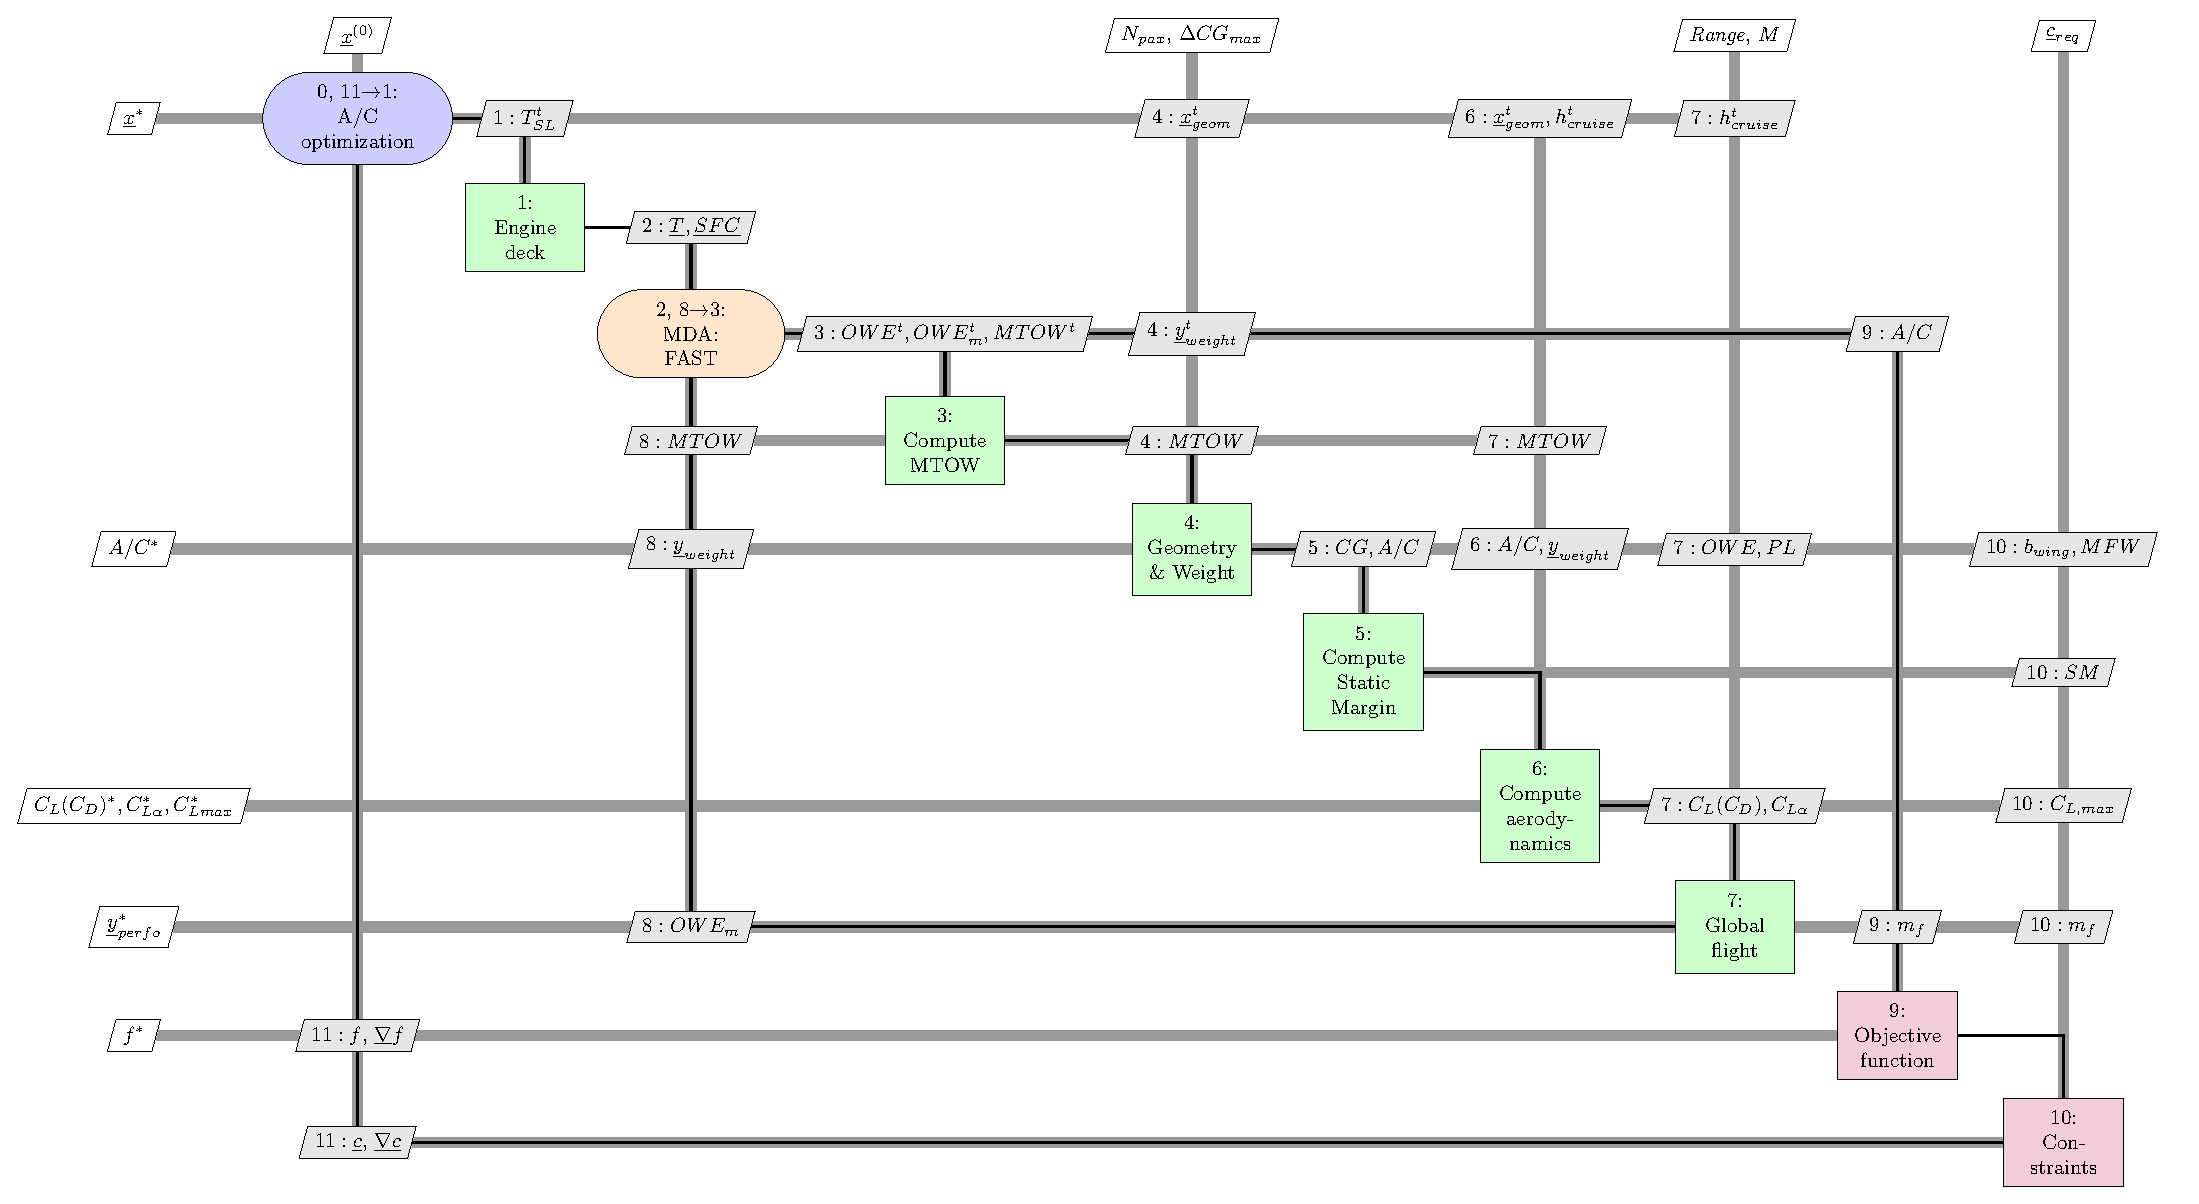
\includegraphics[keepaspectratio, width=1.3\textwidth, angle=90]{images/chap2/FAST_OpenMDAO_basic}
	\caption{xDSM diagram for the integrated version of FAST, obtained by the coupling with OpenMDAO.}
	\label{fig:fast_openmdao_basic}
\end{figure}
\begin{algorithm}[!h]
	\caption{Integrated version of FAST and OpenMDAO algorithm description, tailored to perform an optimisation of a conventional turbofan aircraft (integrated version).}
	\label{alg:fast_openmdao_basic}
	\begin{algorithmic}
		\REQUIRE Initial design parameters (TLAR), design variables initial vector $\underline{x}^{(0)}$
		\ENSURE Sized aircraft, drag polars, masses, performance, $\underline{x}^*$
		\STATE 0: Initialise the optimisation loop: initial values are read from the \texttt{xml} file.
		\REPEAT
		\STATE 1: Initialise the engine deck, using one of the models available, starting from the thrust at sea level.
		\STATE 2: Initialise the MDA (used to get a viable aircraft).
		\REPEAT
		\STATE 3: Compute MTOW.
		\STATE 4: Compute the aircraft geometry and perform the mass breakdown, to estimate weight of all components.
		\STATE 5: Compute the static margin, to check later on if the stability constraint is satisfied or not.
		\STATE 6: Aerodynamics calculation, based on the same equations of the original version.
		\STATE 7: Compute the aircraft performance.
		\STATE 8: Check the convergence. The driving parameter is the MTOW, when the error is lower than the tolerance, convergence is reached.
		\UNTIL {$8 \rightarrow 3$: MDA has converged}
		\STATE 9: Evaluate the objective function. If a gradient based solver is used, this analysis computes also derivatives.
		\STATE 10: Evaluate the design constraints. If a gradient based solver is used, this analysis computes also the derivatives of each constraint.
		\STATE 11: Check if the optimisation has converged. If not, this analysis updates $\underline{x}$ for the next iteration.
		\UNTIL {$11 \rightarrow 1$: MDO has converged}
	\end{algorithmic}
\end{algorithm}
The \texttt{xml} file is still used as I/O, but since the parameters need to be defined in OpenMDAO language, the meta-model GAMME is not used anymore. 
Instead, the dictionary is defined in Python, then an explicit component reads the \texttt{xml} and saves the values in the OpenMDAO format. 

Another consideration is that the optimisation must be ``fully opened'', in the sense that any of the chosen design variables must be constrained within a component, but it must be free to vary. 
The clearest example of this concept is the case of the wing area: in Sec.~\ref{subsubsec:chap2_fast_geom} it has been said that two values of wing area are computed, using Eq.~\eqref{eq:wing_approach_condition} and Eq.~\eqref{eq:wing_fuel_condition}, and then the maximum between the two is considered. 
In this way the design space for the wing area is limited to just two values, one for each condition to satisfy, where in real wing area can assume all the values included in an acceptable domain~\cite{bib:roskam_partI}. 
It may be that the optimal value for wing area is not one of the two explored, but another one contained in the design space.  
At the root of the optimisation logic, instead, there is the idea to define a design space exploration for each design variable.
Variables are then free to assume any value contained in its design space, it is up to the optimiser to find the optimal value that satisfies the design constraints. 

In the example of the wing area, with this logic Eq.~\eqref{eq:wing_approach_condition} and Eq.~\eqref{eq:wing_fuel_condition} are rewritten as inequalities:
\begin{equation}
	\label{eq:wing_constraint}
	\left\{\begin{array}{l}
			C_{L_{\max}} \geq \frac{m_{L}g}{\frac{1}{2}\rho V^2 S_{w}} \\
			224 S_{w}^{1.5}AR^{-0.4}\left[0.6\left(\frac{t}{c}\right)_{root}+0.4\left(\frac{t}{c}\right)_{tip}\right]+1570 \geq m_f
		\end{array}\right.
\end{equation}
Afterwards, the set of Eq.~\eqref{eq:wing_constraint} are added as design constraints, in order to let the wing area exploits all the possible values and find the optimal one that satisfies the conditions. 
The same approach applies also to the horizontal and vertical tails surface, as well as the wing position and the cruise altitude. 
In short, all the design rules that were hard coded in the original FAST, are now opened and threated as design constraints in an optimisation logic. 

As a result, the integrated version features less iterative loops than the original one: specifically the geometry module does not exhibit anymore a double loop, and concerning the performance calculations, the process does not need to iterate to find the cruise altitude. 
This can be also seen in Fig.~\ref{fig:fast_openmdao_basic_geom}, which shows the xDSM diagram for the new geometry module. 
It is clear that now the wing position is an input that serves for the SM calculation; the optimal value is chosen to minimize the objective function and to respect the SM constraints. 
\begin{figure}[!h]
	\centering
	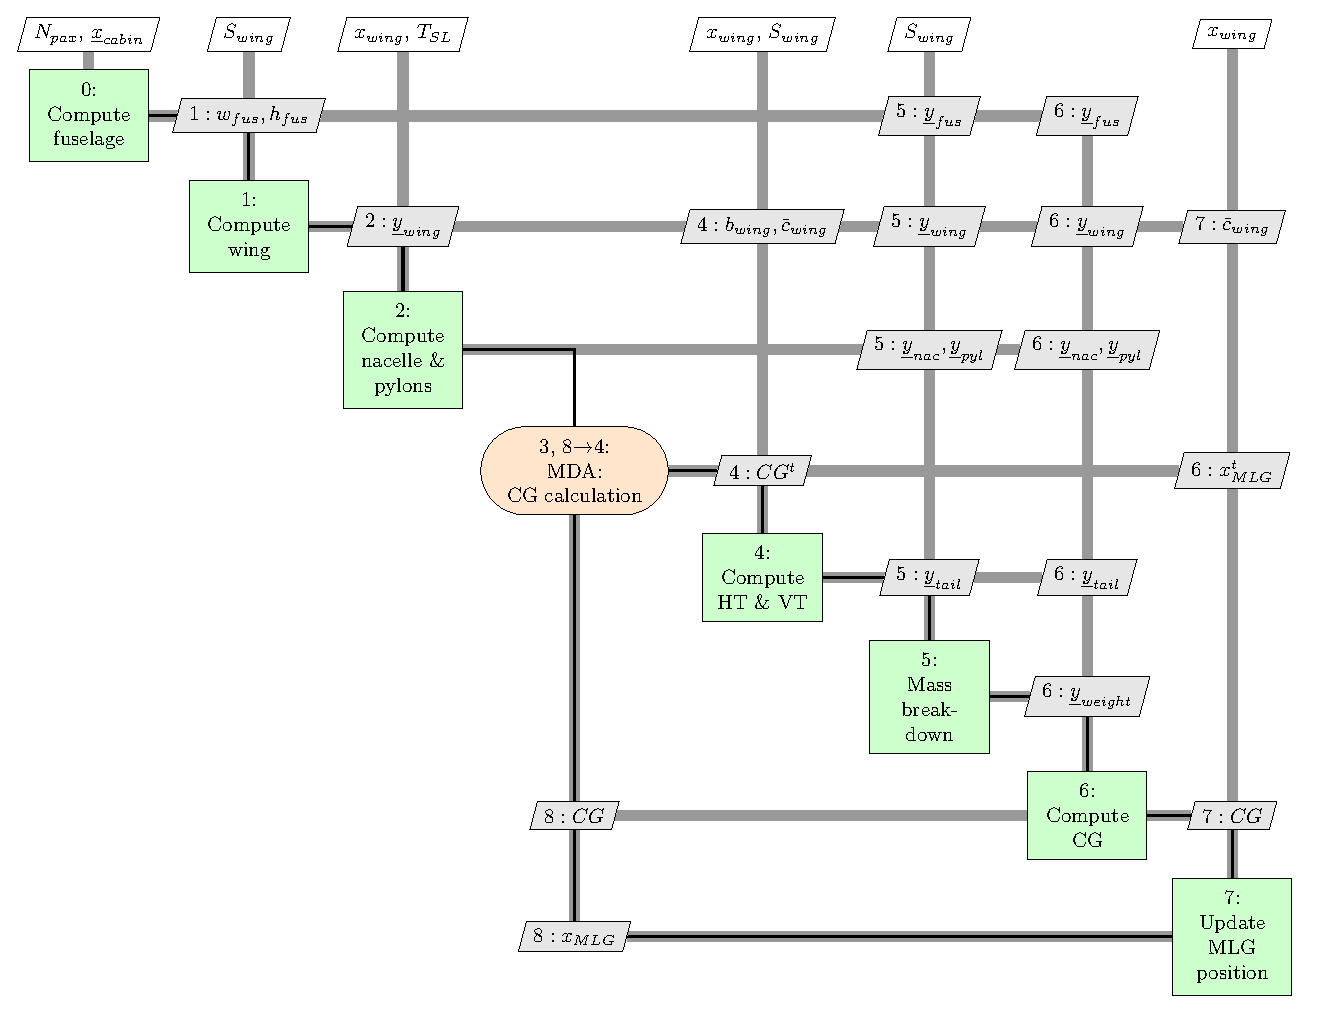
\includegraphics[keepaspectratio, width=\textwidth]{images/chap2/FAST_OpenMDAO_basic_geom}
	\caption{xDSM diagram for the geometry module of integrated version FAST and OpenMDAO.}
	\label{fig:fast_openmdao_basic_geom}
\end{figure}

Also, to fully open the problem, it has been decided to remove all the relationships between geometrical variables. 
As said in Sec.~\ref{subsubsec:chap2_fast_geom}, in fact, a lot of geometrical parameters, like the sweep of the tails, are related to the main wing parameters through statistical equations. 
From a design point of view, there are no reasons to keep these relations.
Thus and then all these parameters have been added as design variables, resulting in a larger design space exploration.

Regarding the performance analysis, beside the absence of the iterative loop to find the cruise altitude, the module is now more efficient because each mission segment has become an explicit component. 
This enables the possibility to recode the mission simulation in order to remove the issue found in the calling of descent function during the cruise leg. 
The integrated version just requires an initial guess of the distance to travel in cruise. 
Then, this value is iteratively changed until the total distance travelled for climb, cruise and descent is equals to the required range. 
With this modification, the descent component is called less than 10 times over a mission.
Compared to the hundred of times of original version that accounted for most of the computational cost, this change contributed strongly to the efficiency improvement of the process, with a reduction in time estimated in 5-10 minutes, as remarked at the end of Sec.~\ref{subsubsec:chap2_fast_perfo}. 

To consider certification specifications, the prescribed values reported in Table~\ref{tab:ccm_rules} are directly computed at the flight point of interest, since the CCM can not be used directly, having being coded using GAMME. 
However, the two formulations are totally equivalent. 
The certification conditions are then defined as design constraints, in order to let the optimiser find the optimal set of design variables that minimize the objective function, satisfying the CATPOL and CS-25 rules. 

Other minor considerations are related to the numerical schemes.
In the original version, for each iterative loop, the fixed point method was used.
In the integrated version it is possible to choose between a large variety of methods, available in OpenMDAO (like the Gauss-Seidel or the Krylov methods).
Also, robustness is increased: the original version needed to initialise the starting point because otherwise there was the risk to not get 
any results. 
OpenMDAO, instead, does not present any issue related to the choice of initial point; convergence is always ensured even with a bad choice of the initial point. 
Of course, if $\underline{x}^{(0)}$ is well chosen, the convergence is faster as the algorithm requires less iterations.

One of the possible risk of using OpenMDAO, from a user point of view, is the choice of a proper numerical scheme for convergence. 
In fact, a good choice can accelerate the convergence, but a background on numerical computation is needed~\cite{bib:leveque_partial_equation}. 
In OpenMDAO it is possible to directly solve the problem using a direct solver: it represents the easiest way since it always ensures the convergence.
On the other side it is costly since it requires a full matrix inversion~\cite{bib:gray_omdao}. 
However, starting by the v2.4, sparse matrices have been added to help the calculation. 
This results that a direct solver is efficient as a numerical scheme, which is an added feature for users. 
Finally, always related to robustness, it is worthy to note that thanks to the absence of convergence problems, the final tolerance in the integrated version is reduced of 3 orders of magnitude, from $10^{-3}$ to $10^{-6}$, resulting in more accurate results.

Despite these advantages, the integrated version presents a relevant drawback: in fact, there are more than 200 components to facilitate analytic gradient computation, compared to the 19 classes of the original one, making the code not user friendly to modifications by a new user, neither easy to understand and to use.
Also, due to the way the process is built, it is no more possible to use the code only for sizing, since parameters as wing area, wing position and so on are now design variables subject to design constraints.
In OpenMDAO, design constraints are not activated when a simple run is carried out, but they act only in an optimisation simulation. 

Also, in some cases it may be of interest to perform multiobjective optimisation, but OpenMDAO is limited to single objective problems when dealing with derivatives; from v2.4 it allows the use of NSGA-II, a genetic algorithm for multiobjective optimisation~\cite{bib:nsga2}, but it is gradient-free and thus requires long computational time. 
However, this issue can be handled with the definition of weighted functions~\cite{bib:chircop, bib:giagkiozis} or the development of specific algorithms~\cite{bib:desideri}. 
In Sec.~\ref{subsubsec:chap3_hybrid_pareto} and Sec.~\ref{subsec:chap4_bwb_pareto} examples are provided, in relations with the optimisation of the hybrid TAW and the BWB with DEP. 

The next paragraph states the optimisation problem, identifing the design variables as well as the constraints, and reports some results on the A320 CERAS validation case and a set of baseline aircraft.
These configurations will be use later on to assess performance of conventional configurations. 

\subsection{Optimisation of a turbofan aircraft with FAST under OpenMDAO}
\label{subsec:chap2_a320_optim_exploration}

\subsubsection{Problem formulation}
\label{subsubsec:chap2_a320_optim_prob_formulation}
This section presents an application of the new framework, built on the integration of FAST within OpenMDAO. 
At first, the problem must be defined: the main interest, for a civil transport aircraft, is to reduce the fuel consumption $m_f$.
This parameter becomes the objective function; all the geometrical inputs are now design variables. 
Also the cruise altitude and the thrust at sea level belongs to the design variables vector: the first is added because, in agreement with the original version, it is desired to have the aircraft always starting the cruise at the optimal altitude.
The second parameter instead allows to resize the engine according to thrust requirements. 
Finally, design constraint must be added. 
They need to ensure the feasibility of the concept, and also to comply with airport specification, top level requirements as well as certification (see Table~\ref{tab:ccm_rules}). 
The various constraints are listed below, with details to better explain the OAD problem. 
\begin{itemize}
	\item The wing has to carry all the fuel needed ($\Delta m_f = \textrm{MFW}-m_f\geq0$, being MFW the maximum fuel weight) and match the approach condition ($\Delta C_{L_{ldg}}=C_{L_{\max}}-C_{L_{app}}\geq0$).
	
	\item The horizontal tail is sized to obtain rotational performance at takeoff: the longitudinal momentum balance has to be larger than zero (zero at limit) for a given maximum center of gravity variation. This condition is defined by imposing that the total momentum is lower than zero $\Delta\mathcal{M}_{takeoff}\leq0$.
	
	\item The vertical tail is sized to have lateral stability in cruise: $S_{VT}$ has to ensure that the fuselage yaw moment is counterbalanced by the vertical tail yaw moment. 
	In mathematical symbols it can be written as $\Delta\mathcal{N}_{cruise}\geq0$, being $\mathcal{N}$ the yaw moment.
	
	\item The static margin SM has to be included between the 5\% and 10\% of the mean aerodynamics chord, in agreement with Eq.~\eqref{eq:static_margin_limits}. This condition determines the wing position $x_w$, which is placed to have SM in the required range.
	
	\item Wing span $b_w$ and takeoff field length TOFL are limited by aerodrome constraints for a medium range aircraft, in agreement with ICAO rules~\cite{bib:debarros, bib:icao}.
	
	\item The lift coefficient at the top of climb has to be equal to the value that maximizes the lift to drag ratio, to fly at the best altitude; in other words $\Delta C_{L_{toc}}=C_{L_{toc}}-C_{L_{opt}}=0$.
	
	\item The CATPOL~\cite{bib:catpol} and CS-25~\cite{bib:cs25} specifications must be satisfied as given in Table~\ref{tab:ccm_rules}. 
	In total, there are 6 constraints taken from the CCM; to simplify the process, these conditions have been collected in a single vector $$\underline{c}_{CCM}=[V_{z_{toc}}-300, V_{z_{tod}}-300, \gamma_{\%_{119a}}-3.2, \gamma_{\%_{121a}}, \gamma_{\%_{121b}}-2.4, \gamma_{\%_{121c}}-1.2, \gamma_{\%_{121d}}-2.1]$$ which must be greater than 0. 
\end{itemize}

With these notations, the problem formulation can be finally written: it is reported in Table~\ref{tab:a320_base_problem_optimisation_definition}, following the MDO community standard (see \textit{i.e.} the work of Jasa et al.~\cite{bib:jasa_topology}).
For each design variable, lower and upper bounds are defined, and this results in prescribing a design space. 
Limits are chosen recalling data on a large set of commercial single-aisle aircraft~\cite{bib:roskam_partII}. 
The size of the problem is 13, with 1 equality and 12 inequalities design constraints. 
\begin{table}[h!]
	\centering
	\begin{tabular}{l l r r r r l}
		\hline
		\textbf{Category} & \textbf{Name} & \textbf{Size} & \textbf{Lower} & \textbf{Upper} & \textbf{Equals} & \textbf{Units} \\
		\hline
		Objective & $m_f$ & 1 & -- & -- & -- & \si{\kilogram} \\
		\hline
		Variables & $S_w$ & 1 & \num{100} & \num{150} & -- & \si{\square\meter} \\
		& $x_w$ & 1 & \num{15} & \num{20} & -- & \si{\meter} \\
		& $AR_{w}$ & 1 & \num{8} & \num{12} & -- & -- \\
		& $\lambda_{w}$ & 1 & \num{0.2} & \num{0.6} & -- & -- \\
		& $\Lambda_{25_{w}}$ & 1 & \num{20} & \num{45} & -- & \si{\deg} \\
		& $\left(\frac{t}{c}\right)_w$ & 1 & \num{0.1} & \num{0.15} & -- & -- \\
		& $S_{HT}$ & 1 & \num{20} & \num{60} & -- & \si{\square\meter} \\
		& $AR_{HT}$ & 1 & \num{2} & \num{5} & -- & -- \\
		& $\lambda_{HT}$ & 1 & \num{0.2} & \num{0.6} & -- & -- \\
		& $\Lambda_{25_{HT}}$ & 1 & \num{20} & \num{45} & -- & \si{\deg} \\
		& $\left(\frac{t}{c}\right)_{HT}$ & 1 & \num{0.1} & \num{0.15} & -- & -- \\
		& $S_{VT}$ & 1 & \num{15} & \num{50} & -- & \si{\square\meter} \\
		& $AR_{VT}$ & 1 & \num{1} & \num{2.5} & -- & -- \\
		& $\lambda_{VT}$ & 1 & \num{0.3} & \num{1.0} & -- & -- \\
		& $\Lambda_{25_{VT}}$ & 1 & \num{25} & \num{55} & -- & \si{\deg} \\
		& $\left(\frac{t}{c}\right)_{VT}$ & 1 & \num{0.13} & \num{0.18} & -- & -- \\
		& $T_{SL}$ & 1 & \num{90} & \num{130} & -- & \si{\kilo\newton} \\
		& $h_{toc}$ & 1 & \num{30000} & \num{40000} & -- & ft \\
		& \textbf{Total} & 18 & & & & \\
		\hline
		Constraints & $\Delta m_{f}$ & 1 & 0 & -- & -- & \si{\kilogram} \\
		& $\Delta C_{L_{app}}$ & 1 & 0 & -- & -- & -- \\
		& $b_w$ & 1 & -- & \num{36} & -- & \si{\meter} \\
		& $\mathcal{M}_{takeoff}$ & 1 & -- & \num{0} & -- & \si{\newton\meter}  \\
		& $\Delta \mathcal{N}_{cruise}$ & 1 & \num{0} & -- & -- & \si{\newton\meter} \\
		& TOFL & 1 & -- & \num{2200} & -- & \si{\meter} \\
		& $\Delta C_{L_{toc}}$ & 1 & -- & -- & 0 & -- \\
		& SM & 1 & \num{0.05} & \num{0.10} & -- & -- \\
		& $\underline{c}_{CCM}$ & 5 & \num{0} & -- & -- & \% \\
		& \textbf{Total} & 13 & & & & \\
		\hline    	
	\end{tabular} 
	\caption{Optimisation problem definition for the A320 CERAS case. Variables' limits come from literature review on single aisle type aircraft~\cite{bib:roskam_partII}.}
	\label{tab:a320_base_problem_optimisation_definition}
\end{table}

\subsubsection{Test case: A320 CERAS aircraft}
\label{subsubsec:chap2_a320_optim_ceras}

The first test case to be analysed is the optimisation of the A320 CERAS aircraft, already studied with the original version of FAST in Section~\ref{subsec:chap2_fast_test_case}, associated to TLAR reported in Table~\ref{tab:fast_base_tlar}. 
One issue regarding gradient-based methods is that the optimum point $\underline{x}^*$ can be a local minimum~\cite{bib:martins_mdo}.
To increase the likelihood of convergence to the global optimum, a multistart check is performed, with 10 different initial vectors $\underline{x}^{(0)}$.
If $\underline{x}^*$ does not depend on initial value, then it is assumed as global minimum; otherwise it is reasonable to consider that the global minimum is within the obtained solutions.
The 10 starting points are chosen through the creation of a Latin hypercube sampling LHS~\cite{bib:sacks}. 

Table~\ref{tab:optimisation_setup} reports the set-up that is used: the optimisation solver is SNOPT~\cite{bib:snopt}, a sequential least squares programming algorithm, that derives from SLSQP algorithm~\cite{bib:slsqp}, and included in the \texttt{pyOptSparse} library. 
It has been chosen because it is one of the most efficient gradient based algorithm (see also Fig.~\ref{fig:gradbas_vs_gradfree}), that supports both inequalities and equalities constraints~\cite{bib:snopt}. 
Linear and non-linear solver are respectively the Gauss--Seidel and the direct solver.
The utilisation of direct solver in place of a numerical method is justified by the consideration done in Sec.~\ref{sec:chap2_openmdao_overview}.
Starting from OpenMDAO 2.4, the implementation of sparse matrices makes the two methods comparable in terms of performance. 
Direct solver facilitates the setting, since it does not require the definition of pre-conditioner or similar options, and thus it is considered in this optimisation problem. 
Tolerance, both for MDA and MDO, is $10^{-6}$ as default value. 
\begin{table}[!h]
	\centering
	\begin{tabular}{l r}
		\hline
		\textbf{optimisation solver} & SNOPT \\
		\textbf{Linear solver} & Linear Gauss-Seidel \\
		\textbf{Non linear solver} & Direct solver \\
		\textbf{MDA tolerance} & $10^{-6}$ \\
		\textbf{optimisation tolerance} & $10^{-6}$ \\
		\hline
	\end{tabular}
	\caption{Set-up for the A320 CERAS optimisation problem, using gradient based method.}
	\label{tab:optimisation_setup}
\end{table}

Table~\ref{tab:a320_base_optim_comparison} reports a comparison between the quantities of interest for the considered test case, both for baseline and optimised aircraft, meanwhile Table~\ref{tab:a320_base_optim_dv} reports the design variables values.
The geometrical input parameters for the baseline are the same of Table~\ref{tab:fast_base_geom_inp}.
Note that most of the variables of Table~\ref{tab:a320_base_optim_dv} are computed within the original version with statistical equations, meanwhile in the integrated version they are free to vary within their specified range.
The mission profile is defined by using values of Table~\ref{tab:fast_base_thrust_rate_entry} for thrust setting. 
\begin{table}[!h]
	\centering
	\begin{tabular}{l l c c}
		\hline
		& & \textbf{Baseline} & \textbf{optimised} \\
		\hline
		\textbf{MTOW} & [\si{\tonne}] & 74.2 & 73.7 \\
		\textbf{OWE} & [\si{\tonne}] & 42.2 & 42.4 \\
		\textbf{Wing area} & [\si{\square\meter}] & 122.74 & 123.38 \\
		\textbf{Max. LoD} & & 15.9 & 17.1 \\
		\textbf{Static margin} & & 0.10 & 0.05 \\
		\textbf{Fuel mission} & [\si{\tonne}] & 18.7 & 17.1 \\
		\hline
		\textbf{CAT.POL.A.410(a)-1} & [ft/min] & 964.69 & 913.17 \\
		\textbf{CAT.POL.A.410(a)-2} & [ft/min] & 1031.82 & 663.85 \\
		\textbf{CS-25.119(a)} & [\%] & 19.46 & 17.82 \\
		\textbf{CS-25.121(a)} & [\%] & 1.61 & 2.01 \\
		\textbf{CS-25.121(b)} & [\%] & 3.43 & 2.47 \\
		\textbf{CS-25.121(c)} & [\%] & 5.56 & 5.30 \\
		\textbf{CS-25.121(d)} & [\%] & 7.19 & 6.78 \\
		\hline
	\end{tabular}
	\caption{Comparison between quantities of interest for the baseline and the optimised aircraft, A320 CERAS test case. Top level requirements are reported in Table~\ref{tab:fast_base_tlar}.}
	\label{tab:a320_base_optim_comparison}
\end{table}

\begin{table}[!h]
	\centering
	\begin{tabular}{l l c c}
		\hline
		& & \textbf{Baseline} & \textbf{optimised} \\
		\hline
		$S_w$ & [\si{\square\meter}] & 122.74 & 123.38  \\
		$x_w$ & [\si{\meter}] & \num{16.61} & \num{15.94}  \\
		$AR_{w}$ & & 9.5 & 10.6 \\
		$\lambda_{w}$ & & 0.38 & 0.33 \\
		$\Lambda_{25,w}$ & [\si{\deg}] & 25 & 23.4  \\
		$\left(\frac{t}{c}\right)_w$ & & 0.128 & 0.117\\
		$S_{HT}$ & [\si{\square\meter}] & 33.28 & 29.32  \\
		$AR_{HT}$ & & 43.28 & 3.74  \\
		$\lambda_{HT}$ & & 0.4 & 0.2  \\
		$\Lambda_{25,HT}$ & [\si{\deg}] & 28 & 32.14  \\
		$\left(\frac{t}{c}\right)_{HT}$ & & 0.1 & 0.1 \\
		$S_{VT}$ & [\si{\square\meter}] & 29.53 & 26.23  \\
		$AR_{VT}$ & & 1.74 & 1.2 \\
		$\lambda_{VT}$ & & 0.3 & 0.3  \\
		$\Lambda_{25,VT}$ & & [\si{\deg}] 35 & 35  \\
		$\left(\frac{t}{c}\right)_{VT}$ & & 0.1 & 0.1  \\
		$T_{SL}$ & [\si{\kilo\newton}] & 117.8 & 108.2  \\
		$h_{toc}$ & [ft] & 34000 & 33248  \\
		\hline
	\end{tabular}
	\caption{Comparison between design variables for the A320 CERAS test case baseline and optimised. Geometric inputs for the baseline are in agreement with Table~\ref{tab:fast_base_geom_inp}.}
	\label{tab:a320_base_optim_dv}
\end{table}

The first point to note is that the aspect ratio is increased. 
The optimiser finds that the optimal path goes towards a larger wing, that uses all the span possible (36~\si{\meter}).
As a result, the maximum lift-to-drag ratio is increased of about 8\%.
Also the OWE is slightly higher, because of bigger wing. 
However, the aerodynamics benefits overcome the penalties in weight, and the fuel consumption is reduced of about 9\%. 
This also results in a reduced MTOW. 
Another difference lies in the static margin: the original version, indeed, was coded in order that the internal loop stops the first time the static margin stays within the range of 5-10\%. 
This means that, if the initial wing position is backwarded, the SM achieved is always 0.10. 
In the integrated version, instead, the optimiser finds the most forwarded position, in order to increase tail level arm and to reduce the tail size. 
Also, aspect ratio and sweep of the horizontal tail are optimised to move the aerodynamics center in the farest position as possible, always to advance the wing the most allowable. 

Table~\ref{tab:a320_base_optim_comparison} reports also the values achieved for the various certification constraints during the sizing loop. 
It is interesting to note that the thrust of the engine is reduced while complying with the CS-25.121(b).
The reduction in thrust contributes to the increase in maximum lift-to-drag ratio too, since the engine wetted area is reduced. 

These results show that the problem is well-posed, and that the optimiser goes towards the best solution. 
Also, it is verified that with the 10 multistart approach, there are no local minima. 
In order to understand the presence of more minima, the objective function value and the norm of constraints are evaluated.
Considering the constraint written in the form $\underline{c}=[g_i\left(\underline{x}\right)-a_i]\leq0$, with $i=1,\cdots,N$, this last quantity is defined as: 
\begin{equation}
	\label{eq:norm_constraint}
	\Vert \underline c \Vert = \sum_{i=0}^{N}\vert g_i\left(\underline{x}\right)-a_i \vert
\end{equation}
where 
\begin{equation}
	\label{eq:sum_violation_constraint}
	\vert g_i\left(\underline{x}\right)-a_i \vert = \left\{
	\begin{array}{l l}
		0 & g_i\left(\underline{x}\right) \leq a_i + \epsilon \\
		g_i\left(\underline{x}\right)-a_i & \textrm{otherwise}
	\end{array} \right.
\end{equation}
with $\epsilon$ being the tolerance.
In other word, if a constraint is violated the norm is computed as the difference with respect to the minimum value, otherwise it is set to zero. 
As a consequence, a feasible point has the norm of the constraints equals to zero. 

Table~\ref{tab:a320_base_optim_multipoint_result} reports the final objective function $f^\star$ and the norm of constraints for the 10 runs: all the points are feasible, and no local minima are detected, since the maximum difference among the 10 $f^\star$ is less of 0.4\%.
\begin{table}[!h]
	\centering
	\begin{tabular}{l c c c c c c c c c c}
		\cline{2-11}
		& \multicolumn{10}{c}{\textbf{Run}} \\
		\cline{2-11}
		& 1 & 2 & 3 & 4 & 5 & 6 & 7 & 8 & 9 & 10 \\
		\hline
		$f^\star$ & 17094 & 17151 & 17086 & 17092 & 17139 & 17101 & 17089 & 17128 & 17112 & 17104 \\
		$\Vert \underline c \Vert$ & 0 & 0 & 0 & 0 & 0 & 0 & 0 & 0 & 0 & 0\\
		\hline
	\end{tabular}
	\caption{Objective function and norm constraints, defined as in Eq.~\eqref{eq:sum_violation_constraint}, for the 10 optimisation runs carried out for A320 CERAS test case baseline.}
	\label{tab:a320_base_optim_multipoint_result}
\end{table}

The payload-range is also computed with the integrated process: a comparison between the baseline and the optimised aircraft is shown in Fig.~\ref{fig:a320_base_optim_pl_range}. 
Only minor differences are detected: because of the reduced MTOW, the first horizontal segment is shorter, but then better aerodynamics and larger fuel capacity make the ferry range of the aircraft higher, even if the difference is of only few nautical miles. 
\begin{figure}[!h]
	\centering
	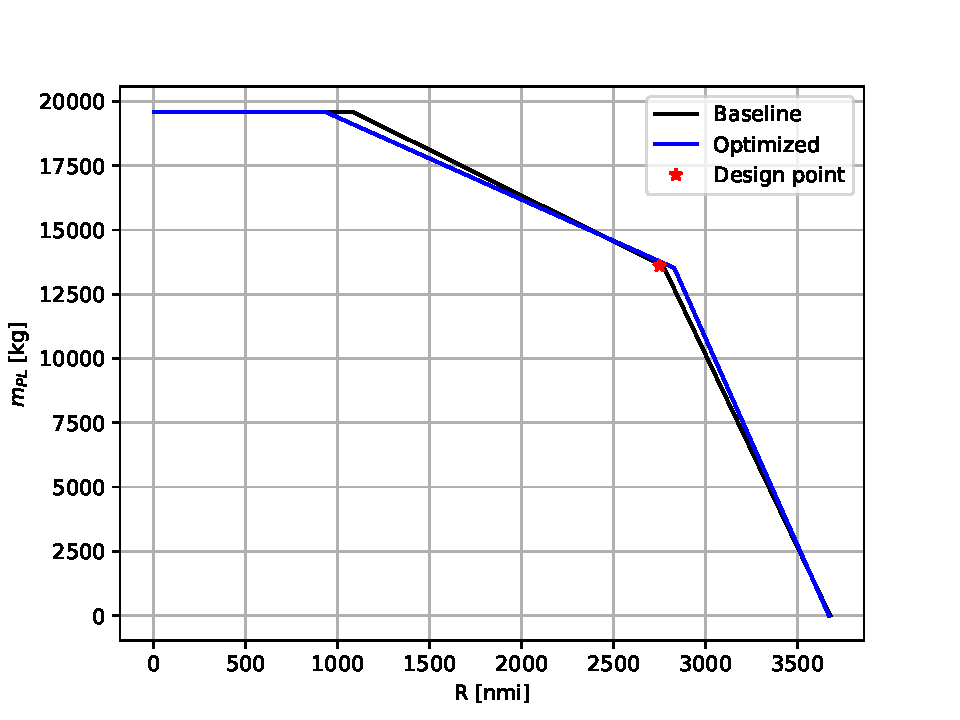
\includegraphics[keepaspectratio, width=0.6\textwidth]{images/chap2/fast_base_optim_pl_range}
	\caption{Payload-Range diagram, for the A320 CERAS test case, baseline and optimised aircraft.}
	\label{fig:a320_base_optim_pl_range}
\end{figure}

The code took about 35~\si{\minute} to reach the convergence; a total of 36 iterations, with 39 call to objective functions, have been needed to find the solution. 
The convergence history is shown in Fig.~\ref{fig:a320_optim_conv_history}. 
The algorithm finds very soon the minimum: indeed after 20 iterations, variations are so small that the objective value can be assumed constant. 
Note that up to iteration 10 the objective function is smaller than the final value, but these points do not respect the full set of design constraints and are not feasible. 
\begin{figure}[!h]
	\centering
	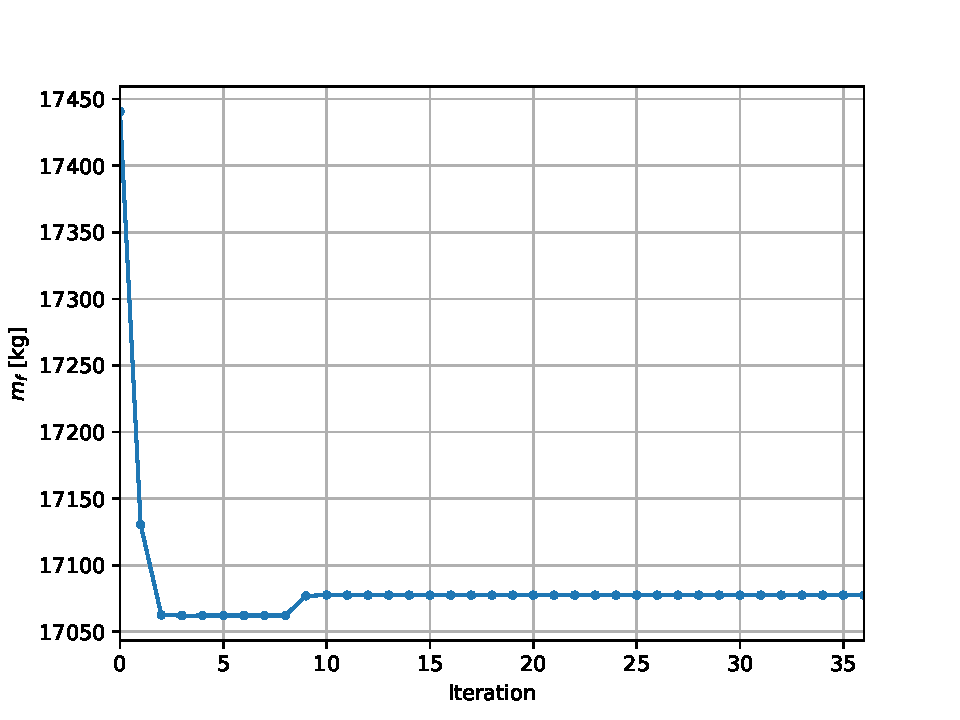
\includegraphics[keepaspectratio, width=0.6\textwidth]{images/chap2/fast_optim_conv_history}
	\caption{Convergence history for optimisation problem of A320 CERAS test case.}
	\label{fig:a320_optim_conv_history}
\end{figure}

\subsubsection{Test case: A320 CERAS resized for EIS2035}
\label{subsubsec:chap2_a320_optim_eis2035}

In this section, the integrated code is used to generate the baseline aircraft to be used as comparison for the assessment of unconventional configurations.
The technological horizon is 2035, which means that some assumptions have to be made for the mass estimation, the engine model and aerodynamics. 
The TLAR are practically the same, except for the range, that not 2750~nmi anymore. 
Its variation is instead limited from 600 to 1500~nmi.
This choice is dictated by the marketing.
According to an Airbus analysis, in fact, most of the aircraft fly in this operational range, and thus for the future can be considered to have new resized aircraft on these ranges~\cite{bib:airbus_global_market}. 
For clarity, the new TLAR are reported in Table~\ref{tab:a320_2035_tlar}. 
The mission profile is still the one of the A320 CERAS reference aircraft, presented in Table~\ref{tab:fast_base_thrust_rate_entry}. 
\begin{table}[!h]
	\centering
	\begin{tabular}{l r r}
		\hline
		Range & 600--1500 & nmi \\
		Number of passengers & 150 & \\
		Approach speed & 132 & \si{\knot} \\
		Design payload & 13608 & \si{\kilogram} \\
		\hline		
	\end{tabular}
	\caption{Top level requirements for the resized A320, considering EIS2035.}
	\label{tab:a320_2035_tlar}
\end{table} 

For the technological assumptions, the most reliable document available so far in literature is the IATA report~\cite{bib:iata, bib:iata_annex}, which states perspectives of available technologies in a 20 year period and their foreseen impact. 
Regarding the mass estimation, the use of innovative materials, like new alloys or composites, reduces the weight of the aircraft. 
The estimated impact of new technologies is reported in Table~\ref{tab:2035_mass_impact}. 
\begin{table}[!h]
	\centering
	\begin{tabular}{l c}
		\hline
		\textbf{Component} & \textbf{Impact on mass} \\
		\hline
		Wing & -10\% \\
		Fuselage & -5\% \\
		Landing gear & -15\% \\
		Pylons & -10\% \\
		Passenger seats & -60\% \\
		\hline
	\end{tabular}
	\caption{Impact of new technologies on airframe mass estimation according to IATA~\cite{bib:iata_annex}, considering EIS2035.}
	\label{tab:2035_mass_impact}
\end{table}
These estimations are not the only one available in literature, however they seem to be the more reasonable in the chosen technological horizon. 
The gains at discipline or component level have been implemented through the corrective factors technique, as described in Section~\ref{sec:chap2_fast_base_description}. 

For aerodynamics, improvements can be foreseen thanks to the introduction of different new technologies~\cite{bib:iata_annex}: 
\begin{itemize}
	\item \textbf{New winglet design}. A careful winglet design, with innovative and optimised shape, could lead to a reduction on the induced drag up to 10\%.
	
	\item \textbf{Laminarity drag coating}. The use of a film coating on the wing can reduce the roughness in order to achieve a fully laminar flow and reduce the friction coefficient up to 20\%. In practice, it is very sensitive to external condition and it is not said that the flow will be in any condition laminar.
	
	\item \textbf{Turbulent drag coating}. This technology is complementary to the previous one. A rough coating is added on the wing to induce turbulence: despite the flow results more viscous, the turbulence avoids separation and its impact on the $C_{D_{0}}$ is estimated to be of 5\%. Also, it is less sensitive to external condition than the laminarity drag coating.
	
	\item \textbf{Natural laminar flow control}. An accurate wing design can be achieved to naturally have laminar flow over the wing. In practice, this solution is unfeasible for wing with sweep angles higher than 20~\si{\degree}. 
	
	\item \textbf{Shock contol}. This technology uses a bump over the wing to control the shock wave geometry even in off-design conditions. 
	It may reduce the wave drag coefficient up to 50\%.
	
	\item \textbf{Morphing wing}. The idea at the back of this technology is to use smart materials that change the wing shape, in order to always adapt the geometry to external condition and increase the aerodynamics efficiency. 
	Its reduction on the total drag coefficient is estimated to be of about 3.2\%. 
	
	\item \textbf{Hybrid laminarity flow control (HLFC)}. In this case, laminarity is achieved throught both accurate wing design and active flow control to ingest boundary layer. Its effect on the friction coefficient is about 45-50\%. In practice the system introduces relevant penalties in weight, that may counterbalance the aerodynamics benefits. Also, its integration within the airframe is very challenging. 
\end{itemize}
For the 2035 reference aircraft, new winglet design, shock control and morphing wing are considered. 
The turbulent drag coating is also taken into in spite of the laminarity drag coating, because it is less sensitive to external condition and then more reliable. 
A natural shock control is unfeasible because of the transonic region, which requires a swept wing. 
Finally, HLFC is not considered because of limited knowledge at this stage: low maturity and penalties assessment are complex to quantify and it can introduce potential risks to the design. 

The final impacts on aerodynamics are reported in Table~\ref{tab:2035_aero_impact}.
As for the weight, variations have been implemented using corrective factors in Eq.~\eqref{eq:cd_total}. 
\begin{table}[!h]
	\centering
	\begin{tabular}{l c c}
		\hline
		\textbf{Technology} & \textbf{Parameter} & \textbf{Impact} \\
		\hline
		Winglet design & $C_{D_{i}}$ & -10\% \\
		Turbulent drag coating & $C_{D_{0}}$ & -5\% \\
		Shock control & $C_{D_{c}}$ & -50\% \\
		Morphing wing & $C_D$ & -3.2\% \\
		\hline
	\end{tabular}
	\caption{Impact of new technologies on aerodynamics according to IATA~\cite{bib:iata_annex}, considering EIS2035.}
	\label{tab:2035_aero_impact}
\end{table}

Some assumptions at engine level have also to be made. 
It is reasonable to consider that engines in the future will belong to ultra by-pass ratio category, as for the LEAP engine~\cite{bib:leap_engine}: these engines have a greater BPR, to increase the thrust generated by cold flow and consequently reduce the SFC. 
Current technology shows a maximum BPR of 11-12. 
It is foreseen that this value shall not be exceeded, to keep fan dimensions within the limits, but the engine improvements will be mainly related to a more efficient combustion process. 
To match 2035 assumptions, a BPR equals to 11 is taken into account, to have the effect of wetted areas, together with a reduction of SFC and an impact on the masses, due to a combined effect of larger engines and new materials. 

With these assumptions, it is finally possible to proceed with the sizing of a new set of A320 type aircraft, that matches the EIS2035. 
Again, the optimised aircraft is compared with some baseline, obtained with the original version using the geometrical input of Table~\ref{tab:fast_base_geom_inp}. 

The fuel consumption as a function of the design range is shown in Fig.~\ref{fig:a320_2035_optim_comp}, for the baseline and the optimised aircraft. 
For completeness, key parameters for each configuration are reported in Table~\ref{tab:a320_2035_non_optim_res} (baseline) and Table~\ref{tab:a320_2035_optim_res} (optimised). 
The optimised configuration shows a fuel saving in the order of 10-15\%; also since the slope of the curve of Fig.~\ref{fig:a320_2035_optim_comp} is lower for optimised aircraft, it can be expected that the impact will be greater on longer range. 
Same considerations done for the optimum point in Section~\ref{subsubsec:chap2_a320_optim_ceras} can be retaken here. 
Concerning certification constraints, for shorter range aircraft it is important to note that the sizing condition for the thrust is not anymore the slope at 400~ft of altitude, corresponding to CS-25.121(b), but more the CAT.POL.A.410(a)-2, which corresponds to the vertical speed reserve at the top of descent. 
This can be explained because the aircraft is more efficient, and therefore consumes less fuel. 
So the difference in weight between the beginning and the end of the cruise is reduced, and due to the higher mass it needs more thrust at the top of descent to match the needed $V_z$. 
On the other hand, condition CS-25.121(b), which was the most stringent condition in the case of Table~\ref{tab:a320_base_optim_comparison}, decreases with respect to range, so it can be expected that on longer range, where also the aircraft is lightened more because of the greater distance, it will be again the sizing condition for maximum thrust, in agreement with previous case. 
\begin{figure}[!h]
	\centering
	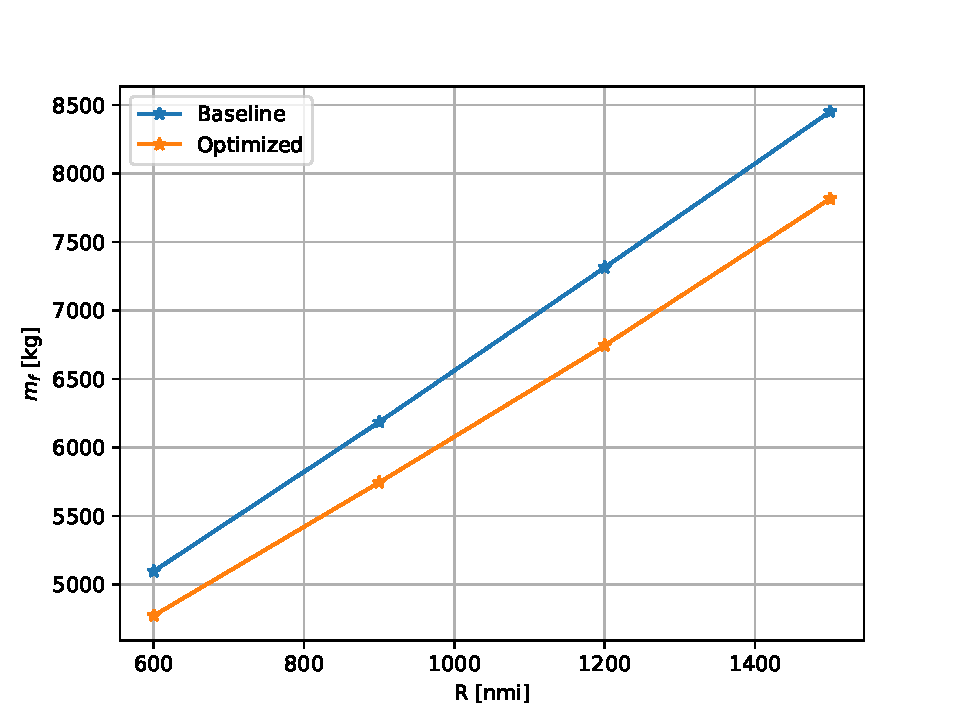
\includegraphics[keepaspectratio, width=0.6\textwidth]{images/chap2/fast_base_optim_comp}
	\caption{Fuel consumption as a function of design range for the A320 baseline and the optimised aircraft, resized to match EIS2035. TLAR are reported in Table~\ref{tab:a320_2035_tlar}. }
	\label{fig:a320_2035_optim_comp}
\end{figure}

\begin{table}[!h]
	\centering
	\begin{tabular}{l l c c c c}
		\cline{3-6}
		& & \multicolumn{4}{c}{\textbf{Range} [nmi]} \\
		& & \textbf{600} & \textbf{900} & \textbf{1200} & \textbf{1500} \\
		\hline
		\textbf{MTOW} & [\si{\tonne}] & 58.83 & 60.02 & 61.24 & 62.48 \\
		\textbf{OWE} & [\si{\tonne}] & 40.21 & 40.31 & 40.4 & 40.49  \\
		\textbf{Wing area} & [\si{\square\meter}] & 118.79 & 118.97 & 119.16 & 119.35 \\
		\textbf{Max. LoD} & & 17.44 & 17.44 & 17.43 & 17.43 \\
		\textbf{Fuel mission} & [\si{\tonne}] & 5.09 & 6.18 & 7.31 & 8.45 \\
		\hline
		\textbf{CAT.POL.A.410(a)-1} & [ft/min] & 932.18 & 929.41 & 928.88 & 927.4 \\
		\textbf{CAT.POL.A.410(a)-2} & [ft/min] & 786.4 & 780.39 & 774.13 & 767.66 \\
		\textbf{CS-25.119(a)} & [\%] & 21.98 & 21.92 & 21.87 & 21.81 \\
		\textbf{CS-25.121(a)} & [\%] & 6.01 & 5.65 & 5.31 & 4.97 \\
		\textbf{CS-25.121(b)} & [\%] & 7.94 & 7.64 & 7.28 & 6.91 \\
		\textbf{CS-25.121(c)} & [\%] & 8.84 & 8.57 & 8.29 & 8.05 \\
		\textbf{CS-25.121(d)} & [\%] & 8.8 & 8.76 & 8.72 & 8.68 \\
		\hline
	\end{tabular}
	\caption{Quantities of interest for the A320 case baseline, resized to match EIS2035 with TLAR reported in Table~\ref{tab:a320_2035_tlar} and geometrical inputs as in Table~\ref{tab:fast_base_geom_inp}.}
	\label{tab:a320_2035_non_optim_res}
\end{table}

\begin{table}[!h]
	\centering
	\begin{tabular}{l l c c c c}
		\cline{3-6}
		& & \multicolumn{4}{c}{\textbf{Range} [nmi]} \\
		& & \textbf{600} & \textbf{900} & \textbf{1200} & \textbf{1500} \\
		\hline
		\textbf{MTOW} & [\si{\tonne}] & 56.76 & 57.89 & 59.01 & 60.14 \\
		\textbf{OWE} & [\si{\tonne}] & 38.58 & 38.71 & 38.79 & 38.84  \\
		\textbf{Wing area} & [\si{\square\meter}] & 116.21 & 116.47 & 116.63 & 116.76 \\
		\textbf{Max. LoD} & & 18.47 & 18.46 & 18.45 & 18.44 \\
		\textbf{Thrust @ SL} & [\si{\kilo\newton}] & 99.5 & 100 & 100 & 99.75 \\
		\textbf{Fuel mission} & [\si{\tonne}] & 4.77 & 5.74 & 6.77 & 7.81 \\
		\hline
		\textbf{CAT.POL.A.410(a)-1} & [ft/min] & 905.76 & 905.59 & 904.13 & 904.48 \\
		\textbf{CAT.POL.A.410(a)-2} & [ft/min] & 308.9 & 315.24 & 309.41 & 300.24 \\
		\textbf{CS-25.119(a)} & [\%] & 17.54 & 17.61 & 17.57 & 17.49 \\
		\textbf{CS-25.121(a)} & [\%] & 4.5 & 4.29 & 4.02 & 3.62 \\
		\textbf{CS-25.121(b)} & [\%] & 6.37 & 6.14 & 5.9 & 5.47 \\
		\textbf{CS-25.121(c)} & [\%] & 6.86 & 6.72 & 6.51 & 6.28 \\
		\textbf{CS-25.121(d)} & [\%] & 7.01 & 7.03 & 6.99 & 6.93 \\
		\hline
	\end{tabular}
	\caption{Quantities of interest for the A320 case optimised, resized to match EIS2035 with TLAR reported in Table~\ref{tab:a320_2035_tlar}.}
	\label{tab:a320_2035_optim_res}
\end{table}

\section{Conclusion}
\label{sec:chap2_fast_omdao_base_conclusion}

This chapter presents the first step of the PhD work and describes the development of a new version of FAST, integrated within OpenMDAO platform, to carry out aircraft design optimisation. 
This work has been conducted at the MDO Lab., University of Michigan, during a three months visit at the beginning of 2018, sponsored by the Formation Doctorale of ISAE-Supaero, to benefit from OpenMDAO expertises. 

At first, an overlook to OpenMDAO and its structure is given, to understand how to build an optimisation problem in this framework. 
Then, the integration process between FAST and OpenMDAO is described, having a focus on the problems that have been found and solved, the drawbacks as well as the new paradigm adapted. 
In fact, one of the key point that has been stressed out is that the optimisation must be fully opened, in the sense that the largest number of independent parameters must be free to vary, as a design variable; correlations between them are dealt more as design constraints than hard-coded relationship, to extend the design space exploration. 
The selected architecture used is MDF: it requires a full MDA, which was already available in FAST, and so add an optimisation solver at the top level of the iterative loop has been the most intuitive solution for the actual problem. 
Also, since much effort has been required for the recoding of FAST in the OpenMDAO logic, the choice helped to reduce the time spent on this phase. 
Finally, this new integrated version is tested on the A320 CERAS test case, to understand if the problem is well posed as well as the behaviour of the optimiser.
It is then used to get a resized A320 type aircraft, considering assumptions for EIS2035, that will be later the reference case for the comparison with the unconventional configurations. 

From these studies, it can be concluded that the integrated version of FAST works as expected in the case of A320 type aircraft. 
The process represents also the starting point to proceed towards the end of the Ph.D. 
It addresses indeed one of the points related to the answer to research question, stated at the end of Chapter~\ref{chap1:state_art}, that is ``Which is the most suitable MDO architecture for aircraft design purposes?''. 
With the MDO formulation ready, the next steps consist in adapting the MDA to the analysis of unconventional configuration. 
The definition of proper MDA loop to consider hybrid propulsion first and BWB configuration then, are the objectives of the following two chapters. 

\clearpage

\begin{mdframed}[hidealllines=true,backgroundcolor=blue!20]
	\section*{Synthesis of the chapter}
	
	\begin{itemize}
		
		\item In order to obtain an efficient code, capable to carry out an optimisation in relatively short time, FAST has been integrated within OpenMDAO. The deployment of analytic derivatives is taken into account. 
		
		\item Resulting code shows the following main features: 
		\begin{itemize}
			
			\item[-] The design criteria are now considered as design constraints in the optimisation problem. 
			
			\item[-] Multidisciplinary Feasible architecture is recognised as the most suitable for aircraft design problem: it does not ensure a feasible aircraft at each iteration, but it guarantees consistency between disciplines. 
			
			\item[-] The problem has been decomposed in hundred of modules, to ease the analytic derivatives definition.
		\end{itemize}
	
		\item The optimised A320 CERAS test case shows a 10\% reduction on the design mission. 
		
		\item The A320 CERAS has been resized to consider and Entry Into Service 2035 and different design ranges, to provide a baseline for comparison with unconventional configurations. 
		
	\end{itemize}
	
\end{mdframed}

\begin{mdframed}[hidealllines=true,backgroundcolor=green!20]
	\section*{Research contribution }
	Collaboration with MDO Lab., University of Michigan, and NASA Glenn Research Center for the development of the integrated code FAST and OpenMDAO, during a visit from January to April 2018, funded by the Formation Doctorale of ISAE-Supaero. 
\end{mdframed}
%3-TAW with DEP
\chapter{Design methodology and exploration of hybrid aircraft}
\markboth{Design methodology and exploration of hybrid aircraft}{Design methodology and exploration of hybrid aircraft}
\label{chap3:hybrid_dep_exploration}

%\begin{mdframed}[hidealllines=true,backgroundcolor=lightgray!20]
%	\section*{Résumé}
%	Ce chapitre est consacré à la mise au point d’une méthodologie pour la propulsion hybride, en considérant le cas test d’un avion conventionnel à propulsion électrique distribuée. La principale exigence est que l'avion vole de manière entièrement électrique jusqu’à  3000 pieds, afin de réduire les émissions près du sol.
%	
%	La propulsion hybride est générée par deux turbines à gaz qui fonctionnent conjointement avec un ensemble de batteries. 
%	Par l'intermédiaire d'un ensemble de noyaux électriques, d'un convertisseur et d'un redresseur, l'énergie électrique générée par ces éléments est fournie à un ensemble de fans carénés, qui produisent finalement la poussée nécessaire au maintien du vol.
%	Chaque composant est modélisé par son efficacité, sa densité de puissance spécifique et sa puissance maximale pouvant être délivrée. 
%	Seules les batteries diffèrent, car elles ont également besoin de la densité d'énergie spécifique pour estimer la quantité d'énergie pouvant être stockée.
%	Pour des raisons de sécurité, seulement 80\% de cette énergie est utilisable à des fins de propulsion.
%	Un autre aspect important de la chaîne de propulsion est lié à la sécurité: les aéronefs doivent généralement pouvoir subir une panne moteur (condition OEI), mais dans le cas de moteurs multiples répartis le long de l'aile, ce cas n'est pas critique. 
%	Il est plus intéressant d'analyser la panne d’un noyau électrique (condition OCI): dans ce cas, un certain nombre de moteurs électriques ne seront plus disponibles, ce qui rendra plus stricte les conditions de dimensionnement. Ainsi, cette recherche propose une révision du document de certification CS-25, dans laquelle l’OEI est remplacée par l’OCI. 
%	Comme il existe deux sources d’énergie différentes, le cas d’une panne d’une batterie ou d’une turbine à gaz n’est pas pris en compte, car on peut supposer que l’autre source peut réagir pour maintenir le niveau de puissance requis. 
%	Les modèles sont ensuite intégrés au processus de dimensionnement afin de prendre en compte dans la boucle de conception l’impact du nouveau groupe motopropulseur sur l’aérodynamique, la géométrie et les performances. 
%	
%	La procédure révisée est intégrée à la formulation MDO présentée au Chapitre~\ref{chap2:fast_base_mdo}, afin de disposer d’un cadre d’optimisation pour l’étude de ce concept.
%	Les premiers résultats obtenus sur le concept concernent l'impact technologique.
% 	Du fait, il y a des nombreuses uncertitudes dans la définition des paramètres pour les perspectives 2035.
%	Une analyse de sensibilité est effectuée, pour évaluer leur impact sur la conception globale. 
%	Les résultats montrent que les batteries représentent le paramètre déterminant de la conception. 
%	Il est donc primordial de les concevoir avec soin pour réduire l’uncertitude liée à leurs paramètres.
%	
%	Ensuite, le problème d'optimisation est défini: il comprend 21 variables de conception soumises à 17 contraintes.
%	La taille de l'aéronef est adaptée à différentes plages de conception, le nombre de moteurs variant de 16 à 48 afin de refléter son effet sur la conception. 
%	L’aéronef hybride est évalué par rapport à l’aéronef conventionnel de référence défini au Chapitre~\ref{chap2:fast_base_mdo}.
%	Les résultats montrent qu’il existe une zone d’intérêt pour la conception de cet avion, qui est limitée à un rayon d’action environ 1000~nmi. 
%	Ce compromis est dû au fait que les batteries introduisent une pénalité de poids importante.
%	En fait, sur de courtes distances, l’effet le plus important est l’avantage d’un segment entièrement électrique. Sur des distances plus longues, cependant, les pénalités en masse sont prédominantes, ce qui explique la tendance montrée. 
%	Une optimisation plus poussée montre que, du point de vue de la consommation de carburant, il est préférable de voler sans batterie, mais dans ce cas il n'est plus possible d’atteindre l’objectif de zéro émission près du sol. 
%	Les résultats montrent que le cas avec 32 moteurs est le plus performant, car il représente un équilibre entre efficacité aérodynamique et propulsion.
%	Enfin, un diagramme de Pareto est obtenu, en tenant compte du poids à vide et de la consommation d'énergie, définis comme les deux fonctions objectif du problème. 
%	Pour cette analyse, une méthode sans gradient et une méthode basée sur le gradient sont comparées: les résultats montrent que les dérivés réduisent le coût de calcul d'environ 70\%, ce qui est un élément clé pour les concepteurs.
%\end{mdframed}
%
%\cleardoublepage

\minitoc

\clearpage

\begin{mdframed}[hidealllines=true,backgroundcolor=purple!20]
	\section*{Outline}
	
	\begin{itemize}
	
		\item The hybrid propulsive chain is defined. Distributed electric propulsion is considered for the thrust generation.  
		
		\item Details of the models adopted for the electric components are provided. 
		
		\item Definition of a Multidisciplinary Design Analysis procedure for the sizing of a tube-and-wing aircraft featuring distributed electric propulsion. 
		
		\item Definition of a Multidisciplinary Design Optimisation for the exploration of the tube-and-wing featuring distributed electric propulsion: the formulation is identical to what has been presented in Chapter~\ref{chap2:fast_base_mdo}, with the actual MDA replacing the one for conventional aircraft.
		
		\item A technological assessment is carried out, considering perspectives in 2035. 
		
		\item The proposed tube-and-wing featuring distributed electric propulsion is explored. 
		Number of engines is varied to capture the effects of this parameter on the overall design. 
		
	\end{itemize}
	
\end{mdframed}

\cleardoublepage

\section{Introduction}
\label{sec:chap3_intro}

This chapter can be divided into two main parts: in the first one, the methodology for the sizing of a TAW aircraft featuring distributed electric propulsion is described, meanwhile the second part reports the results obtained by applying the methodology. 
This study is key to explore the first of the two innovative aspects of this Ph.D., in agreement with the roadmap of Fig.~\ref{fig:phd_roadmap}.
Also, it assesses the possibility to introduce distributed hybrid propulsion on large passenger aircraft, while recent works are mainly related to small aircraft (see \textit{i.e.} \cite{bib:ampere_ref, bib:borer_sceptor}). 

In Sec.~\ref{sec:chap3_taw_hybrid_dep_pres} the proposed concept is presented: it is a TAW configuration, featuring distributed electric propulsion.
Sec.~\ref{sec:chap3_prop_chain_desc} presents the hybrid chain, starting from a global overview and then detailing all the components.
Then, Sec.~\ref{sec:chap3_sizing_hybrid} details the integration of these models in the design loop, to consider hybrid electric aircraft. 
Afterwards, the resulting MDA is integrated in the MDF that describes the MDO problem for FAST, in order to finally define a tool capable to optimise hybrid aircraft featuring distributed propulsion.

The MDA is the initial step of the exploration, with results presented in Sec.~\ref{subsec:chap3_mda_hybrid}. 
Its next step, the optimisation, is carried out with the integrated version of FAST; Sec.~\ref{subsec:chap3_mdo_hybrid} details this major work.  
Before going through the optimisation, a sensitivity analysis is carried out to evaluate the importance of each design variable on the design: this helps to reduce the problem size, reducing thus the time analysis. 
Then, different objective functions are defined, and a multiobjective optimisation is carried out both to benchmark the concept and evaluate the advantages of the integrated code developed, in terms of computational cost.  
The reference aircraft is the A320 EIS2035, presented in Sec.~\ref{subsubsec:chap2_a320_optim_eis2035}: the non optimised and optimised hybrid aircraft are compared respectively with the non optimised and optimised baselines. 

The research contribution of this chapter is collected into the following publications: 
\begin{enumerate}
	\item The development of the sizing process for the hybrid electric configuration and related results are collected in a paper contained in the AIAA SciTech 2018 proceedings~\cite{bib:sgueglia}.
	
	\item The development and the application of a version of FAST tailored for the optimisation of this kind of concept is the subject of a journal paper~\cite{bib:sgueglia_joa}, submitted to Journal of Aircraft.
	At this work contributed also expertises from MDO Lab., University of California San Diego and NASA Glenn Research Centre. 
	
	\item The sensitivity analysis on the technology is the subject of a book chapter regarding the uncertainty in aerospace systems~\cite{bib:sgueglia_book}.
\end{enumerate}
Also, the integrated version of FAST for hybrid aircraft has become one of the test cases for SEGO, a global optimisation algorithm developed by ONERA and ISAE-Supaero~\cite{bib:bartoli_sego}. 

\section{Presentation of the proposed concept}
\label{sec:chap3_taw_hybrid_dep_pres}

In order to study solely the effect of hybrid propulsion, it has been decided to study a classical TAW configuration, where the propulsion system is replaced by a new one, based on electric systems. 
There are different ways to achieve hybrid propulsion, as described in Chapter~\ref{chap1:state_art}. 
The main interest of this study, however, is to explore a distributed electric propulsion architecture, featuring ducted fans, as it offers many advantages (see Sec.~\ref{subsubsec:chap1_dep_review} for more details):
\begin{itemize}
	\item Higher propulsive efficiency than a conventional engine at the same design point associated to the reduction in fan pressure ratio without geometrical constraints;
	
	\item General desizing components as failure conditions are less stringent because of the distributed thrust;
	
	\item Blowing as a main aeropropulsive effect, which leads to higher local $C_l$;
	
	\item The possibility to combine with a boundary layer ingestion device, depending on the configuration layout;
	
	\item Distributed engines can partially help towards lateral control, with the consequent desizing of the vertical tailplane (VTP). 
\end{itemize}

The segment of application is the small and medium range aircraft, since from the perspectives by Airbus and Boeing it emerges it will be the one with the major growth in next years~\cite{bib:airbus_global_market, bib:boeing_outlook_market}. 
Also, it is the most critical for the emission (see also Fig.~\ref{fig:aviation_emission_breakdown}). 
At present, with available technologies, a zero-emission from gate to gate appears unfeasible~\cite{bib:hornung}, even in 2035 horizon, but to match the environmental goals at least the concept must be capable to green the air close to ground. 
This is translated into a new requirement, not present for conventional aircraft, which states that the emission must be zero at least up to 3000~ft (about 1~\si{\kilo\meter}). 
The value of altitude is not chosen by chance, but represents the mean altitude of atmospheric boundary layer~\cite{bib:li}, as also shown in Fig.~\ref{fig:atmo_bl}.
Within this zone, convective effects create turbulence which mixes the air: harmful particles (CO\textsubscript{x}, NO\textsubscript{x}, \dots) released in the region beyond 3000~ft worsen the quality of air at ground, resulting into conditions more dangerous for human being. 
\begin{figure}[!h]
	\centering
	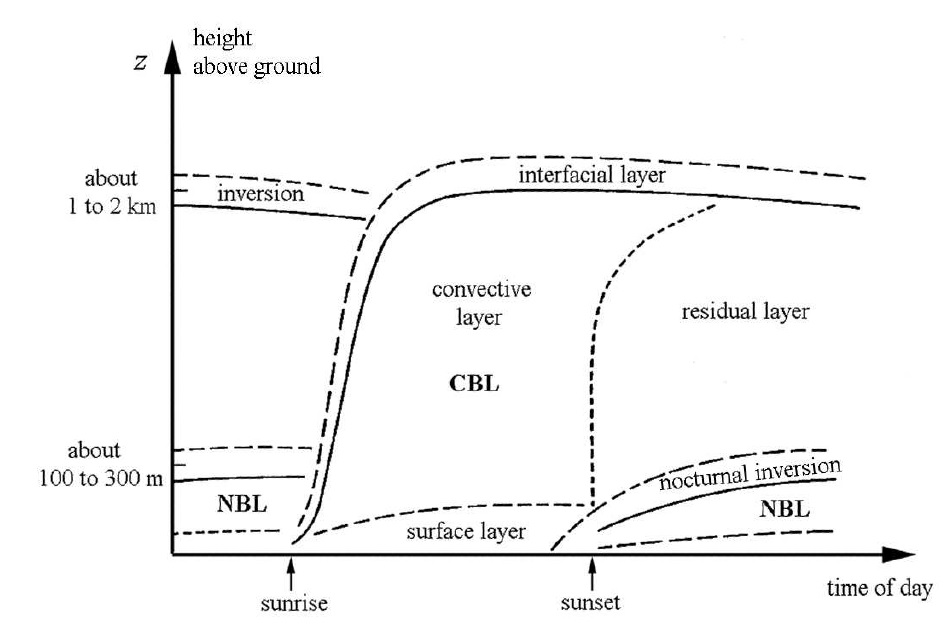
\includegraphics[keepaspectratio, width=0.5\textwidth]{images/chap3/atmospheric_boundary_layer.jpg}
	\caption{Typical evolution of atmospheric boundary layer during the day. Convective boundary layer extension is shown~\cite{bib:li}} 
	\label{fig:atmo_bl}
\end{figure}
To achieve the zero emission, a green source of energy (batteries, in specific case), must be taken into account.  

The top level requirements for this LPA, based on DEP and different energy sources, are reported in Table~\ref{tab:tlar_aircraft_dep}.
They are similar to the Airbus A320 requirements, resized for 2035 and explored in Sec.~\ref{subsubsec:chap2_a320_optim_eis2035}; note that the zero emission requirement appears clearly as a TLAR.  
\begin{table}[!h]
	\centering
	\begin{tabular}{l r l}
		\hline
		Range & 600--1500 & nmi \\
		Mach number & 0.78 & \\
		Number of passengers & 150 & \\
		Approach speed & 132 & kt \\
		EIS & 2035 & \\
		Zero emission limit & 3000 & ft \\
		\hline
	\end{tabular}
	\caption{Top level requirements for the proposed TAW configuration featuring distributed electric propulsion, shown in Fig.~\ref{fig:aircraft_dep_concept}.}
	\label{tab:tlar_aircraft_dep}
\end{table}

A visualisation of the concept to investigate is depicted in Fig.~\ref{fig:aircraft_dep_concept}, using OpenVSP~\cite{bib:openvsp}. 
The hybridization is obtained through a set of batteries, located in the cargo and not shown in Fig.~\ref{fig:aircraft_dep_concept}, and two turboshafts located at the rear.
Because of the rear turboshaft position, a T-tail must be used for the empennage configuration. 
More details on the hybrid chain and its modelisation are provided in next section. 
\begin{figure}[!h]
	\centering
	\includegraphics[keepaspectratio, width=0.7\textwidth]{images/chap3/aircraft_dep_concept.jpg}
	\caption{Classical TAW configuration featuring distributed electric propulsion concept, as modeled in OpenVSP~\cite{bib:openvsp}.}
	\label{fig:aircraft_dep_concept}
\end{figure}
Electric motors and ducted fans are placed over the wing, to take advantage of blowing effect, especially for takeoff and landing phase~\cite{bib:moore_2018, bib:deere_2017b}. 
To maximise this phenomenon, a hyperdistributed configuration is considered, that is more than 15-20 ducted fans are used. 
Beside the blowing effect, this solution is easier to implement, compared to others (\textit{e.g.} embedded engines), and limits the associated risk~\cite{bib:mukhopadhyay_2018}. 
Also, it has been shown in the work of Wick et al.~\cite{bib:wick} that it does not produce wave drag divergence in transonic regime. 

On this configuration, the BLI effects can be neglected because of the small chord available on the wing. 
Therefore, the blowing is the only aero-propulsive effect taken into account. 
From the AMPERE experience at ONERA~\cite{bib:ampere_ref}, such phenomenon produces full laminary flow on the upper surface, increasing the local 2D lift to values in the range of 4-5. 
As a consequence, takeoff length is reduced, the wing area is reduced, and high-lift devices are no more needed, saving weight. 
The blowing, however, may lead to tip-stall problem.
To force the stall starting at the center of the wing, a twist law must be defined~\cite{bib:cdn_notes}. 
The research of an appropiate twist law, however, has not been tackled in this research, which is limited to the development of an OAD procedure for the concept, and it is marked among the further developments. 

The advantages of distributed propulsion in case of failure condition have already been discussed in Chapter~\ref{chap1:state_art} (see also the work of Steiner et al.~\cite{bib:steiner}). 
Its effect on the mass is also been discussed in Sec.~\ref{subsubsec:chap1_dep_review} in the case of DRAGON configuration~\cite{bib:dragon}. 
In particular, it has been remarked that from one hand distributed propulsion alleviates the aerodynamics load, but on the other hand enhances the torsion moment, leading to an increasing in wing weight. 

Concerning the position of batteries, as said they are located in the cargo.
This choice was mainly dictated by stability needings: batteries introduce a non negligeable punctual weight that may strongly affect the center of gravity; placing them in the cargo reduces their impact since the global center of gravity is found around the wing center of gravity. 
Also, the cargo is the zone that offers more volume available for its allocation. 

After this general overlook on the concept, next section details the propulsion system, presenting a general overlook and then the modelisation of each component. 

\section{Definition of an hybrid propulsive chain}
\label{sec:chap3_prop_chain_desc}

The general scheme, in the case of 40 distributed motors, is represented in Fig.~\ref{fig:dep_scheme}.
The number of motors is chosen as it is indicative of a hyperdistributed architecture, which is considered in this work. 
The two turboshafts, referred also as gas turbines, are connected to a device, called generator, that converts mechanical power into electrical power. 
They are coupled to a set of batteries thanks to a set of electrical buses, also called power management units PMU or electric cores. 
From the PMU dedicated lines start, one for each electric motor, aimed to convert electric power in mechanical power. 

The current is brought in DC way, at this scope along the lines there are AC/DC and DC/AC devices to switch the current type from DC to AC and vice versa, and DC/DC devices to bring the current at the right transport voltage. 
Finally, breakers are installed to disconnect a line in case of failure.
\begin{figure}[h!]
	\centering
	\includegraphics[keepaspectratio, width=\textwidth]{images/chap3/dep_scheme}
	\caption{General scheme of hybrid electric distributed propulsive chain architecture considered in this reseach. Case of 40 engines distributed along the wing.}
	\label{fig:dep_scheme}
\end{figure}

It is to note that each power source supplies power to the whole electric buses, to increase redundancy and avoid power losses in case of a core failure. 
Electric motors are directly connected through the shaft to the ducted fan, which finally converts mechanical power into thrust.
From an architecture point of view, the power that arrives at the electric cores is the sum of the battery and the turboshaft power, so they work like in a serial architecture. 
After the cores, instead, power is splitted along all the lines, keeping the voltage constant, and this part of the scheme works as a parallel architecture. 
Therefore, the global arrangement could be defined as a mix-type architecture. 

The propulsive chain is more complex than a traditional one, but it can rely on better efficiency due to the electrification, with potential reduction in fuel consumption. 
Still, because of the complexity and weight penalties, it may require more maintenance, which leads to higher maintenante cost, and thus a deeper analysis has to be carried out~\cite{bib:pornet_cost}. 

Concerning the power management, this research proposes a different approach than the hybrid ratio used in previous work~\cite{bib:pornet, bib:isikveren}. 
One of the limit of the degree of hybridisation is the flexibility: in fact, in case of a sudden loss of power, it is still distributed between the sources at the same percentage, and the power demanded to each source is always dependent on the other. 
Instead, here it has been preferred to control each source separately, with a dedicated power rate defined as following:
\begin{subequations}
	\label{eq:power_rates}
	\begin{equation}
		\label{eq:battery_power_rate}
		\delta_b = \frac{P_b}{P_{b_{\max}}}
	\end{equation}
	\begin{equation}
		\label{eq:tshaft_power_rate}
		\delta_{GT} = \frac{P_{GT}}{P_{GT_{\max}}}
	\end{equation}
\end{subequations}
where $\delta_b$ and $\delta_{GT}$ are the battery and the turboshaft power rate respectively, $P_b$ and $P_{ts}$ the delivered power by battery and turboshaft, and the subscript $\max$ refers to their maximum value (as the turboshaft output depends on Mach and altitude, since it is an air breathing engine). 
The total power arriving at the core level is then
\begin{equation}
	\label{eq:total_power_core}
	P_{c} = \delta_b \eta_b P_{b_{\max}} + \delta_{GT} \eta_g P_{GT_{\max}}
\end{equation}
where $\eta$ represents the efficiency of batteries and generator. 
In this way, power demanded to turboshafts and batteries are decorellated, and the advantage of this approach is in the flexibility that it permits in case of failure.
If a sudden loss of source occurs, in fact, it is still possible to ask for more power to the other source, since the two sources can deliver their maximum power at the same time, whereas before this was not possible since an increase in the degree of hybridisation results in a major power request from one source and less from the other one.

Finally, a remark on the technological choice must be done. 
There are two possible solutions for the upcoming years: a non-cryogenic technology, where the components are further developed but without considering the superconductivity~\cite{bib:dever}, or a cryogenic technology, where the use of superconductivity allows to drastically lighten the system without any heat dissipation~\cite{bib:madavan}.
The cryogenic technology has potentially much more advantages than the non-cryogenic one, however it is still under experimentation and it is unforeseen to have it ready at large power scale before the 2040~\cite{bib:brelje_biblio}.
Therefore, to reduce at most the risk related to the design, a more conventional non-cryogenic technology is here considered, within the 2035 perspectives.

Next sections will present the model implemented for each of the components.
When dealing with electric components, the key parameters are the specific energy and the specific power density; following the notation used by Brelje and Martins~\cite{bib:brelje_biblio}, these quantities are represented as the lower case of extensive quantities ($e$ for specific energy density, $p$ for specific power density).

\subsection{Battery}
\label{subsec:chap3_batt_model}

Battery is a vital component of electric achitecture as it is a main source of power, while corresponding to a permanent weight penalty. 
Beside the power, battery is also an energy source, and generally its overall performance is classified based both on the energy and the power content, through the use of a Ragone plot~\cite{bib:ragone}. 
This curve shows, for a given category of battery, the tradeoff between specific power and the specific energy; sometimes it is referred in equivalent way to volumetric quantities. 
The tradeoff between the two parameters is almost exponentially decreasing: the more powerful a battery is, the less energetic is and viceversa. 
The choice is then not unique but depends on the case of application, \textit{i.e.} for small aircraft the power level is not so relevant and a more energetic battery is of more interest~\cite{bib:hepperle}, on the contrary for larger size aircraft power may become the most stringent criteria to supply~\cite{bib:kim_n3x_2014}. 
An example of Ragone plot, for different types of batteries, is given in Fig.~\ref{fig:battery_classification_ragone}. 
\begin{figure}[!h]
	\centering
	\includegraphics[keepaspectratio, width=0.6\textwidth]{images/chap3/battery_class_ragone.jpg}
	\caption{Ragone plot for different type of batteries, 2008 technology state of the art~\cite{bib:simon}.}
	\label{fig:battery_classification_ragone}
\end{figure}

In recent years, research has been focusing in developing new technologies for the upcoming generation of batteries: beside the classical Lithium ones, other developments are focusing on the studying of Sulphur, Nickel, Polymer based batteries, and even a new innovative category of air-breathing batteries, the so-called Lithium-Air~\cite{bib:fraunhofer, bib:heide}. 
The research in this field, however, still corresponds to the experimentation stage and in some cases even at theoretical level; choosing such innovative aspects in the design is a significant risk. 
On the contrary, the actual Lithium-Ion technology is well assessed, and it cover a large variety of situations, from high power to high energy (see also Fig.~\ref{fig:battery_classification_ragone})~\cite{bib:xue}.
Despite the theoretical limit for these batteries is almost reached~\cite{bib:fraunhofer}, in this research it has been decided to use Li-Ion, in order to reduce the risk related to the design.  

A battery is defined by a set of five parameters: specific energy density $e_b$, specific power density $p_b$, density $\rho_{b}$, energy density and power density~\cite{bib:cinar_methods, bib:lowry}.
Actually, they are not independent of each others, but only three of them are necessary for a full definition. 
The first and most natural input is the phisical density $\rho_{b}$; the two other independent parameters can be equivalently specific energy and power density, or volumetric energy and power density, as from the Ragone plot.
In this work $\rho_{b}$, $e_{b}$ and $p_{b}$ are given as inputs; energy and power density follow to be $\rho_{b} e_{b}$ and $\rho_{b} p_{b}$.
The energy stored $E_{b}$ and the maximum power $P_{b}$ which can be delivered by the battery are then computed:
\begin{equation}
E_{b} = e_{b}m_{b} = e_{b}\rho_{b}\tau_{b}
\label{eq:battery_energy}
\end{equation}
\begin{equation}
P_{b} = p_{b}m_{b} = p_{b}\rho_{b}\tau_{b}
\label{eq:battery_power}
\end{equation}
where $\tau_{b}$ is the battery volume and $m_{b}$ is the battery mass.

Another key aspect of batteries is their dynamic: during the use, their capacity, that is the integral of current over the time, changes together with the voltage delivered.
A typical battery discharge curve, representing voltage vs. capacity, is shown in Fig.~\ref{fig:discarghe_battery}.
Three regions are usually identified: an exponential zone, at low capacity, that in general can be neglected, a region in which the voltage is constant, and finally a region in which voltage drops rapidly (deep discharge zone).
\begin{figure}[!h]
	\centering
	\includegraphics[keepaspectratio, width=0.4\textwidth]{images/chap3/battery_discharge_curve.jpg}
	\caption{Typical battery discharge curve voltage vs capacity; with the three characteristic regions identified~\cite{bib:tremblay}.}
	\label{fig:discarghe_battery}
\end{figure}

To avoid damaging the system, a battery should not work in the deep discharge zone. 
To monitor its state the state of charge \textit{SoC}, defined as the ratio between the capacity at a certain time $q\left(t\right)$ and the total capacity $q_b$, is used:
\begin{equation}
\label{eq:soc_orig}
SoC\left(t\right) = 1 - \frac{q\left(t\right)}{q_{b}}
\end{equation}
where $q\left(t\right)=\int_{0}^{t} i\left(s\right)ds$, with $i\left(s\right)$ the current intensity at time \textit{s} and $q_b=q(t_f)$, with $t_f$ the final time.
To avoid the deep discharge zone, \textit{SoC} can not be allowed under a certain limit, which in general depends on the battery type.
For a Li-Ion battery the minimum limit for the \textit{SoC} is estimated to be 20\%~\cite{bib:lowry, bib:tremblay}.
Finally, the total battery energy, defined in Eq.~\eqref{eq:battery_energy}, is also the area under the discharge curve:
\begin{equation}
\label{eq:battery_energy_int}
E_b = \int_{0}^{V_{f}}q\left(V\right)dV = \int_{0}^{V_{f}} \int_{0}^{t_{f}}i\left(s\right)dsdV.
\end{equation}

At conceptual design level, it is a hard work to implement the full battery dynamic into the model, due to the huge number of variables involved~\cite{bib:tremblay}.
For that reason, in this work the dynamic behaviour is neglected and the hypothesis of constant voltage is made; in other words, it is assumed that the exponential zone can be neglected and the 20\% limit ensures to avoid the deep discharge zone.
Under this hypothesis, it is possible to remove $dV$ from the integral in Eq.~\eqref{eq:battery_energy_int}:
\begin{equation}
\label{eq:battery_energy_simple}
E_b = \Delta V \int_{0}^{t_{f}} i\left(s\right)ds = \Delta V q_b
\end{equation}
Note that in Eq.~\eqref{eq:battery_energy_simple} the quantity $\Delta V$, which is total costant voltage, appears. 
Finally, multiplying by $\Delta V$ both numerator and denominator in Eq.~\eqref{eq:soc_orig}, the \textit{SoC} at time \textit{t} can be written in terms of energy:
\begin{equation}
\label{eq:soc}
SoC\left(t\right) = 1 - \frac{E_{c}\left(t\right)}{E_{b}},
\end{equation}
where $E_{c}\left(t\right)$ represents the energy consumption at time $t$.
The assumptions here are not restrictive and this approach is used in this study.

The other advantage of this model is that defining a battery discharge curve the battery energy is fixed, and then the number of batteries has to be treated as design variable in an optimisation process.
Since it is an integer, this quantity can not be easily included and mixed integer nonlinear programming algorithms have to be considered~\cite{bib:belotti}.
On the contrary, the battery volume, which defines energy and power content through Eq.~\eqref{eq:battery_energy} and Eq.~\eqref{eq:battery_power}, can be used in the equivalent way, with the advantage of being a continuous variable. 
This aspect will be recalled later, during the optimisation problem formulation. 

For what it concerns the sizing, batteries must supply both the energy and the power requirements. 
The volume is then computed in order to satisfy the conditions of Eq.~\eqref{eq:battery_sizing_constraint}, $N_b$ being the number of batteries.
\begin{subequations}
	\label{eq:battery_sizing_constraint}
	\begin{equation}
		\label{eq:battery_energy_constraint}
		SoC\left(t_f\right) \geq 0.20
	\end{equation}
	\begin{equation}
		\label{eq:battery_power_constraint}
		N_b P_b \geq P_{ref}
	\end{equation}
\end{subequations}
Eq.~\eqref{eq:battery_energy_constraint} states that the state of charge at the final time must be at least 0.20, for safety issues, meanwhile Eq.~\eqref{eq:battery_power_constraint} states that the power delivered by all the batteries must be higher than a reference power, specified by the designer, which can be \textit{i.e.} the power at takeoff.
Note that this procedure is similar to the wing sizing in the original FAST, where the wing area needs to satisfy at the same time conditions of Eq.~\eqref{eq:wing_approach_condition} and Eq.~\eqref{eq:wing_fuel_condition}. 

The battery mass is simply computed by the volume information as
\begin{equation}
	\label{eq:battery_mass}
	m_b = \rho_{b} \tau_{b}
\end{equation}

\subsection{Gas turbine and generator}
\label{subsec:chap3_gen_model}

Gas turbine is the other main of power source and it is then one of the most important element to size. 
It is no more than an air breathing engines, with the scope to produce power to deliver at the electric chain; its working is similar to the turboshafts that equipe regional aircraft, like the ATR 72~\cite{bib:roux_eng_data}, with the only difference that mechanical power is not delivered to a propeller but to a device that converts it into electric power, called generator. 

In fact, its design is similar to these type of engines: after the inlet, there is a single compressor, followed by the combustion chamber, where the chemical reactions take place, and two turbines~\cite{bib:mattingly}. 
The first turbine is the high speed one, which is mounted on the same shaft of compressor and moves it.
The second turbine, instead, works at low speed, and it is mounted on a different shaft, where the generator is placed. 
Most of the power generated by the combustion is delivered to the high speed turbine; the remaining represents the useful power, which is of interest to compute performances. 

The gas turbine has been developed using GSP, acronym of Gasturbine Simulation Program: it is a software, developed at NLR, for the performance analysis of engines~\cite{bib:gsp, bib:gsp_website}. 
Its scheme, as modeled in GSP, is shown in Fig.~\ref{fig:tshaft_gsp}; it is possible to detect all the elements described above. 
\begin{figure}[!h]
	\centering
	\includegraphics[keepaspectratio, width=0.6\textwidth]{images/chap3/tshaft_gsp.jpg}
	\caption{Turboshaft model, as in GSP software~\cite{bib:gsp_website}.}
	\label{fig:tshaft_gsp}
\end{figure}

The output of the model are the maps for power $P_{GT}$ and fuel flow $\dot{m}_{f_{GT}}$ as function of Mach and altitude, similar to the outputs from the CERAS and the rubber engine described in Sec.~\ref{subsubsec:chap2_fast_propulsion}. 
For the performance, the specific fuel consumption is replaced by the power specific fuel consumption PSFC, defined in Eq.~\eqref{eq:psfc_def}.
\begin{equation}
	\label{eq:psfc_def}
	\textrm{PSFC} = \frac{\dot{m}_{f_{GT}}}{P_{GT}}
\end{equation}
Units for PSFC are \si{\kilogram\per\kilo\watt\per\hour}, a typical value is in the order of 0.22~\cite{bib:burguburu}. 

Finally, the inlet diameter is computed by knowing the value of mass flow, meanwhile the total length is estimated starting from statistical equations given by Raymer~\cite{bib:raymer}.  
To consider a ``rubberized'' version, a scale factor is considered, defined as
\begin{equation}
	\label{eq:tshaft_scale_factor}
	k_{GT} = \frac{P_{GT_{des}}}{P_{GT_{ref}}}
\end{equation}
where $P_{GT_{des}}$ is the needed design power and $P_{GT_{ref}}$ the reference power of the GSP model; note that the design point must be the same to ensure coherency. 
The power map is rescaled according to this factor. 
No changes are considered for the PSFC, since from Eq.~\eqref{eq:psfc_def} emerges that a change in power automatically impacts the PSFC. 

Burguburu and Basset~\cite{bib:burguburu} give an estimation of the mass of this type of engine, considering a large number of different similar turboshaft; from these it is possible to define a power to mass ratio, so the gas turbine mass results to be
\begin{equation}
	\label{eq:tshaft_mass}
	m_{GT} = \frac{P_{GT_{des}}}{p_{GT}}
\end{equation}
 
Concerning the design point, it depends on the designer choice and it may be the takeoff, the cruise or other points. 
In this research batteries can help the takeoff and the climb phase, but design also an hybrid cruise will result unfeasible. 
As a result, the cruise segment is the main segment where the gas turbine works alone, and it is preferrable to have it designed for these conditions.
Table~\ref{tab:tshaft_design_point} reports the design point for the GSP gas turbine; the altitude is taken in a reasonable flight level.
\begin{table}[!h]
	\centering
	\begin{tabular}{l r l}
		\hline
		Mach number & 0.78 & \\
		Altitude & 35 & kft \\
		$\Delta$ISA & 0 & \si{\celsius} \\
		\hline
	\end{tabular}
	\caption{Design point for the gas turbine modeled in GSP.}
	\label{tab:tshaft_design_point}
\end{table} 

\subsection{Electric motor}

Electric motors are the other main component of the hybrid propulsion, aimed to convert electrical power to mechanical power for the shaft. 
They are very reliable devices and can operate at very high efficiency, that, with a careful design, can reach 95-98\%.
Furthemore, respect to a combustion engine, their performances are not dependent from the altitude~\cite{bib:seitz}, which represents their main andvantage. 
Losses are mainly linked to friction of components and magnetic field, Lowry and Larminie presented a full description of all the losses that occur in an electric motor~\cite{bib:lowry}.
Despite all these features, their use has been limited by power-to-mass ratio, but advances in the last decade enabled to reach higher values, which opened their use in aircraft industry~\cite{bib:campbell}. 

Basically, electric motors can be divided into two classes: AC and DC motors.
The former are lighter than the latters, but require complex power conversion hardware to convert the DC current in AC, suitable for the motors. 
On the other side, DC motors tend to be larger than AC motors with the same specification, and require more maintenance. 
The most common DC motors are based on the permanent magnet technology: their advantage is that they do not require an excitation power source to establish a magnetic field, so they can be used as a motor and generator, but they are heavy and very expensive~\cite{bib:campbell}.
As a conclusion, it seems that AC motors represent the best choice to reduce penalties in weight, despite they need DC/AC converters, that are in fact present in the scheme of Fig.~\ref{fig:dep_scheme}, one for each motor line. 

For the sizing, motors are defined by their specific power; knowing the maximum power demanded their weight results to be:
\begin{equation}
	\label{eq:motor_weight}
	m_{EM} = \frac{P_{EM_{\max}}}{p_{EM}}
\end{equation}

The electric motor must be coupled with the ducted fan, and the rotational speed of both the elements must be matched. 
For this purpose, a gearbox must be added, introducing weight to the system, or a more integrated device like the anular motors can be used~\cite{bib:eichenber}. 
An example of anular motor is shown in Fig.~\ref{fig:anular_motor}: the fan is directly integrated within an anular fairing, and it is moved by the magnetic field generated in the external shroud. 
\begin{figure}[!h]
	\centering
	\includegraphics[keepaspectratio, width=0.4\textwidth]{images/chap3/anular_motor.jpg}
	\caption{Scheme of anular motor, which integrates electric motors and ducted fan~\cite{bib:eichenber}.}
	\label{fig:anular_motor}
\end{figure}

Albeit the difficulty in design and the very low power to mass ratio (in the order of 5~\si{\kilo\watt\per\kilogram} according to the work of Eichenber et al.~\cite{bib:eichenber}), an anular motor removes the problem of coupling, since the fan rotational speed is directly controlled by the magnetic field generated. 
The length of the motor is computed by the ratio between length and fan radius:
\begin{equation}
	\label{eq:motor_length}
	L_{EM} = \left(\frac{L_{EM}}{r_{f}}\right)r_{f}
\end{equation}
$r_{f}$ being the fan radius, the sizing of will be explained later in Sec.~\ref{subsec:chap3_duct_fan_sizing}. 
The ratio $\left(\frac{L_{EM}}{r_{f}}\right)$ is function of FPR solely:
\begin{equation}
	\label{eq:motor_length_radius_ratio}
	\left(\frac{L_{EM}}{r_{f}}\right) = \left\{\begin{array}{l l}
		1.25 + 0.5\left(1.1-\textrm{FPR}\right) & \textrm{FPR}\leq 1.1 \\
		1.75 & \textrm{otherwise}
	\end{array}\right.	
\end{equation}
The total radius includes also the external shell; its thickness is estimated to be 5\% of the fan radius. 

\subsection{Inverters and converters}
\label{subsec:chap3_ic_model}

The DC/AC and AC/DC devices are present along all the lines, to swith from DC current, which is the type that goes in cables, to AC current, needed for the electric motors. 
These devices are commonly called inverters. 
Another type of device is the DC/DC, called converter, that brings a DC current at the right voltage, and it is placed in the battery pack. 

They are simply defined by the power specific density and the efficiency.
Their sizing is similar to that already adopted for the other elements: starting from the knowledge of the maximum power they need to sustain, their mass is computed by the definition of the power specific density, as in Eq.~\eqref{eq:ic_mass}.
\begin{equation}
\label{eq:ic_mass}
m_{IC} = \frac{P_{{IC}_{\max}}}{p_{IC}}
\end{equation}

The value of maximum power depends by the location at which they are placed in the chain of Fig.~\ref{fig:dep_scheme}: the inverters before the motors need to sustain a level of maximum power equal to that of the motors, divided by their efficiency, meanwhile the inverters after the core must sustain a maximum power that is greater because there were some loss due to efficiency and transport. 

\subsection{Power management unit PMU}
\label{subsec:chap3_core_model}

The power management unit (PMU), sometimes referred also as electric core, is the device aimed to electrically connect the gas turbines and the batteries. 
It can be schematised as an electrical node, which takes two lines and spread them to transport power to electric motors. 
In general, more than one of these units are located in the chain for redundancy; also, as shown in Fig.~\ref{fig:dep_scheme}, each power source is connected to all the cores, in order to avoid a power loss in case of core failure. 

They are defined by an efficiency and a power density, similar to other components their mass is estimated as:
\begin{equation}
\label{eq:core_mass}
m_{core} = \frac{P_{{core}_{\max}}}{p_{core}}
\end{equation}

These devices are highly efficient, however it is to note that a loss of one of them is reflected in a set of engines becoming inoperative; the remaining working engines are:
\begin{equation}
	\label{eq:oci_inoperative_neng}
	N_{EM_{op}} = \frac{N_{core}-1}{N_{core}}N_{EM}
\end{equation} 
From Eq.~\eqref{eq:oci_inoperative_neng} it is evident that the more the propulsion is distibuted, that is more core are present, the less is the quantity of engines becoming inoperative. 
That is, a highly distributed propulsion system, at core level, helps to reduce the penalties due to the oversizing, which is the equivalent effect studied by Steiner et al. in relation to the engine failure~\cite{bib:steiner}. 
This aspect, together with the increased propulsive efficiency, is really the key point of interest for distributed propulsion. 

\subsection{Cooling system}
\label{subsec:chap3_cooling_system}

Thermal aspects are of relevant importance in an hybrid architecture.
Generally, electric components show a very high efficiency, with small loss. 
Nevertheless, due to high values of power used, in the order of megawatt, a sizable quantity of this power is dissipated into heat. 

A cooling system must be added, to avoid that the temperature increases beyond the satefy limit, damaing the systems within the propulsive chain or even the airframe. 
Of course, such system introduces a relevant penalty in weight, and thus a careful design must be carried out, to limit penalties. 

A cooling system consists of two different devices: heat exchanger and air cooling systems.
Heat exchanges are devices that surround the cables and artificially dissipate the power using air, meanwhile the latter are air inlets and associated ducting placed in the fuselage, in order to have cold air circulating into the system.
The heat exchanger introduces a mass penalty, that can be evaluated knowing the value of power to dissipate~\cite{bib:anton}:
\begin{equation}
m_{cs} = \frac{P_{diss}}{p_{cs}}
\label{eq:cs_mass}
\end{equation}
with $m_{cs}$ cooling system mass, $P_{diss}$ power dissipated and $p_{cs}$ cooling system specific power.
Air cooling does not introduce weight but incurs a penalty on the drag coefficient, estimated to be 5\% with the equations presented by Hoerner~\cite{bib:hoerner}.

\subsection{Cables}
\label{subsec:chap3_cable_model}

The cables have to transport current from one device to another within the hybrid architecture. 
They are sized in order to carry a certain current, which must be below the maximum allowed threshold~\cite{bib:vanbogaert}.
The current, and so the sizing, depends on the voltage used for the transport. 

First the current which flows through a cable is computed as
\begin{equation}
i = \frac{P}{\Delta V}
\end{equation}
Then a check has to be done in order to be sure that value is lower than the maximum current. 
If it is not, more cables have to be installed; the number is computed dividing the value of current with the maximum one:
\begin{equation}
N_{cab} = \left[\frac{i}{i_{max}}\right]
\end{equation} 
where the square brackets indicate the integer part of $\frac{i}{i_{max}}$. 
The number of cables is then doubled to consider that current can move in both directions. 
Finally, according to motors, generators and batteries positions, it is possible to estimate the cable length and so the weight:
\begin{equation}
m_{cab} = N_{cab}\left(\frac{m}{L}\right)L_{cab}
\end{equation}
where $\frac{m}{L}$ is the cable linear density. 
Installation and Healt Monitoring System have to be included in the weight calculation: preliminary works at ONERA show an increasing in weight of 30\% for the installation and of 5\% for the HMS.

During the transport, a certain amount of power that is dissipated into heat due to the Joule effect~\cite{bib:tipler}; these losses can be evaluated using the Ohm's second law: 
\begin{equation}
	\label{eq:2nd_ohm_law}
	P_{cab_{diss}} = R_{cab} i^2
\end{equation}
where $R_c$ is the resistance, computed with the classical equation
\begin{equation}
	\label{eq:resistance}
	R_{cab} = \rho_{cab} \frac{L_{cab}}{S_{cab}}
\end{equation}
where $\rho_{cab}$ is the electrical resistivity and $S_{cab}$ the cable section area. 
For copper, $\rho_{cab}=1.68\times10^{-8}$~\si{\ohm\meter} at 20~\si{\celsius}. 
The power dissipated is subtracted from the total useful power and added to the power sizing for cooling system.

A cable efficiency can be defined considering the total electric power $\Delta V i$ and the power loss of Eq.~\eqref{eq:2nd_ohm_law}:
\begin{equation}
	\label{eq:cable_efficiency}
	\eta_{cab} = \frac{\Delta V i - R_{cab}i^2}{\Delta V i} = \frac{\Delta V - R_{cab}i}{\Delta V}
\end{equation}
To note that the power loss is equivalent to the loss of tension, in agreement with the 1st Ohm's law~\cite{bib:tipler}. 

\subsection{Ducted fan}
\label{subsec:chap3_duct_fan_sizing}

Ducted fan is the ending point of the propulsive chain, and it is deputed to generate thrust, starting from the mechanical power received by the shaft. 
It is sized to be adapted for a single point, which is typically the cruise point, corresponding to a certain altitude $h$ and Mach number $M_0$. 
Since it is none more than a duct with air passing through, it can be schematised as a nozzle where quasi-isoentropic transformation takes place: under this assumption, it is possible to get a sizing using thermodynamic isentropic equations~\cite{bib:fermi, bib:carlomagno, bib:landau}.
The model described here has been provided by m. Olivier Atinault, research engineer at ONERA Meudon, and published in the AIAA SciTech proceedings~\cite{bib:sgueglia}.

The scheme of the fan with all the sections detailed is shown in Fig.~\ref{fig:ducted_fan_scheme}; the description that follows refers to this scheme. 
The main parameter that drives the design is the fan pressure ratio FPR, which represents the pressure gauge at the fan section. 
As remarked in Sec.~\ref{subsubsec:chap1_dep_review}, FPR impacts both the size and the thrust generated: the smaller, bigger is the size and lower the thrust, and viceversa. 
\begin{figure}[h]
	\centering
	\includegraphics[keepaspectratio, width=0.65\textwidth]{images/chap3/ducted_fan_scheme.jpg}
	\caption{Scheme of a ducted fan for the model presented} 
	\label{fig:ducted_fan_scheme}
\end{figure}
The sizing starts from the thrust coefficient, defined as
\begin{equation}
	\label{eq:thrust_coeff}
	c_T = \frac{T}{\frac{\gamma_a}{2}p_{s_{0}}M_{0}^2S_{ref}}
\end{equation}	
where $T$ is the thrust, $p_{s_{0}}$ is the static pressure at the given altitude, $\gamma_a$ the ratio between the volume coefficients for air, $\gamma_a=1.4$~\cite{bib:fermi}, and $S_{ref}$ an arbitrary reference surface. 

The steps to follow are listed below.
\begin{enumerate}
	\item The first step is to compute the total pressure and temperature at the inlet, using the de Saint-Venant relations~\cite{bib:carlomagno}:
	\begin{equation}
		\label{eq:total_pressure_pt0}
		p_{t_{0}} = p_{s_{0}}\left(1+\frac{\gamma_a-1}{\gamma_a}M_0^2\right)^{\frac{\gamma_a}{\gamma_a-1}}
	\end{equation}
	\begin{equation}
		\label{eq:total_temperature_tt0}
		\theta_{t_{0}} = \theta_{s_{0}}\left(1+\frac{\gamma_a-1}{\gamma_a}M_0^2\right)
	\end{equation}
	
	with $\theta_{s_{0}}$ representing the static temperature at the given altitude. 
	
	\item Then it is possible to compute the Mach number at the exit of the nozzle:
	\begin{equation}
		\label{eq:mach_nozzle_m3f}
		M_{3_{f}} = \sqrt{\frac{2}{\gamma_a-1}\left[\left(1+\frac{\gamma_a-1}{\gamma_a}M_0^2\right)\mathrm{FPR}^{\frac{\gamma_a-1}{\gamma_a}}-1\right]} = f(M_0,\mathrm{FPR})
	\end{equation}
	This relation is obtained considering the nozzle is adapted, that is the pressure at the exit is equal to the ambient pressure ($p_{3_{f}}=p_{s_{0}}$). 
	It is also possible to compute the velocity ratio $\beta$ as follows:
	\begin{equation}
	\label{eq:velocity_ratio_beta}
		\beta=\frac{V_{3_{f}}}{V_0}=\frac{M_{3_{f}}}{M_0}\sqrt{\frac{\theta_{3_{f}}}{\theta_0}}=\frac{M_{3_{f}}}{M_0}\sqrt{\mathrm{FPR}^{\frac{\gamma_a-1}{\eta_f\gamma_a}}\frac{1+\frac{\gamma_a-1}{2}M_0^2}{1+\frac{\gamma_a-1}{2}M_{3_{f}}^2}}=f(M_0,\mathrm{FPR})
	\end{equation}
	$\eta_f$ being the polytropic efficiency of the fan. 
	If $\eta_f$=1 the compression is isentropic. 
	In practice it is possible to compute the polytropic efficiency with the semiempirical relation: 
	\begin{equation}
		\label{eq:fan_eff_etaf}
		\eta_f=\num{0.98}-\num{0.08}\left(\mathrm{FPR}-1\right)
	\end{equation} 
	
	\item At this stage it is possible to compute the nozzle exit area:
	\begin{equation}
		\label{eq:s3f_ratio_fan}
		\frac{S_{3_{f}}}{S_{ref}}=\frac{c_T}{2}\mathrm{FPR}^{\frac{\gamma_a(1-\eta_f)-1}{\gamma_a\eta_f}}\left(\frac{1+\frac{\gamma_a-1}{2}M_0^2}{1+\frac{\gamma_a-1}{2}M_{3_{f}}^2}\right)^{\frac{1}{\gamma_a-1}}\frac{1}{\beta^2-\beta}=f(M_0,\mathrm{FPR},c_T)
	\end{equation}
	Finally, supposing the section circular, it is possible to deduce the exit diameter:
	\begin{equation}
		\label{eq:fan_exit_diameter}
		D_{3_{f}} = 2\sqrt{\frac{A_{3_{f}}}{\pi}}
	\end{equation}
	
	\item At this step it is possible to compute the mass flow and then the power required by the fan. 
	The required mass flow which enters the fan is:
	\begin{equation}
		\label{eq:mass_flow_fan}
		\dot{m}=p_{3_{f}}M_{3_{f}}S_{3_{f}}\sqrt{\frac{\gamma_a}{R\theta_{3_{f}}}}=p_{3_{f}}M_{3_{f}}S_{3_{f}}\sqrt{\frac{\gamma_a}{R\theta_{t_{3_{f}}}}}\left(1+\frac{\gamma_a-1}{2}M_{3_{f}}^2\right)^{\frac{1+\gamma_a}{2(1-\gamma_a)}}
	\end{equation}
	with $p_{t_{3_{f}}}=p_{t_{0}}\mathrm{FPR}$ from the fan pressure ratio definition and $T_{t_{3_{f}}}=T_{t_{0}}\mathrm{FPR}^{\frac{\gamma_a-1}{\gamma_a\eta_f}}$. \\
	
	The total enthalpy variation is then
	\begin{equation}
		\label{eq:delta_h_fan}
		\Delta h = c_p(\theta_{t_{3_{f}}}-\theta_{t_{0}})=\frac{\gamma_a R}{\gamma_a - 1}\theta_{t_{0}}\left(FPR^{\frac{\gamma_a-1}{\gamma_a\eta_f}}-1\right)
	\end{equation}
	and finally the power required by the fan is 
	\begin{equation}
		\label{eq:power_fan_req}
		P_{f}=\Delta h\dot{m}
	\end{equation}	
	
	\item It is finally possible to compute the fan area. 
	For aerodynamics reasons, the Mach number at the fan section is fixed to a maximum value of 0.65 ($M_f=0.65$); the fan area results to be
	\begin{equation}
		\label{eq:fan_area}
		S_{f} = \frac{\dot{m}}{p_{t_{0}}M_{f}\sqrt{\frac{\gamma_a}{R\theta_{t_{0}}}}\left(1+\frac{\gamma_a-1}{2}M_{f}^2\right)^{\frac{1+\gamma_a}{2(1-\gamma_a)}}}
	\end{equation}
	Fan radius is obtained from the ratio between the tip and the hub radius $\sigma$:
	\begin{equation}
		\label{eq:fan_radius}
		r_{f}=\sqrt{\frac{S_{f}}{\pi(1-\sigma_f^2)}}		
	\end{equation}
	
\end{enumerate}

The parameter $\sigma_f$ depends on the technological level: at today, reasonable value based on commercial engines is between 25-30\%~\cite{bib:roux_eng_data}.

Note from Eq.~\eqref{eq:fan_eff_etaf} that the fan efficiency solely depends on the FPR: the lower, the more efficient is the fan, in agreement with what has been explained earlier concerning the power required.
For high values of FPR the power demander to achieve a given $c_T$ increases; on the other hand, the fan size decreases, with a consequent improvement of the aerodynamics due to lower wetted surface.
The tradeoff between size and power as function of FPR is shown in Fig.~\ref{fig:rfan_preq_comp}, for $c_T=9.86\times10{-2}$, $M_0=0.78$ and $h$=35000~ft. 
\begin{figure}[!h]
	\centering
	\includegraphics[keepaspectratio, width=0.6\textwidth]{images/chap3/fan_param_tradeoff}
	\caption{Fan radius (in blue) and required power (dashed line) as function of FPR, $c_T=9.86\times10^{-2}$, $M_0=0.78$ and $h$=35000~ft.}
	\label{fig:rfan_preq_comp}
\end{figure}

Another interpretation of $\eta_f$ can be given introducing the ratio between total pressure and total temperature through the fan: 
\begin{equation}
	\label{eq:total_temp_ratio}
	\frac{\theta_{t_{3_{f}}}}{\theta_{t_{0}}}=\left(\frac{p_{t_{3_{f}}}}{p_{t_{0}}}\right)^{\frac{\gamma_a-1}{\gamma_a \eta_f}}
\end{equation}
Eq.~\ref{eq:total_temp_ratio} shows that at the fan section there is a loss of total quantities related to the polytropic tranformation, which becomes more and more relevant when $\eta_f$ decreases.
Of course, if total quantities are lower, the energy produced is smaller and then the power required needs to be higher to keep $c_T$ constant.

The fan size can not prescind by local flow: the velocity at tip blade must never exceed a certain value, for aerodynamics consideration. 
The maximum allowable speed at the tip is not constant but depends also on the FPR; Fig.~\ref{fig:vtip_design_space} shows the feasible design domain for this variable, indicated as $V_{tip}$. 
In case the point lies in the shaded region, which is a non feasible domain, FPR, $\sigma_f$ are the variables on which it is possible to act to have proper design. 
\begin{figure}[!h]
	\centering
	\includegraphics[keepaspectratio, width=0.6\textwidth]{images/chap3/vtip_design_space}
	\caption{Allowable region for the velocity at the tip of fan blade. The shaded region represents a non feasible space.}
	\label{fig:vtip_design_space}
\end{figure}

Finally, other two relevant parameters are the rotational speed $\Omega$ and the torque $\Theta$, that can be computed as follow:

\begin{subequations}
	\label{eq:fan_perfo}
	\begin{equation}
		\label{eq:fan_rpm}
		\Omega_{f} = \frac{V_{tip}}{r_{f}}\frac{60}{2\pi}
	\end{equation}
	\begin{equation}
		\label{eq:fan_torque}
		\Theta_{f} = \frac{P_{f}}{\Omega_{f}\frac{2\pi}{60}}
	\end{equation}
\end{subequations}
The units are round per minute for the rotational speed and \si{\newton\second} for the torque. 
  
The process just described has an estimated error of less than 10\% on the power demanded. 
As a design point, the first cruise point is the best choice: generally the cruise is the longest segment, and thus it is good practice to have the fan adapted for that condition; the first point is also the point in which aircraft is heavier, and then it is the most stringent. 
In case of off design conditions, a different value of FPR which provides the same $S_{3_{f}}$ has to be found.
In practice, FPR variation corresponds to a different rotational speed on a real fixed-pitch fan. 

\subsection{Certification constraint module}
\label{subsec:chap3_ccm_hybrid}

A discussion about a new propulsive system can not avoid an overview of failure cases. 
Albeit the CS-25 do not include yet any rule regarding hybrid/electric aircraft, some assumptions need to be made, at least to justify the design choices and reduce risks related to the concept. 

The starting point are again the CS-25~\cite{bib:cs25} and the CATPOL~\cite{bib:catpol} certification, summed up in Table~\ref{tab:ccm_rules}. 
The CAT.POL.410(a)-1 and 2, as well as the CS-25.119(a) and CS-25.121(d) consider the All Engine Operative condition, and thus can be retained as they are. 
Issue arises with the others, where the One Engine Inoperative condition must be replaced by something different. 
In particular, in an hybrid architecture there are two possible scenario to consider:
\begin{enumerate}
	\item Core failure, which corresponds to a certain number of engines inoperative. 
	This condition, however, does not impact the total amount of power delivered, which is still the same. 
	
	\item One power source failure, which corresponds to a loss of total power available and, as a consequence, of thrust.
\end{enumerate}
In the first case, there is no loss of power, but this power must be redistributed among the remaining motors working, computed from Eq.~\eqref{eq:oci_inoperative_neng}. 
So this condition, that from now on is indicated with the acronym of OCI (One Core Inoperative), defines the maximum level of power that all the components must supply in case of core failure, and it is then the sizing condition for the components, starting from the core up to electric motors.

On the contrary, the second condition corresponds to a loss of power, that is a loss of thrust available, and since the aircraft must comply with the certification the power sources must be oversized, to satisfy the certification constraint. 
So this condition is the sizing one for the components before the electric bus. 

However, it is to note that a simultaneous failure of a gas turbine and a battery is an extremely rare case because of the high efficiency of these elements; also thanks to the power management adopted, see Eq.~\eqref{eq:total_power_core}, there is a certain margin of safety in case of one power source failure, since the other one can be used. 
Then, in this research the OEI condition from Table~\ref{tab:ccm_rules} is simply replaced by a OCI, to properly find the required level of power for the electric components. 
This is not valid for all the hybrid configuration, but only for double source power; in case hybridization is obtained by fuel cell or gas turbine, both the failure conditions must be considered. 

From previous studies, it emerges that among the three rules that consider a failure, the most critic is the CS-25.121(b): indeed, at the end of takeoff aircraft can still benefits from the maximum blowing effect, meanwhile at 400~ft, in climb setting, the effect is much lower. 
Then, the condition of core failure at 400~ft is retained as sizing condition for the electric chain. 

From Eq.~\eqref{eq:non_balanced_flight} it is possible to estimate the minimum thrust needed for each fan to maintain the 2.4\% of slope ($100\tan\gamma_{400} = 2.4$) as
\begin{equation}
	\label{eq:thrust_400}
	T_{400} = m_{400}g\left[0.024 + \frac{1}{\left(\frac{L}{D}\right)}\right]\frac{N_{core}}{N_{core}-1}N_{EM}
\end{equation}
where $m_{400}$ represents the aircraft mass at 400~ft, in the condition of interest.
Corresponding power to generate required thrust $P_{400}$ is obtained from the fan model.
The maximum powers to use in the sizing of electric components are then:
\begin{subequations}
	\label{eq:max_power_elec_comp}
	\begin{equation}
		\label{eq:max_power_em}
		P_{EM_{\max}} = \frac{P_{400}}{\eta_{EM}}
	\end{equation}
	
	\begin{equation}
		\label{eq:max_power_ic}
		P_{IC_{\max}} = \frac{P_{400}}{\eta_{EM}\eta_{IC}\eta_{IC}}
	\end{equation}	
	
	\begin{equation}
		\label{eq:max_power_core}
		P_{core_{\max}} = \frac{P_{400}}{\eta_{EM}\eta_{IC}\eta_{IC}\eta_{core}}
	\end{equation}
\end{subequations}

Finally, since at 400~ft the aircraft must fly fully electric, $P_{400}$ defines also the reference power to use in the battery constraint of Eq.~\eqref{eq:battery_power_constraint}:
\begin{equation}
	\label{eq:battery_power_ref_400}
	P_{b_{ref}} = \frac{P_{core_{\max}}}{\eta_{core}\eta_{IC}\eta_b}
\end{equation}

This last remark concludes the overview on the hybrid chain; next section describes first the new MDA tailored for the proposed concept, based on the models just described, and then the resulting MDO formulation. 

\section{Methodology for the sizing of hybrid aircraft}
\label{sec:chap3_sizing_hybrid}

\subsection{MDA sizing loop}
\label{subsec:chap3_mda_hybrid}

The resulting MDA loop for the hybrid electric aircraft here considered is shown in Fig.~\ref{fig:fast_dep_xdsm}, with the detailed algorithm reported in Alg.~\ref{alg:fast_dep}. 
\begin{figure}[!h]
	\centering
	\includegraphics[keepaspectratio, width=1.3\textwidth, angle=90]{images/chap3/FAST_DEP}
	\caption{FAST xDSM scheme for the version tailored to hybrid aircraft featuring distributed electric propulsion, shown in Fig.~\ref{fig:aircraft_dep_concept}. }
	\label{fig:fast_dep_xdsm}
\end{figure}
\begin{algorithm}[!h]
	\caption{FAST algorithm for the sizing of hybrid aircraft featuring distributed electric propulsion; numbering is referred to xDSM of Fig.~\ref{fig:fast_dep_xdsm}}
	\label{alg:fast_dep}
	\begin{algorithmic}
		\REQUIRE TLAR
		\ENSURE Sized aircraft, drag polars, masses, design mission trajectory
		\STATE 0: Initialise the OAD parameters, according to rules contained in Airbus and ISAE handbook~\cite{bib:airbus_notes}.
		\REPEAT
		\STATE 1: Initialise the loop.  
		\STATE 2: Size the battery, according to Eq.~\eqref{eq:battery_energy_constraint} and Eq.~\eqref{eq:battery_power_constraint}.
		\STATE 3: Compute the wing surface, in order to respect Eq.~\eqref{eq:wing_approach_condition} and Eq.~\eqref{eq:wing_fuel_condition}.
		\STATE 4: Compute initial geometry.
		\STATE 5: Resize the geometry, to match stability constraints.
		\STATE 6: aerodynamics calculation.
		\STATE 7: Mass breakdown calculation. The standard AR 2001/D~\cite{bib:mass_breakdown} is modified to include electric components. 
		\STATE 8: Trajectory analysis. 
		At the end, together with the fuel consumption, this analysis gives in output also the total energy consumption and the final battery SoC. 
		\STATE 9: Update the MTOW.
		\STATE 10: Check if the convergence criteria is satisfied; if not, proceed to next iteration. 
		Beside the criteria on OWE of Eq.~\eqref{eq:fast_conv_crit}, the condition on the state of charge described by Eq.~\eqref{eq:battery_energy_constraint} is added to ensure convergence. 
		\UNTIL {$10 \rightarrow 1$: MDA has converged}   
	\end{algorithmic}
\end{algorithm}
The impact of hybrid architecture on the overall loop is small: the main difference with respect to the diagram of Fig.~\ref{fig:fast_basic} lies in in step 2, where a new analysis is added to size the battery with respect to power and energy requirements, as described by Eq.~\eqref{eq:battery_energy_constraint} and Eq.~\eqref{eq:battery_power_constraint}. 
Similarly to wing area, it gets two values of battery volume, each one satisfying the two equality requirements, and then it takes the maximum between the two. 
At first step, where no informations on the energy consumption are known, the battery volume is initialised with respect to the reference power in the initiator analysis.   

Going deeper into the analysis, the major impacts of hybrid propulsion are in step 4 to 8. 
The geometry calculation needs to considers the new elements of the hybrid chain: the wetted surface is greater because of the nacelle used to contain the engines on the upper wing and the gasturbine nacelles at the rear. 
The last contribution is easily computed by knowing the overall gasturbine dimensions: 
\begin{equation}
	\label{eq:gt_wet_area}
	S_{{GT}_{wet}} = N_{GT}2\pi\left(r_{GT}L_{GT} + 1.05r_{GT} L_{GT}\right)
\end{equation}
The first term of Eq.~\eqref{eq:gt_wet_area} represents the internal wetted surface, meanwhile the second one is the external one. 
The fairing thickness is assumed to be 5\% of the gasturbine radius, in agreement with data on existing engines~\cite{bib:roux_eng_data}.

For the engines nacelle wetted surface the estimation is similar, a scheme of the contributions is given in Fig.~\ref{fig:fan_wet_surf}.
\begin{figure}[!h]
	\centering
	\includegraphics[keepaspectratio, width=0.6\textwidth]{images/chap3/fan_wet_area.jpg}
	\caption{Scheme of ducted fan for the wetted surface estimation}
	\label{fig:fan_wet_surf}
\end{figure}
Nacelle internal surface only accounts in the wetted surface calculations, being the external surface contribution already included in the wing wetted area estimation, as visible in Fig.~\ref{fig:wing_blowing_visualisation}. 
Hub and engine lateral surface must be included, adding a relevant penalty. 
Motors' contribution is then:
\begin{equation}
	\label{eq:nac_wet_area}
	S_{{EM}_{wet}} = N_{EM} 2 \pi \left[r_fL_{EM} + r_{h}L_{EM}\right]
\end{equation}
In Eq.~\eqref{eq:nac_wet_area} $r_h$ represents the hub radius, equals to $\sigma_f r_f$ from the definition of $\sigma_f$, and the motor length $L_{EM}$ is computed with Eq.~\eqref{eq:motor_length} considering an anular motor. 
Another relevant aspect in the geometry module is the components' positioning, since they introduce point masses within the airframe, shifting the center of gravity. 
Table~\ref{tab:elec_comp_cg} reports the location of each electric component in the propulsive scheme considered. 
\begin{table}[!h]
	\centering
	\begin{tabular}{c c}
		\hline
		\textbf{Component} & \textbf{CG location} \\
		\hline
		Electric motors & Over the wing, trailing edge \\
		Gasturbines and generators & Approximately 93\% of the fuselage length \\
		Batteries & Splitted in the front and rear cargo \\
		Inverters and converters & In correspondance of the EMs, generators and batteries \\
		Cooling system & In correspondance of the EMs, generators and batteries \\
		Cables & Estimated by their mass distribution in the airframe \\		
		\hline
	\end{tabular}
	\caption{Center of gravity location of the different electric components, belonging to the propulsive system shown in Fig.~\ref{fig:dep_scheme}.}
	\label{tab:elec_comp_cg}
\end{table}

The high speed aerodynamics analysis (step 6) is slightly modified: since the $C_D$ curve is estimated from the wetted surfaces information, in agreement with Eq.~\eqref{eq:cd0}, a proper estimation of wetted surface at step 4 and 5 is the only thing needed to properly estimate the impact on aerodynamics. 
At low speed, the procedure to get the maximum lift coefficient changes, to consider the blowing effect.
This phenomenon is relevant only in the region where engines are mounted: referring to Fig.~\ref{fig:wing_blowing_visualisation}, the region interested by blowing is the red one. 
\begin{figure}[!h]
	\centering
	\includegraphics[keepaspectratio, width=0.5\textwidth]{images/chap3/blowing_surface.jpg}
	\caption{Blowing surface visualisation: the region interested is indicated by the red colour.}
	\label{fig:wing_blowing_visualisation}
\end{figure} 
The global maximum lift coefficient can be computed as
\begin{equation}
\label{eq:cl_max_blowing}
C_{L_{\max}} = C_{l_{\max}} \frac{S_{blow}}{S_{w}}\cos\Lambda_{25_{w}}
\end{equation}
where $C_{l_{\max}}$ is the maximum local lift coefficient with blowing, $S_{blow}$ the portion of surface interested by blowing and $S_{w}$ the wing surface, and the factor $\cos\Lambda_{25_{w}}$ accounts for three-dimensionality effect introduced by sweep~\cite{bib:abbott}. 
Eq.~\eqref{eq:cl_max_blowing} indicates that to maximize the blowing effect, the ratio of blown surface over total surface as to be as close as possible to 1, that is the reason why in the NASA X-57 distributed propellers cover all the wingspan~\cite{bib:borer_sceptor}. 

The mass breakdown module substantially remains the same, except for the fact that section B is enriched of new elements, to include electric components mass, computed as explained in the previous section. 
The addendum with new elements is described in Table~\ref{tab:hybrid_addendum_mass_breakdown}. 
\begin{table}[!h]
	\centering
	\begin{tabular}{l l}
		\hline
		\textbf{B} & \textbf{Propulsion} \\
		B4 & Cables \\
		B5 & Batteries \\
		B6 & Gasturbine and generators \\
		B7 & Inverters and converters \\
		B8 & Cooling system \\
		B9 & PMU \\		
		\hline
	\end{tabular}
	\caption{Proposed addendum to mass breakdown standard~\cite{bib:mass_breakdown} to include electric components mass.}
	\label{tab:hybrid_addendum_mass_breakdown}
\end{table} 

Finally, performance module is modified to include the presence of two power sources. 
At each iteration $i$ the engine model gives in output the battery and gasturbine power $P_{b_{i}}$ and $P_{GT_{i}}$ (in non balanced flight) or the equivalent power rates $\delta_{b_{i}}$ and $\delta_{GT_{i}}$ (in balanced flight) together with the PSFC.
The energy and the fuel consumption are updated:
\begin{subequations}
	\label{eq:energy_fuel_hybrid_ip1}
	\begin{equation}
		\label{eq:energy_ip1}
		E_{c_{i+1}} = E_{c_{i}} + P_{b_{i}}\Delta t
	\end{equation}
	\begin{equation}
		\label{eq:fuel_hybrid_ip1}
		m_{f_{i+1}} = m_{f_{i}} + P_{GT_{i}}\left(\textrm{PSFC}\right)\Delta t
	\end{equation}	
\end{subequations} 
With the information of energy and fuel consumption during the time step $\Delta t$ it is possible to update the values of aircraft mass and battery SoC:
\begin{subequations}
	\label{eq:state_vector_hybrid_ip1}
	\begin{equation}
		\label{eq:battery_soc_ip1}
		SoC_{i+1} = 1 - \frac{\sum_{j=0}^{i}E_{c_{j}}}{E_b} = SoC_{i} - \frac{E_{c_i}}{E_b} 
	\end{equation}
	\begin{equation}
		\label{eq:ac_mass_ip1}
		m_{i+1} = m_{TO} - \sum_{j=0}^{i}m_{f_{i}} = m_{i} - m_{f_{i}}
	\end{equation}
\end{subequations}
Note that Eq.~\eqref{eq:battery_soc_ip1} is the discrete version of Eq.~\eqref{eq:soc}. 

At takeoff, no rotation is considered anymore~\cite{bib:phillips, bib:anderson_perfo}, thanks to the blowing that provide enough lift to takeoff in gliding, as \textit{i.e.} the B-52 does\footnote{B-52 RAF takeoff video, \url{https://www.youtube.com/watch?v=CCfJmuk-des}}.
As further development, this assumption will have to be checked in detailed aerodynamic studies. 

At this point, the MDA to size the proposed concept is ready, the following step is to integrate it within OpenMDAO to obtain the MDO formulation. 

\subsection{MDO formulation}
\label{subsec:chap3_mdo_hybrid}

In practice, the MDO formulation for the hybrid DEP aircraft is obtained by replacing the MDA of Fig.~\ref{fig:fast_openmdao_basic} with the MDA shown in Fig.~\ref{fig:fast_dep_xdsm}. 
The architecture is still the MDF, with all the advantages and drawbacks already mentioned in Chapter~\ref{chap2:fast_base_mdo}. 
The resulting xDSM diagram is shown in Fig.~\ref{fig:fast_openmdao_dep}, with the procedure details explained in Algorithm~\ref{alg:fast_openmdao_dep}.
\begin{figure}[!h]
	\centering
	\includegraphics[keepaspectratio, width=1.3\textwidth, angle=90]{images/chap3/FAST_OpenMDAO_DEP}
	\caption{xDSM diagram for the integrated version of FAST, tailored to optimisation of hybrid aircraft with distributed electric propulsion.}
	\label{fig:fast_openmdao_dep}
\end{figure}
\begin{algorithm}[!h]
	\caption{Integrated version of FAST algorithm description. Numbering refers to Fig.~\ref{fig:fast_openmdao_dep}.}
	\label{alg:fast_openmdao_dep}
	\begin{algorithmic}
		\REQUIRE Initial design parameters (TLAR), design variables initial vector $\underline{x}^{(0)}$
		\ENSURE Sized aircraft, drag polars, masses, performance, $\underline{x}^*$
		\STATE 0: Initialise the optimisation loop: initial values are read from the xml file.
		\REPEAT
		\STATE 1: Initialise DEP electric components. 
		\STATE 2: Initialise the MDA, used to get a viable aircraft.
		\REPEAT
		\STATE 3: Compute the MTOW.
		\STATE 4: Compute the aircraft geometry and perform the mass breakdown, to estimate weight of all components.
		\STATE 5: Compute the static margin.
		\STATE 6: Aerodynamics calculation, based on the same equations of the original version.
		\STATE 7: Compute the aircraft performance.
		\STATE 8: Check the convergence. 
		Criteria is the same of Eq.~\eqref{eq:fast_conv_crit}.
		\UNTIL {$8 \rightarrow 3$: MDA has converged}
		\STATE 9: Evaluate the objective function.
		 If a gradient based solver is used, this analysis computes also derivatives.
		\STATE 10: Evaluate the design constraints.
		If a gradient based solver is used, this analysis computes also the derivatives of each constraint.
		\STATE 11: Check if the optimisation has converged. If not, this analysis updates $\underline{x}$ for the next iteration.
		\UNTIL {$11 \rightarrow 1$: MDO has converged}
	\end{algorithmic}
\end{algorithm}

Similarly to what has been done with the traditional aircraft, some sizing conditions have become design constraints of the problem. 
In particular, the battery volume $\tau_{b}$ is a design variable, subject to the two constraints of Eq.~\eqref{eq:battery_energy_constraint} and Eq.~\eqref{eq:battery_power_constraint}; again, the two inequalities enlarge the design space exploration, and it is up to the optimiser to find the best value of battery volume that minimises the objective function. 

Also Eq.~\eqref{eq:thrust_400} is rewritten in the following form:
\begin{equation}
	\label{eq:gamma_400_constraint}
	\tan\gamma_{400} \backsimeq \gamma_{400} = \frac{T_{400}}{m_{400}g}\frac{N_{core}}{N_{core}-1}N_{EM} - \frac{1}{\left(\frac{L}{D}\right)} \geq \frac{2.4}{100}
\end{equation}
with $T_{400}=f\left(P_{400}\right)$, and $P_{400}$ is added to design variables vector. 
This equation replaces the old one in the CCM, regarding the CS-25.121(b) condition.
Others certification specifications are treated in a similar manner. 

Note that the variable $P_{400}$ affects the battery design too, through Eq.~\eqref{eq:battery_power_ref_400}. 

\section{Exploration of hybrid aircraft with distributed electric propulsion}
\label{sec:chap3_hybrid_ac_exploration}

\subsection{2035 technology assessment}
\label{subsec:chap3_2035_techno_assess}

One of the main challenges in the design of a hybrid aicraft EIS2035 is to assess the technological caracteristics of electric component at that horizon. 
Indeed, literature review reveals that the perspectives of available technologies in 2035 present large dispersion. 
As an example, for what concerns batteries, Hepperle~\cite{bib:hepperle} proposes a value of $e_b$ equals to 350~\si{\watt\hour\per\kilogram}, whereas Bradley~\cite{bib:bradley_sugar_p2} recommends a value of 750~\si{\watt\hour\per\kilogram}.
Several authors deal with the problem of defining perspectives~\cite{bib:fraunhofer, bib:steiner, bib:bradley_sugar_p2_v2, bib:hepperle, bib:dever, bib:brown_n3x, bib:kuhn, bib:naec, bib:madavan, bib:cinar_methods, bib:pornet_2014} for the key technological parameters, notely the power density and the efficiency; Table~\ref{tab:techno_design_space} reports the design space exploration for technologies, according to data found in literature.
For sake of clarity, for each parameter are defined also the mean value $\mu$ and the coefficient of variation $\sigma^\star$, defined as the ratio of variance $\sigma$ and the mean value $\mu$:
\begin{equation}
	\label{eq:coefficient_variation}
	\sigma^\star = \frac{\sigma}{\mu}
\end{equation}.

\begin{table}[!h]
	\centering
	\begin{tabular}{l l c c c c}
		\cline{3-6}
		&  & \textbf{Min.} & \textbf{Max.} & $\mu$ & $\sigma^\star$ \\
		\hline
		$e_b$ & [\si{\watt\hour\per\kilogram}] & 350 & 750 & 550 & $\mathbf{0.21}$ \\
		$\rho_b$ & [\si{\kilogram\per\liter}] & 1.5 & 2 & 1.5 & 0.08 \\
		$\eta_b$ & & 0.9 & 0.98&0.94&0.02 \\
		
		$p_{GT}$ & [\si{\kilo\watt\per\kilogram}] & 5.5 & 8.5 & 7.0 & 0.12 \\
		$p_g$ & [\si{\kilo\watt\per\kilogram}]  & 12 & 15 & 13.5 & 0.06 \\
		$\eta_g$ & & 0.85 & 0.98&0.915&0.04\\		
		
		$p_{EM}$ & [\si{\kilo\watt\per\kilogram}] & 8 & 19 & 13.5 & \\
		$\eta_{EM}$ & & 0.95 & 0.99 & 0.97 & 0.01 \\		
		
		$p_{IC}$ & [\si{\kilo\watt\per\kilogram}] & 15 & 20 & 17.5 & 0.08 \\
		$\eta_{IC}$ & & 0.9 & 0.99 & 0.945 & 0.03 \\		
		
		$p_{cs}$ & [\si{\kilo\watt\per\kilogram}] & 1.5 & 2.5 & 2 & 0.14 \\
		
		$p_{core}$ & [\si{\kilo\watt\per\kilogram}] & 15 & 25 & 20 &  \\	
		\hline	
	\end{tabular}
	\caption{Design space exploration for technological parameters, in 2035 perspectives, according to bibliographic review. In bold the value with biggest uncertainty.}
	\label{tab:techno_design_space}
\end{table}
It is evident that the major uncertainty is in the battery energy density $e_b$ (almost 21\%).   

Note that the battery specific power density $p_b$ is not included: indeed, it depends on the battery energy density, according to the Ragone plot (see also Fig.~\ref{fig:battery_classification_ragone})~\cite{bib:ragone}. 
Hereby, it is assumed that $p_b=4e_b$, which seems to be a compromise between energy and power requirement.
The gasturbine efficiency is not present too, because it is already included in the GSP model. 
Last remark on the assumptions concerns the cooling system and the core. 
For these devices, no information have been found in literature: a value with today technology has been estimated from Siemens work~\cite{bib:anton}, and an improvement of 40\% is foreseen to define the maximum variation.  

In Table~\ref{tab:techno_design_parameters} cables parameters are missing: indeed, they are the only component for which it is certain that no values below the thresold indicated of 2160~\si{\volt} are of interest. 
Indeed, mainly in the CENTRELINE project (see Fig.~\ref{fig:centreline}), it is demonstrated that this represents the minimum value to have feasible results for aeronautical applications~\cite{bib:bijewitz}, and for this reason this value is adopted.
No uncertainty is foreseen because reaching even higher values is challeging. 
Large scale experimentation has been done in the high-voltage transport, to address its main issues and make it available for civil transport aircraft~\cite{bib:xin, bib:armstrong} in the next future. 

Due to the large uncertainty on the technological level, it has been decided to carry out a sensitivity analysis, to understand the impact of these characteristics on the overall design. 
The impact of technologies is assessed through a sensitivity analysis: results of this simulation are the Sobol indices. 
These are parameters, varying between 0 and 1, that describe the reduction in variance if a variable $i$ is kept constant. 
In other word, they quantify the relative importance of each variable on the overall design, at first order. 
The analysis of these indices help to understand also if there are interaction between variables: if the sum of the first order is equal to one, all the variance is explained and then there are no low order interaction; if it is not the case, the total Sobol indices can be obtained to understand how variables interact each other. 
Two different cases have been considered:
\begin{enumerate}
	\item Fixed battery, to estimate also which are the parameters that impact mostly the final battery state of charge $SoC_f$;
	\item Battery resizing, in order to have $SoC_f$=0.20; in this case batteries are totally dried and all the possible energy is used.
\end{enumerate}
To perform these analyses, the geometry parameters are the same of the A320 baseline, reported in Table~\ref{tab:fast_base_geom_inp}; the range chosen is 1200~nmi.
In particular, since we are interested in the impact of input variables on the overall design, a global sensitivity analysis is performed~\cite{bib:saltelli}; indices are estimated considering some key parameters in aircraf design, as energy consumption of empty weight. 

The methods to obtain Sobol indices is the Polynomial Chaos Expansion PCE~\cite{bib:blatman_pce}. 
In addition, bootstrap method is applied to assess the validity of results~\cite{bib:dubreuil}: this consists in repeating the estimation several times and analyse the mean value and the coefficient of variation of all the estimations. 
For completeness, a mathematical description of the method is presented in Appendix~\ref{app:pce_method}.

The design of experiments is created via a latin hypercube sampling technique~\cite{bib:sacks} and consists of 800 points; among these, 50 are randomly chosen as training set to estimate the error. 
A linear law for each of parameters in Table~\ref{tab:techno_design_space} is considered.
Finally, to apply the bootstrap method, a total of 100 repetitions are used. 

\subsubsection{Sensitivity analysis -- fixed battery case}
\label{subsubsec:chap3_sens_an_fix_batt}
The first analysis presented consists in keeping the battery fixed; MDA only makes all the masses converge to a viable aircraft.
At the end, the aircraft has not used all the allowable energy by batteries, which may result in a bad sizing due to a useless batteries' oversizing. 
However, this approach allows to evaluate the parameters that impact the final state of charge, which is a useful information for designers. 

Table~\ref{tab:techno_sens_fix_batt_mean} reports the first order Sobol indices mean value, related to OWE $m_e$, energy consumption $E_c$ and also $SoC_f$, meanwhile Table~\ref{tab:techno_sens_fix_batt_coef_var} reports the relative coefficient of variation.
In case the mean value is zero, by convention $\sigma^\star$ is replaced by the standard deviation $\sigma$; an asterix superscript identifies the cases in which the convention is applied (leading to $\sigma=0$ in the present case). 

The main contribution to $m_e$ is due to the battery density $\rho_{b}$, since it affects the battery's weight (see Eq.~\eqref{eq:battery_mass}) and represents the biggest percentage on structure's weight. 
Other parameters have equivalent contribution, which are in any case much less important.
Battery's density  is also the main parameter on $E_c$, but also efficiencies play a role: recalling Eq.~\eqref{eq:total_power_core}, they define the power delivered through the energy chain, and energy is direcly related to power by time step. 

Note that efficiencies have also more importance than the power densities; in other words mass penalties are not important as the power loss due to efficiencies. 
State of charge is mainly affected by battery's parameters, with $e_b$ showing a greater contribution, as expected since it defines the energy level.
Another remarkable result is that coefficient of variation is very large when the effect is not relevant: when the Sobol index is very low, design of experiments strongly affects results. 
However, since the effect is negligeable, this limitation does not create problems in the final analysis.
Finally, indices' sum is close to one: no interactions between variables are present.
\begin{table}[!h]
	\centering
	\begin{tabular}{l c c c}
		\cline{2-4} 
		&  $m_e$ & $E_c$ & $SoC_f$ \\
		\hline 
		$e_b$ & $7.74\times10^{-2}$ & $6.81\times10^{-2}$ & $\mathbf{7.34\times10^{-1}}$ \\
		$\rho_b$ & $\mathbf{5.42\times10^{-1}}$ & $\mathbf{2.69\times10^{-1}}$ & $\mathbf{2.38\times10^{-1}}$ \\
		$\eta_b$ & $3.44\times10^{-2}$ & $1.49\times10^{-2}$ & $1.43\times10^{-3}$ \\
		
		$p_{GT}$ & $9.02\times10^{-2}$ & $3.91\times10^{-2}$ & $1.66\times10^{-3}$ \\
		$p_g$ & $6.21\times10^{-3}$ & $2.77\times10^{-3}$ & 0 \\
		$\eta_g$ & $9.92\times10^{-2}$ & $4.29\times10^{-2}$ & $3.94\times10^{-3}$ \\
		
		$p_{EM}$ & $5.94\times10^{-2}$ & $2.58\times10^{-2}$ & $1.37\times10^{-3}$ \\
		$\eta_{EM}$ & $1.32\times10^{-2}$ & $\mathbf{1.09\times10^{-1}}$ & $1.57\times10^{-3}$ \\
		
		$p_{IC}$ & $2.36\times10^{-2}$ & $1.01\times10^{-2}$ & $4.91\times10^{-4}$ \\
		$\eta_{IC}$ & $1.39\times10^{-4}$ & $\mathbf{3.93\times10^{-1}}$ & $4.05\times10^{-4}$ \\
		
		$p_{cs}$ & $4.82\times10^{-2}$ & $2.15\times10^{-2}$ & $1.10\times10^{-4}$ \\
		
		$p_{core}$ & $2.82\times10^{-5}$ & $9.81\times10^{-5}$ & 0 \\	
		\hline
		\textbf{Sum} & $9.94\times10^{-1}$ & $9.96\times10^{-1}$ & $9.84\times10^{-1}$ \\
		\hline
	\end{tabular}
	\caption{Mean first order indices related to key parameters $m_e$, $E_c$ and $SoC_f$; in bold are marked the most relevant parameters. Fixed battery case.}
	\label{tab:techno_sens_fix_batt_mean}
\end{table} 
\begin{table}[!h]
	\centering
	\begin{tabular}{l c c c}
		\cline{2-4} 
		&  $m_e$ & $E_c$ & $SoC_f$ \\
		\hline
		$e_b$ & $4.96\times10^{-2}$ & $2.37\times10^{-1}$ &  $5.79\times10^{-2}$ \\
		$\rho_b$ & $8.71\times10^{-3}$ &  $8.59\times10^{-2}$ & $1.76\times10^{-1}$ \\
		$\eta_b$ &  $2.67\times10^{-3}$ &  $8.06\times10^{-1}$  & $8.73$ \\
		
		$p_{GT}$ & $4.28\times10^{-2}$ & $3.60\times10^{-1}$ & $8.03$ \\
		$p_g$ & $2.93\times10^{-1}$ & $2.71$ & 0\textsuperscript{*} \\
		$\eta_g$ & $3.63\times10^{-3}$ & $3.47\times10^{-1}$ & $4.21$ \\
		
		$p_{EM}$ & $4.93\times10^{-2}$ & $5.35\times10^{-1}$ & $9.18$ \\
		$\eta_{EM}$ & $1.60\times10^{-1}$ & $1.73\times10^{-1}$ & $9.92$ \\
		
		$p_{IC}$ & $1.06\times10^{-1}$ & $1.50$ & $2.28\times10$ \\
		$\eta_{IC}$ & $5.33$ & $5.97\times10^{-2}$ & $2.65\times10$ \\
		
		$p_{cs}$ & $6.21\times10^{-1}$ & $6.20\times10^{-1}$ & $1.27\times10$ \\
		
		$p_{core}$ & $4.57\times10^{2}$ & $1.51\times10^{2}$ & 0\textsuperscript{*} \\	
		\hline
	\end{tabular}
	\caption{Coefficient of variation $\sigma^\star$ of Sobol indices related to key parameters $m_e$, $E_c$ and $SoC_f$. Fixed battery case.}
	\label{tab:techno_sens_fix_batt_coef_var}
\end{table} 

The validity of PCE approximation is then ensured studying the relative mean square error $\textrm{MSE}_r$ on the validation set.
$\textrm{MSE}_r$ is defined as the average squared difference between the estimated values and what is predicted:
\begin{equation}
\textrm{MSE}_r=\frac{1}{m}\sum_{i=0}^{m}\left(\frac{y_i-\hat{y}_i}{y_i}\right)^2
\label{eq:mse}
\end{equation}
where $y_i$ is the observed values of the variable being predicted, $\hat{y}_i$ its prediction using the PCE and $m$ the sampling dimension, that it is recalled is equal to 100.
Mean value and coefficient of variation of these quantities are reported in Table~\ref{tab:mse_sens_fix_batt}.  
The mean value $\mu$ is very small, meanwhile $\sigma^\star$ is several orders of magnitude bigger, as expected recalling its definition. However, the quantity $\mu(1\pm\sigma^*)$, which represents the limits of variation of MSE, is still under the tolerance of 1\%, so validity of results is ensured. 
\begin{table}[!h]
	\centering
	\begin{tabular}{l c c}
		\cline{2-3} 
		& $\mu$ & $\sigma^\star$ \\
		\hline
		OWE & 3.4$\times10^{-9}$ & $8.24\times10^{3}$ \\
		$E_c$ & 5.0$\times10^{-6}$ & $1.72\times10^{2}$  \\
		$SoC_{f}$ & 3.4$\times10^{-4}$ & $2.43\times10$ \\
		\hline
	\end{tabular}
	\caption{Mean value and coefficient of variation of MSE on training set for key parameters considered. Fixed battery case.}
	\label{tab:mse_sens_fix_batt}
\end{table} 

The importance of each parameter can be also visually seen thanks to a scatter plot, as in Fig.~\ref{fig:sens_an_battery_example}, which shows the impact of battery parameters over the key output variables.
Dominant effects tend to align along a line, as \textit{i.e.} happens in the plot OWE-$\rho_b$; also more important is the effect, less wide is the curve. 
This is indication that the variance is very small. 
All the scatter plots are reported in Appendix~\ref{app:sens_plot} for completeness.
\begin{figure}[h!]
	\centering
	\includegraphics[keepaspectratio, width=0.7\textwidth]{images/chap3/techno_sensitivity_battery}
	\caption{Effects on OWE $m_e$ and energy consumption $E_c$ of battery technology parameters. Fixed battery case.}
	\label{fig:sens_an_battery_example}
\end{figure}

It is also important to remark that battery's energy density $e_{b}$ does not have any importance on structure and energy consumption. 
At first glance this is in opposition with what explained in Section \ref{subsec:chap3_batt_model}, but the reason lies in the fact that geometry is fixed: battery's volume is not changing, and thus a variation in $e_b$ simply affects the energy stored, and as a consequence the final $SoC$. 

\subsubsection{Sensitivity analysis -- battery resizing}
\label{subsubsec:chap3_sens_batt_res}

This section presents the second analysis, in which battery is included in the sizing loop to obtain $SoC_f=0.20$. 
In this case there is no need to carry out an optimisation, since the problem involves only one design variable and it has an analytic solution. 
Indeed, combining Eq.~\eqref{eq:soc} with Eq.~\eqref{eq:battery_energy} at final simulation time, the battery volume results to be
\begin{equation}
\label{eq:battery_volume_soc}
\tau_{b} = \frac{E_c}{(1-SoC_f)\rho_{b}e_{b}}
\end{equation}

Table~\ref{tab:techno_sens_batt_res_mean} reports the Sobol indices, computed starting from the same DoE as before; as complement, Table~\ref{tab:techno_sens_batt_res_coef_var} reports the relative coefficient of variation. 
To be consistent with the approach used in this case, the variable $SoC_f$ is replaced by the variable $\tau_{b}$.
Scatter plots of the analysis are reported in Appendix~\ref{app:sens_plot}. 
\begin{table}[!h]
	\centering
	\begin{tabular}{l c c c}
		\cline{2-4} 
		&  $m_e$ & $E_c$ & $\tau_{b}$ \\
		\hline
		$e_b$ & $\mathbf{9.24\times10^{-1}}$ & $\mathbf{7.16\times10^{-1}}$ & $\mathbf{8.01\times10^{-1}}$  \\
		$\rho_b$ & 0 & 0 & $\mathbf{1.91\times10^{-1}}$ \\
		$\eta_b$ & $1.19\times10^{-2}$ & $9.01\times10^{-3}$ & $8.83\times10^{-4}$ \\
		
		$p_{GT}$ & $1.41\times10^{-2}$ & $1.07\times10^{-2}$ & $2.74\times10^{-4}$ \\
		$p_g$ & $5.16\times10^{-4}$ & $4.07\times10^{-4}$ & 0 \\
		$\eta_g$ & $1.83\times10^{-2}$ & $1.45\times10^{-2}$ & 0 \\
		
		$p_{EM}$ & $8.90\times10^{-3}$ & $6.41\times10^{-3}$ & $3.06\times10^{-4}$ \\
		$\eta_{EM}$ & $1.47\times10^{-3}$ & $4.40\times10^{-2}$ & 0\\
		
		$p_{IC}$ & $4.81\times10^{-3}$ & $4.14\times10^{-3}$ & 0 \\
		$\eta_{IC}$ & 0 & $\mathbf{1.82\times10^{-1}}$ & 0 \\
		
		$p_{cs}$ & $1.25\times10^{-2}$ & $9.53\times10^{-3}$ & 0\\
		
		$p_{core}$ & $4.82\times10^{-2}$ & $6.73\times10^{-2}$ & 0\\		
		\hline
		\textbf{Sum} & $9.94\times10^{-1}$ & $9.96\times10^{-1}$ & $9.83\times10^{-1}$ \\
		\hline
	\end{tabular}
	\caption{Mean first order indices related to key parameters $m_e$, $E_c$ and $\tau_{b}$; in bold are marked the most relevant parameters. Battery resizing case.}
	\label{tab:techno_sens_batt_res_mean}
\end{table}  
\begin{table}[!h]
	\centering
	\begin{tabular}{l c c c}
		\cline{2-4} 
		&  $m_e$ & $E_c$ & $\tau_{b}$ \\
		\hline
		$e_b$ & $4.41\times10^{-2}$ & $4.98\times10^{-2}$ & $6.45\times10^{-2}$  \\
		$\rho_b$ & 0\textsuperscript{*} & 0\textsuperscript{*} & $2.44\times10$ \\
		$\eta_b$ & $2.56\times10^{-2}$ & $2.93$ & $1.91\times10$ \\
		
		$p_{GT}$ & $1.95$ & $1.99$ & $3.64\times10$ \\
		$p_g$ & $2.03\times10$ & $2.95\times10$ & 0\textsuperscript{*} \\
		$\eta_g$ & $1.47$ & $1.68$ & 0\textsuperscript{*} \\
		
		$p_{EM}$ & $2.82$ & $3.36$ & $3.37\times10$ \\
		$\eta_{EM}$ & $1.05\times10$ & $8.12\times10^{-1}$ & 0\textsuperscript{*}\\
		
		$p_{IC}$ & $4.56$ & $4.64$ & 0\textsuperscript{*} \\
		$\eta_{IC}$ & 0\textsuperscript{*} & $2.39\times10^{-1}$ & 0\textsuperscript{*} \\
		
		$p_{cs}$ & $2.09$ & $2.38$ & 0\textsuperscript{*}\\
		
		$p_{core}$ & $6.74\times10^{-2}$ & $6.19\times10^{-1}$ & 0\textsuperscript{*}\\		
		\hline
	\end{tabular}
	\caption{Coefficient of variation $\sigma^\star$ of Sobol indices related to key parameters $m_e$, $E_c$ and $\tau_{b}$. Battery resizing case.}
	\label{tab:techno_sens_batt_res_coef_var}
\end{table}  

The first thing to note with respect to previous results of Table~\ref{tab:techno_sens_fix_batt_mean} is that, due to energy requirements, $e_{b}$ becomes the most important parameter to impact masses and energy; there is still a contribution due to the efficiency of converters and inverters, but its importance is lower than in previous analysis. 
The most remarkable results, is that the battery's density $\rho_{b}$, that in an off-design approach was the main player, now has no impact at all. 
At first glance, this result may be surprising, but it can be explained replacing the expression of $\tau_{b}$ from Eq.~\eqref{eq:battery_volume_soc} in Eq.~\eqref{eq:battery_mass}, obtaining:
\begin{equation}
\label{eq:battery_mass_rev}
m_b = \frac{1}{e_b}\frac{E_c}{1-SoC_f}.
\end{equation}
Thus the battery mass does not depend on its density, which explains the index equal to zero.

For what concerns the other parameters, same remarks done in previous case on the coefficients of variation apply here too.
Also, no interactions between variables are detected (first order index sum almost equal to one).
In this case too, mean square error on training set has been computed, with the values reported in Table~\ref{tab:mse_sens_batt_res}. 
As in previous case of Table~\ref{tab:mse_sens_fix_batt} the total variation tolerance is under 1\%, despite the several order of magnitude between $\mu$ and $\sigma^\star$, and results can be considered valid. 
\begin{table}[!h]
	\centering
	\begin{tabular}{l c c}
		\cline{2-3} 
		& $\mu$ & $\sigma^\star$ \\
		\hline
		$m_e$ & 5.7$\times10^{-5}$ & 98.09 \\
		$E_c$ & 6.1$\times10^{-5}$ & 91.53  \\
		$\tau_{b}$ & 4.9$\times10^{-4}$ & 31.62 \\
		\hline
	\end{tabular}
	\caption{Mean value and coefficient of variation of MSE on training set for key parameters considered. Battery resizing case.}
	\label{tab:mse_sens_batt_res}
\end{table} 

To conclude, the battery is identified as the most critical parameter in the hybrid aircraft design: every improvement done on other parameters is non sensitive as it. 
Also, $e_b$ is the parameter with significant uncertainty, as shown in Table~\ref{tab:techno_design_space}; reducing the exploration range for this quantity in the upcoming years will be a main issue to have more accurate design.
This exercise also reveals that hybrid aircraft design is such a complex problem that it is not possible to evaluate technologies in off-design conditions, as happens \textit{i.e.} for the mass reduction due to new materials.
They need to be evaluated within the design process, since considering or not a single parameter in the design affects results in a significant way.
Again, the MDO represents one of the best methods to get these interactions and avoid misleadings in the design. 

At this stage the impact of design technologies on the overall design has been quantified, and a choice of a technological scenario for the EIS 2035 must be done. 
The choice, reported in Table~\ref{tab:techno_design_parameters}, represents a middle way between the most pessimistic and optimistic scenarios identified in Table~\ref{tab:techno_design_space}. 
\begin{table}[!h]
	\centering
	\begin{tabular}{l r l}
		\hline
		$e_b$ & 500 & \si{\watt\hour\per\kilogram} \\
		$p_b$ & 2 & \si{\kilo\watt\per\kilogram} \\
		$\rho_b$ & 1.7 & \si{\kilogram\per\liter} \\
		$\eta_b$ & 0.9 & \\
		
		$p_{GT}$ & 9 & \si{\kilo\watt\per\kilogram} \\
		$p_g$ & 13.5 & \si{\kilo\watt\per\kilogram} \\
		$\eta_g$ & 0.98 & \\
		
		$p_{EM}$ & 13.2 & \si{\kilo\watt\per\kilogram}\\
		$\eta_{EM}$ & 0.99 & \\
		
		$p_{IC}$ & 16.4 & \si{\kilo\watt\per\kilogram} \\
		$\eta_{IC}$ & 0.95 & \\
		
		$p_{cs}$ & 2 & \si{\kilo\watt\per\kilogram} \\
		
		$p_{core}$ & 20 & \si{\kilo\watt\per\kilogram} \\
		
		$\Delta V$ & 2.16 & \si{\kilo\volt} \\
		$i_{\max_{cab}}$ & 320 & \si{\ampere} \\
		$\left(\frac{m}{L}\right)_{cab}$ & 1.0 & \si{\kilogram\per\meter} \\		
		\hline
	\end{tabular}
	\caption{Technological parameters chosen for the design of hybrid aircraft, EIS 2035.}
	\label{tab:techno_design_parameters}
\end{table}  
To note that the value of $e_b$ chosen is, according to some authors, the limit of Li-Ion batteries~\cite{bib:fraunhofer, bib:dever}, being the value of 750~\si{\watt\hour\per\kilogram} referred to other technologies.
Nevertheless, $e_b=500$~\si{\watt\hour\per\kilogram} is the most common value used for design, see \textit{i.e.} the work of Brelje and Martins~\cite{bib:brelje_model} or the work of De Vries et al.~\cite{bib:devries}. 
Centracchio et al.~\cite{bib:centracchio} showed that $e_b=500$~\si{\watt\hour\per\kilogram} is also the minimum limit to obtain better performance than a reference aircraft, using conventional propulsion. 
For this reason this value has been used. 

For what it concerns the cable's technology, the value of maximum current is in agreement with today's technologies, and the high voltage transport is under experimentation and ready soon to enter into service.
The other reason why they have not been included in the previous analysis is that the chosen values represent a threshold for non cryogenic technology, and there are no reasons to investigate worse values~\cite{bib:xin}. 

Next sections will present the results of the hybrid design, both without and with optimisation, using the EIS2035 scenario identified in Table~\ref{tab:techno_design_parameters}. 

\subsection{Sizing of aircraft with distributed electric propulsion}
\label{subsec:chap3_hybrid_expl_no_optim}

This section provides results regarding the performance calculation of hybrid aircraft with distributed electric propulsion, using the MDA approach presented in Fig.~\ref{fig:fast_dep_xdsm}. 
Results are mainly seen as a key to assess the overall procedure before going through the optimisation. 

The top level requirements have already been set in Table~\ref{tab:tlar_aircraft_dep}, as well as the design parameters for the propulsive system are in Table~\ref{tab:techno_design_parameters}. 
As said, the range is not fixed yet, but it is a parameter to vary, to study different design missions and get a tradeoff. 
For what it concerns the geometry, the same parameters as the A320 CERAS case of Table~\ref{tab:fast_base_geom_inp} are used. 

At this point, only the number of engines, generators, batteries and FPR are missing. 
The most obvious choice for the turbines is to use two of them, due to the space allocation at the rear. 
The battery model presented in Sec.~\ref{subsec:chap3_batt_model} is linear, and thus the number of batteries is relatively not important since everything is scaled. 
A total of 4 batteries are considered, for space allocation constraint in the cargo. 
Same considerations can be done for the electric cores. 
Considering the number of engines, it is set to 32 by the time, in arbitrary way; one of the next step coming into the optimisation is to evaluate different configurations to find also the best value for this quantity. 
Finally, the FPR is arbitrary set to 1.2; everything is reported in Table~\ref{tab:prop_system_geom_param} for sake of clarity. 
\begin{table}[!h]
	\centering
	\begin{tabular}{l c}
		\hline
		Number of engines & 32 \\
		Number of generators & 2 \\ 
		Number of batteries & 4 \\
		Number of PMU & 4 \\
		FPR & 1.2 \\
		\hline
	\end{tabular}
	\caption{Propulsive system top level parameters for the hybrid aircraft with distributed propulsion performance evaluations.}
	\label{tab:prop_system_geom_param}
\end{table}

To consider the EIS2035, the assumptions done in Table~\ref{tab:2035_mass_impact} and Table~\ref{tab:2035_aero_impact} must be revised. 
For what has explained in Sec.~\ref{subsubsec:chap1_dep_review} distributed propulsion impacts the wing mass positively from one hand because it reduces the bending moment, but negatively from the other hand because the torsion is more important. 
These two effects do not balance themselves, but the second one results to be dominant; then the wing mass is increased by 5\%. 

Concerning the aerodynamics improvement, all the hypotheses of Table~\ref{tab:2035_aero_impact} may be retained, with the exception of morphing wing. 
In fact, the distributed engines do not allow the wing to change its shape, and this benefit is removed. 
A value of $C_{l_{\max}}$ equals to 4.5 is foreseen because of the blowing on the wing~\cite{bib:ampere_ref, bib:deere_2017b}.

The mission profile is defined by the power rates of Eq.~\eqref{eq:power_rates} for each segment.
As one of the main requirements the aircraft must fly fully electric up to 3000~ft, actually, thanks to the high amount of energy available, it is possible to carry out all the climb in electric mode. 
Table~\ref{tab:hybrid_dep_mission_profile} reports the battery and gasturbine power rates for each segment. 
It is to highlight that they do not change, but they are the same for each configuration and mission analysed. 
\begin{table}[!h]
	\centering
	\begin{tabular}{l c c}
		\hline
		\textbf{Segment} & $\delta_b$ & $\delta_{GT}$ \\
		\hline
		Taxi & 0.1 & 0 \\
		Takeoff & 1 & 0 \\
		Climb to 3000~ft & 0.9 & 0 \\
		Climb & 0.7 & 0 \\
		Cruise & - & Computed \\
		Descent & 0 & 0.1 \\
		Alternate climb & 0 & 0.8 \\
		Alternate cruise & - & Computed \\
		Alternate descent & - & 0.1 \\
		Hold & - & Computed \\
		Landing & 0.03 & 0 \\
		\hline
	\end{tabular}
	\caption{Mission profile definition for the hybrid aircraft case, through the battery and gasturbine power rates defined in Eq.~\eqref{eq:power_rates}.}
	\label{tab:hybrid_dep_mission_profile}
\end{table}
Results for the hybrid configuration are compared with the A320 CERAS baseline test case, EIS2035, already studied in Chapter~\ref{chap2:fast_base_mdo}, with key design parameters collected in Table~\ref{tab:a320_2035_non_optim_res} and fuel consumption shown in Fig.~\ref{fig:a320_2035_optim_comp}. 

Performances are evaluated considering three main parameters: the fuel consumption, the energy consumption and the PFEE, defined in Eq.\eqref{eq:pfee}. 
Kerosene density and energy content, needed for the energy evaluation, are reported in Table~\ref{tab:fuel_prop}, according to data found in literature~\cite{bib:edwards}.
\begin{table}[!h]
	\centering
	\begin{tabular}{l r l}
		\hline
		Density, $\rho_{fuel}$ & 0.785 & \si{\kilogram\per\liter} \\
		Energy content, $J_{fuel}$ & 34.6 & \si{\mega\joule\per\liter} \\
		Specific energy content, $h_{fuel}$ & 44.1 & \si{\mega\joule\per\kilogram} \\
		\hline
	\end{tabular}
	\caption{Kerosene properties~\cite{bib:edwards}.}
	\label{tab:fuel_prop}
\end{table}

The figures \ref{fig:hybrid_dep_non_optim_mf_comp} to \ref{fig:hybrid_dep_non_optim_pfee_comp} report the comparison between the hybrid concept and the A320 CERAS baseline, on the chosen set of design ranges: Fig.~\ref{fig:hybrid_dep_non_optim_mf_comp} shows the fuel consumption, Fig.~\ref{fig:hybrid_dep_non_optim_ec_comp} the energy consumption and Fig.~\ref{fig:hybrid_dep_non_optim_pfee_comp} the PFEE. 
As a complement to these images, Table~\ref{tab:hybrid_dep_non_optim_res} reports the data for the concept, to compare with Table~\ref{tab:a320_2035_non_optim_res}. 
\begin{figure}[!h]
	\centering
	\includegraphics[keepaspectratio, width=0.6\textwidth]{images/chap3/hybrid_dep_non_optim_mf_comp}
	\caption{Fuel consumption as function of design range, comparison between the baseline and the hybrid aircraft with distributed propulsion.}
	\label{fig:hybrid_dep_non_optim_mf_comp}
\end{figure}
\begin{figure}[!h]
	\centering
	\includegraphics[keepaspectratio, width=0.6\textwidth]{images/chap3/hybrid_dep_non_optim_ec_comp}
	\caption{Energy consumption as function of design range, comparison between the baseline and the hybrid aircraft with distributed propulsion.}
	\label{fig:hybrid_dep_non_optim_ec_comp}
\end{figure}
\begin{figure}[!h]
	\centering
	\includegraphics[keepaspectratio, width=0.6\textwidth]{images/chap3/hybrid_dep_non_optim_pfee_comp}
	\caption{PFEE, defined in Eq.~\eqref{eq:pfee} as function of design range, comparison between the baseline and the hybrid aircraft with distributed propulsion.}
	\label{fig:hybrid_dep_non_optim_pfee_comp}
\end{figure}
\begin{table}[!h]
	\centering
	\begin{tabular}{l l c c c c}
		\cline{3-6}
		& & \multicolumn{4}{c}{\textbf{Range} [nmi]} \\
		& & \textbf{600} & \textbf{900} & \textbf{1200} & \textbf{1500} \\
		\hline
		\textbf{MTOW} & [\si{\tonne}] & 73.3 & 76.8 & 80.9 & 82.9 \\
		\textbf{OWE} & [\si{\tonne}] & 55.4 & 57.2 & 58.2 & 59.9  \\
		\textbf{Wing area} & [\si{\square\meter}] & 112.29 & 115.03 & 118.0 & 120.26 \\
		\textbf{Max. LoD} & & 17.07 & 17.05 & 17.08 & 17.09 \\
		\textbf{Battery volume} & [\si{\cubic\meter}] & 1.77 & 1.91 & 2.06 & 2.21 \\
		\textbf{Fuel mission} & [\si{\tonne}] & 4.51 & 6.21 & 8.18 & 10.01 \\
		\textbf{Energy consumption} & [\si{\giga\joule}] & 203.37 & 278.51 & 365.11 & 446.25 \\
		\hline
		\textbf{CAT.POL.A.410(a)-1} & [ft\si{\per\minute}] & 2477.69 & 2563.84 & 2682.47 & 2564.74 \\
		\textbf{CAT.POL.A.410(a)-2} & [ft\si{\per\minute}] & 1934.02 & 1891.65 & 1836.72 & 1825.37 \\
		\textbf{CS-25.119(a)} & [\%] & 13.94 & 13.61 & 13.22 & 13.19 \\
		\textbf{CS-25.121(a)} & [\%] & 6.17 & 5.99 & 6.25 & 5.85 \\
		\textbf{CS-25.121(b)} & [\%] & 5.94 & 5.74 & 5.99 & 5.60 \\
		\textbf{CS-25.121(c)} & [\%] & 6.17 & 5.99 & 6.25 & 5.85 \\
		\textbf{CS-25.121(d)} & [\%] & 15.7 & 15.62 & 16.39 & 16.34 \\
		\hline
	\end{tabular}
	\caption{Quantities of interest for the hybrid aircraft with distributed electric ducted fan, associated to TLAR of Table~\ref{tab:tlar_aircraft_dep}, $N_{EM}$=32.}
	\label{tab:hybrid_dep_non_optim_res}
\end{table}
The first thing to note is that the hybrid electric aircraft is more performant than the conventional for lower range. 
Both in Fig.~\ref{fig:hybrid_dep_non_optim_mf_comp}, Fig.~\ref{fig:hybrid_dep_non_optim_ec_comp} and Fig.~\ref{fig:hybrid_dep_non_optim_pfee_comp} is detected a point starting from which a conventional aircraft shows better performances than the hybrid concept proposed. 

This effect is due to the presence of batteries: in fact they introduce a relevant penalty in weight, as emerges also from the data in Table~\ref{tab:hybrid_dep_non_optim_res}, and heavier aircraft need more thrust, and then fuel, to sustain the cruise. 

On small range the cruise segment is shorter and hybrid aircraft can benefit of the reduction in fuel due to the zero emission in climb; to better clarify this point Table~\ref{tab:hybrid_dep_non_optim_fuel_breakdown} shows the fuel breakdown of the two concepts, for the case of R~=~900~nmi.
Due to the greater weight, only in cruise the hybrid aircraft consumes about 2~\si{\tonne} more than the conventional aircraft, but this effect is partially mitigated by the save in other phases. 
\begin{table}[!h]
	\centering
	\begin{tabular}{l c c}
		\hline
		\textbf{Segment} & \textbf{Conventional} & \textbf{Hybrid} \\
		Taxi & 294.87 & 0 \\
		Takeoff & 51.89 & 0 \\
		Climb & 1318.39 & 0 \\
		Cruise & 1810.2 & 3974.84 \\
		Descent & 157.16 & 88.2 \\
		Alternate mission & 910.29 & 758.85 \\
		Holding & 1101.44 & 1268.37 \\
		\hline
	\end{tabular}
	\caption{Fuel breakdown for the R~=~900~nmi mission, comparison between the conventional and the hybrid aircraft.}
	\label{tab:hybrid_dep_non_optim_fuel_breakdown}
\end{table}

Also, having a look at Table~\ref{tab:a320_2035_non_optim_res} and Table~\ref{tab:hybrid_dep_non_optim_res}, it comes out that the growth ratio of OWE is bigger in the hybrid aircraft than the conventional, because of the presence of batteries. 
Their sizing introduces a non linearity, because of ``snowball'' effect, which in this case is slightly detected between R~=~900~nmi and R=1200~nmi. 
After 1500~nmi, batteries' mass diverges so much that it is not possible anymore to get a viable aircraft: in fact, the energy requirement grows with the mass, until is not possible to perform the given design mission (see Table~\ref{tab:hybrid_dep_mission_profile}) for lack of demanded power. 

The point of intersection, that hereby will be named ``breadown range'', is shifted to the left in case of the energy. 
In fact, studying only the fuel consumption in hybrid aircraft is misleading, since it excludes the electrical source.
Basically, in this case a second term appears in the energy equation, which shifts the energy vs. range curve on the top, and explains why the range breakdown in reduced. 
In our hypothesis (see Table~\ref{tab:techno_design_parameters}), batteries have a specific energy of about 1.8~\si{\mega\joule\per\kilogram}, and their weight is about 15~\si{\tonne}: the energy delivered by batteries is equivalent to about 1.8~\si{\tonne} of fuel, which is around the amount of fuel saved in ground and climb. 

The PFEE diagram of Fig~\ref{fig:hybrid_dep_non_optim_pfee_comp} confirms what has been said from the other two figures; note that PFEE varies quadratically with the range: recalling Eq.~\eqref{eq:pfee}, at numerator the product of energy and range appears, but the energy depends on the range, explaining the behaviour. 

Another consideration can be drawn by Table~\ref{tab:hybrid_dep_non_optim_res} regarding the maximum LoD, which is slightly reduced compared to the conventional aircraft, because of the increased wetted area due to nacelle.
However, it is to recall that the baseline mounts a high BPR ratio, which shows bigger wetted surface too, and this mitigates the effect. 
Note also that, in spite of the heavier aircraft, the wing is smaller than that of the baseline, thanks to the blowing effect which allows to reach a very high value of $C_{L_{\max}}$. 
Aircraft satisfies the revised CS-25 certifications too, with some margin; from Table~\ref{tab:hybrid_dep_non_optim_res} emerges that the most stringent condition is the CS-25.121(b), which is in agreement with what has been said in Sec.~\ref{subsec:chap3_ccm_hybrid}. 

Before proceeding, a latest analysis has been carried out, varying the number of cores from 2 to 16, to show the relevance of the distributed propulsion. 
In fact, at the lower bound a total of 50\% of electric motors is inoperative in OCI condition, as at upper bound this percentage surges to 94\%. 
This reflects in an overall desizing of the electric components; Fig.~\ref{fig:hybrid_dep_motor_mass} shows this result in relation with the mass of the electric motors.
At low $N_{core}$ the desizing is more marked, and reaches an asymptotic value at higher $N_{core}$, corresponding to the ideal value of no failure. 
\begin{figure}[!h]
	\centering
	\includegraphics[keepaspectratio, width=0.6\textwidth]{images/chap3/hybrid_dep_motor_weight}
	\caption{Electric motors' mass as function of number of cores for the hybrid aircraft concept, $N_{EM}=32$, R~=~900~nmi.}
	\label{fig:hybrid_dep_motor_mass}
\end{figure}

To conclude this section, the modified version of FAST that includes new features for hybrid aircraft with distributed propulsion has been assessed, the results being coherent with the expected trend.
In literature there are other works that confirm the trend found here~\cite{bib:hepperle, bib:pornet, bib:seitz, bib:steiner}.
Next section presents the results when this MDA is used in a MDO architecture, using the integrated version of FAST with OpenMDAO. 

\subsection{Optimisation of aircraft with distributed electric propulsion}
\label{subsec:chap3_hybrid_expl_optim}

\subsubsection{Problem formulation}
\label{subsubsec:chap3_problem_formulation}

As done for the conventional aircraft, at first the problem formulation must be defined.
Substantially, it does not differ from the optimisation problem of a conventional aircraft, reported in Table~\ref{tab:a320_base_problem_optimisation_definition}; nonetheless, some minor modifications are done, listed in the following. 
\begin{itemize}
	\item Beside the fuel consumption, it is of interest to consider also energy consumption or weighted function between $m_e$ and $E_c$ as objective; 
	
	\item The bounds of wing position and vertical tails parameters have been changed, to account for the T-tail configuration.
	
	\item In a similar manner for the wing area design, the battery's volume $\tau_{b}$ is now contained in the design variables vector. 
	Two new constraints on the final state of charge $SoC_f$ and the battery power $\Delta P_b=N_bP_b-P_{400}$ have been added, in agreement with Eq.~\eqref{eq:battery_energy_constraint} and Eq.~\eqref{eq:battery_power_constraint}; 
	
	\item Instead of computing the sizing power $P_{400}$ from Eq.~\eqref{eq:gamma_400_constraint}, this quantity is a design variable, and varies in order to comply with the CCM specifications, contained in the vector $\underline{c}_{CCM}$;
	
	\item Scaling factor for gasturbine $k_{GT}$, defined in Eq.~\eqref{eq:tshaft_scale_factor}, as well as FPR are added to design variables vector;
	
	\item To have a feasible design, the electric motors must fit on the wing. 
	At this purpose, the quantity $\Delta l_{nac}=L_{nac}-(b_w-w_f)$ is defined, where $L_{nac}$ is the nacelle length, $b_w$ the wing span and $w_f$ the fuselage width. 
	Note that $(b_w-w_f)$ is the usable space for engines, that may not be in the fuselage part. 
	As it is defined, this quantity must be lower than 0 to ensure electric motors fit on the allowable space: $\Delta l_{nac}\leq 0$. 
	
	\item Latest, since the FPR is varying, it must be avoided the case of electric motors too big, which may lead to structural problem. 
	It is not easy to define a proper maximum dimension for $r_f$, but having a look at the paper of Wick et al.~\cite{bib:wick} a rough estimation of the allowable fan radius to chord ratio $\bar{r}_f=\frac{r_f}{\bar{c}}$ can be drawn. 
	A reasonable threshold for this parameter is 0.15, that is the fan radius must not exceed the 15\% of the mean aerodynamics chord. 
	Thus the design constraint $\bar{r}_f \leq 0.15$ is added.
\end{itemize}

The problem formulation, with the adding just described, is reported in Table~\ref{tab:hybrid_dep_problem_optimisation_definition}. 
It consists of a total of 21 design variables with associated bound constraints, 2 equality constraint and 15 inequality constraints. 
\begin{table}[h!]
	\centering
	\begin{tabular}{l l r r r r l}
		\hline
		\textbf{Category} & \textbf{Name} & \textbf{Size} & \textbf{Lower} & \textbf{Upper} & \textbf{Equals} & \textbf{Units} \\
		\hline
		Objective & $f\left(\underline{x}\right)$ & 1 & -- & -- & -- & -- \\
		\hline
		Variables & $S_w$ & 1 & \num{100} & \num{150} & -- & \si{\square\meter} \\
		& $x_w$ & 1 & \num{18} & \num{24} & -- & \si{\meter} \\
		& $AR_{w}$ & 1 & \num{8} & \num{12} & -- & -- \\
		& $\lambda_{w}$ & 1 & \num{0.2} & \num{0.6} & -- & -- \\
		& $\Lambda_{25_{w}}$ & 1 & \num{20} & \num{45} & -- & \si{\deg} \\
		& $\left(\frac{t}{c}\right)_w$ & 1 & \num{0.1} & \num{0.15} & -- & -- \\
		& $S_{HT}$ & 1 & \num{20} & \num{80} & -- & \si{\square\meter} \\
		& $AR_{HT}$ & 1 & \num{2} & \num{5} & -- & -- \\
		& $\lambda_{HT}$ & 1 & \num{0.2} & \num{0.6} & -- & -- \\
		& $\Lambda_{25_{HT}}$ & 1 & \num{20} & \num{45} & -- & \si{\deg} \\
		& $\left(\frac{t}{c}\right)_{HT}$ & 1 & \num{0.1} & \num{0.15} & -- & -- \\
		& $S_{VT}$ & 1 & \num{15} & \num{50} & -- & \si{\square\meter} \\
		& $AR_{VT}$ & 1 & \num{1} & \num{2.5} & -- & -- \\
		& $\lambda_{VT}$ & 1 & \num{0.85} & \num{1.0} & -- & -- \\
		& $\Lambda_{25_{VT}}$ & 1 & \num{25} & \num{55} & -- & \si{\deg} \\
		& $\left(\frac{t}{c}\right)_{VT}$ & 1 & \num{0.13} & \num{0.18} & -- & -- \\
		& $k_{GT}$ & 1 & \num{0.5} & \num{1.5} & -- & -- \\
		& $P_{400}$ & 1 & \num{6} & \num{15} & -- & \si{\mega\watt} \\
		& $\tau_{b}$ & 1 & \num{1.5} & \num{3} & -- & \si{\cubic\meter} \\
		& FPR & 1 & \num{1.05} & \num{1.4} & -- & -- \\
		& $h_{toc}$ & 1 & \num{30000} & \num{40000} & -- & ft \\
		& \textbf{Total} & 21 & & & & \\
		\hline
		Constraints & $\Delta m_{f}$ & 1 & 0 & -- & -- & \si{\kilogram} \\
		& $\Delta C_{L_{app}}$ & 1 & 0 & -- & -- & -- \\
		& $b_w$ & 1 & -- & \num{36} & -- & \si{\meter} \\
		& $\mathcal{M}_{takeoff}$ & 1 & -- & \num{0} & -- & \si{\newton\meter}  \\
		& $\Delta \mathcal{N}_{cruise}$ & 1 & \num{0} & -- & -- & \si{\newton\meter} \\
		& $\Delta P_{b}$ & 1 & \num{0} & -- & -- & \si{\watt} \\
		& $\Delta l_{nac}$ & 1 & -- & \num{0} & -- & \si{\meter} \\
		& $\bar{r}_f$ & 1 & -- & \num{0.15} & -- & -- \\
		& TOFL & 1 & -- & \num{2200} & -- & \si{\meter} \\
		& SM & 1 & \num{0.05} & \num{0.10} & -- & -- \\
		& $\tan \gamma_{400}$ & 1 & \num{0.024} & -- & -- & -- \\
		& $\underline{c}_{CCM}$ & 5 & \num{0} & -- & -- & \% \\
		& $SoC_f$ & 1 & -- & -- & \num{0.20} & -- \\
		& $\Delta C_{L_{toc}}$ & 1 & -- & -- & 0 & -- \\
		& \textbf{Total} & 17 & & & & \\
		\hline    	
	\end{tabular} 
	\caption{Optimisation problem definition for the hybrid aircraft with distributed propulsion case.}
	\label{tab:hybrid_dep_problem_optimisation_definition}
\end{table}

Instead of directly run the optimisation problem, a sensitivity analysis is carried out first. 
This study helps to understand the impact of geometrical variables on the overall design, for this unconventional configuration, and eventually to reduce the problem size, in case some design variables result not influent. 

\subsubsection{Sensitivity analysis}
\label{subsubsec:chap3_hybrid_sens_an}

The sensitivity analysis is performed using the PCE method, already applied for the technological sensitivity analysis presented in Sec.~\ref{subsec:chap3_2035_techno_assess}.
The main goal of this study is to understand how the parameters impact the design and eventually reduce the problem's size. 
For this reason not all the design variables of Table~\ref{tab:hybrid_dep_problem_optimisation_definition} are considered: wing, tails surface and wing position are not considered, since in any case they cannot be removed from the problem.
Instead, they are fixed to a constant value.  
Also, in order to have comparable results, $\tau_{b}$ is resized according to Eq.~\eqref{eq:battery_volume_soc} to always have the same final state of charge, recalled to be equal to 0.20. 
Battery volume is then treated as a model output instead of input. 
For all the other variables, the same design space defined in Table~\ref{tab:hybrid_dep_problem_optimisation_definition} is considered.
The configuration chosen for the sensitivity corresponds to R~=~900~nmi and $N_{EM}=32$.  

The design of experiments consists of 800 points, whereas 750 belong to the training set, and the remaining to the validation set. 
Sobol indices are computed for the most relevant parameters in performance evaluation, and aircraft design in general: the energy consumption $E_c$, which replaces the fuel consumption to consider also the electric power generated, the OWE $m_e$, the maximum LoD value $\left(\frac{L}{D}\right)_{\max}$, the static margin SM and, for what just described, the battery volume $\tau_{b}$.

Table~\ref{tab:hybrid_dep_sens_an_geom_sobol} presents first order Sobol indices mean value $\mu$, meanwhile Table~\ref{tab:hybrid_dep_sens_an_geom_cv} reports the relative coefficients of variation.
Once more, an asterisk indicates the case in which $\sigma^{\star}$ is replaced by its variance, being the mean value $\mu$ equals to zero. 
Scatter plots of this analysis are reported in Appendix~\ref{app:sens_plot}.
\begin{table}[!h]
	\centering
	\begin{tabular}{l c c c c c}
		\hline
		& $E_{c}$ & $\tau_{b}$ & $m_e$ & $\left(\frac{L}{D}\right)_{\max}$ & SM \\
		\hline
		$AR_w$ & $\mathbf{7.53\times10^{-1}}$ & $3.41\times10^{-2}$ & $4.37\times10^{-3}$ & $\mathbf{6.02\times10^{-1}}$ & $3.99\times10^{-3}$ \\
		$\lambda_{w}$ & $2.58\times10^{-3}$ & $6.28\times10^{-4}$ & $3.83\times10^{-4}$ & $7.47\times10^{-4}$ & $2.14\times10^{-2}$ \\
		$\left(\frac{t}{c}\right)_{w}$ & 0 & $7.49\times10^{-3}$ & $1.29\times10^{-2}$ & $4.98\times10^{-3}$ & $5.34\times10^{-3}$ \\
		$\Lambda_{25_{w}}$ & $\mathbf{1.02\times10^{-1}}$ & $1.85\times10^{-2}$ & $7.33\times10^{-3}$ & $2.95\times10^{-2}$ & $\mathbf{2.43\times10^{-1}}$\\
		
		$AR_{HT}$ & $1.37\times10^{-3}$ & $2.73\times10^{-4}$ & $4.66\times10^{-4}$ & $5.03\times10^{-4}$ & $\mathbf{5.61\times10^{-1}}$\\
		$\lambda_{HT}$ & 0 & 0 & 0 & $1.06\times10^{-4}$ & 0 \\
		$\left(\frac{t}{c}\right)_{HT}$ & $8.77\times10^{-4}$ & 0 & 0 & $5.81\times10^{-4}$ & $1.21\times10^{-4}$ \\
		$\Lambda_{25_{HT}}$ & $2.50\times10^{-3}$ & $1.02\times10^{-5}$ & $2.37\times10^{-5}$ & $1.73\times10^{-3}$ & $\mathbf{1.19\times10^{-1}}$ \\
		
		$AR_{VT}$ & 0 & $9.23\times10^{-6}$ & $4.94\times10^{-5}$ & $5.01\times10^{-5}$ & $3.22\times10^{-4}$ \\
		$\lambda_{VT}$ & $4.16\times10^{-6}$ & $5.13\times10^{-6}$ & $5.93\times10^{-6}$ & 0 & 0\\
		$\left(\frac{t}{c}\right)_{VT}$ & 0 & 0 & 0 & $3.06\times10^{-5}$ & 0 \\
		$\Lambda_{25_{VT}}$ & $1.27\times10^{-3}$ & 0 & $5.43\times10^{-4}$ & $3.04\times10^{-4}$ & $6.41\times10^{-3}$ \\
		
		FPR  & $\mathbf{1.26\times10^{-1}}$ & $\mathbf{9.31\times10^{-1}}$ & $\mathbf{9.65\times10^{-1}}$ & $\mathbf{3.57\times10^{-1}}$ & $2.06\times10^{-2}$ \\
		\hline
		\textbf{Sum} & $9.88\times10^{-1}$ & $9.92\times10^{-1}$ & $9.92\times10^{-1}$ & $9.97\times10^{-1}$ & $9.82\times10^{-1}$ \\
		\hline
	\end{tabular}
	\caption{First order Sobol indices mean value $\mathbf{\mu}$ key output variables with respect to inputs, hybrid distributed propulsion case. 
		Most relevant parameters for each output are written in bold.}
	\label{tab:hybrid_dep_sens_an_geom_sobol}
\end{table}
\begin{table}[!h]
	\centering
	\begin{tabular}{l c c c c c}
		\hline
		& $E_{c}$ & $\tau_{b}$ & $m_e$ & $\left(\frac{L}{D}\right)_{\max}$ & SM \\
		\hline
		$AR_w$ & $6.62\times10^{-2}$ & $8.65\times10^{-1}$ & 4.13 & $5.18\times10^{-2}$ & 1.67 \\
		$\lambda_{w}$ & 5.96 & $2.22\times10$ & $4.10\times10$ & 8.12 & $5.78\times10^{-1}$ \\
		$\left(\frac{t}{c}\right)_{w}$ & 0\textsuperscript{*} & 2.84 & 1.71 & 1.90 & 1.33 \\
		$\Lambda_{25_{w}}$ & $4.01\times10^{-1}$ & 1.71 & 3.37 & $5.47\times10^{-1}$ & $8.66\times10^{-2}$ \\
		
		$AR_{HT}$ & $1.02\times10$ & $5.96\times10$ & $2.19\times10$ & $1.18\times10$ & $4.01\times10^{-2}$ \\
		$\lambda_{HT}$ & 0\textsuperscript{*} & 0\textsuperscript{*} & 0\textsuperscript{*} & 0\textsuperscript{*} & $2.38\times10$ \\
		$\left(\frac{t}{c}\right)_{HT}$ & $1.33\times10$ & 0\textsuperscript{*} & 0\textsuperscript{*} & $1.04\times10$ & 0\textsuperscript{*} \\
		$\Lambda_{25_{HT}}$ & 6.05 & $7.48\times10^{2}$ & $3.51\times10^{2}$ & 3.97 & $1.31\times10^{-1}$ \\
		
		$AR_{VT}$ & 0\textsuperscript{*} & $7.30\times10^{2}$ & $1.99\times10^{2}$ & $6.19\times10$ & $1.19\times10$ \\
		$\lambda_{VT}$ & $1.34\times10^{3}$ & $1.17\times10^{3}$ & $1.08\times10^{3}$ & 0\textsuperscript{*} & 0\textsuperscript{*} \\
		$\left(\frac{t}{c}\right)_{VT}$ & 0\textsuperscript{*} & 0\textsuperscript{*} & 0\textsuperscript{*} & $9.09\times10$ & 0\textsuperscript{*} \\
		$\Lambda_{25_{VT}}$ & $1.01\times10$ & 0\textsuperscript{*} & $2.39\times10$ & $1.41\times10$ & 1.32 \\
		
		FPR & $3.68\times10^{-1}$ & $6.72\times10^{-2}$ & $4.89\times10^{-2}$ & $8.80\times10^{-2}$ & $5.61\times10^{-1}$ \\
		\hline
	\end{tabular}
	\caption{First order Sobol indices coefficient of variation $\mathbf{\sigma^*}$ for key output variables, with respect to inputs, hybrid distributed propulsion aircraft case.
		An asterisk identifies the case in which the mean value $\mathbf{\mu}$ is zero and $\mathbf{\sigma^*}$ is replaced by convention with its variance $\mathbf{\sigma}$.}
	\label{tab:hybrid_dep_sens_an_geom_cv}
\end{table}

The first thing to note is that the energy consumption is mainly affected by two parameters: wing aspect ratio and FPR. 
The effect is quite intuitive, since wing aspect ratio is the main parameter for the LoD through Eq.~\eqref{eq:cd_induced}, as can be seen also from the Sobol index equals to 0.753, but the FPR contributed to the aerodynamics (index equals to 0.126) since it defines the fan size (see Fig.~\ref{fig:rfan_preq_comp}), and so the wetted surfaces due to nacelle. 
Secondarily, the FPR defines also the propulsive efficiency, and then the thrust/power requirement. 
It is to note that also the wing sweep plays a role on the energy consumption: unlikely from what expected, this is not due to an aerodynamics effect (its contribution to maximum LoD is not relevant), but in the first phases of flight it impacts the $C_{L_{\max}}$, because of the three-dimensionality~\cite{bib:abbott}. 
A reduced $C_{L_{\max}}$, mostly in takeoff and initial climb, requires more thrust, and thus more energy, to start climbling.

FPR accounts for more than 90\% in the battery sizing: in fact, since it regulates the thrust/power through the propulsive efficiency, it sizes the energy requirement for the battery. 
The same contribution appears on OWE, since the batteries represent the biggest percentage of OWE, with a weight that overcomes 15~\si{\tonne}.

The horizontal and vertical tails geometries seem to not have any relevant effect. 
It is strictly related to the models used in FAST, that are simplified: aerodynamics and masses depend on very few set of parameters, sometimes linearly, and as a result parameters like taper ratio or thickness-to-chord ratio have small or no impact on overall design. 
More refined model may include other dependencies, with the results that parameters here neglected can have a non negligible impact.

Still HT parameters are a main role in the static margin definition, since they impact the aerodynamics center and the stability~\cite{bib:anderson_perfo}. 
The same effect can be expected from the wing aspect ratio, which affects the wing lift slope and then the aerodynamics center, but this is not the case since in the chosen range the variation of this quantity is small compared to variation of HT lift slope.

From the analysis of the coefficients of variation reported in Table~\ref{tab:hybrid_dep_sens_an_geom_cv} emerges that $\sigma^*$ tends to diverge when the mean value is close to zero (see \textit{i.e.} the values of $\mu$ and $\sigma^*$ for the maximum lift-to-drag ratio with respect to VT taper ratio).
Recalling the definition $\sigma^*=\sigma/\mu$, the result is coherent; its statistical interpretation is that when the mean value is small, it is difficult to properly estimate the variance, and thus the dispersion is high.
However, it does not present any issue since the associated parameters are not relevant, and reducing the variance is not of interest in the present case.
Robustness is assured by the quantity $\mu\left(1\pm\sigma^*\right)$, that defines the range of variation with a confidence interval of 68\%, which is small in all cases.

Finally, Table~\ref{tab:hybrid_dep_sensitivity_analysis_mse} contains the MSE mean values and coefficients of variation for output parameters: as noted for the previous case, $\sigma^*$ tends to diverge when $\mu$ is very small, as it is natural.
In any case, $\mu\left(1\pm\sigma^*\right)$ is always below the 1\% tolerance, and thus the PCE approximation is considered reliable and the results validated.
\begin{table}[!h]
	\centering
	\begin{tabular}{l c c}
		\hline
		& $\mu$ & $\sigma^*$ \\
		\hline
		$E_{c}$ & $5.03\times10^{-5}$ & $5.83\times10^{-1}$ \\
		$\tau_{b}$ & $3.64\times10^{-4}$ & $2.38\times10^{-1}$ \\
		$m_e$ & $4.93\times10^{-5}$ & $6.74\times10^{-1}$ \\
		$\left(\frac{L}{D}\right)_{max}$ & $6.16\times10^{-7}$ & $6.25\times10^{-1}$ \\
		SM & $1.91\times10^{-4}$ & $3.26\times10^{-1}$ \\
		\hline
	\end{tabular}
	\caption{Mean value $\mathbf{\mu}$ and coefficient of variation $\mathbf{\sigma^*}$ of the relative MSE on validation set for the sensitivity analysis of Table~\ref{tab:hybrid_dep_sens_an_geom_sobol}.}
	\label{tab:hybrid_dep_sensitivity_analysis_mse}
\end{table}

This exercise, beyond helping to understand the effect of each parameter on the overall design, allows to reduce the problem size: wing taper ratio $\lambda_{w}$, HT taper ratio $\lambda_{HT}$, thickness to chord ratio $(t/c)_{HT}$ and the four vertical tail variables are not as relevant as other parameters and can be considered constant during the optimisation process.
A reduction in the problem size is reflected on the computational cost, both in the cases in which the solver is using and not the gradients.
In that way the size of $\underline{x}$ is reduced from 20 to 13 (about 35\%).

Next sections present the result of different optimisation problems, varying the objective function and the configuration (variation of number of electric motors). 

\subsubsection{Mono-objective optimisation}
\label{subsubsec:chap3_hybrid_mono_optim}

To solve the optimisation problem the same set up reported in Table~\ref{tab:optimisation_setup} is used also here for the hybrid aicraft case, always considering 10 different initial points. 
It may be of interest to include the number of engines in the problem; unfortunately they are discrete and no suitable algorithms that deal with discrete variables is available in OpenMDAO~\cite{bib:belotti}. 
Thus, three different configurations have been analysed, varying the number of engines from 16 to 48, to consider distributed propulsion impact. 
The set up is the same used for the optimisation of the A320 CERAS test case and reported in Table~\ref{tab:optimisation_setup}: it is recalled that the gradient-based algorithm is SNOPT~\cite{bib:snopt}, with direct solver for the solution of derivatives system. 
The tolerance, both for the MDA and the MDO, is set to $10^{-6}$.

Each of the configurations has been optimised considering as objective functions the fuel consumption and the energy consumption; they have been compared with the optimised A320 CERAS aircraft, EIS2035, the results of which are reported in Table~\ref{tab:a320_2035_optim_res}. 
In mathematical notation, the two problems can be written as:
\begin{equation*}
\left\{\begin{array}{l l}
	\textrm{minimise } & m_f \\
	\textrm{with respect to } & \underline{x}\in\mathbb{R}^{18} \\
	\textrm{subject to } & \underline{c}\left(\underline{x}\right)\in\mathbb{R}^{17} \\						 
\end{array}\right.
\end{equation*}
and 
\begin{equation*}
\left\{\begin{array}{l l}
	\textrm{minimise } & E_c \\
	\textrm{with respect to } & \underline{x}\in\mathbb{R}^{18} \\
	\textrm{subject to } & \underline{c}\left(\underline{x}\right)\in\mathbb{R}^{17} \\						 
\end{array}\right.
\end{equation*}
where the design variables vector $\underline{x}$ and the constraint vector $\underline{c}\left(\underline{x}\right)$ are defined in Table~\ref{tab:hybrid_dep_problem_mission_optimisation_definition}

Results are presented in the following: Fig.~\ref{fig:hybrid_dep_optim_mf_comp} shows the fuel consumption as a function of range, Fig.~\ref{fig:hybrid_dep_optim_ec_comp} the energy consumption as a function of range, meanwhile Fig.~\ref{fig:hybrid_dep_optim_pfee_comp} the PFEE. 
All the plots are representative of the three configurations ($N_{EM}=16,32,48$) and are compared with the reference aircraft. 
For completeness, the design's quantities of interest are also reported in Table~\ref{tab:hybrid_dep_optim_res_n16} for the case of $N_{EM}=16$, in Table~\ref{tab:hybrid_dep_optim_res_n32} for the case of $N_{EM}=32$ and in Table~\ref{tab:hybrid_dep_optim_res_n48} for the case of $N_{EM}=48$. 

First to note is that the geometry that minimises the fuel consumption is the same that minimises the energy consumption, which can be intuitive as a results since they are correlated through a linear law. 
Then, the trends are not different from that of Fig.~\ref{fig:hybrid_dep_non_optim_mf_comp}, Fig.~\ref{fig:hybrid_dep_non_optim_ec_comp} and Fig.~\ref{fig:hybrid_dep_non_optim_pfee_comp}: for each configuration, a range breakdown exists, that varies with the number of engines; also regarding the energy the point is shifted to right. 
\begin{figure}[!h]
	\centering
	\includegraphics[keepaspectratio, width=0.6\textwidth]{images/chap3/hybrid_dep_optim_mf_comp}
	\caption{Fuel consumption as function of design range, comparison between the optimised baseline and hybrid aircraft with distributed electric propulsion.}
	\label{fig:hybrid_dep_optim_mf_comp}
\end{figure}

\begin{figure}[!h]
	\centering
	\includegraphics[keepaspectratio, width=0.6\textwidth]{images/chap3/hybrid_dep_optim_ec_comp}
	\caption{Energy consumption as function of design range, comparison between the optimised baseline and the hybrid aircraft with distributed electric propulsion.}
	\label{fig:hybrid_dep_optim_ec_comp}
\end{figure}

\begin{figure}[!h]
	\centering
	\includegraphics[keepaspectratio, width=0.6\textwidth]{images/chap3/hybrid_dep_optim_pfee_comp}
	\caption{PFEE, defined in Eq.~\eqref{eq:pfee} as function of design range, comparison between the optimised baseline and the hybrid aircraft with distributed electric propulsion.}
	\label{fig:hybrid_dep_optim_pfee_comp}
\end{figure}

\begin{table}[!h]
	\centering
	\begin{tabular}{l l c c c c}
		\cline{3-6}
		& & \multicolumn{4}{c}{\textbf{Range} [nmi]} \\
		& & \textbf{600} & \textbf{900} & \textbf{1200} & \textbf{1500} \\
		\hline
		\textbf{MTOW} & [\si{\tonne}] & 72.8 & 74.4 & 75.8 & 77.6 \\
		\textbf{OWE} & [\si{\tonne}] & 55.4 & 55.5 & 4504 & 56.6 \\
		\textbf{Wing area} & [\si{\square\meter}] & 104.26 & 106.71 & 108.18 & 110.28 \\
		\textbf{Max. LoD} & & 18.05 & 18.03 & 18.04 & 18.03  \\
		\textbf{Battery volume} & [\si{\cubic\meter}] & 1.56 & 1.67 & 1.86 & 1.94 \\
		\textbf{FPR} & & 1.26 & 1.28 & 1.28 & 1.29 \\
		\textbf{Fuel mission} & [\si{\tonne}] & 4.18 & 5.78  & 7.14 & 8.21 \\
		\textbf{Energy consumption} & [\si{\giga\joule}] & 204.03 & 274.47 & 335.50 & 381.13 \\
		\hline
		\textbf{CAT.POL.A.410(a)-1} & [ft\si{\per\minute}] & 1438.64 & 1355.65 & 1324.17 & 1193.95  \\
		\textbf{CAT.POL.A.410(a)-2} & [ft\si{\per\minute}] & 1312.39 & 1310.58 & 1648.61 & 1307.07 \\
		\textbf{CS-25.119(a)} & [\%] & 12.27 & 12.25 & 12.09 & 12.21 \\
		\textbf{CS-25.121(a)} & [\%] & 24.02 & 24.76 & 24.57 & 24.2 \\
		\textbf{CS-25.121(b)} & [\%] & 2.41 & 2.46 & 2.51 & 2.76\\
		\textbf{CS-25.121(c)} & [\%] & 24.10 & 23.73 & 23.23 & 23.14 \\
		\textbf{CS-25.121(d)} & [\%] & 10.80 & 10.80 & 10.65 & 10.76 \\
		\hline
	\end{tabular}
	\caption{Quantities of interest for the optimised hybrid aircraft with distributed electric ducted fan, $N_{EM}$=16.}
	\label{tab:hybrid_dep_optim_res_n16}
\end{table}

\begin{table}[!h]
	\centering
	\begin{tabular}{l l c c c c}
		\cline{3-6}
		& & \multicolumn{4}{c}{\textbf{Range} [nmi]} \\
		& & \textbf{600} & \textbf{900} & \textbf{1200} & \textbf{1500} \\
		\hline
		\textbf{MTOW} & [\si{\tonne}] & 77.7 & 78.4 & 70.1 & 80.4 \\
		\textbf{OWE} & [\si{\tonne}] & 59.9 & 60.3 & 60.9 & 61.3 \\
		\textbf{Wing area} & [\si{\square\meter}] & 119.89 & 121.26 & 124.26 & 128.42  \\
		\textbf{Max. LoD} & & 17.81 & 17.82 & 17.81 & 17.81 \\
		\textbf{Battery volume} & [\si{\cubic\meter}] & 1.55 & 1.67 & 1.72 & 1.92 \\
		\textbf{FPR} & & 1.12 & 1.12 & 1.12 & 1.13 \\
		\textbf{Fuel mission} & [\si{\tonne}] & 3.91 & 5.37 & 6.88 & 8.39 \\
		\textbf{Energy consumption} & [\si{\giga\joule}] & 190.67 & 255.24 & 322.52 & 389.20 \\
		\hline
		\textbf{CAT.POL.A.410(a)-1} & [ft\si{\per\minute}] & 1125.10 & 1175.56 & 1142.56 & 1058.09 \\
		\textbf{CAT.POL.A.410(a)-2} & [ft\si{\per\minute}] & 1209.61 & 1267.16 & 12607 & 1135.13 \\
		\textbf{CS-25.119(a)} & [\%] & 11.25 & 11.62 & 11.61 & 11.60 \\
		\textbf{CS-25.121(a)} & [\%] & 24.59 & 24.29 & 24.29 & 22.74 \\
		\textbf{CS-25.121(b)} & [\%] & 2.40 & 2.41 & 2.51 & 2.52 \\
		\textbf{CS-25.121(c)} & [\%] & 23.46 & 23.18 & 23.18 & 21.81 \\
		\textbf{CS-25.121(d)} & [\%] & 9.79 & 10.14 & 10.14 & 10.15 \\
		\hline
	\end{tabular}
	\caption{Quantities of interest for the optimised hybrid aircraft with distributed electric ducted fan, $N_{EM}$=32.}
	\label{tab:hybrid_dep_optim_res_n32}
\end{table}

\begin{table}[!h]
	\centering
	\begin{tabular}{l l c c c c}
		\cline{3-6}
		& & \multicolumn{4}{c}{\textbf{Range} [nmi]} \\
		& & \textbf{600} & \textbf{900} & \textbf{1200} & \textbf{1500} \\
		\hline
		\textbf{MTOW} & [\si{\tonne}] & 80.5 & 82.4 & 84.1 & 83.9 \\
		\textbf{OWE} & [\si{\tonne}] &  62.5 & 63.9 & 64.7 & 64.2 \\
		\textbf{Wing area} & [\si{\square\meter}] & 118.26 & 124.12 & 129.1 & 124.08 \\
		\textbf{Max. LoD} & & 17.49 & 17.47 & 17.47 & 17.45 \\
		\textbf{Battery volume} & [\si{\cubic\meter}] & 1.67 & 1.92 & 2.13 & 2.21 \\
		\textbf{FPR} & & 1.34 & 1.34 & 1.35 & 1.37 \\
		\textbf{Fuel mission} & [\si{\tonne}] & 4.45 & 6.31 & 7.36 & 8.40 \\
		\textbf{Energy consumption} & [\si{\giga\joule}] & 215.22 & 296.92 & 345.54 & 394.16 \\
		\hline
		\textbf{CAT.POL.A.410(a)-1} & [ft\si{\per\minute}] & 950.35 & 1028.93 & 790.61 & 876.07 \\
		\textbf{CAT.POL.A.410(a)-2} & [ft\si{\per\minute}] & 1143.42 & 1233.99 & 1063.84 & 1228.31 \\
		\textbf{CS-25.119(a)} & [\%] & 10.78 & 11.01 & 10.78 & 10.97 \\
		\textbf{CS-25.121(a)} & [\%] & 22.75 & 22.75 & 22.27 & 22.68 \\
		\textbf{CS-25.121(b)} & [\%] & 2.61 & 2.52 & 2.84 & 2.58 \\
		\textbf{CS-25.121(c)} & [\%] & 21.80 & 21.86 & 21.13 & 21.20 \\
		\textbf{CS-25.121(d)} & [\%] & 9.36 & 9.52 & 9.38 & 9.48 \\
		\hline
	\end{tabular}
	\caption{Quantities of interest for the optimised hybrid aircraft with distributed electric ducted fan, $N_{EM}$=48.}
	\label{tab:hybrid_dep_optim_res_n48}
\end{table}
From these results, the most interesting thing that emerges is the optimal number of engines: $N_{EM}=32$ seems to be the most performing configuration. 
Indeed, the case $N_{EM}=16$ shows the best aerodynamics' performance, with a maximum LoD around 18.05, because it has less wetted area. 
Despite that, the propulsion is poorly distributed, and to satisfy the constraint on fan dimension, the FPR needs to be augmented, around 1.3 from Table~\ref{tab:hybrid_dep_optim_res_n16}, worsening the propulsive efficiency. 

The opposite case, $N_{EM}=48$, instead does not show any issue regarding the fan size, but due to the large number of motors that need to be included over the wing, the FPR is increased in any case to reduce their size. 
Moreover, it has more wetted surfaces and the aerodynamics is significantly worsened.
The combination of these two effects makes this configuration never performing over the others. 

The case $N_{EM}=32$ represents a balance between aerodynamics and propulsive efficiency: the maximum LoD is only 1.3\% lower than the case with 16 engines, but the FPR is significantly lower (around 1.1 from Table~\ref{tab:hybrid_dep_optim_res_n32}), resulting in a good aerodynamics and propulsion. 
Thus this case is the most performing among the three. 
This is also reflected in the battery volume, which is lower for this case than the others for all the range values, even if the masses are continuously increasing for the higher number of elements present. 

Nonetheless, even for the most performing configuration the zone of interest is still limited to around 1150~nmi regarding the fuel and 900~nmi regarding the energy, because of the batteries' weight divergence. 
In any case, note that the range breakdown is larger with respect to the non optimised case of Fig.~\ref{fig:hybrid_dep_non_optim_mf_comp} and Fig.~\ref{fig:hybrid_dep_non_optim_ec_comp}. 
In fact, thanks to blowing, the wing area of the non optimised aircraft is lower for hybrid case, and it has more margin for improvement before hit the span limit of 36~\si{\meter}. 

Unlike the previous non optimised case, the non linearity is more evident, especially for $N=48$. 
In this case not only the batteries but also the FPR has an effect in removing the linearity. 
It is also to note that, regarding the PFEE, both $N_{EM}=16$ and $N_{EM}=48$ are in a zone of linearity for the curves, the quadratic term will be more relevant at still higher ranges.  

On the certification side, all the configurations show to comply with the revised CS-25; also results from Table~\ref{tab:hybrid_dep_optim_res_n16}, Table~\ref{tab:hybrid_dep_optim_res_n32} and Table~\ref{tab:hybrid_dep_optim_res_n48} confirm the assumption regarding the most stringent condition to meet: it is the CS-25.121(b), related to the climb rate at 400~ft of altitude and in OCI case. 

Another remark concerns the best cruise altitude, that for the conventional configuration was around 34~kft, as in Table~\ref{tab:a320_base_optim_dv}. 
Due to the heavier mass, for the hybrid aircraft this value is sensibly lower, around 31~kft. 

In Sec.~\ref{subsec:chap3_cable_model} it has been given a formulation for estimating the cable efficiencies, which is Eq.~\eqref{eq:cable_efficiency}. 
From Eq.~\eqref{eq:cable_efficiency} it can be deduced that losses decrease with the transport voltage, which is very high in the case studied (3~\si{\kilo\volt}). 
The estimation of cable efficiency for the hybrid aircraft, in fact, is around 0.995, that is only 0.5\% of losses are detected in the system.
As a matter of fact, they can be considered negligeable. 

Finally, to note that no evidence of local minima is detected, for all the points studied: algorithm always converges towards the same solution, no matter the initial point, as happens for the previous case of the conventional aircraft reported in Table~\ref{tab:a320_base_optim_multipoint_result}. 
For shorteness, tables containing the values are not shown here. 

The last optimisation done concerns the mission profile.
Indeed, it is evident from previous results that the proposed hybrid aircraft is strongly penalised by batteries, despite they are needed to satisfy the TLAR reported in Table~\ref{tab:tlar_aircraft_dep}. 
However, a further simulation is done, fixing the geometry to one of previous cases and including as a design variable the power rates, for battery and gas turbine, and the volume coefficient.
The purpose is to understand if, from an optimal point of view, it is more beneficial to fly without batteries, or to reduce the electrification proposed. 
To do that, the previous requirement of flight fully electric at least up to 3000~ft is removed.

The optimisation problem formulation is reported in Table~\ref{tab:hybrid_dep_problem_mission_optimisation_definition}; beside the power rates and the battery volume also the sizing power and the FPR are design variables, subject to only 5 constraints.
Note that the value $\tau_{b}=0$ may introduce a singularity, since the $SoC$ is not defined in this point, in agreement with Eq.~\eqref{eq:soc}. 
By convention, it is assumed that in case $\tau_{b}=0$, $SoC(t)=1$ for every $t$.
This is equivalent to a case in which there are batteries without energy, and they are not used. 
\begin{table}[h!]
	\centering
	\begin{tabular}{l l r r r r}
		\hline
		\textbf{Category} & \textbf{Name} & \textbf{Size} & \textbf{Lower} & \textbf{Upper} & \textbf{Units} \\
		\hline
		Objective & $E_c$ & 1 & -- & -- & -- \\
		\hline
		Variables & $\underline{\delta}_{GT}$ & 3 & 0 & 1 & -- \\
		& $\underline{\delta}_{b}$ & 3 & 0 & 1 & -- \\
		& $P_{400}$ & 1 & 6 & 15 & \si{\mega\watt} \\
		& FPR & 1 & 1.05 & 1.4 & -- \\
		& $\tau_{b}$ & 1 & 0 & 2 & \si{\cubic\meter} \\
		& \textbf{Total} & 9 & & & \\
		\hline
		Constraints & $SoC_f$ & 1 & 0.20 & -- &  \\
		& $\Delta P_{b}$ & 1 & \num{0} & -- & \si{\watt} \\
		& $\Delta l_{nac}$ & 1 & -- & \num{0} & \si{\meter} \\
		& $\bar{r}_f$ & 1 & -- & \num{0.15} & -- \\
		& $\tan \gamma_{400}$ & 1 & 1 & \num{0.024} & -- \\
		& \textbf{Total} & 5 & & & \\
		\hline    	
	\end{tabular} 
	\caption{Optimisation problem definition for the mission profile, hybrid aircraft case, $N_{EM}=32$, R~=~900~nmi.}
	\label{tab:hybrid_dep_problem_mission_optimisation_definition}
\end{table}

The configuration chosen to run this simulation is the case with $N_{EM}=32$ and R~=~900~nmi. 
As said, geometry is frozen, except for $\tau_{b}$ and FPR.
Table~\ref{tab:hybrid_dep_optim_no_batt_comp} sums up the results, comparing the previous analysis, referred as baseline, with the optimised one for the mission. 
As expected, this simulation shows that the optimal aircraft tends to remove batteries, because they introduce such a penalty in weight to result not well performing.
The new configuration, in fact, shows an OWE lower of more than 16~\si{\tonne}, and this is reflected in a fuel consumption reduced of more than 20\%.
Also, since the aircraft is lighter, the thrust requirement in cruise is lower and the FPR goes more towards the lower bound, increasing the propulsive efficiency. 
\begin{table}[!h]
	\centering
	\begin{tabular}{l l c c}
		\cline{3-4}
		& & \textbf{Baseline} & \textbf{Optimised} \\
		\hline
		\textbf{MTOW} & [\si{\tonne}] & 78.4 & 59.7 \\
		\textbf{OWE} & [\si{\tonne}] & 60.3 & 41.2 \\
		\textbf{Battery volume} & [\si{\cubic\meter}] & 1.67 & 0 \\
		\textbf{FPR} & & 1.12 & 1.08 \\
		\textbf{Fuel consumption} & [\si{\kilogram}] & 5371.7 & 4512.6 \\
		\hline 
	\end{tabular}
	\caption{Comparison between the baseline and the optimised mission profile for the hybrid aircraft with distributed propulsion, $N_{EM}=32$, R~=~900~nmi.}
	\label{tab:hybrid_dep_optim_no_batt_comp}
\end{table}

The resulting aircraft is similar to DRAGON configuration~\cite{bib:dragon}, where the hybrid propulsion is generated by two gasturbines only. 
This exercise helps also to assess the effect of batteries, and exploit a different solution in case the battery technology will not be mature enough to match the 2035 perspectives done reported Table~\ref{tab:techno_design_parameters}.

Next section will conclude the optimisation analysis carrying out a multi-objective problem, for which the difference between a gradient free and gradient based algorithm is exploited. 

\subsubsection{Pareto front with gradient information}
\label{subsubsec:chap3_hybrid_pareto}

This section tackles the problem of multiobjective optimisation: it is not rare, in fact, that a designer need to consider multiple conflicting objectives~\cite{bib:miettinen_2008}.
Having two or more objectives results in a set of optimal points, known as the Pareto frontier, or Pareto front~\cite{bib:pareto}.
The problem of the Pareto frontier has been first defined in 1907 in economic area, and it has been widely used in other disciplines. 
In engineering system its interest it mainly related to the possibility from the designer to choose between a range of optimal points for an optimisation problem, since ofter a choice \textit{a priori} is not possible. 

However, the generation of the entire Pareto front is costly: many methods have been developed through the years to get efficiently the frontier, but the simulation is still very intensive, especially when the number of objectives grows up~\cite{bib:marler, bib:chircop}. 
In the following, the number of objectives is limited to two, for the hybrid aircraft with distributed propulsion. 
The goal is to get the Pareto front with respect to the structural weight $m_e$ and the energy consumption $E_c$: indeed, this situation is of great interest since the two quantities are in contrast each other, and are directly related to cost analysis~\cite{bib:roskam_partVIII}. 
OWE is considered in place of MTOW, because the last one already includes fuel weight and it depends directly on the other objective, whereas the OWE depends only indirectly from the fuel~\cite{bib:schmollgruber_phd}. 
The chosen configuration for this analysis is the case with $N_{EM}=32$ and R~=~900~nmi; the problem is the same of Table~\ref{tab:hybrid_dep_problem_optimisation_definition}, with the adding of $m_e$ in the objective category. 

Two different methods have been compared: a genetic algorithm, called NSGA-II~\cite{bib:nsga2}, which is very costly, and SNOPT. 
NSGA-II does not use any gradient information, but it evaluates a prescribed number of points, and among them it identifies the feasible one, and the ones belonging to the Pareto frontier. 
The optimisation problem can be written as
\begin{equation*}
	\left\{\begin{array}{l l}
		\textrm{minimise } & \underline{f}\left(\underline{x}\right)=\left[m_e, E_c\right]\in\mathbb{R}^{2} \\
		\textrm{with respect to } & \underline{x}\in\mathbb{R}^{18} \\
		\textrm{subject to } & \underline{c}\left(\underline{x}\right)\in\mathbb{R}^{17} \\						 
	\end{array}\right.
\end{equation*}
with $\underline{x}$ and $\underline{c}\left(\underline{x}\right)$ defined in Table~\ref{tab:hybrid_dep_problem_optimisation_definition}. 
In the case here considered, 20000 points have been generated with NSGA-II. 

SNOPT can not handle two objectives; to get the Pareto frontier a weighted scalar function is defined:
\begin{equation}
\label{eq:multiobj_aux_func}
f\left(\underline{x}, \alpha \right) = \alpha\frac{E_c\left(\underline{x}\right)}{E_{c_{ref}}} + \left(1-\alpha\right)\frac{m_e\left(\underline{x}\right)}{m_{e_{ref}}}
\end{equation}
where $\alpha\in[0,1]$, $m_{e_{ref}}$ and $E_{c_{ref}}$ are two reference quantities, used for normalization, referred to the A320 CERAS optimum case, for the chosen range. 
Varying $\alpha$ the Pareto frontier is exploited. 
For each value of $\alpha\in[0,1]$, the problem takes the following form:
\begin{equation*}
	\left\{\begin{array}{l l}
		\textrm{minimise } & f\left(\underline{x}, \alpha\right)\in\mathbb{R} \\
		\textrm{with respect to } & \underline{x}\in\mathbb{R}^{18} \\
		\textrm{subject to } & \underline{c}\left(\underline{x}\right)\in\mathbb{R}^{17} \\						 
	\end{array}\right.
\end{equation*}

The exploration space for NSGA-II is shown in Fig.~\ref{fig:hybrid_dep_pareto_exploration_point}, where all the 20000 points are identified.
Among them, the feasible ones are marked in blue, and the points not dominated by another one, which then belong to Pareto front, are marked in red. 
The generation of Pareto frontier with this algorithm required 41.9~\si{\hour} (about 1 day and 17 hours) on a single processor machine, confirming the statement done earlier on the intensive computational cost for these methods. 
It is to highlight that there is no clear method to choose the right number of exploration points, it is done empirically to ensure that the optimal set obtained is continuous and does not present large discontinuities.
\begin{figure}[!h]
	\centering
	\includegraphics[keepaspectratio, width=0.8\textwidth]{images/chap3/hybrid_dep_pareto_exploration_point}
	\caption{Exploration points using NSGA-II, for the multiobjective optimisation of hybrid aircraft, $N_{EM}=32$ and R=~900~nmi. 20000 points considered.}
	\label{fig:hybrid_dep_pareto_exploration_point}
\end{figure}

The detailed Pareto frontier is shown in Fig.~\ref{fig:hybrid_dep_pareto_comparison}, where curves obtained from NSGA-II and SNOPT are compared. 
The parameter $\alpha$ is varying from 0 to 1 moving from left to right: the left side is a zone at which the parameters are set to reduce the weight, \textit{i.e.} aspect ratio at lower bound, penalising the LoD ($\alpha=0$); moving towards the left side the aerodynamics is improving (leftest point corresponds to $\alpha=1$). 
\begin{figure}[!h]
	\centering
	\includegraphics[keepaspectratio, width=0.8\textwidth]{images/chap3/hybrid_dep_pareto_comparison}
	\caption{Comparison between the Pareto frontier obtained with NSGA-II and SNOPT, through the composite function in Eq.~\eqref{eq:multiobj_aux_func}. Hybrid aircraft case, $N_{EM}=32$ and R=~900~nmi.}
	\label{fig:hybrid_dep_pareto_comparison}
\end{figure}
It is to note that the two methods are comparable each other and lead to the same curve, with the difference that using the gradient information in SNOPT, a single point is obtained in around 30~\si{\minute}, and the generation of all the 11 points from $\alpha=0$ to $\alpha=1$ requires about 5.8~\si{\hour}, speeding up the generation of about 6 times. 
However, the information of 5.8\si{\hour} is misleading, since it is the sum of all the simulations' times, but in practice they can be run in serial at the same, as far as the \texttt{xml} input file is different for each point. 
In that way, a reasonable Pareto frontier can be generated in about 1~\si{\hour}. 

To better assess the differences between the two methods, the $\mathcal{L}_2$-norm for the objective function vector $\underline{f}=[m_e, E_c]$ and the design variables vector is computed.
This norm is mainly indicated for multiobjective optimisation problems~\cite{bib:giagkiozis}.
Results are reported in Table~\ref{tab:hybrid_dep_pareto_norm_l2}: being the norm of the difference very small, it can be concluded that the final optimal set is the same for both methods. 
\begin{table}[!h]
	\centering
	\begin{tabular}{l c}
		\hline
		$\Vert\underline{f}^{*}_{SNOPT} - \underline{f}^{*}_{NSGAII}\Vert_2$ & $3.67\times10^{-5}$ \\
		$\Vert\underline{x}^{*}_{SNOPT} - \underline{x}^{*}_{NSGAII}\Vert_2$ & $2.49\times10^{-4}$ \\
		\hline
	\end{tabular}
	\caption{$\mathcal{L}_2$-norm calculation between the final objective function and design variables vector. The subscript identifies the method.}
	\label{tab:hybrid_dep_pareto_norm_l2}
\end{table}

For completeness, Fig.~\ref{fig:hybrid_dep_pareto_aircraft_render_comparison} presents the visualisation, obtained in VSP, of three different configurations chosen within the Pareto frontier, and corresponding to $\alpha=0$, $\alpha=0.5$ and $\alpha=1$: note that the main effect is on the wing, which is increasing its span from one limit to another. 
\begin{figure}[!h]
	\centering
	\includegraphics[keepaspectratio, width=0.8\textwidth]{images/chap3/hybrid_dep_pareto_render_comp}
	\caption{Comparison between three different configurations, chosen within the Pareto frontier for $\alpha=0$, $\alpha=0.5$ and $\alpha=1$ in Eq.~\eqref{eq:multiobj_aux_func}.}
	\label{fig:hybrid_dep_pareto_aircraft_render_comparison}
\end{figure}

\section{Conclusion}
\label{sec:chap3_conclusion}

This chapter is deputed to the exploration and performance evaluation of the hybrid aircraft, with distributed electric propulsion, shown in Fig.~\ref{fig:aircraft_dep_concept}. 
Modelisation of the propulsive chain, in all its component, is first described, followed by a revision of sizing procedure, to evaluate performances of the new proposed concept. 
Sensitivity analysis on the electric components' technology is presented, considering pespectives for 2035, to assess their impact on the overall design and define a baseline. 
Then, the hybrid aircraft is studied, for a given set of design ranges, and compared with the A320. 

Results using the MDA show that, for a given set of TLAR and geometrical inputs, the hybrid aircraft is more performing than the baseline up to a certain range, called ``range breakdown'', which is around 1000~nmi.
This behaviour is explained considering that batteries introduce a relevant penalty in weight, which is empty mass carried in cruise: at short ranges, the impact of having a fully electric climb overcomes the effect of a heavier aircraft in cruise, but on longer ranges the batteries' weight diverge soon, making the aircraft so heavy that the baseline shows better fuel and energy consumptions; after 1600~nmi no feasible hybrid aircraft has been achieved. 

Then, the MDO formulation, using the integrated version of FAST and OpenMDAO, is used to optimise the concept. 
Three different configurations, varying the number of engines from 16 to 48, are taken into account, to evaluate the impact of distributed propulsion. 
Trends regarding fuel and energy consumption are similar to the previous case without optimisation, but the ``breakdown range'' is extended up to 1200~nmi because there is more margin of improvement, before reaching the span limit, thanks to the blowing effect over the wing. 
Also, the case with 32 motors is the most performing among the three configurations, because it balances propulsive and aerodynamics efficiency. 
This result descents directly for the MDO peculiarity to consider interaction and coupling between different disciplines, and find the best balance among them. 
A final mission optimisation confirms also that mass penalties introduced by batteries are so relevant, that is more convenient to fly without any electric assisted phase. 

Finally, a Pareto front is obtained, comparing a genetic algorithm and a gradient based algorithm, to assess the advantage of using derivatives in the optimisation process. 
The computational cost in the second case is reduced of more than 70\%, confirming that, despite the great efforts spent in computing analytic derivatives, the computational time is sensitively reduced. 

At this point, the MDO formulation is ready, and it has been demonstrated its capability to deal with the problem of unconventional configuration. 
In particular, it has been shown that it is capable to get all the interactions in an optimisation process, resulting in interesting tradeoff, that with the MDA approach may have been harder to capture. 
Then, the hybrid aircraft configuration is exploited, and thus the left side of the roadmap shown in Fig.~\ref{fig:phd_roadmap} is fully covered. 
In particular, the main conclusion can be drawn is that the hybrid electric concept has a remarked zone of interest for its design, because of the penalties in mass introduced. 
To possibly extend the region of interest, is then of relevance to consider a Blended Wing-Body configuration, which naturally has a high value of LoD. 

Next chapters set up the methodology for the Blended Wing-Body sizing and assess its performance in a similar way than was done in this chapter, in order to explore also the right branch of the PhD roadmap of Fig.~\ref{fig:phd_roadmap}.

\clearpage

\begin{mdframed}[hidealllines=true,backgroundcolor=blue!20]
	\section*{Synthesis of the chapter}
	
	\begin{itemize}
		
		\item The propulsive chain, based on distributed electric propulsion, is modelised and applied to a conventional tube-and-wing, to assess its advantages. 
		
		\item The sizing loop is revised to consider new features of hybrid propulsion. 
		
		\item From a technological point of view, there is a lot of uncertainty in the 2035 perspective: a sensitivity analysis identifies the battery as the most critical component for the sizing. 
		
		\item The proposed tube-and-wing aircraft featuring distributed electric propulsion is explored in terms of performance:
		\begin{itemize}
			
			\item[-] The concept is evaluated against the reference A320 CERAS test case, resized at the same technological level. 
			
			\item[-] The hybrid concept is advantageous up to a specific ``breakdown'' range: due to the presence of batteries, below the range the electrified climb overcomes the penalties in weight; above the range the effect of having empty weight carried in cruise is more relevant. 
			
			\item[-] Fuel consumption may be misleading for the evaluation: energy is more sensitive since it includes the contribution of batteries and power required by subsystems. 
			
			\item[-] Optimisation is carried out considering 16, 32 and 48 engines distributed along the wing: results show that the configuration with 32 engines represents a balance between aerodynamics and propulsion and it is the most performing.
			
			\item[-] Batteries are identified as the main source of penalties in mass: mission optimisation shows that for the fuel reduction is more convenient to remove these elements and generate electric power only by the gasturbines. 
		\end{itemize}
		
		\item For the test case of a Pareto frontier, the computational performance of a gradient-based methods are assessed against a gradient-free method. Results show that the deployment of analytic derivatives reduces the computational cost of about 70\%, which is a key feature for designers. 
		
	\end{itemize}
\end{mdframed}

\clearpage

\begin{mdframed}[hidealllines=true,backgroundcolor=green!20]
	\section*{Research contribution }
	
	\begin{itemize}
		\item[-] \textbf{Conference paper}. A. Sgueglia, P. Schmollgruber, N. Bartoli, O. Atinault, E. Benard and J. Morlier, \emph{Exploration and sizing of a large passenger aircraft with distributed electric ducted fan}, AIAA SciTech 2018 proceedings, Kissimmee, Florida (USA), 2018. DOI: \url{10.2514/6.2018-1745}
		
		\item[-] \textbf{Journal paper}. A. Sgueglia, P. Schmollgruber, E. Benard, N. Bartoli, J. Morlier, J. Jasa, J. R. R. A. Martins, J. T. Hwang and J. S. Gray, \emph{Development of a multidisciplinary design optimization framework with gradient calculation applied to hybrid aircraft}, Journal of Aircraft, 2019. Under review. 
		
		\item[-] \textbf{Book chapter}. A. Sgueglia, S. Dubreuil and N. Bartoli, \emph{Technologies sensitivity analysis of an hybrid aircraft}, Chapter 10 of the book ``Aerospace system analysis and optimization in uncertainty'', edited by L. Brevault, M. Balesdent and J. Morio. Springer Optimization and its Application. New York: Springer, 2019. In press. 
		
	\end{itemize}
\end{mdframed}
%4-BWB conventional and with DEP 
\chapter{Design methodology and exploration of the Blended Wing-Body concept}
\markboth{Design methodology and exploration of the Blended Wing-Body concept}{Design methodology and exploration of the Blended Wing-Body concept}
\label{chap4:bwb_exploration}

%\begin{mdframed}[hidealllines=true,backgroundcolor=lightgray!20]
%	\section*{Résumé}
%	Ce chapitre, qui conclut la thèse, a pour objectif de définir une méthodologie de dimensionnement pour l’aile volante (BWB) et de l’appliquer au cas test de cette recherche.
%	
%	Le problème principal, lié à une telle configuration, est le manque de données publiques de référence, ce qui peut compliquer la validation des méthodes appropriées pour l’aile volante. Pour résoudre ce problème, une procédure multifidélité a été mise en place: pour toutes les disciplines clés (aérodynamique, contrôle, structure), la haute-fidélité a été utilisée afin de valider ou éventuellement corriger les méthodes mises en œuvre dans FAST. 
%	Pour ce faire, une géométrie de référence commune a été définie à l’ISAE-Supaero et à l’ONERA. 
%	Certaines analyses hors conception, liées à l’embarquement des passagers et à la disposition interne de la cabine, ont également été réalisées afin de comprendre la faisabilité du concept du point de vue de la certification. 
%	Il est à noter que cette partie du travail a été réalisée en collaboration avec une équipe d’étudiants en master à l'ISAE-Supaero travaillant dans différents domaines liés à la conception avion.
%	Une fois ces modèles identifiés, une synthèse de la conception BWB est fournie. 
%	
%	Ensuite, la boucle de conception a été modifiée pour tenir compte des nouvelles méthodes adaptées au BWB. Enfin, en intégrant ce travail au groupe motopropulseur défini au Chapitre~\ref{chap3:hybrid_dep_exploration} et en incluant la boucle de dimensionnement résultante dans l'architecture MDO présentée au Chapitre~\ref{chap2:fast_base_mdo}, l’outil d'optimisation pour l’aile volante à propulsion électrique distribuée est obtenu.
%	
%	Les résultats sont divisés en deux parties: l’aile volante est d'abord explorée en considérant les moteurs conventionnels, puis le concept de propulsion électrique distribuée est considéré.
%	La première partie des résultats a été réalisée pour comprendre les avantages découlant de l’architecture BWB uniquement; les performances sont évaluées par rapport à l’avion A320 CERAS.
%	Il est démontré que la BWB réduit la consommation de carburant d’environ 15\%~; de plus, cela permet d'avoir plus de flexibilité dans les opérations grâce à un diagramme étendu de la charge utile.
%	Enfin, l’aile volante proposée avec une propulsion électrique distribuée est prise en compte. 
%	Les résultats sont similaires à ceux obtenus pour les avions hybrides du Chapitre~\ref{chap3:hybrid_dep_exploration}, mais grâce au haut rendement aérodynamique offert par cette architecture, la zone d’intérêt pour la conception est agrandie jusqu’à 1400~nmi. 
%	Le cas de 32 moteurs offre encore le meilleur compromis entre l’aérodynamique et la propulsion, et s'avère être le plus performant.
%	Les résultats finaux du Chapitre 3 onous ont incités à étudier une configuration où l’énergie est générée uniquement par des turbines à gaz: sans batterie, l’aile volante est toujours plus performante que l’avion de référence, confirmant le fait déjà identifié que les batteries introduisent une pénalité non négligeable en poids.
%	
%	Enfin, le chapitre se termine par quelques conclusions générales et des suggestions de développements futurs. 
%	En particulier, les prochains travaux devraient prendre en compte différentes géométries afin de consolider les résultats issus de la haute-fidélité et d'analyser l'impact des portes de la soute et d'embarquement sur la structure. 
%	L'aspect évacuation doit également être pris en compte. 
%	En effet, en raison de l’importance primordiale du contrôle pour cette configuration, cette discipline doit être directement incluse dans la boucle de conception (au moins pour le contrôle longitudinal) et ne pas être considérée dans une procédure off-design.
%\end{mdframed}
%
%\cleardoublepage

\minitoc

\clearpage

\begin{mdframed}[hidealllines=true,backgroundcolor=purple!20]
	\section*{Outline}
	
	\begin{itemize}
		
		\item To tackle the lack of reference data for the Blended Wing-Body, a research strategy is defined. 
		
		\item The Multidisciplinary Design Analysis loop is revised, to take into account a Blended Wing-Body architecture. 
		
		\item The integration of the MDA loop within the MDO formulation found in Chapter \ref{chap2:fast_base_mdo} and the propulsive model identified in Chapter~\ref{chap3:hybrid_dep_exploration} areexplained. 
		
		\item The Blended Wing-Body is explored:
			\begin{itemize}
				\item[-] First considering conventional propulsive system;
				
				\item[-] Then with the distributed electric propulsion integration.
				16, 32 and 48 distributed engines are considered, to study the effect of this parameter on the overall design. 
			\end{itemize}
		
	\end{itemize}
	
\end{mdframed}

\cleardoublepage

\section{Introduction}
\label{sec:chap4_intro}

This chapter exploits the BWB concept, which is the second key innovative aspect introduced.
The first part of the chapter addresses one of the issue related to BWB mentioned in Chapter~\ref{chap1:state_art}, that is the lack of reference data for a BWB and relative lack of models tailored for the conceptual design stage. 
To comply with the issue, a research strategy based on high-fidelity has been set up. 
Simulations are carried out for different disciplines, using CFD, FEM and other methods, and the result are then used as database for the validation, or eventually correction, of the methods implemented in FAST. 
A common reference geometry is defined for this benchmarking phase. 
The outcomes of this procedure are described in Sec.~\ref{sec:chap4_bwb_modeling}; following disciplines are detailed: 
\begin{enumerate}
	\item Aerodynamics, in order to find proper corrections to methods used in FAST, using CFD analysis.
	
	\item Mass estimation, to replace the models used in FAST with equations tailored for the BWB concept, using FEM analysis.  
	
	\item Longitudinal control. Despite it is not included yet in the MDA sizing loop of FAST, it is of primary importance for a BWB architecture to design the control surfaces, in order to assess the feasibility of the concept concerning the trimming. If this analysis shows that the BWB cannot be trimmed easily, there is no reason to proceed with a full sizing. Study is limited to longitudinal control at low speed. 
	
	\item Integrated nacelle tradeoff, to evaluate the impact of a BLI on the overall architecture, and model it at basic level with a corrective factor. 
	
	\item Boarding simulation, to propose a reasonable boarding door positioning for further studies. 
	
\end{enumerate}
At each step, assumptions and limits are stated, to identify future steps in the BWB sizing development. 
The revised models are integrated in FAST, to obtain a methodology for the BWB sizing, as explained in Sec.~\ref{sec:chap4_bwb_sizing}.
In agreement with the Ph.D. roadmap shown in Fig.~\ref{fig:phd_roadmap}, the MDA is defined considering conventional propulsion, and only at the end the final MDO formulation for the BWB with DEP is obtained merging models from Chapter~\ref{chap3:hybrid_dep_exploration} with that defined here. 
This phase of the work has been carried out with the help of several master students at ISAE-Supaero, working on different area. 
The teams have been coordinated in order to arrive at the final BWB methodology. 

The second part of the Chapter is mainly related to the application of the procedure defined for the performance evaluation of the BWB. 
First, the analysis of a BWB with conventional propulsion is carried out in Sec.~\ref{sec:chap4_bwb_mda_results}, fullfilling the right branch of Fig.~\ref{fig:phd_roadmap}. 
Afterwards, Sec.~\ref{sec:chap4_bwb_mdo_results} reports the results for the final concept here proposed, that is the BWB featuring DEP. 
The same set of simulations done for the hybrid TAW in Chapter~\ref{chap3:hybrid_dep_exploration} are repeated here for the BWB. 
Finally, Sec.~\ref{sec:chap4_conclusion} sums up the main conclusions. 

Research contribution is listed below.
\begin{itemize}
	
	\item The revised version of FAST for the BWB with conventional propulsion is described in the 2018 EASN conference proceedings, held in Glasgow in September 2018~\cite{bib:sgueglia_bwb}.
	
	\item The multifidelity methodology and the results for the BWB with distributed propulsion have been presented at 2019 EASN conference, held in Athens in September 2019, in two dedicated sessions. 
	
	\item The methodology adopted is described in a journal paper submitted to Open Aerospace~\cite{bib:sgueglia_bwb_2019}.
	
	\item The results for the BWB with DEP will be presented at the AEC 2020, held in Bordeaux in Febraury. 
	
\end{itemize}

\section{Development of models tailored to Blended Wing-Body sizing}
\label{sec:chap4_bwb_modeling}

\subsection{Research strategy}
\label{subsec:chap4_bwb_research_strategy}

The research strategy for the development of models tailored to BWB for conceptual design proceeds thanks to the help of high fidelity tools. 
CFD, FEM and similar methods are used to benchmark the models adopted in FAST, to assess their validity or to find proper corrections. 
At this scope, a reference geometry must be defined, that is shown in Fig.~\ref{fig:bwb_ref_geometry}, with an overlook on the left and some details on the right.
This configuration uses reflex airfoil in the centerbody~\cite{bib:mh_airfoiltool, bib:eppler}, in order to reduce the pitching moment for stability purposes, since a tailplane is not present~\cite{bib:alex, bib:stettner}; the outer wing uses instead supercritical airfoil to reduce the wave drag~\cite{bib:sargeant}.
\begin{figure}[!h]
	\centering
	\begin{subfigure}{0.4\textwidth}
		\includegraphics[keepaspectratio, width=\linewidth]{images/chap4/bwb_ref_geometry.jpg}
		\caption{Overall geometry.}
		\label{fig:bwb_ref_geom_overlook}
	\end{subfigure}
	\begin{subfigure}{0.4\textwidth}
		\includegraphics[keepaspectratio, width=0.9\linewidth]{images/chap4/bwb_ref_geometry_detail.jpg}
		\caption{Detail of geometry.}
		\label{fig:bwb_ref_geom_detail}
	\end{subfigure}
	\caption{ISAE-Supaero and ONERA Blended Wing-Body reference geometry.}
	\label{fig:bwb_ref_geometry}
\end{figure}

The TLAR of this reference geometry are the same of the Airbus A320, reported in Table~\ref{tab:bwb_ref_geometry_tlar}, together with some main parameters.
MTOW is estimated from the Breguet equation~\cite{bib:roskam_partI}, and it is just a first estimate that needs to be redefined later on.
\begin{table}[!h]
	\centering
	\begin{tabular}{l r l}
		\hline
		Number of passenger & 150 & \\
		Range & 2750 & nmi \\
		Cruise Mach & 0.78 & \\
		Aspect ratio & 5.37 & \\
		MTOW & 90.2 & \si{\tonne} \\
		Surface & 313 & \si{\square\meter} \\
		MAC & 9.68 & \si{\meter} \\
		Cruise altitude & 35000 & ft \\
		\hline
	\end{tabular}
	\caption{TLAR and main parameters for the ISAE-Supaero and ONERA Blended Wing-Body reference geometry.}
	\label{tab:bwb_ref_geometry_tlar}
\end{table}
It is to highlight that this geometry has not been optimised, but it is only a first reasonable configuration, used for studies and validation purposes.
Because of the lack of optimisation, it may be expected that the global efficiency will not be satisfying, but in this context these and other similar issues are not treated. 

\subsection{High fidelity aerodynamics study for the Blended Wing-Body}
\label{subsec:chap4_bwb_aero_cfd}

As remarked in the previous section, methods to estimate the $C_D$, described by Eq.~\eqref{eq:cd_total}, Eq.~\eqref{eq:cd0} and Eq.~\eqref{eq:cd_induced} may lose of validity.
The induced drag is derived by the lifting line theory, which is valid for small thickness-to-chord ratio and high aspect ratio. 
The first assumption may not be respected in the centerbody section, which has a relative thickness of about 15-18\%~\cite{bib:kozek}, the second instead is to verify since the BWB has intrinsecaly lower $AR$ than conventional aircraft.  
Wave drag is the hardest term to estimate, and the equation adopted is valid as far as the wing is not highly swept (below 25~\si{\deg}), whereas the BWB generally is very swept, especially in the center section. 

The CFD procedure is then adopted, to estimate each term and assess the error.
The software used is SU\textsuperscript{2}~\cite{bib:su2_main_paper, bib:su2_journal}, an open-source CFD code developed at Standford University. 
Unfortunately, it does not have its own mesher, requiring an external software for meshing purposes. 
At today, there is no big choice in meshing code, and most of them are commercial: in this research it has been used ICEM, belonging to the ANSYS repository~\cite{bib:ansys_pack}. 
The great advantage of ICEM is the O-Grid functionality, which allows to generate a good meshing around the body and decrease the cell size up to the far field, without losing the orthogonality of cells or the screwness~\cite{bib:cdn_notes}. 
For more details it is possible to refer to ANSYS manual guide.

Thanks to the O-grid feature, the number of cells is reduced: the final mesh for the BWB in real scale is made up of 8373239 cells; a detail of the meshing around the body is shown in Fig.~\ref{fig:bwb_mesh_detail}.
\begin{figure}[!h]
	\centering
	\includegraphics[keepaspectratio, width=0.6\textwidth]{images/chap4/bwb_mesh_detail.jpg}
	\caption{Detail of the Blended Wing-Body mesh around the body.}
	\label{fig:bwb_mesh_detail}
\end{figure}
Already at first sight, from Fig.~\ref{fig:bwb_mesh_detail} quality mesh can be appreciated. 
However, it is ensured checking that the screwness ratio tends to zero and the non-orthogonality is avoided. 
This last condition is critic particularly at the trailing edge, where sharp airfoil profiles make association with block a challenging task. 

The mesh is then given as input at SU\textsuperscript{2}, which converts it in a compatible format. 
The simulation is defined through a configuration file, since SU\textsuperscript{2} does not have a Graphical User Interface (GUI); within this file all the numerical and convective schemes must be defined. 
Of course, a unique choice does not exist, and a bad definition may strongly affect the convergence; the chosen simulation set-up is reported in Table~\ref{tab:bwb_cfd_setup}.
\begin{table}[!h]
	\centering
	\begin{tabular}{l c}
		\hline
		Mach & 0.78 \\
		Altitude & 35000~ft \\
		Model & RANS \\
		Turbulence model & Spalart-Allmaras \\
		Convective scheme & JST \\
		Limiter & Van Albada \\
		Spacial scheme & Grenn Gauss \\
		CFL number & 0.95 \\
		Linear solver & ILU \\
		\hline
	\end{tabular}
	\caption{Set up of CFD RANS simulations in SU2 for the BWB reference geometry aerodynamics study.}
	\label{tab:bwb_cfd_setup}
\end{table} 
The model is a fully turbulent RANS, which means that it includes all the terms of Navier-Stokes equations~\cite{bib:landau}: both the terms related to pressure and velocity field, mainly related to induced and compressibility term~\cite{bib:monti_pt1}, and the term related to the tensor stress which explains the viscous term~\cite{bib:monti_pt2}. 
The simulation point is the one corresponding to cruise; CFD schemes and solvers are chosen following the indication of classical CFD handbooks to ease the convergence~\cite{bib:ferziger_peric, bib:anderson_aero}. 
The turbulent Spalart-Allmaras is chosen because it is the most indicated for transonic regime~\cite{bib:pope}, limiter is considered to schematise the shock wave, which represents a discontinuity in the flow field~\cite{bib:leveque_conservation_laws}, and the CFL number is chosen close to 1 to facilitate the convergence~\cite{bib:leveque_partial_equation}.
The boundary conditions are of inlet/outlet at the far field and no-slip condition on the body: in that way, the velocity on the body is imposed to be zero, as comes out from the Prandtl theory for the boundary layer~\cite{bib:monti_pt2}. 
Other planes are of symmetry. 

Several points, at different angles of attack from -3 to 10~\si{\deg}, are evaluated; results are compared with the polars obtained in FAST, and with VSPAero, a suite included in OpenVSP to compute aerodynamics using a Vortex-Lattice method (VLM).
For the convergence, the residuals are studied: if the main force parameters $C_L$, $C_D$ and $C_M$ reach a constant value with a given tolerance, the simulation is considered over and converged.
Among the three, the most critic coefficient is $C_D$, since to have an accurate estimation a tolerance of $10^{-6}$ is needed.
An example of CFD history is given in Fig.~\ref{fig:cfd_conv_history}.
\begin{figure}[!h]
	\centering
	\includegraphics[keepaspectratio, width=0.6\textwidth]{images/chap4/cfd_hist_example}
	\caption{Convergence history example for CFD simulation, $\alpha$=-3~\si{\deg}, M=0.78 and h=35000~ft.}
	\label{fig:cfd_conv_history}
\end{figure}

First curve presented is the $C_L-\alpha$, shown in Fig.~\ref{fig:cl_alpha_rans}.
\begin{figure}[!h]
	\centering
	\includegraphics[keepaspectratio, width=0.6\textwidth]{images/chap4/cl_alpha_rans}
	\caption{$C_L-\alpha$ curve, comparison between SU2, FAST and OpenVSP. RANS simulation case, M=0.78 and h=35000~ft.}
	\label{fig:cl_alpha_rans}
\end{figure}
Visually, it can be seen that FAST, VSP and SU\textsuperscript{2} are in good agreement in the linear zone, then at high angle of attack both FAST and VSP still show a linear trend, whereas SU2 captures the stall. 
This is expected since in FAST the curve is obtained simply as a straigth line from the estimation of the slope $C_{L_{\alpha}}$ using the result from lifting line, and VSP uses a VLM method which has in its limitation the non viscous flow hypothesis. 
However, for the cruise the most interesting zone is the linear one, and in this region no corrections are needed. 
This is also confirmed having a look at the values of the slope $C_{L_{\alpha}}$ reported in Table~\ref{tab:cla_rans_comparison}: both of them slightly overestimate the value of SU2, but the difference is within the 1\%, that is acceptable at this stage. 
\begin{table}[!h]
	\centering
	\begin{tabular}{l c}
		\hline
		SU2 & 4.575~\si{\per\radian} \\ 
		VSP & 4.649~\si{\per\radian} \\
		FAST & 4.578~\si{\per\radian} \\
		\hline
	\end{tabular}
	\caption{Comparison of the slope $C_{L_{\alpha}}$ estimated by SU2, VSP and FAST. RANS simulation case, M=0.78 and h=35000~ft.}
	\label{tab:cla_rans_comparison}
\end{table}

The second curve shown is the polar $C_L-C_D$, depicted in Fig.~\ref{fig:clcd_rans}. 
\begin{figure}[!h]
	\centering
	\includegraphics[keepaspectratio, width=0.6\textwidth]{images/chap4/clcd_rans}
	\caption{$C_D-C_L$ curve, comparison between SU2, FAST and OpenVSP. RANS simulation case M=0.78 and h=35000ft.}
	\label{fig:clcd_rans}
\end{figure}
Contrarily to the previous case, here the three methods show differences. 
The first to note is that the VSP curve is shifted on the left, which means that the term $C_{D_{0}}$ is underestimated. 
FAST and SU2 present instead a good agreement, still in the zone of low $C_L$; at higher values SU2 estimates a drag coefficient much higher. 
Having assessed that $C_{D_{0}}$ matches for both cases, the other two terms cause this divergence. 
Table~\ref{tab:oswald_comparison} reports the values for the Oswald coefficient: for all the three methods there is a good match (maximum error is still below 2\%). 
Since the parameter $e$ is the same, the term $C_{D_{i}}$ matches too. Indeed, from Eq.~\eqref{eq:cd_induced} the only parameter that may vary is $e$.
\begin{table}[!h]
	\centering
	\begin{tabular}{l c}
		\hline
		SU\textsuperscript{2} & 0.986 \\ 
		OpenVSP & 0.992 \\
		FAST & 0.987 \\
		\hline
	\end{tabular}
	\caption{Comparison of the Oswald coefficient $e$, estimated by SU2, FAST and OpenVSP. RANS simulation case. M=0.78 and h=35000~ft.}
	\label{tab:oswald_comparison}
\end{table} 
As a conclusion, the drag divergence in SU2 is caused by the wave drag term: it seems that FAST and OpenVSP underestimate this term. 
This is expected in OpenVSP, since the VLM is valid only in subsonic flow; as far as FAST is concerned, it means that the method used can be applied to conventional aircraft but loses its validity for a BWB, mainly because of the highly swept configuration. 

It is to mention that an Oswald coefficient near 1 confirms that the BWB is efficient from an aerodynamics point of view, since $e=1$ corresponds to the optimal lift distribution. 
A BWB configuration is a low aspect ratio, and indeed the Jones theory for delta wing is more accurate than the Prandtl theory~\cite{bib:cdn_notes}. 
This theory forecasts an elliptical distribution, which is confirmed by the Oswald coefficient; in fact $e=1$ coincides with elliptical distribution~\cite{bib:anderson_aero}.

For completeness, the efficiency curve is shown in Fig.~\ref{fig:l2d_rans}, where the LoD value drops off above $C_L=0.5$ approximately. 
\begin{figure}[!h]
	\centering
	\includegraphics[keepaspectratio, width=0.6\textwidth]{images/chap4/l2d_rans}
	\caption{Lift-over-drag ratio curve, comparison between SU2, FAST and OpenVSP. RANS simulation case. M=0.78 and h=35000~ft.}
	\label{fig:l2d_rans}
\end{figure}
Note that the maximum LoD value is around 17-18: as stated at the beginning, the reference geometry is just a first estimate and has not been optimised to maximise the aerodynamics; however this issue is not addressed since for validation purposes only a comparison is of interest. 
Also, the optimum $C_L$ is approximately 0.4, which is high for a BWB, pheraps this suggests that the initial estimate of 35000~ft as cruise altitude must be revised. 

Finally, a latest analysis is done to estimate the Mach divergence, defined as the Mach number starting from which the following condition is satisfied:
\begin{equation}
	\label{eq:mach_divergence}
	\frac{\textrm{d}C_D}{\textrm{d}M}=0.1
\end{equation}

The analysis is conducted varying the Mach number at a given angle of attack, $\alpha$=1.5~\si{\deg}. 
Results are shown in Fig.~\ref{fig:mach_drag_div}: at low $\alpha$ the drag coefficient is almost constant, because the wave drag is near zero, but it start to diverge as soon as the transonic regime starts. 
The Mach divergence is marked in black and is equal to 0.803, so very close to the Mach design.
This is not a favorable condition, and a further redesign may be done. 
\begin{figure}[!h]
	\centering
	\includegraphics[keepaspectratio, width=0.6\textwidth]{images/chap4/mach_divergence_euler}
	\caption{$C_D-M$ curve, $\alpha$=1.5~\si{\deg} and h=35000~ft. Drag divergence point marked in black.}
	\label{fig:mach_drag_div}
\end{figure}
The results from Fig.~\ref{fig:mach_drag_div} state also that in low speed, when the wave drag is not relevant, a good agreement between low and high fidelity methods is expected, since it has already been shown that the induced drag estimation works well. 

To conclude, this analysis shows that methods used in FAST still maintain their validity for the estimation of $C_{D_{0}}$ and $C_{D_{i}}$ terms, but the compressibility model fails. 
Thus the equation has been recalibrated, including a corrective term to match the results from high-fidelity. 
Also, from the CFD simulations the parameters $C_{L_{\alpha}}$ and $C_{M_{\alpha}}$ are estimated.
From their knowledge it is possible to compute the static margin as~\cite{bib:anderson_perfo}
\begin{equation}
	\label{eq:static_margin_perfo}
	SM = -\frac{C_{M_{\alpha}}}{C_{L_{\alpha}}}
\end{equation}
The application of Eq.~\eqref{eq:static_margin_perfo} yields to $SM=0.46$, which is out of the allowable domain of 5 and 10\% of the MAC.
This may result in some difficulties to stabilize the aircraft. 

This point will be addressed in next section, that reports the sizing of control surfaces for the longitudinal control. 

\subsection{Control surfaces sizing for the BWB longitudinal control}
\label{subsec:chap4_bwb_control}

\subsubsection{The control problem formulation}
\label{subsubsec:chap4_bwb_control_prob_formulation}

This section is deputed to the study of control surfaces sizing for a BWB, focusing on the problem of the longitudinal control. 
The control discipline is not directly included in FAST, at this stage, but several work in literature markes the BWB control as a priority for its design~\cite{bib:nickel, bib:kozek, bib:perry, bib:wang, bib:ashkenas}, and so it has been decided to carry out the design of control surfaces, for the longitudinal control, in order to understand if the concept can be trimmed in some way. 
In case of negative answer, there is no need to proceed with further sizing investigation. 

At first order, considering small angles, longitudinal equations are decoupled from the lateral ones, and it is then possible to semplify the equations considering only the simmetry plane~\cite{bib:roskam_flight_dynamics}. 
The longitudinal flight dynamics equations are reported below, with the notation that follows the scheme of Fig.~\ref{fig:aircraft_flight_dynamics_scheme}~\cite{bib:kuethe, bib:agodemar_dsv}; the momentum is considered positive when it is pitching up.
\begin{equation}
	\label{eq:flight_dynamics_system}
	\left\{\begin{array}{l}
		m\dot{V} = -\frac{1}{2}\rho V^2 S_w C_D + T - mg\gamma \\
		mV\dot{\gamma} = \frac{1}{2}\rho V^2 S_w C_L -mg \\
		I_{yy}\dot{q} = \frac{1}{2}\rho V^2 S_w \bar{c} C_{M_{cg}} \\
		\dot{q} = \dot{\alpha} + \dot{\gamma}
	\end{array}\right.
\end{equation}
In Eq.~\eqref{eq:flight_dynamics_system}, $m$ represents the mass, $\alpha$ the angle of attack, $\gamma$ the flight path angle, $V$ the velocity, $I_{yy}$ the inertial momentum along the $y$-axis, $q$ the angular speed and the dot represents the derivative with respect to time. 
\begin{figure}[!h]
	\centering
	\includegraphics[keepaspectratio, width=0.6\textwidth]{images/chap4/aircraft_flight_dynamics_scheme.jpg}
	\caption{Aircraft diagram scheme, noting the angle of attack $\alpha$, the flight path angle $\gamma$ and the line for indices~\cite{bib:agodemar_dsv}.}
	\label{fig:aircraft_flight_dynamics_scheme}
\end{figure}

To close the problem, an aerodynamics model for the computation of $C_L$, $C_D$ and $C_{M_{cg}}$ needs to be defined. 
In the hypothesis of small angle of attack, it is possible to define some linear relations as follow:
\begin{equation}
	\label{eq:aero_model_flight_dynamics}
	\left\{\begin{array}{l}
		C_L = C_{L_{0}} + C_{L_{\alpha}}\alpha + C_{L_{q}} \frac{q}{\bar{c}{V}} + C_{L_{\delta_{e}}}\delta_{e} \\
		C_D = C_{D_{0}} + k C_L^2 + C_{D_{w}} \\
		C_M = C_{M_{0}} + C_{M_{\alpha}}\alpha + C_{M_{q}} \frac{q}{\bar{c}{V}} + C_{M_{\delta_{e}}}\delta_{e} 
	\end{array}\right.
\end{equation}

Beside the already known parameters, such as $C_{L_{\alpha}}$ and $C_{M_{\alpha}}$, new quantities appear: $\delta_{e}$ is the deflection of control surfaces, $C_{L_{q}}$ and $C_{L_{\delta_{e}}}$ are the slope of $C_L$ with respect to a variation of $q$ and $\delta_{e}$. 
$C_{M_{q}}$ and $C_{M_{\delta_{e}}}$ have a similar meaning, referring to momentum coefficient $C_M$. 
Note that $C_M$ must be computed around the center of gravity, to have coherency with the set of Eq~\eqref{eq:flight_dynamics_system}. 
Finally, $k$ is computed from Eq.~\eqref{eq:cd_induced}.

Combining Eq.~\eqref{eq:aero_model_flight_dynamics} with Eq.~\eqref{eq:flight_dynamics_system}, it is possible to linearize the flight dynamics equations. 
For brevity, this system of equations can be written in matrix form in the state space~\cite{bib:kuethe}:
\begin{equation}
	\label{eq:flight_dynamics_state_space}
	\left\{ \begin{array}{l}
		\dot{\underline{x}} = \mathbf{A}\underline{x} + \mathbf{B}\underline{u} \\
		\underline{y} = \mathbf{C}\underline{x}
		\end{array} \right .
\end{equation}
where $\underline{x}$ is the state vector, that includes the entries the pitch rate $q$ and the small variations of $V$, $\alpha$ and $\gamma$, $\underline{y}$ is the output vector, including also the load factor $n$~\cite{bib:megson}, $\underline{u}$ the control vector, which includes only the entry $\delta_{e}$, and $\mathbf{A}$, $\mathbf{B}$ and $\mathbf{C}$ are three matrices. 
The formulation of Eq.~\eqref{eq:flight_dynamics_state_space} is easier to manipulate in a simulation system like Matlab/Simulink~\cite{bib:simulink}, that will be used later. 

At this point, for the BWB reference geometry only $C_{L_{0}}$, $C_{M_{0}}$, $C_{L_{\alpha}}$ and $C_{M_{\alpha}}$ are known from the CFD results of Sec.~\ref{subsec:chap4_bwb_aero_cfd}; the others must be estimated. 
$C_{L_{q}}$ and $C_{M_{q}}$ depend solely on the geometry meanwhile $C_{L_{\delta_{e}}}$ and $C_{M_{\delta_{e}}}$ depend also on the control surfaces definition, then an assumption on their placement must be done. 

Table~\ref{tab:overall_param_bwb_flight_dyn} reports the overall coefficients for the analysis to be conducted: the Mach is set to 0.3, and so the case is the low speed one; indeed the control surfaces must equilibrate the momentum coefficient at low speed, Mach close to takeoff and sea level.
In real the aircraft must be trimmed at maximum $C_L$, but the objective is not achievable without a level of refinement that includes a full RANS model, and thus the flight domain is limited to the equilibrium point. 
The next improvement will be to enlarge this study at high lift, considering also the dutch-roll. 
\begin{table}[!h]
	\centering
	\begin{tabular}{l r l}
		\hline
		M & 0.3 & \\
		$I_{yy}$ & 11165 & \si{\kilogram\square\meter} \\
		$C_{L_{\alpha}}$ & 4.47 & \si{\per\radian} \\
		$C_{M_{\alpha}}$ & - 2.06 & \si{\per\radian} \\
		$C_{L_{q}}$ & 0.79 & \si{\per\radian} \\
		$C_{M_{q}}$ & -0.88 & \si{\per\radian} \\
		\hline
	\end{tabular}
	\caption{Geometrical and aerodynamics coefficients for the BWB reference geometry, for longitudinal control surface purposes.}
	\label{tab:overall_param_bwb_flight_dyn}
\end{table}

The slope $C_{L_{\alpha}}$ and $C_{M_{\alpha}}$ come from CFD simulations at $M=0.3$; note that only 2 points in the linear zone are necessary for their estimation.
The terms $C_{L_{q}}$ and $C_{M_{q}}$, instead are computed using VLM method of AVL~\cite{bib:avl} and classical relations from Roskam~\cite{bib:roskam_flight_dynamics}. 
The inertial parameter $I_{yy}$ is given by OpenVSP.
It is to highlight that the procedure here is multifidelity, since it uses both CFD and VLM results.

Concerning the control surfaces placement, the work already done by Denieul has been used as reference~\cite{bib:denieul}.
The BWB is a tailless configuration, and then the idea of using a single control surfaces as ailerons and elevators arises; to stress their double capacity they are called generically ``elevons''. 
Six different configurations have been considered, reported in Fig.~\ref{fig:bwb_elevon_configuration}, they are made up using just three basic elevon configurations:
\begin{itemize}
	\item Type A, in the centerbody;
	\item Type B, in the inboard external wing;
	\item Type C, in the outboard external wing. 
\end{itemize}
\begin{figure}[!h]
	\centering
	\includegraphics[keepaspectratio, width=\textwidth]{images/chap4/bwb_elevons_configuration.jpg}
	\caption{The 6 control surfaces configurations proposed for the BWB reference geometry for the purpose of this research activity.}
	\label{fig:bwb_elevon_configuration}
\end{figure}

The coefficients $C_{L_{\delta_{e}}}$ and $C_{M_{\delta_{e}}}$ are estimated considering VLM method and relations from Roskam book.
Table~\ref{tab:aero_coeff_elevon_conf} reports the value of these coefficients for each configuration. 
These coefficients can be also seen as efficiency; the bigger are (in absolute value), the less deflection is needed for a given maneuveur.
\begin{table}[!h]
	\centering
	\begin{tabular}{l l c c c c c c}
		\cline{3-8}
		& & \multicolumn{6}{c}{Configuration} \\
		& & 1 & 2 & 3 & 4 & 5 & 6 \\
		\hline
		$C_{L_{\delta_{e}}}$ & [\si{\per\radian}] & 1.87 & 1.33 & 1.18 & 1.28 & 0.56 & 0.73 \\
		$C_{M_{\delta_{e}}}$ & [\si{\per\radian}] & -1.61 & -1.18 & -1.05 & -0.98 & -0.42 & -0.49 \\
		\hline
	\end{tabular}
	\caption{$C_{L_{\delta_{e}}}$ and $C_{M_{\delta_{e}}}$ coefficients for the 6 configurations shown in Fig.~\ref{fig:bwb_elevon_configuration}. They are computed using VLM technique~\cite{bib:avl}.}
	\label{tab:aero_coeff_elevon_conf}
\end{table}

Other important coefficient to evaluate is the hinge moment for control surfaces, defined as
\begin{equation}
	\label{eq:hinge_moment_def}
	\mathcal{M}_H = \frac{1}{2}\rho S_H c_H V^2 C_H
\end{equation}
where $H$ is the hinge moment and $C_H$ the relative coefficient, $S_H$ and $c_H$ the reference area and length respectively for elevons. 
The hinge moment coefficient is modeled in a similar manner than the other aerodynamics coefficient: 
\begin{equation}
	\label{eq:hinge_moment_coeff_model}
	C_H = C_{H_{0}} + C_{H_{\alpha}}\alpha + C_{H_{\delta_{e}}}\delta_{e}
\end{equation}

The coefficients that appear in Eq.~\eqref{eq:hinge_moment_coeff_model} are estimated directly in AVL; results for each configuration are reported in Table~\ref{tab:hinge_coeff_elevon_conf}.
\begin{table}
	\centering
	\begin{tabular}{l l c c c c c c}
		\cline{3-8}
		& & \multicolumn{6}{c}{Configuration} \\
		& & 1 & 2 & 3 & 4 & 5 & 6 \\
		\hline
		$C_{H_{0}}$ & & 0.002558 & 0.003074 & 0.001205 & 0.000801 & -0.000516 & -0.002178 \\
		$C_{H_{\alpha}}$ & [\si{\per\radian}] & 0.019881 & 0.017334 & 0.009186 & 0.012827 & 0.002598 & 0.011336 \\
		$C_{H_{\delta_{e}}}$ & [\si{\per\radian}] & 0.032088 & 0.019938 & 0.015927 & 0.020709 & 0.008863 & 0.021461 \\
		\hline
	\end{tabular}
	\caption{Hinge moment coefficients to define the model of Eq.~\eqref{eq:hinge_moment_coeff_model} for the 6 different configurations shown in Fig.~\ref{fig:bwb_elevon_configuration}.}
	\label{tab:hinge_coeff_elevon_conf}
\end{table}

\subsubsection{The longitudinal control for a BWB configuration}
\label{subsubsec:chap4_bwb_longitudinal_control_results}

In order to draw conclusions, a closed loop control law is modeled in Matlab/Simulink~\cite{bib:simulink}; the problem is solved using the $H_{\infty}$ technique~\cite{bib:apkarian}.
The thrust effects are neglected in this analysis, thus relative terms in Eq.~\eqref{eq:flight_dynamics_system} are set to zero. 

Four different criteria are considered to evaluate performances of the configurations: the hinge moment coefficient evaluation, the saturation limits (defined by the maximum load factor in the flight envelope, for the category chosen $n=2.5$~\cite{bib:megson}), the surface deflection and the power demand for the elevons actuation, defined as~\cite{bib:fraj}
\begin{equation}
	\label{eq:actuator_power_demand}
	P_{act}\left(t\right) = \dot{\delta}_{e}\left(t\right)\mathcal{M}_{H}\left(t\right)
\end{equation}

These quantities are evaluated for each configuration shown in Fig.~\ref{fig:bwb_elevon_configuration}, on a given set of angles of attack. 
Results are shown in Fig.~\ref{fig:bwb_control_elevon_deflection} for the elevon deflection, Fig.~\ref{fig:bwb_control_hinge_moment} for the maximum hinge moment and Fig.~\ref{fig:bwb_control_peak_power} for the actuator peak power. 
\begin{figure}[!h]
	\centering
	\includegraphics[keepaspectratio, width=0.6\textwidth]{images/chap4/bwb_control_elevon_deflection}
	\caption{Elevon deflection $\delta_{e}$ for the 6 BWB configurations of Fig.~\ref{fig:bwb_elevon_configuration}, as function of demanded angle of attack.}
	\label{fig:bwb_control_elevon_deflection}
\end{figure}
\begin{figure}[!h]
	\centering
	\includegraphics[keepaspectratio, width=0.6\textwidth]{images/chap4/bwb_control_hinge_moment}
	\caption{Maximum hinge moment for the 6 BWB configurations of Fig.~\ref{fig:bwb_elevon_configuration}, as function of demanded angle of attack.}
	\label{fig:bwb_control_hinge_moment}
\end{figure}
\begin{figure}[!h]
	\centering
	\includegraphics[keepaspectratio, width=0.6\textwidth]{images/chap4/bwb_control_peak_power}
	\caption{Peak power for the 6 BWB configurations of Fig.~\ref{fig:bwb_elevon_configuration}, as function of demanded angle of attack.}
	\label{fig:bwb_control_peak_power}
\end{figure}

In terms of elevons deflection (Fig.~\ref{fig:bwb_control_elevon_deflection}), the first configuration is indeed the one that gives the best results, especially for high variations of angle of attack (which are equivalent to high load factors). 
Configurations 2, 3 and 4 have similar properties, not so different from that of configuration 1 in any case, while the last two configurations are by far the less performing and reach saturation limit maneuver. 
Indeed the efficiency of the elevons type A is much lower than that of type B and C, and using them alone will require very high deflection to balance the aircraft. 
This is also seen from Table~\ref{tab:aero_coeff_elevon_conf}, which shows the efficiency for configurations 5 and 6 is worse than the others.
It is to highlight that deflections are so high that before reaching the limit values, the flow may occur in stall phenomenon.

Coming to the hinge moment (Fig.~\ref{fig:bwb_control_hinge_moment}), it is to note that configurations 1 and 2 represent again the most performing among the 6 configurations. 
Indeed, the hinge moment depends on the elevons deflection, and so the same conclusions as before can be drawn in this case. 
Note that the higher the number of elevators, the smaller is the necessary total deflection and consequently the hinge moment. 
This reflects in a desizing of the actuator system, which needs to provide less power, saving mass and internal volume. 
The values, however, are quite high for all the configurations, but it is to remark that surfaces have big areas (between 10 and 12~\si{\square\meter}), which is almost 10 times the size of a conventional A320 aileron. 
Nevertheless, a certain uncertainty is related intrinsically to the multifidelity adopted: despite the reliability in the CFD values, the VLM are based on limiting assumptions, which introduce an error, perhaps difficult to quantify at this stage. 
Also, it is recalled that the BWB reference aircraft is stable with a margin of 46\%, and then more power is demanded to systems for the trimming.

Finally, the peak power is to be discussed (Fig.~\ref{fig:bwb_control_peak_power}). 
Contrarly to other cases, configurations 3 and 4 represent the most performing for high variation of angle of attack. 
At low angle of attack, all the configurations show similar performances, even with some minor differences. 
This is due to the fact that, at small angle of attack, the power consumption demanded by smaller deflection compensates the smaller energy consumption of configurations 3 and 4. 
Also, configurations 5 and 6 seem to require less actuation power than the others for small variations, but their efficiency drops drastically for high changes, make them not worthy of further analyses. 

To conclude, it seems that configurations 1 and 2 are the most interesting for BWB longitudinal control: despite they are not the most performing in terms of peak power, they are the best compromise among all the criteria. 
Configuration 1 features one elevon type A in the centerbody, a location where it could be convenient to save space in order to accomodate propulsive or other aircraft systems. 
Moreover, one more elevon results in more weight and higher costs (design, operative and maintenance costs): despite the configuration is slightly more power efficient, results are so close that it seems the less power demanded does not compensate the greater weight and costs. 

In conclusion, after the analysis here conducted, a configuration like the number 2 of Fig.~\ref{fig:bwb_elevon_configuration} seems to be the best choice for the BWB longitudinal control. 
This configuration shows that the BWB concept can be trimmed with specific configuration of elevons. 
The choice done here leaves the centerbody trailing edge free, which can be used to locate distributed propulsion systems, a non trivial aspect. 

However, it is to remark that this analysis has lots of limitations, related mainly to the numerical methods, but also to the thrust effects neglected, and in the future more detailed studies must be carried out, including also an assessment of the lateral control with the chosen configuration. 

\subsubsection{Sensitivity analysis on the BWB stability}
\label{subsubsec:chap4_bwb_sensitivity_sm}

Once that the configuration is selected, an analysis on the stability has been conducted. 
Indeed, it has been said that the BWB reference geometry is very stable, with a margin of 46\%, meanwhile for a BWB previous works suggest a reduced margin, near zero~\cite{bib:nickel, bib:ashkenas, bib:wang}.
In some cases it is also suggested to have an unstable aircraft, which is trimmed defining automatic control laws. 
Also, to note that a margin of 5-10\%, required for conventional aircraft, makes complicate the control of a BWB, since the MAC is greater; as example, for the BWB ISAE-Supaero and ONERA reference geometry 10\% of the MAC corresponds to 1~\si{\meter}. 

For this reason, the static margin is changed in order to understand how it impacts the trim condition, regarding the angle of attack $\alpha$, the elevons deflection $\delta_{e}$ and the variation of LoD with respect to non trim condition. 
The analysis has been conducted using AVL, which automatically computes the trim condition. 
The neutral point is not known a priori, so a first estimate is given and then the position of the center of gravity is obtained reversing Eq.~\eqref{eq:static_margin_def}:
\begin{equation}
	\label{eq:cg_func_sm}
	x_{cg} = x_n - SM\bar{c}
\end{equation}
This procedure is iterated until the convergence is reached. 
It is recalled that in this research the assumption that SM is positive corresponds to a stable condition. 

Results are shown in Fig.~\ref{fig:bwb_static_sensitivity_results} regarding the three quantities of interested listed above. 
\begin{figure}[!h]
	\centering
	\begin{subfigure}{0.5\textwidth}
		\centering
		\includegraphics[keepaspectratio, width=\linewidth]{images/chap4/bwb_static_aoa}
		\caption{Angle of attack $\alpha$.}
		\label{fig:bwb_static_aoa_trim}
	\end{subfigure}
	\begin{subfigure}{0.5\textwidth}
		\centering
		\includegraphics[keepaspectratio, width=\linewidth]{images/chap4/bwb_static_elev_angle}
		\caption{Elevon's deflection $\delta_{e}$.}
		\label{fig:bwb_static_elev_angle_trim}
	\end{subfigure}
	\begin{subfigure}{0.5\textwidth}
		\centering
		\includegraphics[keepaspectratio, width=\linewidth]{images/chap4/bwb_static_l2d_var}
		\caption{Variation of LoD value $\Delta\left(\frac{L}{D}\right)$.}
		\label{fig:bwb_static_l2d_var}
	\end{subfigure}
	\caption{Sensitivity analysis of trimmed condition with respect to the static margin. Quantities of interest considered are the angle of attack $\alpha$, the elevon's deflection $\delta_{e}$ and the variation of LoD value between trimmed and non trimmed condition $\Delta\left(\frac{L}{D}\right)$.}
	\label{fig:bwb_static_sensitivity_results}
\end{figure}
As expected, the SM strongly impacts the trim: for a margin of 10\% the difference in LoD between trim and no trim condition is about 20\%, as it decreases up to 2\% for a margin near to zero. 
This is due to the elevons deflection which is lower, and then reduces phenomenon of separation at trailing edge. 
It is also to note that the angle of attack, for a margin of 10\% is about 6~\si{\deg}, which is unfeasible for modern aircraft, meanwhile it reduces to 4.5~\si{\deg} for lower margin, that represents a more reasonable value. 

It is to highlight that in this case the center of gravity is fixed in order to obtain the desider SM, and this procedure is set only for stability studying purposes, but in real the SM represents an output and not an input of the system. 
As conclusion, for the BWB sizing reduced limits for the SM can be considered; to be conservative in the design and limit the risk, the case of unstable aircraft is not taken into account, and the modified condition states that the SM must be between 0 and 5\%, in place of 5 and 10\%:
\begin{equation}
	\label{eq:static_margin_bwb_limit}
	0 \leq \textrm{SM} \leq 0.05
\end{equation}

At this point, the longitudinal control has been studied; the final configuration chosen defines which is the space needed for control surfaces and the usable space for distributed propulsion or other systems. 
Next section will present the structural design, in order to get a surrogate model for the mass estimation.

\subsection{Blended Wing-Body structural design}
\label{subsec:chap4_bwb_structural_design}

\subsubsection{Modelling of the Blended Wing-Body internal structure}
\label{subsubsec:chap4_bwb_internal_structure_model}

For structural design it is intended the definition of the cabin concept and the design of structural elements, such as ribs, stringers and spars.
In Sec.~\ref{subsubsec:chap1_bwb_structure} three different cabin concepts have been analysed, pointing out their advantages and issues regarding some criteria, as specified in Table~\ref{tab:bwb_cabin_structure_synthesis}. 
In this research, it has been decided to consider an integrated cabin, because it represents the best compromise between passenger comfort, aerodynamics and structural loads. 

The structure is more complex than a conventional aircraft, since the cabin is not cylindrical anymore and elements pass through this part, so that the usable centerbody volume for payload is reduced.
Following the work done by Bradley~\cite{bib:bradley_bwb}, there are two spars, located at the leading edge (10\% of the chord) and at 70\% of the chord. 
In the integrated concept there is no separation between internal and external shell but just a single panels layer sustain both pressurization and aerodynamics load: these panels are modelled at thin plates with stringers to reinforce the structure, and they follow the thin plates theory~\cite{bib:megson}. 
Regarding the stringers, some literature references use the equivalent thickness philosophy to allow a fast and changeable stringer properies and configuration~\cite{bib:bradley_bwb, bib:mukhopadhayay_2005}. 
This is a possibility to reduce computational cost; however, for the present study, however, beam theory is applied~\cite{bib:megson} in order to have more accurate results. 
Finally, in the cabin there are some ribs to separate the centerbody from the transition zone, and eventually divide also the internal cabin.
A drawing of the final concept is shown in Fig.~\ref{fig:bwb_internal_structure_design}; ribs have been omitted for visualisation purposes. 
\begin{figure}[!h]
	\centering
	\includegraphics[keepaspectratio, width=0.4\textwidth]{images/chap4/bwb_internal_structure.jpg}
	\caption{BWB geometry visualisation; ribs have been omitted for clarity purposes.}
	\label{fig:bwb_internal_structure_design}
\end{figure}

The analysis is carried out through the FEM technique; tools used are the software Patran for modelisation and meshing~\cite{bib:patran} and Nastran for the structural analysis~\cite{bib:nastran}. 
Due to symmetry, only half of the BWB is considered, thus in the centerbody the symmetry boundary condition is applied.  

Concerning the material, the classical Aluminium Alloy 7075 (AA7075) used in aeronautics is considered by the time~\cite{bib:megson} and its properties are listed in Table~\ref{tab:aa7075_properties}.
\begin{table}[!h]
	\centering
	\begin{tabular}{l r l}
		\hline
		Young's modulus & 71.7 & \si{\giga\pascal} \\
		Poisson ratio & 0.33 & \\
		Max tensile strett & 138 & \si{\mega\pascal} \\
		Density & 2810 & \si{\kilogram\per\cubic\meter} \\
		\hline
	\end{tabular}
	\caption{Aluminium alloy 7075 properties~\cite{bib:megson}.}
	\label{tab:aa7075_properties}
\end{table}
It is to note that this choice is mainly dictated by the fact that this material is widely used in aeronautics, but it is in contrast with what is suggested in literature. 
Van Dommelen and Vos~\cite{bib:van_dommelen}, as well as Mukhopadhyay~\cite{bib:mukhopadhayay_2005} consider this material, but Liebeck argues that the high variation of pressure loads in the cabin favours the use of composite materials~\cite{bib:liebeck_1998}, and different authors consider deep sandwich composite with honeycomb aluminium core~\cite{bib:mukhopadhyay_2007}, isotropic and orthotropic composite materials~\cite{bib:mukhopadhyay_1996, bib:mukhopadhayay_2004}, and the advanced Carbon Fiber Reinforced Polymer (CFRP) material~\cite{bib:bradley_bwb}. 
In particular, this late one is used by Bradley to get the surrogate model described by Eq.~\eqref{eq:bwb_cabin_mass}.

\subsubsection{Static analysis}
\label{subsubsec:chap4_bwb_structure_static_analysis}

At the time, a static analysis is conducted to get the deformation and understand the feasibility of the concept to carry out the loads. 
Dynamic is not included, by this is not a limitation since such kind of analysis is more focused in studying the aeroelasticity effects, and this step can not be done if first it is ensured that in static condition the structure comply with sizing criteria. 
At the end, also an estimation of the mass can be done, which can be compared with the models adopted in FAST~\cite{bib:airbus_notes} and by Bradley~\cite{bib:bradley_bwb}.

The pressurization loads come from the Bradley reference again~\cite{bib:bradley_bwb}, which suggest a value of ultimate pressure differential of 18.6~\si{\psi}. 
Aerodynamics loads come from the CFD analysis previously done in Sec.~\ref{subsec:chap4_bwb_aero_cfd}: they are concerted into shear and bending applied to the outer rib of the centerbody. 
They are then multiplied by 1.5, which represents the ultimate design load for the sizing~\cite{bib:megson}. 

Results of this static analysis are shown in Fig.~\ref{fig:bwb_static_analysis_result} in terms of Von Mises stress; the optimisation of components to minimise the stress is carried out by the software. 
\begin{figure}[!h]
	\centering
	\begin{subfigure}{0.6\textwidth}
		\centering
		\includegraphics[keepaspectratio, width=\linewidth]{images/chap4/bwb_static_analysis_res_full_model.jpg}
		\caption{Full model.}
		\label{fig:bwb_static_analysis_full_model}
	\end{subfigure}
	\begin{subfigure}{0.6\textwidth}
		\centering
		\includegraphics[keepaspectratio, width=\linewidth]{images/chap4/bwb_static_analysis_res_detail.jpg}
		\caption{Upper panels and Central ribs omitted for visualisation.}
		\label{fig:bwb_static_analysis_detail}
	\end{subfigure}
	\caption{Static analysis results for the BWB reference geometry design.}
	\label{fig:bwb_static_analysis_result}
\end{figure}
It can be observed that highest loads appear at the rear spar, in the pressurised area; in particular in the zone of connection between outer wing and centerbody. 
In this zone, the maximum Von Mises stress is of 136~\si{\mega\pascal}; due to the optimisation, this value is very close to the maximum allowable tensile stress. 
The wingtip is the most deflected zone, with a deflection of 6.1~\si{\centi\meter}.
Also wing torsion is detected, in the effect of a twist down more pronounced at the wingtip. 

The thicknesses of each component are reported in Table~\ref{tab:bwb_structure_thickness_results}.
Note that the ribs in the pressurised zone are three times thicker than that of the non-pressurised zone, because of the non-circular pressurization. 
\begin{table}[!h]
	\centering
	\begin{tabular}{l c}
		\hline
		\textbf{Component} & \textbf{Thickness~[\si{\meter}]} \\
		\hline
		Panels & 0.05 \\
		Ribs, non-pressurised & 0.0073 \\
		Ribs, pressurised & 0.033 \\
		Ribs, wing & 0.001 \\
		Spars & 0.0033 \\
		\hline
	\end{tabular}
	\caption{Structural components thickness for the static analysis of BWB reference geometry, case of maximum load factor $n=2.5$.}
	\label{tab:bwb_structure_thickness_results}
\end{table}
However, dimensions are limited and in agreement with what is obtained in conventional aircraft. 

From these data, it is possible to estimate also the total mass, which is of 31.4~\si{\tonne}: the centerbody accounts for 22.6~\si{\tonne}, meanwhile the outer wing accounts for 8.8~\si{\tonne}. 
In this calculation, the mass coming from the FEM has been multiplied by a factor 2, to account joints, fasteners and other components not taken into account in the FEM model~\cite{bib:mukhopadhyay_1996, bib:mukhopadhayay_2004}. 
The detailed mass breakdown for the components is illustrated in Fig.~\ref{fig:bwb_static_analysis_res_mb}.
The panels represent the majority of the mass, as it is responsible for sustaining both pressurization and aerodynamics load; also the stringers are slightly oversized since it incurs a bending due to the non-circularity of the centerbody. 
\begin{figure}[!h]
	\centering
	\includegraphics[keepaspectratio, width=0.6\textwidth]{images/chap4/bwb_internal_structure_breakdown}
	\caption{Structural components mass breakdown for the static analysis of BWB reference geometry.}
	\label{fig:bwb_static_analysis_res_mb}
\end{figure}

A comparison between some available data in literature (see Table~\ref{tab:bwb_struc_masses}) shows that the value of 31.4~\si{\tonne} is in the right order of magnitude for 250 or more passengers, but the value is doubled with respect to what has been estimated by Bradley for the 150 passengers BWB.
A more detailed comparison between the FEM analysis and the low fidelity models, that are surrogate models described in Eq.~\eqref{eq:bwb_cabin_mass} and the standard wing mass estimation used in FAST for the outer wing~\cite{bib:airbus_notes}, is reported in Table~\ref{tab:bwb_structure_method_comparison}.
Table~\ref{tab:bwb_structure_method_comparison} identifies the major source of error in the centerbody: indeed, the model used in FAST for outer wing specifies the AA7075 as material, and thus is quite accurate, meanwhile Bradley to get its surrogate model for the centerbody mass considers the CFRP material. 
\begin{table}[!h]
	\centering
	\begin{tabular}{l c c c}
		\hline
		& \textbf{FEM} & \textbf{Surrogate model} & \textbf{Difference} \\
		\hline
		Centerbody [\si{\tonne}] & 22.66 & 15.51 &  45.7\% \\
		Outer wing [\si{\tonne}] & 8.84 & 8.62 & 2.55\% \\
		\hline
	\end{tabular}
	\caption{Comparison between the FEM analysis and the surrogate model for centerbody and outer wing, for the BWB reference geometry case. Aluminium alloy 7075 is used as material.}
	\label{tab:bwb_structure_method_comparison}
\end{table}

The CFRM material has significantly different properties.
The density is 1550~\si{\kilogram\per\cubic\meter}, compared to 2810~\si{\kilogram\per\cubic\meter} for the AA7075, and the allowable tensile stress is 344~\si{\mega\pascal}, about 3 times higher than that of AA7075 (see Table~\ref{tab:aa7075_properties}). 

For validation purposes, a new analysis is carried out considering the CFRM as material for the centerbody; results for mass estimation are reported in Table~\ref{tab:bwb_bradley_model_validation}.
In this new case, the difference is less than 2\%, and then Eq.~\eqref{eq:bwb_cabin_mass} is validated.
\begin{table}[!h]
	\centering
	\begin{tabular}{l c c c}
		\hline
		& \textbf{FEM} & \textbf{Surrogate model} & \textbf{Difference} \\
		\hline
		Centerbody [\si{\tonne}] & 15.67 & 15.51 &  1.6\% \\
		\hline
	\end{tabular}
	\caption{Comparison between the FEM analysis and the surrogate model for centerbody and outer wing, for the BWB reference geometry case. CFRM material is used in the centerbody.}
	\label{tab:bwb_bradley_model_validation}
\end{table}

In conclusion, it has been shown that there is a good correlation between the FEM and the surrogate models, and thus the same model already adopted in FAST is retained for the outer wing, meanwhile for the centerbody Eq.~\eqref{eq:bwb_cabin_mass} is used, eventually with a corrective factor to consider the aluminium alloy in place of the CFRM as material. 

At this point, it is time to pass to the nacelle integration, in order to estimate the effect of an ingesting boundary layer. 
This will be the goal of the next section. 

\subsection{Nacelle integration in the Blended Wing-Body architecture}
\label{subsec:chap4_nacelle_integration}

This section studies the integration of the nacelle in a BWB architecture, in order to estimate the effect of an ingesting device as the BLI. 
At this stage of the research, so much resources have been deployed in the CFD analysis that it has not been possible to carry out this analysis using the CFD, due to the high number of hours required by the modelisation, meshing and analysis. 

For this reason, the study is carried out using the software MSES, developed at MIT by Mark Drela~\cite{bib:mses}. 
The code is a medium fidelity software, that relies on hybrid methods between potential flow and CFD regression analysis, capable to analyse the flow field for multibody objects. 
Also, one of its greatest features is the possibility to optimise the body thanks to the LINDOP, a subroutine of MSES~\cite{bib:lindop}. 
LINDOP has been developed mainly for the optimisation of multi-element airfoils~\cite{bib:drela_1993}, which is interesting to optimise a nacelle integrated in a BWB.
The main limitation of MSES is that it is a 2D software, and all the three-dimensionality effects, which are not trivial in case of ingesting propulsors, are neglected.
 
The BWB reference geometry, shown in Fig.~\ref{fig:bwb_ref_geometry}, is divided into different slices, and each one is studied separately using MSES. 
At the end, the global $C_L$ and $C_D$ values are obtained through numerical integration~\cite{bib:rodriguez_1999}.
The engines are distributed only in the centerbody part, for what has been said in Sec.~\ref{subsec:chap4_bwb_control}; the integrated geometry is shown in Fig.~\ref{fig:bwb_nacelle_geom}, in the symmetry plane (that of maximum length).
\begin{figure}[!h]
	\centering
	\includegraphics[keepaspectratio, width=0.6\textwidth]{images/chap4/bwb_nacelle_geom}
	\caption{BWB reference geometry, together with integrated nacelle, at the symmetry section.}
	\label{fig:bwb_nacelle_geom}
\end{figure}

The flow condition for the analysis corresponds to the estimated design point and they are reported in Table~\ref{tab:mses_flow_condition}.
\begin{table}[!h]
	\centering
	\begin{tabular}{l c}
		\hline
		Mach number & 0.78 \\
		Angle of attack & 1.5~\si{\deg} \\
		Reynolds & $6.24\times10^6$ \\
		$C_T$ & $1.66\times10^{-3}$ \\
		\hline
	\end{tabular}
	\caption{Condition for the study of nacelle effect in MSES.}
	\label{tab:mses_flow_condition}
\end{table}
The value of thrust coefficient is estimated by the knowledge of the mass; in balanced flight it is possible to write
\begin{equation}
	\label{eq:thrust_balanced_flight}
	T = \frac{m_{cr}g}{\left(\frac{L}{D}\right)_{\max}}
\end{equation}
The value of LoD comes from the CFD analysis. 
A total of 32 engines is used: this is the maximum number of engines that can be placed in the zone of interest.
This value is estimated from the ducted fan sizing procedure described in Sec.~\ref{subsec:chap3_duct_fan_sizing}.

The initial geometry for the nacelle is the NACA64A010; using the code LINDOP it is then optimised in order to reduce the drag coefficient, section by section. 
Drela suggests to use a multipoint optimisation~\cite{bib:drela_1993}: in fact, with the single point there are very good performance at the optimisation point, but in off design conditions they may not be satisfactory. 

The objective function is
\begin{equation}
	\label{eq:mses_multipoint_obj}
	f = 0.75 C_{D_{M=0.6}} + C_{D_{M=0.7}} + 1.25 C_{D_{M=0.78}}
\end{equation}
where the subscripts indicate the Mach number to which the $C_D$ refers. 
In this way, all the transonic regime is covered, and the design point has more weight in the optimisation than the others. 

The final nacelle geometry, after the optimisation, is shown in Fig.~\ref{fig:bwb_nacelle_geom_detail}, meanwhile the performance of the geometry with nacelle integrated is reported in Fig.~\ref{fig:clcd_nacelle_integration_performance}, varying the Mach number. 
On the left there is the non optimised case, meanwhile on the right the optimised one.
\begin{figure}[!h]
	\centering
	\includegraphics[keepaspectratio, width=0.6\textwidth]{images/chap4/bwb_nacelle_geom_detail}
	\caption{Detail of the optimised nacelle, mounted on the BWB.}
	\label{fig:bwb_nacelle_geom_detail}
\end{figure}
\begin{figure}[!h]
	\centering
	\begin{subfigure}{0.45\textwidth}
		\includegraphics[keepaspectratio, width=\linewidth]{images/chap4/clcd_nacelle_non_opt_comparison}
		\caption{Non optimised case.}
		\label{fig:clcd_nacelle_non_optim}
	\end{subfigure}
	\begin{subfigure}{0.45\textwidth}
		\includegraphics[keepaspectratio, width=\linewidth]{images/chap4/clcd_nacelle_opt_comparison}
		\caption{Optimised case.}
		\label{fig:clcd_nacelle_optim}
	\end{subfigure}
	\caption{Performance comparison between the non optimised and optimised nacelle geometry using MSES.}
	\label{fig:clcd_nacelle_integration_performance}
\end{figure}

From the comparison of Fig.~\ref{fig:clcd_nacelle_integration_performance} emerges that the baseline has not very good performances, despite the initial geometry of NACA 641010 is designed for transonic purposes~\cite{bib:anderson_aero}, but after the optimisation the wave drag is well reduced, and thanks to the multipoint adopted in Eq.~\eqref{eq:mses_multipoint_obj} the reduction occurs for all the Mach numbers.

To estimate the effect of a BLI device, the procedure suggested by NASA is used~\cite{bib:bwb_n3_vol2}. 
The drag coefficient can be decomposed in two terms, one related to the dissipation of energy $C_{\phi}$ and another one to the vortex dissipation $C_{E_{v}}$:
\begin{equation}
	\label{eq:cd_energy_decomposition}
	C_D = C_{\phi} + C_{E_{v}}
\end{equation}

In case of ingestion, the term related to the energy dissipation is modified as
\begin{equation}
	C_{\phi}^{'} = C_{D_{p}} - f_{BLI} \frac{K_{\infty}-K_{TE}}{\rho_{\infty}V_{\infty}^3S_w}
\end{equation}
where $C_{D_{p}}$ is the parasite drag of non ingesting case, $f_{BLI}$ the fraction of the body's kinetic energy defected ingested by the engine, $K_{\infty}$ and $K_{TE}$ the kinetic energy at inflow and trailing edge respectively. 

From MSES it is possible to obtain all the boundary layer parameters, in particular the dispacement and kinetic energy thickness: a comparison between the non ingesting and ingesting case is shown in Fig.~\ref{fig:bwb_nacelle_bl_param_comp}.
\begin{figure}[!h]
	\centering
	\includegraphics[keepaspectratio, width=\textwidth]{images/chap4/bwb_nacelle_bl_param.jpg}
	\caption{Displacement thickness and kinetic energy thickness comparison between the integrated geometry and the isolated body geometry.}
	\label{fig:bwb_nacelle_bl_param_comp}
\end{figure}

Thanks to the knowledge of these parameters, through integration it is possible to estimate $f_{BLI}$ and $C_{\phi}$. 
For the condition of Table~\ref{tab:mses_flow_condition}, the BLI effect is estimated in a reduction on the drag coefficient of 14\%. 
The value is in agreement with estimations given by IATA reports~\cite{bib:iata_annex}, despite the limitations due to the 2D assumption. 

In real, for an ingesting device a flow distorsion appears, as explained in Sec.~\ref{subsubsec:chap1_bli_review}, which worsen the benefits; on the other hand, an ingesting architecture saves fuel because the nacelle wetted area is reduced, which is beneficial for aerodynamics and mass. 
So at the end the benefits coming from the BLI are a balance between these effects. 
A more accurate estimation can be obtained only using the CFD; for the purposes of this research these benefits are simply modelled with a corrective factor. 
To be conservative, a reduction in $C_D$ of 10\%, in place of 14\% is considered for the evaluation of the concept. 
This value is in agreement with other studies on the BLI effects~\cite{bib:iata_annex, bib:steiner_2012, bib:uranga}.

The estimation of BLI is the last step that had to be carried out to finally correct the models; next section is deputed to define the parametrization for the BWB planform sizing and the internal arrangement. 

\subsection{Blended Wing-Body design synthesis}
\label{subsec:chap4_bwb_arrangement}

This section provides an exhaustive analysis of the decisions done in the BWB sizing: at first the parametrization adopted is presented, and then the final concept, including the subsystem positioning, is described.
It is to highlight that most of the assumptions done in the second part are on a level of detail that can not be included in the conceptual sizing loop; however decisions on cargo, exit doors and so on must be done in order to give feasibility to concept, and limit the usable volume in the sizing process. 

\subsubsection{Planform sizing}
\label{subsubsec:chap4_bwb_centerbody_sizing}

Since the BWB relies on the idea of having a whole lifting surface, it is schematised as a wing with three or more sections, and the parametrization here adopted follows this concept. 
The planform is divided into three parts: centerbody, transition zone and outer wing, each one considered as a wing section. 
The entries for the sections are the same of a wing planform: sweep angle, taper ratio, span or aspect ratio, and thickness to chord ratio. 

The parametrization is shown in Fig.~\ref{fig:bwb_planform_scheme}, with the main parameters noted on the image. 
\begin{figure}[!h]
	\centering
	\includegraphics[keepaspectratio, width=0.8\textwidth]{images/chap4/bwb_planform_scheme}
	\caption{Planform scheme for the Blended Wing-Body sizing.}
	\label{fig:bwb_planform_scheme}
\end{figure}
The hardest section to model is the central one, since it has to supply enough space for seats allocation; once that the cabin is fully sized, transition zone and outer wing can be easily obtained. 
The explanation of the sizing starts indeed from the cabin.

\subsubsection{Cabin modelling}
\label{subsubsec:chap4_bwb_cabin_model}

The cabin must allow enough space for the passengers allocation; following the work of Bradley~\cite{bib:bradley_bwb} the cabin is divided into bays, separated by ribs in an integrated design. 
Each bay is single aisle, with two lines of seats. 

The starting point for the sizing procedure is the definition of an equivalent tube-and-wing configuration, with the same number of passengers per row of a bay, to know the length required for all the seats:
\begin{equation}
\label{eq:taw_eq_length}
L_{req}=\sum_{i=1}^{3}N_{r_{i}}L_{i} + N_{exit}W_{exit}
\end{equation}
where $N_{r_{i}}$ is the number of rows and $L_i$ the length of the seats for the $i$ class, $N_{exit}$ and $W_{exit}$ the number and the width of exit doors. 
In the case of a single class, which is the case of interest for the type of aircraft selected, $N_r=\frac{N}{6}$, where $N$ is the number of passengers and 6 represents the seats per row in economic class.

The number of bays is then computed considering a rectangular cabin:
\begin{equation}
\label{eq:bays_number}
N_b=\left[\frac{L_{req}}{l_{out_{\max}}}\right]+1
\end{equation}
where $l_{out_{\max}}$ is the maximum allowable outermost wall length, computed as it will be explained later, and the square brackets represent the integer function.

With some geometrical considerations, it is possible to write an equation to get the total length available for seats in the BWB (see Fig.~\ref{fig:bradley_seats_arrangement} for clarity):
\begin{equation}
\label{eq:bwb_total_length}
L_{tot} = \sum_{i=1}^{N_b}\left[l_{out} + \frac{1}{2}\left(i-1\right)w_b\tan\Lambda_{cb}\right] = N_bl_{out} + \frac{1}{2}w_b\tan\Lambda_{cb}\sum_{i=1}^{N_b}\left(i-1\right)
\end{equation}
with $l_{out}$ outermost wall length, $w_b$ the bay of a single width and $\Lambda_{cb}$ the centerbody sweep angle, computed at leading edge. 
\begin{figure}[!h]
	\centering
	\includegraphics[width=0.6\textwidth, keepaspectratio]{images/chap4/bwb_bradley_equivalent_bay.jpg}
	\caption{Seats arrangements for a three class BWB configurations.}
	\label{fig:bradley_seats_arrangement}		
\end{figure}

Setting $L_{req}=L_{tot}$ yields to the following expression to compute the actual outermost wall length:
\begin{equation}
\label{eq:outermost_wall_length}
l_1 = \frac{L_{tot}-\frac{1}{2}w_b\tan\Lambda_{LE_{cb}}\sum_{i=1}^{N_b}\left(i-1\right)}{N_b}
\end{equation}
and the cabin results fully defined, since the centerbody is then obtained as follows:
\begin{equation}
\label{eq:center_section_length}
l_0 = l_1 + \frac{N_b}{2}w_b\tan\Lambda_{LE_{cb}}
\end{equation}
A margin is then taken to allocate horizontal aisle and toilets, according to preliminary methods from Roskam~\cite{bib:roskam_partIII}. 
These dimensions are only related to the pressurised cabin; recalling that this occupies the 70\% of the centerbody, the total length is obtained dividing these values by 0.7.

This procedure allows to size a cabin, but it depends on the value of $l_{out_{\max}}$, which is unknown at the beginning. 
Bradley suggests to use 15.6~\si{\meter}, with a centerbody sweep angle of 45~\si{\deg}. 
In the reference paper, unfortunately, there are no information about the origin of this value~\cite{bib:bradley_bwb}; in this research it has been considered that the maximum length is deduced from the centerbody taper ratio. 
Since the value $l_0$ is unknown, an iterative procedure is needed. 

The length must also supply the cabin vertical arrangement criterion. 
According to Airbus, the minimum cabin height has to be 1.95~\si{\meter}; considering a 12\% structural margin~\cite{bib:raymer, bib:roskam_partIII} yields to a total height of 2.18~\si{\meter}.
From the value of thickness-to-chord ratio it is then possible to estimate the total length needed in this section to provide such height:
\begin{equation}
\label{eq:outermost_section_length}
l_1 = \frac{h_{min}}{\left(\frac{t}{c}\right)_{cb}}
\end{equation}
An iterative procedure is set up to find the values of thickness-to-chord ratio and maximum outmost length of the final geometry. 

In this way, the cabin planform is finally sized, but nothing has been said on the airfoil sizing yet. 
The only information known is that reflex airfoils are needed for stability purposes, as recalled several times~\cite{bib:alex, bib:nickel}.
The most correct way is to include the airfoil sizing within the optimisation procedure, but this is unfeasible without the application of CFD, which is very costly. 

The relation described by Eq.~\eqref{eq:outermost_section_length} can help to choose a value of thickness-to-chord ratio able to ensure enough space at the section with maximum thickness, but this is not sufficient to ensure that all the cabin fits in the profile.
In fact, the minimum height criterion must be valid in all the sections, and the most stringent one is that corresponding to the last row of passengers (70\% of the chord).

The relative thickness can be changed in post processing where the planform is obtained, but this is not coherent with the sizing process, and all the results will be misleading. 
Thus it is a key point to have the possibility to get as output a thickness-to-chord ratio that allows to choice an airfoil without the fitting problems. 
To do that, the analytic thickness distribution must be known, to be able to constraint the height value at 70\% of the cabin. 

The thickness distribution is know only for the NACA family~\cite{bib:abbott}, where 
\begin{equation}
\label{eq:thickness_distribution}
\pm y_t = \frac{t}{0.20}\left(0.2969\sqrt{x}-0.1260x-0.3516x^2+0.2843x^3-0.1015x^4\right)
\end{equation}
with $y_t$ the thickness distribution, $t$ the maximum thickness and $x$ the abscissa; all of these parameters are in percentage of the chord. 

Requiring that $y_t c=\frac{1.95\times 1.12}{2}$ at $x=0.7$ it is possible to correct the initial estimation of thickness-to-chord ratio, that suites the cabin height requirements. 
Once that this value is obtained within the sizing loop, it is possible to choose one of the NACA airfoil with the chosen relative thickness, avoiding the problem of fitting.
In particular, the 5-digit series is worthy of attention because it is a family of reflex airfoil, that provides almost zero momentum coefficient.  

The condition described by Eq.~\eqref{eq:thickness_distribution} must be written for all the sections: in fact, the most stringent is the outmost section, where the length is smaller, but applying a constant thickness-to-chord ratio results in an oversizing of other sections, worsening the aerodynamics. 
For simplicity, in the sizing procedure only the symmetry and the outermost section are considered, and the mean value of thickness-to-chord ratio is taken for aerodynamics calculation. 

However, it has to be remarked that the choice of NACA family has been done for simplicity and to close the problem, but it is just a first assumption that needs to be redefined in a more detailed design, with the help of high fidelity optimisation.

\subsubsection{Transition zone and outer wing modelling}
\label{subsubsec:chap4_tr_zone_outer_wing_model}

Once that the centerbody dimensions are got, the others come as consequence. 
For continuity, the root chord of the transition zone is equal to the tip chord of the centerbody; the tip chord of this zone is obtained by the definition of taper ratio as
\begin{equation}
	\label{eq:transition_tip_chord}
	l_2 = l_1 \lambda_{tr}
\end{equation}

The surface of transition zone results to be:
\begin{equation}
	\label{eq:transition_surface}
	S_{tr} = \frac{\left(l_2 + l_1\right)w_{tr}}{2} = \frac{\left(1+\lambda_{tr}\right)l_1 w_{tr}}{2}
\end{equation}
where $w_{tr}$ is the width of transition zone, set to satisfy allocation criterion that will be later explained.

The sweep angle for this zone is not an input of the parametrization, but it is an output, according to the wing position:
\begin{equation}
	\label{eq:transition_sweep}
	\Lambda_{tr} = \arctan{\frac{x_w - x_1}{w_{tr}}} = \arctan{\frac{x_w - w_{cb}\tan{\Lambda_{LE_{cb}}}}{w_{tr}}}
\end{equation}

The total planform surface is set by a top level criterion, as will be explained in next section.
The knowledge of this surface plus the centerbody and the transition surface yields to the surface of outer wing solely:
\begin{equation}
	\label{eq:outer_wing_surface}
	S_{w_{out}} = S_w - S_{cb} - S_{tr}
\end{equation}
and from Eq.~\eqref{eq:transition_surface} written for outer wing the root chord $l_3$ is obtained:
\begin{equation}
	\label{eq:l3_out_wing}
	l_3 = \frac{2 S_{w_{out}}b_{out}}{1 + \lambda_{w_{out}}}
\end{equation}
with $b_{out}=b_w - w_{tr} - w_{cb}$. 
Of course, the total span is obtained by the aspect ratio definition as 
\begin{equation}
	\label{eq:total_span}
	b_w = \sqrt{AR_w S_w}
\end{equation}

In this way, all the planform dimensions are fully defined. 
On the other plane, the thickness-to-chord ratio is sized considering space needing for the transition zone, and aerodynamics considerations, as for conventional aircraft, for the outer wing. 

For sake of clarity, Table~\ref{tab:bwb_geom_input_sum_up} reports all the geometrical entries needed for the adopted parametrization. 
\begin{table}[!h]
	\centering
	\begin{tabular}{c c c c}
		\hline
		\textbf{Global} & \textbf{Centerbody} & \textbf{Transition zone} & \textbf{Outer wing} \\
		\hline
		Aspect ratio & Sweep angle & Taper ratio & Sweep angle \\
		Total area & Minimum cabin height & & Relative thickness \\
		& Taper ratio & & Position \\
		& Number of passengers & & Taper ratio \\
		\hline 
	\end{tabular}
	\caption{Sum up of geometrical entries for the BWB parametrization.}
	\label{tab:bwb_geom_input_sum_up}
\end{table}

Finally, at this point the overall illustration, including some assumptions on the subsystems position, can be drawn, as in next section.

\subsubsection{Subsystem positioning}
\label{subsubsec:chap4_bwb_subsystem_position}

The rendering of the Blended Wing-Body with distributed electric propulsion, final goal of this research, is shown in Fig.~\ref{fig:bwb_dep_render}, as in OpenVSP. 
The engines are distributed at the trailing edge, in the centerbody, leaving free all the outer wing surface for control surfaces, as described in Sec.~\ref{subsec:chap4_bwb_control}. 
At the wing tip there are two winglets, used also as vertical tails for lateral control. 
\begin{figure}[!h]
	\centering
	\includegraphics[keepaspectratio, width=0.6\textwidth]{images/chap4/bwb_dep_render.jpg}
	\caption{Final rendering of Blended Wing-Body with distributed propulsion.}
	\label{fig:bwb_dep_render}
\end{figure}

It is to clarify that Fig.~\ref{fig:bwb_dep_render} just illustrates how the final concept looks like, but it is not yet a result of a proper sizing. 

The first issue to deal with regards the boarding door, which is a point not well treaten in literature. 
Some of the proposed concepts show boarding doors only at the leading edge (see \textit{i.e.} \cite{bib:dzyne_bwb, bib:bwb_n3_vol1}), but such a position may create problems since it does not account for the CS specification for large aeroplanes~\cite{bib:cs_evacuation}. 
The document states that each side of the aircraft should be equipped with two doors of type I~\cite{bib:roskam_partIII} for boarding, and two doors of type III for evacuation~\cite{bib:roskam_partIII}. 
The first category is the most critical since they require fixed dimensions and a positioning at the front and the rear of the aircraft, menawhile the second category does not have any constraint on dimensions, but they just satisfy a minimum distance between them. 

The requirement of boarding doors at the front and the rear of the aircraft has also been noted by Airbus, both for certification and acceptance purposes. 
A suitable arrangement for seats and boarding doors is shown in Fig.~\ref{fig:bwb_boarding_door_position}; the coloring helps to understand how each passenger is close to a door or not. 
\begin{figure}[!h]
	\centering
	\includegraphics[keepaspectratio, width=0.6\textwidth]{images/chap4/bwb_boarding_door_position.jpg}
	\caption{Seats arrangement and boarding doors position assumption for the BWB geometry.}
	\label{fig:bwb_boarding_door_position}
\end{figure}
In Fig.~\ref{fig:bwb_boarding_door_position} emergency exits are not noted, but they are assumed to be in the central part of the cabin, coming out on the outer wing, as in a conventional aircraft. 
This configuration has been validated by Airbus expertes, however it is to remark that it is just a proposition and not a detailed study. 
All related issues, such as the corridor that passes through the structure to allow passengers entrance, and the impact of the necessary cut-off on the structure must be detailed in future development. 
Note also that such configuration constraints the outer wing trailing edge, in order to leave enough space for the rear door. 

One of the potential advantages is that the required boarding time may be reduced, thanks to the wider cabin that allows passengers to move in the cabin more freely. 
The colouring of Fig.~\ref{fig:bwb_boarding_door_position} shows that there are just few places that are farer from an exit, but in mean all the others are close enough to reach its place in a reasonable time. 

To confirm this theory, a boarding simulation is carried out, using a software called PAXelerate~\cite{bib:schmidt_2016}, which simulates the boarding using random dynamic algorithms for passengers' behavior~\cite{bib:macal}.
\begin{table}[!h]
	\centering
	\begin{tabular}{l c c}
		\hline
		& \textbf{A320} & \textbf{BWB} \\
		\hline
		\textbf{With handbags} & 11~\si{\minute} 47~\si{\second}  & 8~\si{\minute} 12~\si{\second} \\
		\textbf{Without handbag} & 9~\si{\minute} 54~\si{\second} & 7~\si{\minute} 4~\si{\second} \\
		\hline
	\end{tabular}
	\caption{Boarding time for the BWB and the A320 reference aircraft with and without handbags, 150 passengers. Simulation carried out using PAXelerate~\cite{bib:schmidt_2016}.}
	\label{tab:bwb_boarding_time_comparison}
\end{table}
Results are reported in Table~\ref{tab:bwb_boarding_time_comparison} for the A320 cabin and the BWB cabin shown in Fig.~\ref{fig:bwb_boarding_door_position}.
Both simulations with passengers carrying handbags and not show a reduced boarding time for the BWB.
With these results, it has been decided to proceed with the proposed layout, and the choice has been validated by Airbus. 

In a similar way, also the evacuation is expected to be facilitated in a BWB, despite by the time is still a point to be detailed. 
It is to not forget that in the middle of the cabin there is a rib, that works as structural element. 
This rib must be provided of some passages to go from a bay to another, that may weaken the structure: the effect is neglected at this stage. 

The internal volume available is occupied by the cargo and the other subsystems, such as landing gears and propulsive element. 
The illustration of Fig.~\ref{fig:bwb_dep_render_detail} clarifies the positioning, showing some details of internal arrangement.
\begin{figure}[!h]
	\centering
	\begin{subfigure}{0.6\textwidth}
		\centering
		\includegraphics[keepaspectratio, width=\linewidth]{images/chap4/bwb_dep_render_upper.jpg}
		\caption{Upper surface.}
		\label{fig:bwb_dep_render_upper}
	\end{subfigure}
	\begin{subfigure}{0.6\textwidth}
		\centering
		\includegraphics[keepaspectratio, width=\linewidth]{images/chap4/bwb_dep_render_lower.jpg}
		\caption{Lower surface.}
		\label{fig:bwb_dep_render_lower}
	\end{subfigure}
	\caption{Blended Wing-Body with distributed propulsion rendering, detail of subsystems allocation.}
	\label{fig:bwb_dep_render_detail}
\end{figure}

The transition zone is used to place the cargo. 
For 150 passengers, the maximum payload to be placed in the freight is 6000~\si{\kilogram}~\cite{bib:raymer, bib:airbus_notes}; in commerce different types of containers are available~\cite{bib:roskam_partIII}. 
Among the possibilities, the LD3 are here considered: they have maximum dimensions of $153\times164\times200$~\si{\centi\meter} for a total capacity of 1588~\si{\kilogram}, thus 4 of them are needed, as shown in Fig.~\ref{fig:bwb_dep_render_upper}. 
The width of transition zone $w_{tr}$ is fixed to 2~\si{\meter} to enable enough space to fit this type of containers.

Batteries and PMU are instead placed beneath the cabin.
They do not need a lot of volume and can be stretched, so they can fit in the volume available in that zone. 
Also, this positioning allows to forward the center of gravity, resulting in an outer wing advanced toward the leading edge, leaving space at the rear for boarding doors. 
Note that to make batteries work properly, this zone must be pressurised too.
In case the BWB uses conventional engines, the volume beneath the passengers cabin may be used for additional fuel tanks. 
The two gasturbines are placed beneath the wing: it is unusual to see engines in this position on a BWB, but among all the possibilities this one is the most reasonable.
In any case, the gasturbines are considerably smaller than a turbofan engine, and they can be allocated there without any drawbacks regarding the height from the ground. 

The landing gears are the remaining subsystems. 
Their dimensions are the same of the nose and main landing gear of the A320, increased of a percentage equals to the relative difference between the MTOW, to consider scaling effects.
The nose landing gear, which is more compact, is beneath the cockpit, where the airfoil rounded shape leaves space. 
The main landing is instead placed after the main spar, at 70\% of the chord. 
This position may not ensure enough rotational qualities at takeoff, but it is the only one possible.
It is to not forget that the BWB is more compact and shows a considerably smaller total length, so the center of gravity variation is not as wide as for the conventional aircraft. 
To tackle this issue, is assumed that the BWB can lift-off without rotation. 
This assumption will be verified during the sizing loop. 

Page et al.~\cite{bib:dzyne_bwb} developed a landing gear system that sets a virtual rotational point in order to ensure momentum at takeoff in all the conditions. 
Unfortunately, they do not provide details since it is a patent; in this research the assumption of takeoff without rotation, as for the B-52, is done. 

The description above has been done only considering the needing in volume for the main subsystems, but it does not present any detail on operations. 
For example, the cargo can be placed in the transition zone, but none has been said on the doors and systems to open and move containers. 
Same considerations are done for the batteries, that must be removed and inserted easily between one mission and another. 
These operations require cute-off, that must be properly sized, and weaken the structure. 
Future work on a more detailed design can not prescind by these aspects. 

Next section will finally present the integration of all the methods developed in the sizing procedure, to design a BWB, and the further implementation of the MDA in an optimisation loop. 

\section{Methodology for the Blended Wing-Body sizing}
\label{sec:chap4_bwb_sizing}

\subsection{MDA sizing loop}
\label{subsec:chap4_bwb_mda}

The revised sizing loop, tailored for the BWB, is shown in Fig.~\ref{fig:fast_mda_bwb}, with the detailed algorithm reported in Alg.~\ref{alg:fast_mda_bwb}.
Note that, as intermediate step, the MDA presented here is intended to design a BWB with conventional propulsion; the hybrid architecture will be added later on.
\begin{figure}[!h]
	\centering
	\includegraphics[keepaspectratio, width=1.3\textwidth, angle=90]{images/chap4/FAST_MDA_BWB}
	\caption{MDA loop tailored for the Blended Wing-Body sizing with conventional propulsion.}
	\label{fig:fast_mda_bwb}
\end{figure}

\begin{algorithm}[!h]
	\caption{FAST algorithm, tailored for the BWB sizing with conventional propulsion. Numbering is referred to Fig.~\ref{fig:fast_mda_bwb}.}
	\label{alg:fast_mda_bwb}
	\begin{algorithmic}
		\REQUIRE Initial design parameters (TLAR)
		\ENSURE Sized aircraft, drag polars, masses, design mission trajectory
		\STATE 0: Engine initialization.
		\STATE 1: First estimate of top level parameters, such as wing area, OWE and MTOW.
		\STATE 2: Initialise the sizing loop.
		\REPEAT
		\STATE 3: Wing area sizing. For the BWB the wing area is intended as total planform area.
		\STATE 4: Geometry is obtained and then resized to match stability constraint, according to the parametrization described in Sec.~\ref{subsec:chap4_bwb_arrangement}.
		\STATE 5: Aerodynamics calculation. Here corrective factors to adjust data with high fidelity are applied.
		\STATE 6: Mass breakdown analysis..
		\STATE 7: Performance calculation.
		\STATE 8: Update the value of MTOW, with the data coming from analyses 5 and 7, according to Eq.~\eqref{eq:mtow_new}.
		\STATE 9: Check the convergence: if the tolerance is below the needed thresold, return the sized aircraft, otherwise proceed to next iteration.
		\UNTIL {$9 \rightarrow 3$: MDA has converged}
	\end{algorithmic}
\end{algorithm}

The xDSM scheme illustrated in Fig.~\ref{fig:fast_mda_bwb} does not differ greatly from that one of Fig.~\ref{fig:fast_basic}. 
Indeed, the global procedure is always the same, at least regarding the call of analyses.
The differences are in the modules adopted, that are tailored for the BWB, as described in previous sections. 

The wing area, called at step 3, is also changed: it is to recall that a conventional aircraft must comply with approach condition and fuel stored, but these criteria may not be suitable for a BWB. 
Just as example, with the data of the BWB reference geometry reported in Table~\ref{tab:bwb_ref_geometry_tlar} the surface computed with the approach condition results to be around 150~\si{\square\meter}, as the planform reference area is 313~\si{\square\meter}. 

To understand what is the proper condition, a constraint analysis is carried out~\cite{bib:roskam_partI}. 
This analysis gives as output the plot of thrust to weight as function of wing loading for different flight conditions. 
In particular, the criteria considered are:
\begin{itemize}
	\item Approach constraint, to supply enough lift in this phase;
	\item Takeoff constraint, to ensure that the aircraft can depart in a prescribed runway length;
	\item Initial climb constraint, to ensure that at 400~ft and in OEI condition the climb rate is at least 2.4\%;
	\item Top of climb constraint, to ensure that the aircraft has a reserve of vertical speed of 300 ft\si{\per\minute};
	\item Geometrical constraint, in order to guarantee the total area is greater than the centerbody area only;
	\item Span constraint, which is limited to 36~\si{\meter} for this category of aircraft. 
\end{itemize}

The constraint diagram for the BWB is shown in Fig.~\ref{fig:bwb_constraint_analysis}; reference mass is the MTOW, thrust is intended at sea level. 
On a conventional aircraft, for short and medium range the top of climb condition is not so relevant in the design; contrarly for the BWB it becomes the main limitation at the design space.
\begin{figure}[!h]
	\centering
	\includegraphics[keepaspectratio, width=0.6\textwidth]{images/chap4/bwb_constraint_analysis}
	\caption{Constraint diagram for the BWB with conventional propulsion.}
	\label{fig:bwb_constraint_analysis}
\end{figure}
It is also to note that the approach condition can not be the right one because the resulting area is lower than that of the centerbody. 
Another remarkable point regards the optimum point: the top of climb condition shows a minimum, which corresponds to the maximum LoD value at that point. 
Thus, at step 2 the top of climb condition replaces the approach condition for the BWB.

Geometry, aerodynamics and mass breakdown modules are modified to consider the models and correction developed in Sec.~\ref{sec:chap4_bwb_modeling}. 
Parametrization shown in Fig.~\ref{fig:bwb_planform_scheme} is used; for the vertical tail same methods as for the TAW concept are applied, with the only difference that for a BWB there are two surfaces in place of one, corresponding to the two winglets. 
Performance module and convergence criteria are not modified. 

The next step is finally the definition of an MDO formulation for the Blended Wing-Body with distributed electric propulsion.

\subsection{MDO formulation}
\label{subsec:chap4_bwb_mdo}

The MDA represents an intermediate step to ensure the BWB sizing procedure works; it also allows to assess the advantage of the BWB solely, without the integration with distributed propulsion. 

The final integration of the DEP into a BWB architecture can be easily obtained at this point of the research. 
In fact, all the individual modules for the BWB sizing and the DEP are ready, and thanks to the modular approach they can be directly inserted in the MDF architecture, replacing the old one. 

The resulting procedure is identical to what has been shown in Fig.~\ref{fig:fast_openmdao_dep} and described in Alg.~\ref{alg:fast_openmdao_dep}, with the modules regarding geometry, aerodynamics and structure tailored for the BWB replace the ones for conventional aircraft. 
The performance is not modified: in fact for this analysis aircraft is described as just a point with mass and aerodynamics properties, and it works fine for all the configurations as far mass and aerodynamics are valid. 

This procedure will be applied in next section to optimise and evaluate performances of BWB featuring DEP. 

\section{The Blended Wing-Body featuring conventional propulsion}
\label{sec:chap4_bwb_mda_results}

\subsection{Design mission analysis}
\label{subsec:chap4_bwb_mda_design_mission}

In this section performance for the BWB featuring conventional propulsion are evaluated, considering the same TLAR as the A320 reference aircraft, reported in Table~\ref{tab:fast_base_tlar}. 

The EIS2035 is considered, so the same assumptions done on structure and aerodynamics and reported in Table~\ref{tab:2035_mass_impact} and Table~\ref{tab:2035_aero_impact} respectively are retained.
The only difference is that no reduction for the fuselage (equivalent to centerbody) is considered, since the use of new material is already contained in Eq.~\eqref{eq:bwb_cabin_mass}.
Also regarding the propulsion, two LEAP type engines~\cite{bib:leap_engine} at the trailing edge are considered. 

The geometrical inputs adopted are reported in Table~\ref{tab:bwb_conv_geom_inp}: for the BWB, the subscript $out$ indicates the outer wing only, meanwhile the subscript $w$ refers to global parameters.
The minimum centerbody height is 2.18~\si{\meter} as explained in Sec.~\ref{subsec:chap4_bwb_arrangement}; also to remark that thickness-to-chord ratio for outer wing is a mean value: in real, it is thicker at root and thiner at tip. 
\begin{table}[!h]
	\centering
	\begin{tabular}{l c}
		\hline
		$AR_w$ & 3.2 \\
		$\Lambda_{LE_{cb}}$ & 45~\si{\deg} \\
		$\lambda_{cb}$ & 0.65 \\
		$\lambda_{tr}$ & 0.8 \\
		$\Lambda_{25_{out}}$ & 25~\si{\deg} \\
		$\left(\frac{t}{c}\right)_{out}$ & 0.1 \\
		$\lambda_{out}$ & 0.3 \\
		\hline
	\end{tabular}
	\caption{Geometrical inputs for the BWB with conventional propulsion sizing case.}
	\label{tab:bwb_conv_geom_inp}
\end{table}

The BWB aircraft is compared with A320 case study, resized to consider the same EIS2035. 
Results for the design mission are reported in Table~\ref{tab:bwb_conv_results}. 
The BWB shows a heavier structure, which results in a greater MTOW, as expected because of the complexity of the structure. 
Nevertheless, the maximum LoD value is increased of 30\%: the improved aerodynamics counterbalance the penalties in mass, and finally the fuel consumption is reduced of about 13\%. 
\begin{table}[!h]
	\centering
	\begin{tabular}{l l c c}
		\cline{3-4}
		& & \textbf{Baseline} & \textbf{BWB} \\
		\hline
		\textbf{MTOW} & [\si{\tonne}] & 68.3 & 73.9 \\
		\textbf{OWE} & [\si{\tonne}] & 40.9 & 48.4 \\
		\textbf{Wing area} & [\si{\square\meter}] & 120.37 & 395.06 \\
		\textbf{Max. LoD} & & 17.02 & 22.92 \\
		\textbf{Cruise altitude} & [kft] & 34.6 & 38.9 \\
		\textbf{Fuel mission} & [\si{\tonne}] & 13.6 & 11.8 \\
		\hline
		\textbf{CAT.POL.A.410(a)-1} & [ft\si{\per\minute}] & 947.36 & 640.97 \\
		\textbf{CAT.POL.A.410(a)-2} & [ft\si{\per\minute}] & 736.79 & 633.95 \\
		\textbf{CS-25.119(a)} & [\%] & 21.52 & 12.27 \\
		\textbf{CS-25.121(a)} & [\%] & 3.66 & 0.79 \\
		\textbf{CS-25.121(b)} & [\%] & 5.53 & 4.28 \\
		\textbf{CS-25.121(c)} & [\%] & 6.96 & 7.46 \\
		\textbf{CS-25.121(d)} & [\%] & 8.41 & 2.12 \\
		\hline		
	\end{tabular}
	\caption{Comparison between the A320 resized to match EIS2035 and the BWB, with the TLAR reported in Table~\ref{tab:fast_base_tlar}.}
	\label{tab:bwb_conv_results}
\end{table}
The centerbody relative thickness is about 0.19: despite the value still makes the airfoil theory valid~\cite{bib:abbott}, it is higher than other BWB in literature, which suggest values around 0.15~\cite{bib:van_dommelen, bib:bwb_n3_vol1}. 
Indeed, the BWB examples found in literature are for very large passengers and long range (competitor of \textit{i.e.} Boeing 777): for these geometries the chord are greater, and this lead to a reduced relative thickness. 
The size of the BWB here considered is smaller, and thus the centerbody is thicker. 
Higher relative thickness may be problematic in transonic, since it facilitates the formation of shock wave; a careful aerodynamics design is needed as further step. 
Regarding the certification, from Table~\ref{tab:bwb_conv_results} comes out also that, even if the BWB complies with all the CS-25, the performances are worse than the conventional aircraft, except for the CS-25.121(c). 

Another feature concerns the cruise altitude, which is higher than the conventional aircraft. 
In some way, this has already been detected in Sec.~\ref{subsec:chap4_bwb_aero_cfd}, where it is mentioned that the first estimate of cruise altitude is underestimating the real value. 
For a BWB, indeed, the wing loading is lower than for a reference aircraft:
\begin{equation}
	\label{eq:wing_loading_bwb_ref_comp}
	\left(\frac{m}{S_w}\right)_{BWB} < \left(\frac{m}{S_w}\right)_{ref}
\end{equation}
Let consider the $C_L$ equation, described in Eq.~\eqref{eq:lift_equation}. 
Replacing the velocity by its definition $V=Ma_{\infty}$ it is possible to manipulate the equation to put in evidence the wing loading:
\begin{equation}
	\label{eq:cl_manipulated}
	C_L = \left(\frac{m}{S_{w}}\right)\frac{2g}{\rho M^2a_{\infty}^2}
\end{equation} 
The combination of Eq.~\eqref{eq:cl_manipulated}, written for the BWB and the reference aircraft, with the condition \eqref{eq:wing_loading_bwb_ref_comp} yields to 
\begin{equation}
	\label{eq:cl_rewritten}
	\frac{C_{L_{BWB}}}{C_{L_{ref}}} < \frac{\rho_{ref}a_{\infty_{ref}}^2}{\rho_{BWB}a_{\infty_{BWB}}^2}
\end{equation}
In case of the BWB, because of the greater area, the $C_L$ in cruise (that is recalled, is equal to the optimal $C_L$) is smaller than the reference aircraft, as depicted in Fig.~\ref{fig:bwb_polar_comp}, that shows the comparison of the cruise polars for the BWB and the reference aircraft.
\begin{figure}[!h]
	\centering
	\includegraphics[keepaspectratio, width=0.6\textwidth]{images/chap4/bwb_conv_polar_comparison}
	\caption{Comparison between the LoD curve for the reference aircraft and the BWB with conventional propulsion. Shading identifies the region where models are not accurate anymore, since the wave drag is not well predicted at high $C_L$.}
	\label{fig:bwb_polar_comp}
\end{figure}
This yields to conclude that, to satisfy the condition \eqref{eq:cl_rewritten}, the following relation holds:
\begin{equation}
	\label{eq:cl_cond_bwb_ref}
	\rho_{BWB}a_{\infty_{BWB}}^2 < \rho_{ref}a_{\infty_{ref}}^2
\end{equation}
The inequality expressed in \eqref{eq:cl_cond_bwb_ref} is verified only if the BWB flies at higher altitude, since both the density and the speed of sound decrease with this quantity. 
Therefore, it is explained the result noted in Table~\ref{tab:bwb_conv_results}.
The increased altitude may be an issue since for the BWB the actual rules for the routes and their management most likely need to be revised, to allow BWB flying at specified flight level. 
Also, the implication of the cruise altitude on the pollution level must be assessed. 

Finally, the mass breakdown is illustrated in Fig.~\ref{fig:bwb_conv_mb}.
\begin{figure}[!h]
	\centering
	\begin{subfigure}{0.45\textwidth}
		\centering
		\includegraphics[keepaspectratio, width=\linewidth]{images/chap4/bwb_conv_mb}
		\caption{Global breakdown.}
		\label{fig:bwb_conv_mb_global}
	\end{subfigure}
	\begin{subfigure}{0.45\textwidth}
		\centering
		\includegraphics[keepaspectratio, width=\linewidth]{images/chap4/bwb_conv_airframe_mb}
		\caption{Airframe detail.}
		\label{fig:bwb_conv_mb_detail_airframe}
	\end{subfigure}
	\caption{Mass breakdown for the BWB featuring conventional propulsion, with TLAR reported in Table~\ref{tab:fast_base_tlar}. Mass norm is the reference French 2001/D, used in FAST~\cite{bib:mass_breakdown}.}
	\label{fig:bwb_conv_mb}
\end{figure}
It is the airframe, indeed, that accounts for the most of structural weight (about 60\%); of this percentage, the centerbody represents more than half of the total weight, as expected. 
The outer wing accounts for a 30\%, meanwhile the rest is equally divided by other components. 
Percentages are in line with values coming from internal work at ONERA, on the CICAV project~\cite{bib:defoort}, and other examples in literature~\cite{bib:van_dommelen}, despite the type is different.

\subsection{Operational area assessment}
\label{subsec:chap4_bwb_mda_operational}

The analysis of the BWB concept continues with an assessment of its performance in operational points. 
Indeed, for airlines, it is interesting to have aircraft efficient in different conditions, not only that of design. 
During the life cycle aircraft, in fact, very rarely it flies at its design range. 
For this reason, studies on the performance on other ranges than that of design have been carried out. 

The ranges vary between 600 and 2200~nmi; results for the BWB and the baseline are shown in Fig.~\ref{fig:bwb_op_range_comp}.
\begin{figure}[!h]
	\centering
	\includegraphics[keepaspectratio, width=0.6\textwidth]{images/chap4/bwb_op_range_comp}
	\caption{Comparison between the reference aircraft and the BWB with conventional propulsion for different operational ranges.}
	\label{fig:bwb_op_range_comp}
\end{figure}
From the diagram, it comes out that the BWB is more efficient for longer ranges, but at lower distances the baseline saves more fuel. 
This is linked to the comment done in previous section on the flight altitude for the BWB. 
Indeed, the disruptive concept needs to climb higher, which takes more time; specifically 31~\si{\minute} in place of 25~\si{\minute}.
The engine model is the same for both aircraft, as well as the climb profile (in terms of CAS). 
Neglecting variations of thrust and SFC for the last phase of BWB climb (after it passes the cruise altitude of the reference aircraft) and recalling that $dm_f=\textrm{T(SFC)}dt$, it can be concluded that the ratio between the fuel consumption of the two aircraft is equal to the ratio between the time of climb.
This means that, with numeric values given, the BWB consumes approximately 20\% more fuel than the reference aircraft. 
On short distances, this quantity is not counterbalanced by the reduced FC in cruise, because of the shorteness of this segment. 
This explains also why in literature most of the BWB concepts so far refer to long and very long range.  

Finally, the Payload-Range curve is also obtained. 
Two different conditions have been taken into account for the BWB. 
The volume beneath the cabin is empty in this case, whereas no batteries are included (as in Fig.~\ref{fig:bwb_dep_render_upper}), and it may be used for additional tanks.
The amount of fuel stored is estimated by the knowledge of the volume and the density. 

The Payload-Range, considering additional tanks and not, is shown in Fig.~\ref{fig:bwb_pl_range}, compared with the baseline diagram. 
The maximum distance can be travelled at maximum payload is reduced for the BWB by about 200~nmi, because as said the concept is not competitive against the conventional TAW on short ranges.
\begin{figure}[!h]
	\centering
	\includegraphics[keepaspectratio, width=0.6\textwidth]{images/chap4/bwb_pl_range}
	\caption{Payload-Range comparison between the reference aircraft and the BWB with conventional propulsion, considering the two cases with auxiliary tanks and not.}
	\label{fig:bwb_pl_range}
\end{figure}
On the contrary, for longer distance the performances of BWB are so improved that ferry range is increased of about 1400~nmi in the case with no additional tanks, and almost 3000~nmi with additional tanks. 
The difference in MFW with and without tanks in the centerbody is of 6~\si{\tonne}. 
This value alone can not explain a range increased of about 1600~nmi, but it is to not forget that mass is decreasing going on right, and so the mass is reduced not linearly but there is a combined effect. 

Now that the BWB performances are well assessed, considering conventional engines, it is possible to pass to the exploration of the BWB with DEP, final objective of the research. 

\section{The Blended Wing-Body with distributed electric propulsion}
\label{sec:chap4_bwb_mdo_results}

\subsection{Problem formulation}
\label{subsec:chap4_bwb_optim_prob}

The problem statement for the optimisation of BWB with distributed electric propulsion is synthesized in Table~\ref{tab:bwb_hybrid_dep_problem_optimisation_definition}. 
\begin{table}[h!]
	\centering
	\begin{tabular}{l l r r r r l}
		\hline
		\textbf{Category} & \textbf{Name} & \textbf{Size} & \textbf{Lower} & \textbf{Upper} & \textbf{Equals} & \textbf{Units} \\
		\hline
		Objective & $f\left(\underline{x}\right)$ & 1 & -- & -- & -- & -- \\
		\hline
		Variables & $S_w$ & 1 & \num{250} & \num{450} & -- & \si{\square\meter} \\
		& $x_{out}$ & 1 & \num{12} & \num{16} & -- & \si{\meter} \\
		& $AR_{w}$ & 1 & \num{2.5} & \num{5} & -- & -- \\
		& $\Lambda_{LE_{cb}}$ & 1 & \num{30} & \num{60} & -- & \si{\deg} \\
		& $\lambda_{cb}$ & 1 & \num{0.5} & \num{0.8} & -- & -- \\
		& $\left(\frac{t}{c}\right)_{cb}$ & 2 & \num{0.15} & \num{0.24} & -- & -- \\
		& $\lambda_{tr}$ & 1 & 0.6 & 0.8 & -- & -- \\
		& $\lambda_{out}$ & 1 & \num{0.2} & \num{0.6} & -- & -- \\
		& $\Lambda_{25_{out}}$ & 1 & \num{20} & \num{45} & -- & \si{\deg} \\
		& $\left(\frac{t}{c}\right)_{out}$ & 1 & \num{0.1} & \num{0.15} & -- & -- \\
		& $S_{VT}$ & 1 & \num{15} & \num{50} & -- & \si{\square\meter} \\
		& $AR_{VT}$ & 1 & \num{1} & \num{2.5} & -- & -- \\
		& $\lambda_{VT}$ & 1 & \num{0.85} & \num{1.0} & -- & -- \\
		& $\Lambda_{25_{VT}}$ & 1 & \num{25} & \num{55} & -- & \si{\deg} \\
		& $\left(\frac{t}{c}\right)_{VT}$ & 1 & \num{0.1} & \num{0.15} & -- & -- \\
		& $k_{GT}$ & 1 & \num{0.5} & \num{1.5} & -- & -- \\
		& $P_{400}$ & 1 & \num{6} & \num{18} & -- & \si{\mega\watt} \\
		& $\tau_{b}$ & 1 & \num{1} & \num{3} & -- & \si{\cubic\meter} \\
		& FPR & 1 & \num{1.05} & \num{1.4} & -- & -- \\
		& $h_{toc}$ & 1 & \num{32000} & \num{42000} & -- & ft \\
		& \textbf{Total} & 21 & & & & \\
		\hline
		Constraints & $\Delta m_{f}$ & 1 & 0 & -- & -- & \si{\kilogram} \\
		& $b_w$ & 1 & -- & \num{36} & -- & \si{\meter} \\
		& $y_t$ & 2 & 2.18 & -- & -- & \si{\meter} \\
		& $\Delta \mathcal{N}_{cruise}$ & 1 & \num{0} & -- & -- & \si{\newton\meter} \\
		& $\Delta P_{b}$ & 1 & \num{0} & -- & -- & \si{\watt} \\
		& $\Delta l_{nac}$ & 1 & -- & \num{0} & -- & \si{\meter} \\
		& $\bar{r}_f$ & 1 & -- & \num{0.05} & -- & -- \\
		& TOFL & 1 & -- & \num{2200} & -- & \si{\meter} \\
		& SM & 1 & \num{0} & \num{0.05} & -- & -- \\
		& $\tan \gamma_{400}$ & 1 & \num{0.024} & -- & -- & -- \\
		& $\underline{c}_{CCM}$ & 5 & \num{0} & -- & -- & \% \\
		& $SoC_f$ & 1 & -- & -- & \num{0.20} & -- \\
		& $\Delta C_{L_{toc}}$ & 1 & -- & -- & 0 & -- \\
		& \textbf{Total} & 18 & & & & \\
		\hline    	
	\end{tabular} 
	\caption{Optimisation problem definition for the BWB aircraft with distributed electric propulsion case.}
	\label{tab:bwb_hybrid_dep_problem_optimisation_definition}
\end{table}
Besides the bounds of variables that are of course adapted to the BWB case, only minor differences are present, compared to previous case of the hybrid aircraft optimisation problem reported in Table~\ref{tab:hybrid_dep_problem_optimisation_definition}.
\begin{itemize}
	\item The parameters to define the centerbody are included in the design variables, according to the parametrization reported in Fig.~\ref{fig:bwb_planform_scheme}. 
	Note that the relative thickness has size 2, because the constraint on the height $y_t$ is evaluated at symmetry and outmost plane;
	
	\item The horizontal tail parameters are removed, since the BWB is a tailless aircraft;
	
	\item The approach condition is replaced by the condition of minimum vertical speed at top of climb, as emerges from Fig.~\ref{fig:bwb_constraint_analysis}. 
	The limits for the cruise altitude are augmented of 2000~ft in agreement with the peculiarity of the BWB that flies higher;
	
	\item The lower limit for fan over chord ratio $\bar{r}_f$ is reduced to 0.05, because of the MAC which is more than doubled with respect to conventional aircraft;
	
	\item The static margin limits are reduced, in agreement with the discussion done in Sec.~\ref{subsubsec:chap4_bwb_sensitivity_sm}.
\end{itemize}

In total, the problem consists of 20 design variables subject to 17 design constraints (2 equalities and 15 inequalities). 

As usual, before going through the optimisation of the BWB, a sensitivity analysis is presented, both to understand the impact of variables on overall design and to eventually reduce the size of the optimisation problem.

\subsection{Sensitivity analysis results}
\label{subsec:chap4_bwb_sens_an}

As already done for the TAW with distributed propulsion, before going through the process of optimisation a sensititivity analysis is performed, using the PCE method (see Appendix~\ref{app:pce_method} for more details).

In a similar way than the previous case, the wing and vertical tail surfaces, as well as the wing position and the cruise altitude are not considered, since it is not of interest to analyse their impact, being directly subject to design constraints and then not free to be modified by designer. 
Also, the battery volume is recomputed according to Eq.~\eqref{eq:battery_volume_soc} to ensure for all points a final SoC equals to 0.20. 

Concerning the other variables, the design space is defined together with the problem in Table~\ref{tab:bwb_hybrid_dep_problem_optimisation_definition}; the configuration chosen for sensitivity corresponds to R~=~900~nmi and $N_{EM}=32$.  

The design of experiments consists of 800 points, whereas 750 belong to training set, and the remaining to the validation set. 
As usual, Sobol indices are computer for energy consumption $E_c$, battery volume $\tau_{b}$, OWE $m_e$, maximum LoD value $\left(\frac{L}{D}\right)_{\max}$ and static margin SM.

Table~\ref{tab:bwb_hybrid_dep_sens_an_geom_sobol} presents first order Sobol indices mean value $\mu$, meanwhile Table~\ref{tab:bwb_hybrid_dep_sens_an_geom_cv} reports the relative coefficients of variation; with the convention that in case the mean value $\mu$ is zero, coefficient of variation $\sigma^{\star}$ is replaced by its variance. 
An asterisk indicates the case where the convention is applied.
\begin{table}[!h]
	\centering
	\begin{tabular}{l c c c c c}
		\hline
		& $E_{c}$ & $\tau_{b}$ & $m_e$ & $\left(\frac{L}{D}\right)_{\max}$ & SM \\
		\hline
		$AR_w$ & $\mathbf{6.82\times10^{-1}}$ & $2.65\times10^{-2}$ & $\mathbf{5.21\times10^{-1}}$ & $\mathbf{9.03\times10^{-1}}$ & $2.33\times10^{-2}$ \\
		$\lambda_{out}$ & $3.31\times10^{-3}$ & $8.41\times10^{-4}$ & $1.99\times10^{-2}$ & $2.87\times10^{-4}$ & $3.26\times10^{-2}$ \\
		$\left(\frac{t}{c}\right)_{out}$ & $3.39\times10^{-2}$ & $1.72\times10^{-2}$ & $5.13\times10^{-3}$ & $9.98\times10^{-5}$ & $2.70\times10^{-2}$ \\
		$\Lambda_{25_{out}}$ & $3.14\times10^{-2}$ & $1.80\times10^{-2}$ & $3.39\times10^{-2}$ & $9.38\times10^{-4}$ & $\mathbf{1.34\times10^{-1}}$ \\
		
		$\Lambda_{LE_{cb}}$ & $7.04\times10^{-3}$ & $5.88\times10^{-4}$ & $\mathbf{1.49\times10^{-1}}$ & $1.06\times10^{-2}$ & $\mathbf{2.12\times10^{-1}}$\\
		$\left(\frac{t}{c}\right)_{cb}$ & $3.14\times10^{-2}$ & $1.54\times10^{-3}$ & $5.11\times10^{-3}$ & $1.42\times10^{-2}$ & $2.98\times10^{-2}$\\
		$\lambda_{cb}$ & $1.35\times10^{-2}$ & $8.63\times10^{-4}$ & $1.25\times10^{-2}$ & $2.11\times10^{-3}$ & $\mathbf{1.56\times10^{-1}}$ \\
		$\left(\frac{t}{c}\right)_{tr}$ & $5.01\times10^{-3}$ & $1.97\times10^{-4}$ & $3.21\times10^{-3}$ & $1.35\times10^{-3}$ & $3.78\times10^{-2}$ \\
		$\lambda_{tr}$ & $5.01\times10^{-3}$ & $2.64\times10^{-2}$ & $3.72\times10^{-2}$ & $1.84\times10^{-4}$ & $3.22\times10^{-2}$ \\
		
		$AR_{VT}$ & $3.69\times10^{-3}$ & 0 & $2.34\times10^{-3}$ & $6.15\times10^{-4}$ & $3.38\times10^{-2}$ \\
		$\lambda_{VT}$ & $2.96\times10^{-3}$ & 0 & $2.38\times10^{-3}$ & $2.91\times10^{-4}$ & $2.42\times10^{-2}$ \\
		$\left(\frac{t}{c}\right)_{VT}$ & $3.50\times10^{-3}$ & $6.94\times10^{-5}$ & $3.79\times10^{-3}$ & $4.39\times10^{-4}$ & $3.24\times10^{-2}$ \\
		$\Lambda_{25_{VT}}$ & $4.12\times10^{-3}$ & 0 & $3.05\times10^{-3}$ & $1.17\times10^{-3}$ & $2.31\times10^{-2}$ \\
		
		FPR & $\mathbf{1.34\times10^{-1}}$ & $\mathbf{9.07\times10^{-1}}$ & $\mathbf{1.56\times10^{-1}}$ & $6.16\times10^{-2}$ & $2.17\times10^{-2}$ \\
		\hline
		\textbf{Sum} & $9.66\times10^{-1}$ & $9.76\times10^{-1}$ & $9.56\times10^{-1}$ & $9.96\times10^{-1}$ & $7.89\times10^{-1}$ \\
		\hline
	\end{tabular}
	\caption{First order Sobol indices mean value $\mu$ for key output variables with respect to inputs, BWB with distributed electric propulsion case. 
		Most relevant parameters for each output are written in bold.}
	\label{tab:bwb_hybrid_dep_sens_an_geom_sobol}
\end{table}
\begin{table}[!h]
	\centering
	\begin{tabular}{l c c c c c}
		\hline
		& $E_{c}$ & $\tau_{b}$ & $m_e$ & $\left(\frac{L}{D}\right)_{\max}$ & SM \\
		\hline
		$AR_w$ & $1.22\times10^{-1}$ & 1.41 & $2.21\times10^{-1}$ & $4.96\times10^{-2}$ & 5.47 \\
		$\lambda_{out}$ & 9.24 & $2.17\times10$ & 1.79 & $2.25\times10$ & 3.60 \\
		$\left(\frac{t}{c}\right)_{out}$ & 1.12 & 1.86 & $4.75\times10^{-1}$ & $7.76\times10$ & 4.89 \\
		$\Lambda_{25_{out}}$ & 1.18 & 1.84 & 4.56 & 9.98 & $2.28\times10^{-1}$ \\
		
		$\Lambda_{LE_{cb}}$ & 4.35 & $3.07\times10$ & $4.39\times10^{-2}$ & 3.10 & 1.08 \\
		$\left(\frac{t}{c}\right)_{cb}$ & 1.03 & $1.29\times10$ & 8.60 & 1.39 & 4.57 \\
		$\lambda_{cb}$ & 2.58 & $2.26\times10$ & 4.60 & $1.21\times10$ & 1.16 \\
		$\left(\frac{t}{c}\right)_{tr}$ & 5.14 & $7.62\times10$ & $1.28\times10$ & 8.28 & 3.36 \\
		$\lambda_{tr}$ & 2.53 & 8.42 & 1.00 & $4.79\times10$ & 3.59 \\
		
		$AR_{VT}$ & 6.76 & 0\textsuperscript{*} & $1.62\times10$ & $1.45\times10$ & 3.69 \\
		$\lambda_{VT}$ & 8.47 & 0\textsuperscript{*} & $1.66\times10$ & $3.34\times10$ & 5.36 \\
		$\left(\frac{t}{c}\right)_{VT}$ & 7.66 & $2.06\times10^{2}$ & $1.17\times10$ & $2.65\times10$ & 4.06 \\
		$\Lambda_{25_{VT}}$ & 6.21 & 0\textsuperscript{*} & $1.36\times10$ & 7.98 & 5.53 \\
		
		FPR & $3.35\times10^{-1}$ & $7.38\times10^{-2}$ & $2.34\times10^{-2}$ & $4.76\times10^{-1}$ & 5.71 \\
		\hline
	\end{tabular}
	\caption{First order Sobol indices coefficient of variation $\sigma^*$ for key output variables, with respect to inputs, BWB with distributed electric propulsion case.
		An asterisk identifies the case in which the mean value $\mu$ is zero and $\sigma^*$ is replaced by convention with its variance $\sigma$.}
	\label{tab:bwb_hybrid_dep_sens_an_geom_cv}
\end{table}

The first thing in evidence from Table~\ref{tab:bwb_hybrid_dep_sens_an_geom_sobol} is that the FPR has a minor relevance than the previous case (see Table~\ref{tab:hybrid_dep_sens_an_geom_sobol}). 
In spite of the fact that the aspect ratio and the FPR still drive the energy consumption, and the FPR is still the only parameter to impact the battery volume, on the OWE the behavior is totally different. 

In the case of a conventional TAW with distributed electric propulsion, this quantity was impacted mainly by the aspect ratio (with an index of about 0.7 in Table~\ref{tab:hybrid_dep_sens_an_geom_sobol}) with minor effects of FPR and $\Lambda_{25_{w}}$. 
In this case, instead, the aspect ratio is reduced, with an index of about 0.52, followed by the centerbody sweep and the FPR, with indices of about 0.15 and 0.16 respectively. 
The impact of FPR is explained regarding the battery sizing, as before, the others instead are not intuitive.
The easier to explain is the sweep centerbody: in the parametrization adopted (see Fig.~\ref{fig:bwb_planform_scheme} and equations for cabin sizing), this quantity defines the centerbody surface, which impacts the OWE in agreement with Eq.~\eqref{eq:bwb_cabin_mass}. 
However, it has been said that most of the structural weight comes from the cabin, but results identify the aspect ratio as the most important parameter. 
In real, $AR_w$ has double effect: from one side it affects indirectly the outer wing surface, and then its weight, and from the other side it affects the fuel consumption, and so the MTOW. 
As a conclusion, a change in aspect ratio makes the outer wing weight changing, but also the cabin weight, which depends on the MTOW through Eq.~\eqref{eq:bwb_cabin_mass} again. 

As already detected, the maximum LoD value is solely defined by the aspect ratio, even if among the other parameters the one that has bigger impact is the FPR, with an index of order $10^{-2}$. 

Finally, the SM is mainly affected by the sweep angles of outer wing and centerbody, and the centerbody taper ratio. 
Due to the absence of horizontal tail, in fact, the sweep angles are the only quantities that have impact on aerodynamics center. 
The quantity $\lambda_{cb}$ is also a player because it defines the planform for the cabin, and so its center of gravity. 
In particular, the procedure described in Sec.~\ref{subsubsec:chap4_bwb_centerbody_sizing} states that indirectly the centerbody taper ratio makes the difference between a configuration with two or more bays, and which makes the center of gravity shift towards the leading edge. 

Note that the sum of the first order indices is approximately 0.7 for the SM, this means that there are interaction between variables. 
To understand which are the variables coupled, total indices have been evaluated, using Eq.~\eqref{eq:total_sobol_indices_def} reported in Appendix~\ref{app:pce_method}. 
It results that the quantities that interact each other are the centerbody sweep $\Lambda_{LE_{cb}}$ and the centerbody taper ratio $\lambda_{cb}$, with total indices of $4.38\times10^{-1}$ and $3.67\times10^{-1}$ respectively. 
The coupling is quite intuitive since both of them impact the cabin planform, in agreement with equations presented in Sec.~\ref{subsubsec:chap4_bwb_centerbody_sizing}. 
The relationship is difficult to write since it is non-linear and even explicit, depending upon trigonometric functions. 

Finally, a check on the results' validity is done.
Robustness is assured looking at coefficients of variation reported in Table~\ref{tab:bwb_hybrid_dep_sens_an_geom_cv} and checking that the quantity $\mu\left(1\pm\sigma^*\right)$ is below the required tolerance of $10^{-3}$.
Also, Table~\ref{tab:bwb_dep_sensitivity_analysis_mse} contains the MSE mean values and coefficients of variation for output parameters: in this case too, the total variation $\mu\left(1\pm\sigma^*\right)$ is below 1\% and thus the PCE approximation is considered reliable and the results validated.
\begin{table}[!h]
	\centering
	\begin{tabular}{l c c}
		\hline
		& $\mu$ & $\sigma^*$ \\
		\hline
		$E_{c}$ & $3.89\times10^{-4}$ & $2.29\times10^{-1}$ \\
		$\tau_{b}$ & $2.34\times10^{-4}$ & $7.86\times10^{-1}$ \\
		$m_e$ & $1.81\times10^{-5}$ & $3.82\times10^{-1}$ \\
		$\left(\frac{L}{D}\right)_{max}$ & $1.31\times10^{-7}$ & $3.90\times10^{-1}$ \\
		SM & $4.91\times10^{-4}$ & $6.42\times10^{-1}$ \\
		\hline
	\end{tabular}
	\caption{Mean value $\mu$ and coefficient of variation $\sigma^*$ of the relative MSE on validation set for the sensitivity analysis of Table~\ref{tab:bwb_hybrid_dep_sens_an_geom_sobol}.}
	\label{tab:bwb_dep_sensitivity_analysis_mse}
\end{table}

As a conclusion of this sensitivity analysis, it can be said that the BWB design is mainly affected by the parameters that define its aerodynamics, more than the propulsive parameters. 
This result is in line with the concept itself, which is naturally very aerodynamically efficient, as already noted in different points. 

Also, a set of 8 variables results have minor impact on the design compared to others, being their Sobol index very small: $\lambda_{out}$, $\left(\frac{t}{c}\right)_{out}$, $\lambda_{tr}$, $\left(\frac{t}{c}\right)_{tr}$ and the 4 vertical tail variables. 
The problem size can be then reduced from 21 to 13 design variables, that is a total reduction of about 35\%.

Next section will present the optimisation results based on the reduced problem, with 13 design variables. 

\subsection{Mono-objective optimisation results}
\label{subsec:chap4_bwb_monoobj_res}

This section reports the results for the optimisation of the BWB with distributed propulsion. 
The EIS is again 2035: assumptions on the technological components are the same as Table~\ref{tab:techno_design_parameters}.
Improvements for structure masses and aerodynamics are reported in Table~\ref{tab:2035_mass_impact} and Table~\ref{tab:2035_aero_impact}, with two minor differences: no reduction is foreseen for the centerbody mass, since the effects of materials are already included in Eq.~\eqref{eq:bwb_cabin_mass}, whereas another 10\% reduction for the friction coefficient is taken into account to model the BLI effect, in agreement with results of Sec.~\ref{subsec:chap4_nacelle_integration}. 

The simulations are the same already considered for the hybrid aircraft in Sec.~\ref{subsec:chap3_hybrid_expl_optim}
The BWB is optimised considering different design ranges, from 600 to 1500~nmi, with engines varying from 16 to 48. 
Since from the results in Sec.~\ref{subsec:chap3_hybrid_expl_optim} it has been concluded that the configuration that optimises the fuel is the same that minimises the energy, only this last quantity is used as objective function. 
In mathematical notation, the problem can be written as
\begin{equation*}
\left\{\begin{array}{l l}
		\textrm{minimise } & E_c \\
		\textrm{with respect to } & \underline{x}\in\mathbb{R}^{18} \\
		\textrm{subject to } & \underline{c}\left(\underline{x}\right)\in\mathbb{R}^{18} \\						 
	\end{array}\right.
\end{equation*}
Refer to Table~\ref{tab:bwb_hybrid_dep_problem_optimisation_definition} for the definition of $\underline{x}$ and $\underline{c}\left(\underline{x}\right)$.

Optimisation set up is the same applied in other problems during this research, reported in Table~\ref{tab:optimisation_setup}; the multistart approach is applied here too, with 10 different initial points randomly chosen using the LHS technique proposed by Sacks~\cite{bib:sacks}. 

The first result to note for the BWB optimisation is that, contrary to previous cases, the multistart approach shows an evidence of local minima. 
As example, Table~\ref{tab:bwb_dep_optim_multipoint_result} reports the objective function and the norm constraint, as in Eq.~\eqref{eq:sum_violation_constraint}, for the case with 32 engines and a range of 900~nmi, even if the same conclusion can be drawn for all the cases.
\begin{table}[!h]
	\centering
	\begin{tabular}{l c c c c c c c c c c}
		\cline{2-11}
		& \multicolumn{10}{c}{\textbf{Run}} \\
		\cline{2-11}
		& 1 & 2 & 3 & 4 & 5 & 6 & 7 & 8 & 9 & 10 \\
		\hline
		$f^\star$ & 213.5 & 206.8 & 206.9 & 206.8 & 213.7 & 214.0 & 206.6 & 206.8 & 206.8 & 206.7 \\
		$\Vert \underline c \Vert$ & 0 & 0 & 0 & 0 & 0 & 0 & 0 & 0 & 0 & 0\\
		\hline
	\end{tabular}
	\caption{Objective function and norm constraints, defined as in Eq.~\eqref{eq:sum_violation_constraint}, for the 10 optimisation runs carried out for the BWB with distributed electric propulsion, $N_{EM}=32$, R~=~900~nmi.}
	\label{tab:bwb_dep_optim_multipoint_result}
\end{table}
From Table~\ref{tab:bwb_dep_optim_multipoint_result} it can be seen that all the points have reached convergence, but point 1, 5 and 6 are on a different value of objective. 
This minimum, which is local, corresponds to a solution where the max LoD value is maximised; in other word this point optimises the cruise segment. 
To give some values, for the local minimum LoD value is 24.6, whereas for the other points is 23.4. 

As explained in previous section, when the value of maximum LoD is increased the curve is stretched, resulting in a less efficient aircraft in other points (see Fig.~\ref{fig:bwb_polar_comp}). 
So, despite the local minimum improves the cruise, it is not efficient in climb and descent phase. 
For this reason, the batteries are greater, resulting in heavier aircraft. 
To compensate the effect, the wing area for the local minimum is reduced in order to save some weight, but this does not counterbalance the effect of oversized batteries. 

The existence of a local minimum is another example of the necessity of a MDO: the interaction between variables causes the two different configurations. 
Also, it is to note that the global minimum is not intuitive, since it is not the point of best aerodynamics efficiency. 

In the following of the section, only global minima are shown. 
Next figures show the comparison between the three BWB configurations with conventional aircraft.
Fuel consumption is depicted in Fig.~\ref{fig:bwb_hybrid_dep_optim_mf_comp}, energy consumption is shown in Fig.~\ref{fig:bwb_hybrid_dep_optim_ec_comp} and finally PFEE is represented in Fig.~\ref{fig:bwb_hybrid_dep_optim_pfee_comp}. 
\begin{figure}[!h]
	\centering
	\includegraphics[keepaspectratio, width=0.6\textwidth]{images/chap4/bwb_hybrid_dep_optim_mf_comp}
	\caption{Fuel consumption as function of design range, comparison between the optimised baseline and the BWB with distributed electric propulsion. Three configurations have been analysed, corresponding to $N_{EM}=16,32,48$.}
	\label{fig:bwb_hybrid_dep_optim_mf_comp}
\end{figure}
\begin{figure}[!h]
	\centering
	\includegraphics[keepaspectratio, width=0.6\textwidth]{images/chap4/bwb_hybrid_dep_optim_ec_comp}
	\caption{Energy consumption as function of design range, comparison between the optimised baseline and the BWB with distributed electric propulsion. Three configurations have been analysed, corresponding to $N_{EM}=16,32,48$.}
	\label{fig:bwb_hybrid_dep_optim_ec_comp}
\end{figure}
\begin{figure}[!h]
	\centering
	\includegraphics[keepaspectratio, width=0.6\textwidth]{images/chap4/bwb_hybrid_dep_optim_pfee_comp}
	\caption{PFEE, defined in Eq.~\eqref{eq:pfee} as function of design range, comparison between the optimised baseline and the BWB with distributed electric propulsion. Three configurations have been analysed, corresponding to $N_{EM}=16,32,48$.}
	\label{fig:bwb_hybrid_dep_optim_pfee_comp}
\end{figure}
Complementary to the figures, Table~\ref{tab:bwb_hybrid_dep_optim_res_n16}, Table~\ref{tab:bwb_hybrid_dep_optim_res_n32} and Table~\ref{tab:bwb_hybrid_dep_optim_res_n48} report values for parameters of interest for the cases with 16, 32 and 48 engines respectively.
\begin{table}[!h]
	\centering
	\begin{tabular}{l l c c c c}
		\cline{3-6}
		& & \multicolumn{4}{c}{\textbf{Range} [nmi]} \\
		& & \textbf{600} & \textbf{900} & \textbf{1200} & \textbf{1500} \\
		\hline
		\textbf{MTOW} & [\si{\tonne}] & 83.8 & 85.9 & 87.6 & 91.3 \\
		\textbf{OWE} & [\si{\tonne}] & 65.6 & 67.1 & 68.3 & 69.3 \\
		\textbf{Wing area} & [\si{\square\meter}] & 385.83 & 388.54 & 389.98 & 399.84 \\
		\textbf{Max. LoD} & & 24.02 & 23.89 & 23.88 & 23.83  \\
		\textbf{Battery volume} & [\si{\cubic\meter}] & 1.3 & 1.83 & 2.02 & 2.26 \\
		\textbf{FPR} & & 1.38 & 1.40 & 1.37 & 1.40 \\
		\textbf{Fuel mission} & [\si{\tonne}] & 3.81 & 5.25 & 6.74 & 8.36 \\
		\textbf{Energy consumption} & [\si{\giga\joule}] & 188.90 & 251.92 & 317.74 & 389.71 \\
		\hline
		\textbf{CAT.POL.A.410(a)-1} & [ft\si{\per\minute}] & 1534.40 & 1553.15 & 1490.01 & 1351.26 \\
		\textbf{CAT.POL.A.410(a)-2} & [ft\si{\per\minute}] & 2012.61 & 1971.61 & 1643.13 & 1524.97 \\
		\textbf{CS-25.119(a)} & [\%] & 9.13 & 10.03 & 10.01 & 9.61 \\
		\textbf{CS-25.121(a)} & [\%] & 10.91 & 14.92 & 14.56 & 13.45 \\
		\textbf{CS-25.121(b)} & [\%] & 2.42 & 2.64 & 2.42 & 2.68 \\
		\textbf{CS-25.121(c)} & [\%] & 10.91 & 9.82 & 14.55 & 13.42 \\
		\textbf{CS-25.121(d)} & [\%] & 8.01 & 8.98 & 8.96 & 8.43 \\
		\hline
	\end{tabular}
	\caption{Quantities of interest for the optimised BWB with distributed electric ducted fan, $N_{EM}=16$.}
	\label{tab:bwb_hybrid_dep_optim_res_n16}
\end{table}
\begin{table}[!h]
	\centering
	\begin{tabular}{l l c c c c}
		\cline{3-6}
		& & \multicolumn{4}{c}{\textbf{Range} [nmi]} \\
		& & \textbf{600} & \textbf{900} & \textbf{1200} & \textbf{1500} \\
		\hline
		\textbf{MTOW} & [\si{\tonne}] & 90.7 & 91.3 & 91.9 & 93.4 \\
		\textbf{OWE} & [\si{\tonne}] & 74.1 & 75.3 & 76.9 & 78.3 \\
		\textbf{Wing area} & [\si{\square\meter}] & 390.53 & 391.28 & 398.53 & 399.98 \\
		\textbf{Max. LoD} & & 23.43 & 23.39 & 23.02 & 23.01 \\
		\textbf{Battery volume} & [\si{\cubic\meter}] & 1.27 & 1.48 & 1.69 & 1.77 \\
		\textbf{FPR} & & 1.15 & 1.16 & 1.19 & 1.21 \\
		\textbf{Fuel mission} & [\si{\tonne}] & 2.99 & 4.21 & 6.42 & 8.01 \\
		\textbf{Energy consumption} & [\si{\giga\joule}] & 152.35 & 206.87 & 302.00 & 372.02 \\
		\hline
		\textbf{CAT.POL.A.410(a)-1} & [ft\si{\per\minute}] & 2012.61 & 1971.61 & 1643.13 & 1524.97 \\
		\textbf{CAT.POL.A.410(a)-2} & [ft\si{\per\minute}] & 1337.96 & 1334.37 & 1395.39 & 1393.73 \\
		\textbf{CS-25.119(a)} & [\%] & 10.84 & 10.82 & 12.25 & 12.05 \\
		\textbf{CS-25.121(a)} & [\%] & 22.62 & 22.29 & 17.54 & 18.28 \\
		\textbf{CS-25.121(b)} & [\%] & 2.46 & 2.59 & 2.51 & 2.83 \\
		\textbf{CS-25.121(c)} & [\%] & 22.51 & 22.19 & 17.54 & 18.27 \\
		\textbf{CS-25.121(d)} & [\%] & 9.65 & 9.63 & 11.05 & 10.84 \\
		\hline
	\end{tabular}
	\caption{Quantities of interest for the optimised BWB with distributed electric ducted fan, $N_{EM}=32$.}
	\label{tab:bwb_hybrid_dep_optim_res_n32}
\end{table}
\begin{table}[!h]
	\centering
	\begin{tabular}{l l c c c c}
		\cline{3-6}
		& & \multicolumn{4}{c}{\textbf{Range} [nmi]} \\
		& & \textbf{600} & \textbf{900} & \textbf{1200} & \textbf{1500} \\
		\hline
		\textbf{MTOW} & [\si{\tonne}] & 91.4 & 93.5 & 95.7 & 98.1 \\
		\textbf{OWE} & [\si{\tonne}] & 74.1 & 74.8 & 75.4 & 76.3 \\
		\textbf{Wing area} & [\si{\square\meter}] & 340.42 & 340.38 & 341.81 & 341.76 \\
		\textbf{Max. LoD} & & 25.18 & 25.15 & 25.08 & 24.78 \\
		\textbf{Battery volume} & [\si{\cubic\meter}] & 1.47 & 1.65 & 1.99 & 2.08 \\
		\textbf{FPR} & & 1.26 & 1.27 & 1.29 & 1.29 \\
		\textbf{Fuel mission} & [\si{\tonne}] & 3.65 & 5.08 & 6.68 & 8.21 \\
		\textbf{Energy consumption} & [\si{\giga\joule}] & 181.48 & 244.73 & 315.56 & 383.61 \\
		\hline
		\textbf{CAT.POL.A.410(a)-1} & [ft\si{\per\minute}] & 1553.11 & 1478.16 & 1360.73 & 1279.13 \\
		\textbf{CAT.POL.A.410(a)-2} & [ft\si{\per\minute}] & 1684.02 & 1678.41 & 1586.46 & 1471.59 \\
		\textbf{CS-25.119(a)} & [\%] & 9.49 & 9.42 & 9.38 & 9.77 \\
		\textbf{CS-25.121(a)} & [\%] & 12.53 & 12.60 & 13.36 & 13.64 \\
		\textbf{CS-25.121(b)} & [\%] & 2.52 & 2.83 & 2.89 & 2.90 \\
		\textbf{CS-25.121(c)} & [\%] & 12.56 & 12.62 & 13.41 & 13.68 \\
		\textbf{CS-25.121(d)} & [\%] & 8.39 & 8.31 & 8.29 & 8.19 \\
		\hline
	\end{tabular}
	\caption{Quantities of interest for the optimised BWB with distributed electric ducted fan, $N_{EM}=48$.}
	\label{tab:bwb_hybrid_dep_optim_res_n48}
\end{table}

Results can be compared with that shown in Table~\ref{tab:a320_2035_optim_res}. 
Both for the fuel and the energy consumption, the evidence of a ``breakdown range'' exists, and as in previous case, it is shifted to the left considering the energy. 
In all the cases, the zone of interest for the design is increased with respect to the hybrid BWB (see Fig.~\ref{fig:hybrid_dep_optim_mf_comp}, Fig.~\ref{fig:hybrid_dep_optim_ec_comp} and Fig.~\ref{fig:hybrid_dep_optim_pfee_comp}).
Curves are not linear, because of the effect of the FPR, which is more significant in the case with 32 engines. 

Also, the configuration with $N_{EM}=32$ is the most performing one, since it represents a balance between aerodynamics and propulsive efficiency. 
Considering the PFEE, the range breakdown is about 1200~nmi, compared to 900 of hybrid TAW; $N_{EM}=16$ and $N_{EM}=48$ have similar performance, and the range breakdown is about 800~nmi. 
It is also interesting to note that the case with 32 engines shows a maximum for PFEE on a range of 900~nmi approximately.

However, the case with $N=48$ shows an interesting behavior.
The global minimum configuration is represented by the case with maximum LoD, and indeed Table~\ref{tab:bwb_hybrid_dep_optim_res_n48} shows that its value is higher than other cases. 
This result is explained considering that, when the number of engines increases, the MTOW does the same; for this configuration, penalties in weight are so relevant that the aircraft is not capable anymore to climb, and then it finds the path to reduce weight in order to reduce batteries and ease the climb. 

The mass breakdown, for the case with 32 engines and a range of 900~nmi the mass breakdown, is provided in Fig.~\ref{fig:bwb_hybrid_dep_mb}, with the global overlook on the left and details of airframe breakdown on the right.
\begin{figure}[!h]
	\centering
	\begin{subfigure}{0.45\textwidth}
		\centering
		\includegraphics[keepaspectratio, width=\linewidth]{images/chap4/bwb_hybrid_dep_mb}
		\caption{Global breakdown.}
		\label{fig:bwb_hybrid_dep_mb_global}
	\end{subfigure}
	\begin{subfigure}{0.45\textwidth}
		\centering
		\includegraphics[keepaspectratio, width=\linewidth]{images/chap4/bwb_hybrid_dep_airframe_mb}
		\caption{Airframe detail.}
		\label{fig:bwb_hybrid_dep_mb_detail_airframe}
	\end{subfigure}
	\caption{Mass breakdown for the BWB with distributed electric propulsion, $N_{EM}=32$, R=900~nmi. Mass norm is the revised French 2001/D for hybrid architectures, used in FAST~\cite{bib:mass_breakdown}.}
	\label{fig:bwb_hybrid_dep_mb}
\end{figure}
Compared to the case with conventional engines shown in Fig.~\ref{fig:bwb_conv_mb}, the airframe contribution is almost halfed whereas the propulsion contribution is more than doubled. 
This is mainly due to the presence of batteries, that again introduce the most relevant penalty in weight. 
Concerning the airframe division, because of the heavier MTOW the centerbody accounts for the 58\% compared to 55\% of previous case, but generally the order of magnitude does not change. 
It is useful to recall that cabin weight depends on the MTOW as described in Eq.~\eqref{eq:bwb_cabin_mass}, which explains the higher percentage. 

Concerning the certification part, all the configurations comply with the proposed revised CS-25 for the hybrid propulsion. 
The top of climb and top of descent conditions are taken with a great margin; the most stringent one is the OCI condition at 400~ft. 
To assess the difference considering more margin on the minimum condition suggested by certification, a new optimisation is carried out, considering the case with 32 engines and range of 900~nmi. 
For this simulation, the lower limits of certification are taken as the A320 test case, reported in Table~\ref{tab:fast_base_ccm}. 
The difference in fuel consumption is of 100~\si{\kilogram}, because the power required is of course higher, and this increases the weight. 
However, the oversizing is in the order of 2.5~\si{\mega\watt}, since all the other conditions have already margin with respect to Table~\ref{tab:fast_base_ccm}.
Detailed comparison is reported in Table~\ref{tab:bwb_hybrid_dep_optim_ccm_comp}. 
\begin{table}[!h]
	\centering 
	\begin{tabular}{l l c c}
		\cline{3-4}
		& & \textbf{CS-25 limit} & \textbf{A320 2005 limit} \\
		\hline
		\textbf{MTOW} & [\si{\kilogram}] & 91277.08 & 91426.52 \\
		\textbf{Power @ 400ft} & [\si{\mega\watt}] & 8.73 & 11.22 \\
		\textbf{Battery volume} & [\si{\cubic\meter}] & 1.48 & 1.49 \\
		\textbf{Fuel consumption} & [\si{\kilogram}] & 4216 & 4330 \\
		\hline
	\end{tabular}
	\caption{Comparison between the two BWB with DEP optimisation problems, considering the CCM lower limit as specified in the CS-25~\cite{bib:cs25} and equals to the A320 2005 version, reported in Table~\ref{tab:fast_base_ccm}. $N_{EM}=32$, R~=~900~nmi case.}
	\label{tab:bwb_hybrid_dep_optim_ccm_comp}
\end{table} 
However, this assessment is useful since a more refined design may take a safety limit than the minimum values of CS specifications. 

Next section will present the Pareto frontier, comparing the results between a gradient free and a gradient based method. 

\subsection{Pareto frontier for the proposed BWB concept}
\label{subsec:chap4_bwb_pareto}

The Pareto frontier is obtained in similar manner than has been done in Sec.~\ref{subsubsec:chap3_hybrid_pareto}. 
The two objective functions are the energy consumption $E_c$ and the OWE $m_e$, which are related to costs. 
The genetic algorithm NSGA-II, which is an algorithm capable to tackle the multiobjective optimisation, is compared with SNOPT, that uses gradient. 
In mathematical notation, the problem assumes the following form: 
\begin{equation*}
	\left\{\begin{array}{l l}
		\textrm{minimise } & \underline{f}\left(\underline{x}\right)=\left[m_e, E_c\right]\in\mathbb{R}^{2} \\
		\textrm{with respect to } & \underline{x}\in\mathbb{R}^{18} \\
		\textrm{subject to } & \underline{c}\left(\underline{x}\right)\in\mathbb{R}^{18} \\						 
	\end{array}\right.
\end{equation*}
with $\underline{f}\left(\underline{x}\right)=\left[m_e, E_c\right]$, $\underline{x}$ and $\underline{c}\left(\underline{x}\right)$ defined in Table~\ref{tab:bwb_hybrid_dep_problem_optimisation_definition}. 
In the case of SNOPT the auxiliary function defined in Eq.~\eqref{eq:multiobj_aux_func} is used: varying the parameter $\alpha$ in the range $\hbox{[0,1]}$ all the points are exploited. 
In this case, the problem can be written as
\begin{equation*}
	\left\{\begin{array}{l l}
		\textrm{minimise } & f\left(\underline{x}, \alpha\right)\in\mathbb{R}  \\
		\textrm{with respect to } & \underline{x}\in\mathbb{R}^{18} \\
		\textrm{subject to } & \underline{c}\left(\underline{x}\right)\in\mathbb{R}^{18} \\						 
	\end{array}\right.
\end{equation*}
with $f\left(\underline{x}\right)$ defined from Eq.~\eqref{eq:multiobj_aux_func} and $\alpha\in[0,1]$.

The case considered for the Pareto frontier is the configuration with 32 engines, with a range of 900~nmi; problem is the same of Table~\ref{tab:bwb_hybrid_dep_problem_optimisation_definition} with two objectives in place of one. 
The exploration points used by NSGA-II are shown in Fig.~\ref{fig:bwb_hybrid_dep_pareto_exploration}, where feasible points are marked in blue, meanwhile points belonging to Pareto frontier in red. 
Compared to previous case of the hybrid TAW optimisation, 20000 points have not been sufficient to obtain a smooth Pareto, thus the number of points is increased until good results were obtained. 
At the end, 50000 points have been explored.
\begin{figure}[!h]
	\centering
	\includegraphics[keepaspectratio, width=0.6\textwidth]{images/chap4/bwb_exp_pt}
	\caption{Exploration points using NSGA-II, for the multiobjective optimisation of BWB with distributed electric propulsion, $N_{EM}=32$ and R=~900~nmi. 50000 points considered.}
	\label{fig:bwb_hybrid_dep_pareto_exploration}
\end{figure}
The higher number of points results in a computational cost of about 85~\si{\hour}, confirming the high demand required by such algorithm. 

The comparison between the Pareto frontier obtained with NSGA-II and SNOPT is shown in Fig.~\ref{fig:bwb_hybrid_dep_pareto}: visually the two curves are comparable each others, in fact differences are small, and are due to numerical approximation. 
\begin{figure}[!h]
	\centering
	\includegraphics[keepaspectratio, width=0.6\textwidth]{images/chap4/bwb_pareto}
	\caption{Comparison between the Pareto frontier obtained with NSGA-II and SNOPT, through the auxiliary function in Eq.~\eqref{eq:multiobj_aux_func}. BWB with DEP case, $N_{EM}=32$ and R~=~900~nmi.}
	\label{fig:bwb_hybrid_dep_pareto}
\end{figure}
To better assess the difference between the two methods, the $\mathcal{L}_2$-norm for the final objective function and design variable is computed and results are in Table~\ref{tab:bwb_hybrid_dep_pareto_norm_l2}.
\begin{table}[!h]
	\centering
	\begin{tabular}{l c}
		\hline
		$\Vert\underline{f}^{*}_{SNOPT} - \underline{f}^{*}_{NSGAII}\Vert_2$ & $6.84\times10^{-6}$ \\
		$\Vert\underline{x}^{*}_{SNOPT} - \underline{x}^{*}_{NSGAII}\Vert_2$ & $4.49\times10^{-5}$ \\
		\hline
	\end{tabular}
	\caption{$\mathcal{L}_2$-norm calculation between the final objective function and design variable vectors. The subscript identifies the method.}
	\label{tab:bwb_hybrid_dep_pareto_norm_l2}
\end{table}

Because of the existance of local minima, multipoint approach must be used for SNOPT simulations in this case too to ensure to get the global minimum, for each point. 
However, knowing where is the final solution, the initial point can be taken around the point, reducing the computational cost and eventually also the number of initial points. 
In total, for each $\alpha$ 5 different $x^{(0)}$ are considered; in mean the time for a simulation is about 30~\si{\minute}, so finally the global computational time is about 25~\si{\hour} for the $11\times10$ simulation. 

In this case too the cost is higher than previous case, but the difference between the two approaches is still of about 60\%; also it is to not forget that all the points can be run at same time, so a Pareto can be obtained in about 3~\si{\hour}. 
It is then confirmed that the gradient-based methods are more efficient than the gradient-free. 

\subsection{Results for an hybrid BWB concept without batteries}
\label{subsec:chap4_bwb_hybrid_without_batteries}

This section exploits a particular case of BWB, where the electric power is supplied solely by the two turbogenerators. 
Indeed, since from the analysis of the hybrid TAW it has been noted that the penalties in weight introduced by batteries are so relevant to drastically impact the fuel and energy consumption.
This has been confirmed also by the mission optimisation carried out in Sec.~\ref{subsec:chap3_hybrid_expl_optim}, where from the results is more convenient to remove batteries for fuel saving. 
These elements have been introduced by to satisfy the TLAR of zero emissions up to 3000~ft.
However, fostered by previous results and other similar concepts in literature, like the DRAGON~\cite{bib:dragon} or the N3-X~\cite{bib:kim_n3x_2008}, it has been decided to analyse the BWB aircraft where only the generators supply electric power.
The analysis is also useful since the batteries' technology has the most uncertainty, and in case the values assumed here will not be available, another solution is studied. 

To estimate the impact of absence of batteries, the same optimal configurations are considered; so at this stage no optimisation is done. 
Results in terms of fuel consumption are shown in Fig.~\ref{fig:bwb_hybrid_dep_gen_optim_mf_comp}.
Since there is only one single source power, show the energy consumption and the PFEE curves is pointless, because they are simply scaled with respect to fuel consumption.
\begin{figure}[!h]
	\centering
	\includegraphics[keepaspectratio, width=0.6\textwidth]{images/chap4/bwb_hybrid_gen_optim_mf_comp}
	\caption{Fuel consumption as function of design range, comparison between the optimised baseline and the BWB with DEP, where the electric propulsion is obtained by turbogenerators solely.}
	\label{fig:bwb_hybrid_dep_gen_optim_mf_comp}
\end{figure}
Table~\ref{tab:bwb_hybrid_dep_gen_optim_res_n16}, Table~\ref{tab:bwb_hybrid_dep_gen_optim_res_n32} and Table~\ref{tab:bwb_hybrid_dep_gen_optim_res_n48} report the quantities of interest for this case, with 16, 32 and 48 engines respectively. 
\begin{table}[!h]
	\centering
	\begin{tabular}{l l c c c c}
		\cline{3-6}
		& & \multicolumn{4}{c}{\textbf{Range} [nmi]} \\
		& & \textbf{600} & \textbf{900} & \textbf{1200} & \textbf{1500} \\
		\hline
		\textbf{MTOW} & [\si{\tonne}] & 68.6 & 69.8 & 71.0 & 72.3 \\
		\textbf{OWE} & [\si{\tonne}] & 51.9 & 52.0 & 52.1 & 52.2 \\
		\textbf{Max. LoD} & & 25.59 & 25.56 & 25.54 & 25.51  \\
		\textbf{Fuel mission} & [\si{\tonne}] & 3.07 & 4.17 & 5.29 & 6.44 \\
		\hline
		\textbf{CAT.POL.A.410(a)-1} & [ft\si{\per\minute}] & 2240.91 & 2168.93 & 2098.28 & 2028.51 \\
		\textbf{CAT.POL.A.410(a)-2} & [ft\si{\per\minute}] & 762.37 & 760.50 & 758.61 & 756.66 \\
		\textbf{CS-25.119(a)} & [\%] & 14.29 & 14.27 & 14.24 & 14.22 \\
		\textbf{CS-25.121(a)} & [\%] & 13.57 & 13.06 & 12.54 & 12.69 \\
		\textbf{CS-25.121(b)} & [\%] & 11.98 & 11.69 & 11.42 & 11.14 \\
		\textbf{CS-25.121(c)} & [\%] & 13.50 & 12.99 & 12.49 & 12.64 \\
		\textbf{CS-25.121(d)} & [\%] & 13.24 & 13.21 & 13.19 & 13.16 \\
		\hline
	\end{tabular}
	\caption{Quantities of interest for the BWB with distributed electric ducted fan, power supplied by turbogenerators solely, $N_{EM}=16$.}
	\label{tab:bwb_hybrid_dep_gen_optim_res_n16}
\end{table}
\begin{table}[!h]
	\centering
	\begin{tabular}{l l c c c c}
		\cline{3-6}
		& & \multicolumn{4}{c}{\textbf{Range} [nmi]} \\
		& & \textbf{600} & \textbf{900} & \textbf{1200} & \textbf{1500} \\
		\hline
		\textbf{MTOW} & [\si{\tonne}] & 69.9 & 71.2 & 72.5 & 73.8 \\
		\textbf{OWE} & [\si{\tonne}] & 53.3 & 53.4 & 53.5 & 53.7 \\
		\textbf{Max. LoD} & & 25.61 & 25.62 & 25.59 & 25.56  \\
		\textbf{Fuel mission} & [\si{\tonne}] & 3.08 & 4.19 & 5.33 & 6.50 \\
		\hline
		\textbf{CAT.POL.A.410(a)-1} & [ft\si{\per\minute}] & 2163.94 & 2093.61 & 2024.31 & 1955.93 \\
		\textbf{CAT.POL.A.410(a)-2} & [ft\si{\per\minute}] & 766.39 & 764.31 & 762.21 & 760.04 \\
		\textbf{CS-25.119(a)} & [\%] & 14.00 & 13.98 & 13.95 & 13.93 \\
		\textbf{CS-25.121(a)} & [\%] & 12.97 & 12.46 & 12.62 & 12.11 \\
		\textbf{CS-25.121(b)} & [\%] & 11.67 & 11.39 & 11.11 & 10.84 \\
		\textbf{CS-25.121(c)} & [\%] & 12.92 & 12.41 & 12.57 & 12.07 \\
		\textbf{CS-25.121(d)} & [\%] & 12.95 & 12.92 & 12.89 & 12.87 \\
		\hline
	\end{tabular}
	\caption{Quantities of interest for the BWB with distributed electric ducted fan, power supplied by turbogenerators solely, $N_{EM}=32$.}
	\label{tab:bwb_hybrid_dep_gen_optim_res_n32}
\end{table}
\begin{table}[!h]
	\centering
	\begin{tabular}{l l c c c c}
		\cline{3-6}
		& & \multicolumn{4}{c}{\textbf{Range} [nmi]} \\
		& & \textbf{600} & \textbf{900} & \textbf{1200} & \textbf{1500} \\
		\hline
		\textbf{MTOW} & [\si{\tonne}] & 72.1 & 73.4 & 74.8 & 76.1 \\
		\textbf{OWE} & [\si{\tonne}] & 55.4 & 55.5 & 55.7 & 55.8 \\
		\textbf{Max. LoD} & & 25.55 & 25.53 & 25.50 & 25.47  \\
		\textbf{Fuel mission} & [\si{\tonne}] & 3.12 & 4.27 & 5.48 & 6.65 \\
		\hline
		\textbf{CAT.POL.A.410(a)-1} & [ft\si{\per\minute}] & 2046.94 & 1978.26 & 1908.70 & 1843.54 \\
		\textbf{CAT.POL.A.410(a)-2} & [ft\si{\per\minute}] & 765.51 & 763.92 & 762.23 & 760.60 \\
		\textbf{CS-25.119(a)} & [\%] & 13.58 & 13.56 & 13.53 & 13.51 \\
		\textbf{CS-25.121(a)} & [\%] & 12.76 & 12.26 & 11.73 & 11.87 \\
		\textbf{CS-25.121(b)} & [\%] & 11.19 & 10.91 & 10.63 & 10.37 \\
		\textbf{CS-25.121(c)} & [\%] & 12.70 & 12.20 & 11.68 & 11.81 \\
		\textbf{CS-25.121(d)} & [\%] & 12.53 & 12.50 & 12.47 & 12.45 \\
		\hline
	\end{tabular}
	\caption{Quantities of interest for the BWB with distributed electric ducted fan, power supplied by turbogenerators solely, $N_{EM}=48$.}
	\label{tab:bwb_hybrid_dep_gen_optim_res_n48}
\end{table}

Results show the absence of batteries reduces the MTOW of about 30~\si{\tonne}, saving approximately 1.5~\si{\tonne} of fuel. 
The concept is always more performing than the A320 baseline on the set of design ranges of interest; also the three configurations varying the number of engines are very similar among them. 
%Considering a linear law, it is possible to extrapolate the range breakdown from Fig.~\ref{fig:bwb_hybrid_dep_gen_optim_mf_comp}, which results approximately 2200~nmi. 
It is also to note that the maximum LoD is higher in this case too: thanks to the lighter aircraft, the thrust at top of climb, which is the sizing condition for the ducted fan, is smaller. 
As main effect, the ducted fans are smaller too, and the reduction in wetted surface makes the aerodynamics better. 

On the certification side, all the conditions are respected with a great margin, both considering the limits from CS document and the A320 2005 version. 

In conclusion, for hybrid propulsion it is more convenient to limit or even remove the batteries, unless it is stricly necessary, as in the case of this research where the goal was to have zero emission in the atmospheric boundary layer. 

\section{Conclusions}
\label{sec:chap4_conclusion}

This chapter has the scope to define a procedure for the BWB sizing. 
The methodology adopted, that uses high fidelity on a common geometry to find methods suitable for conceptual design, allows to revise the sizing procedure with disciplines tailored for the BWB. 

After these analyses aerodynamic, mass models have been adapted to the problem; and also the contribution coming from the nacelle integration and the BLI is estimated.
Some details regarding boarding, evacuation, subsystems positioning and other aspects related to operations have also been discussed. 
Even if these aspects are not directly included in the conceptual sizing process, since they belong to another level of refinement, the discussion has been necessary to limit the risk of acceptance and feasibility (with respect to certification) of the proposed concept. 

The assumptions done are acceptable for the conceptual design, but of course they open new perspectives for a more detailed design. 
In particular, these issues are noted for further developments:
\begin{enumerate}
	\item CFD optimisation for airfoil shape;
	
	\item Lateral stability and control, for the elevons positioning and sizing;
	
	\item Proper evacuation simulation, to ensure that aircraft is emptied in 180~\si{\second} as requested by certification;
	
	\item Estimation of the surface needed for cargo doors and cutoffs for batteries, PMU and electrical components;
	
	\item Impact of operations on the design (\textit{i.e.} the cutoffs weaken the structure, and they have an impact on mass);
	
	\item Maintenance cost estimation.
\end{enumerate}

Once that the methodology has been defined, performances of a BWB architecture have been evaluated. 
At first, just a sizing has been carried out considering a BWB architecture mounting conventional high BPR engines. 
This analysis has been helpful in order to test the models adopted, separating the ones related to BWB from the ones specific for distributed electric propulsion. 
Results show that, due to the more complex architecture, BWB is heavier than a conventional aircraft, especially because of the cabin which is a relevant source of weight. 
Nevertheless, the benefits coming from the better aerodynamics counterbalance this drawback and in the end the BWB saves about 20\% of fuel, compared to conventional aircraft, on the same technology horizon. 
The tradeoff on operational missions shows instead that the BWB is very efficient in cruise, but the same is not true for other phases, and loss its advantage at very short range, where the cruise is not so long. 
Ferry range is of course increased because of the aerodynamics, and it may be ulteriorly augmented considering auxiliary tanks in the centerbody. 

Then the study is proceeded with the exploration of the BWB featuring DEP, in a similar way as done in Chapter~\ref{chap3:hybrid_dep_exploration} for the TAW concept mounting DEP. 
Starting from the sensitivity analysis it emerges that the most predominant parameters for performances are the ones that impact aerodynamics, confirming the assumption of very aerodynamically efficient concept. 
The optimisation results show that, in the limit of our model, the interaction between the disciplines leads to two different minima: a local one, corresponding to the most efficient cruise but worse performance in climb and descent, and a global one which is the best balance to reduce energy consumption in all phases. 

Similarly to the case of TAW aircraft a range breakdown is detected, despite it is greater than the previous case. 
In terms of energy, it was approximately 900~nmi, againt 1400~nmi for the BWB architecture. 
It is clear that the presence of batteries, that account for about 14~\si{\tonne}, is penalising, in spite of the advantage of zero emission close to ground. 
For this reason, the same configurations have been studied considering the hybrid propulsion generated solely by the two turbogenerators. 
In this case performances are improved and the BWB is always more performing than the conventional aircraft in the range of interest (between 600 and 1500~nmi).
The breakdown value is extrapolated and it results about 2200~nmi. 

Finally, in this case too the Pareto frontier is obtained, showing the tradeoff between OWE and energy consumption. 
For this case, the genetic algorithm NSGA-II required 50000 points to have a smooth curve; however also SNOPT needed more time because the multistart approach must be used, to avoid the presence of local minima. 
In any case, the use of gradients speeds up the generation of Pareto of about 60\%, in agreement with the other case of TAW aircraft featuring distributed propulsion. 

In conclusion, the MDO formulation developed through the research has been applied on the BWB with distributed electric propulsion test case, with results that confirm the goodness of these techniques for unconventional configurations. 
Despite the relatively low number of design variables (contained to 21), the interaction between disciplines is so strong with respect to the design problem for conventional aircraft that MDO is necessary to get the best tradeoff. 
Otherwise, the intuition may be misleading, as \textit{i.e.} in the case of the BWB, where surprisingly the configuration with best LoD value is not the optimal one. 

Regarding the case study itself, the BWB with DEP is one of the most promising concepts since it is naturally very aerodynamically efficient, and opens new technologies, like the BLI, in conjunction with hybrid propulsion. 
However, in case of double source energy, the batteries limit the zone of interest for the design, at least in the limit of the technological assumptions done within this reseach. 
The concept does the best when the power is generated simply by two turbogenerators. 

\clearpage

\begin{mdframed}[hidealllines=true,backgroundcolor=blue!20]
	\section*{Synthesis of the chapter}
	
	\begin{itemize}
		
		\item Conceptual design methods implemented in FAST or available in literature have been validated using high-fidelity analyses. 
		
		\item Off-design criteria are considered, such as the boarding and the subsystem displacements, in order to evaluate the acceptance of the concept. Suggestions for further development are given. 
		
		\item The Blended Wing-Body concept with conventional engines is first explored: 
		\begin{itemize}
			\item[-] On design mission it shows about 15\% fuel reduction compared to conventional aircraft. 
			
			\item[-] On operational missions the BWB is more performing on long range, whereas on short and very short range the reference aircraft is slightly better. The trend is explained because the BWB is not optimised for climb and descent segment, and it also flies at best altitude, thus when the cruise segment is reduced it loses its advantages. 
			
			\item[-] Payload-Range is larger than the conventional aircraft, showing that the BWB concept has an extended operational domain, which makes this concept more flexible to operations.
		\end{itemize}
	
		\item The Blended Wing-Body featuring distributed electric propulsion, objective of this research, is then evaluated: 
		\begin{itemize}
			\item[-] The optimisation finds more than one region of interest for the design of the BWB. The most efficient aerodynamics configuration does not represent the global minimum, but the overall optimum BWB is represented by a balanced configuration between propulsion and aerodynamics.
			
			\item[-] In agreement with the results of Chapter~\ref{chap3:hybrid_dep_exploration}, the concept shows a zone of interest for the design. However, it is enlarged compared to the previous case of hybrid tube-and-wing with distributed propulsion. 
			
			\item[-] The case with 32 engines is again the most performing, because it represents the best compromise between aerodynamics and propulsive efficiency. 
			
			\item[-] A simulation without batteries is carried out, since they represent the biggest penalty in mass. Results show that in case the electric power is produced solely by gasturbines the proposed concept is always more performing than the reference aircraft.
			
		\end{itemize}
		
		\item The Pareto frontier simulation confirms the reduction in computational cost of about 70\% with the utilisation of gradient's information. 
		
	\end{itemize}
	
\end{mdframed}

\clearpage

\begin{mdframed}[hidealllines=true,backgroundcolor=green!20]
	\section*{Research contribution }
	
	\begin{itemize}
		\item[-] \textbf{Conference}. EASN 2019 in Athens: presentation of the multifidelity approach and the BWB with distributed propulsion, in separate sessions. 
		
		\item[-] \textbf{Conference}. AEC 2020 in Bordeaux: presentation of the BWB with distributed propulsion, and related paper in the proceedings. 
		
		\item[-] \textbf{Conference paper}. A. Sgueglia, P. Schmollgruber, E. Benard, N. Bartoli and J. Morlier, \emph{Preliminary sizing of a medium range Blended Wing-Body using a Multidisciplinary Design Analysis approach}, MATEC Web of Conferences, Vol. 233, n. 14, 2018. DOI: \url{10.1051/matecconf/201823300014}	
		
		\item[-] \textbf{Journal paper}. A. Sgueglia, L. Cerquetani, L. C. e Chuna Lima, D. A. Kharoub, P. Rodriguez Otero, H. Kaur, P. Traverso, S. S. C. Yella and E. Benard, \emph{Multidisciplinary and multifidelity exploration of a medium range Blended Wing-Body transport aircraft}, Aerospace (submitted), 2019.
		
	\end{itemize}
\end{mdframed}
%Conclusions
\chapter*{Conclusions and perspectives}
\markboth{Conclusions and perspectives}{Conclusions and perspectives}
\addcontentsline{toc}{chapter}{Conclusions and perspectives} 
\mtcaddchapter 

The reduction of the emission in the upcoming years is one of the hardest challenges aviation has found.
As a matter of fact, despite aviation accounts for 3\% of total global emissions, the increasing number of aircraft flying everyday and the estimated trend for the next years will make this percentage grow up to unsustainable values, above 30-40\%, very soon. 
Different organisations, like NASA in the United States and ACARE in Europe,published 2050 goals for the emissions reduction. 

Unfortunately, the conventional tube-and-wing configuration has been developed for the past 60 years and it offers only small potential gains, that are not sufficient to match the goal required by the aforementioned organisation. 
Therefore, there is the need for disruptive changes in the design of the next generation of aircraft.

Among all the available new technologies, this research focuses on the integration of electric propulsion. 
It is indeed one of the most promising solution due to the fact that it is capable to achieve zero emissions.
Also, it is already a reality on small scale airplanes: some manufacturers, such as Pipistrel in Slovenia, are building and selling two of rouf passenger aircraft with a full electric propulsion chain. 
The perspective for the upcoming years related to the electric components performance, make this propulsion system and its application the large passenger aircraft segment interesting.
Another important point is that hybrid/electric propulsion opens the design space thanks to new aeropropulsive effects, \textit{i.e.} the wing blowing or the BLI. 

Because of the expected large number of interactions between disciplines, greater than in the case of a conventional aircraft, the aircraft design problem itself must be revised. 
The revision inlucdes an extension of the disciplines and the addition of multidisciplinary design optimisation MDO techniques.
The later permits to deal with all the possible interactions between disciplines, and to finally optimise the design with respect to one or more objective functions. 

The goal of this research is then to set up a MDO formulation, capable to solve the aircraft design problem of unconventional configurations at conceptual level. 
At this stage, performance evaluation is the main criteria to identify the most promising concept.
The test case for this methodology is a Blended Wing-Body featuring distributed electric propulsion, tailored for the small and medium range segment. 
This concept has been chosen because the BWB has more internal volume than a classical TAW, and its large chord offers an opportunity for an efficient BLI system, thanks to the application of distributed electric propulsion. 
Beside that, the BWB has naturally a very high aerodynamics efficiency, which plays a significant role in greening air transportation. 
Since the goal is to analyse a possible solution for the next generation aircraft, an EIS 2035 is considered. 
Technological assumptions, for aerodynamics, structures and electric components have been made considering this horizon. 

The tool used during this research is FAST, the sizing tool developed jointly by ONERA and ISAE-Supaero. 
This tool has been integrated within OpenMDAO, an open source multidisciplinary optimisation framework by NASA Glenn Research Centre, in order to obtain an efficient MDO process. 
Within this sizing and optimisation code, different modules have been modified in order to consider both the characteristics of DEP and BWB architecture.
The development has been made in three intermediate steps.
A conventional TAW configuration featuring DEP has been studied first, then the BWB architecture mounting conventional engines has been sized; the BWB with DEP has been finally performed

At the end of this Ph.D. research, the following objectives concerning the design procedure have been achieved: 
\begin{itemize}
	\item The most suitable MDO architecture for this problem is the multidisciplinary feasible MDF. 
	Indeed, it always returns a consistent aircraft even if the optimisation is stopped before the convergence.
	This is useful for designers to get tradeoff information. 
	Also, as MDF requires a full MDA, and FAST already provides it, it was the most directly applicable architecture to be used. 
	
	\item A new propulsive chain, considering dual energy sources (batteries and kerosene based engines) is modelled, first at global level and then component by component. 
	
	\item A procedure for the performance evaluation in case of distributed electric propulsion has been developed and coded in FAST.
	The propulsive chain mentioned in previous point is considered.  
	The resulting sizing loop has been tested on a conventional TAW architecture.
	At the end specific modules for hybrid architecture have been included in the MDF to carry out optimisations of the TAW featuring DEP concept. 
	
	\item A procedure for the BWB sizing has been set up. 
	In order to comply with the lack of reference data and model, a strategy that uses high fidelity calculations to validate or correct low fidelity methods for conceptual design hsa been set up. 
	The MDA sizing loop in FAST has been then modified to consider the new unconventional architecture. 
	
	\item Through the merging of the previous three points, a MDO formulation based on MDF, for the BWB with DEP has been finally defined and tested. 
\end{itemize}

At each step, FAST has been used to evaluate the performance leve of the unconventional configurations: the TAW featuring DEP, the BWB with conventional engines and the BWB with DEP. 
The performance of each concept is assessed against a conventional baseline aircraft, siwhing the same top level requirements and matching EIS2035 assumptions. 
Outcomes from these studies are listed below.
\begin{itemize}
	\item The MDO formulation, based on MDF architecture, allows to obtain an optimal configuration in a short time, comparable to the simulation time of original FAST. 
	The use of gradients speeds up the process greatly compared to gradient-free method, but the main drawback is that with the use of analytic derivatives the modules have been broken up, resulting in more than 200 different functions. 
	This situation may be difficult to manage for a new user. 
	
	\item A sensitivity analysis on the impact of electric components technology in 2035 perspectives shows that batteries are the component with the major impact. 
	For this reason, the design is mainly driven by this parameter: any improvement in other technologies has negligeable impact, as far as the uncertainty on batteries' technology is kept.
	
	\item On the case of a conventional TAW with hybrid propulsion, the DEP introduces a benefit in terms of fuel/energy consumption only at small distances. 
	The mass due to batteries is the most penalising one, and the concept is better than the baseline only at short ranges, whereas the penalty in mass is counterbalanced by a fully electric segment. 
	Range limit is about 900~nmi.
	
	\item Three different configurations, featuring each 16, 32, and 48 ducted fans have been analysed for the optimisation. 
	The case with 32 engines results to be the most energy efficient in the region of interest.
	Indeed, it represents the best compromise between propulsive and aerodynamics efficiency. 
	
	\item The BWB mouting conventional HBPR engines saves about 15\% of fuel, compared to a baseline, and in general it shows better performance on operational missions, except for very short distances (600-800~nmi).
	In fact, it emerges that the BWB is very performing in cruise, but not in climb and descent, due to the higher mass and the different polar. 
	On very short range, where the cruise distance is limited, the baseline is preferrable. 
	
	\item The BWB with DEP enlarges the design region of interest with respect to the previous case of TAW with DEP.
	However, a breakdown point is still detected, which is approximately 1400~nmi. 
	The middle case with 32 engines represents again the best balance between aerodynamics and propulsion, and it is then the most performing configuration.
	
	\item Batteries have been identified as the most penalising component in terms of weight, as they introduce a mass of about 14~\si{\tonne}. 
	A sizing loop where the electric power is supplied by turbogenerators solely shows that removing the batteries on the BWB concept is the best solution for all the range of interest against the baseline. 
	Despite this configuration does not match the zero-emission requirement close to ground, it may be of interest as it globally saves more fuel.
	
	\item For both the TAW and the BWB with DEP, the Pareto frontier is obtained through the genetic algorithm NSGA-II and the gradient based algorithm SNOPT. 
	Results show that with the gradient information is possible to obtain a reliable Pareto frontier with a reduction of CPU time of approximately 60\%.
	This is a great asset for conceptual designers to initially explore the design space.
	It also confirms the initial idea of using gradients to achieve more efficient optimisation. 
\end{itemize}

This research fullfilled its objectives and it provides a set of methods and tools for the sizing and performance evaluation of unconventional configurations to be used in the future by ISAE-Supaero and ONERA. 
However,the work is far from begin over but represents an initial point, as there are still many points to be explored under the form of Ph.D. or Master's projects. 
All the main perspectives that came out from the work are listed below.
\begin{itemize}
	\item Stability and control laws must be studied for the configurations with DEP, in order to properly size the control surfaces. 
	For the BWB concept this aspect is even more important, due to the absence of an horizontal tail. 
	
	\item Impact of blowing phenomenon over the wing, due to the presence of ducted fans, must be assessed through CFD and eventually wind tunnel tests in order to assess lift, drag and momentum evaluation with respect to thrust load. 
	
	\item More high fidelity analyses for the BWB must be carried out on aerodynamics, for more configurations in order to obtain a surrogate model that replaces the actual models based on \textit{k}-factors in FAST and permits to refine the design. 
	
	\item The impact of integrated ducted fans, and then the associated BLI, must be assessed on the BWB configuration using CFD.
	It is the only way to obtain more reliable results than that obtained with the quasi-3D simulation with MSES. 
	
	\item The off-design aspects mentioned for the BWB, related to operational aspects (\textit{i.e.} cargo doors or the cut-offs necessary for maintenance) must be deeply investigated to ensure the validity of the concept. 
	
	\item The MDF has been used because it was the most intuitive and suitable architecture compatible with FAST, but more architectures should be considered. 
	In fact, the MDF requires a MDA converging for each iteration, and this is costly in terms of global CPU time; other architectures like the IDF do not have this requirement and may help to reduce the total CPU time. 
\end{itemize}

To conclude, the intention of this research was to provide a tool for the conceptual design of unconventional configurations, featuring hybrid distributed propulsion. 
The work so far represents a step forward with respect to studies found in literature, but there is still much to do ahead. 
The work performed during the 3 years of this Ph.D. provides the way for more refined and faster sizing and optimisation loops for unconventional configuration featuring hybrid/electric propulsion. 
The next projects and Ph.D. will rely on these developments and outcomes in order to revise and refine possible concepts for the next generation of aircraft. 
As in every life aspect\dots the best is yet to come!
%References
\addcontentsline{toc}{chapter}{Bibliography} 

\printbibliography



%%%%%%%%%%%%%%%%%%%%%%%%%%%
%%% Appendices are included here %%%
%%%%%%%%%%%%%%%%%%%%%%%%%%%
%\appendix
\begin{appendices}
	%BWB cabin structure
	\chapter{Blended Wing-Body cabin design review}
\markboth{Blended Wing-Body cabin design review}{Blended Wing-Body cabin design review}
\label{app:bwb_cabin_design}

The three configurations are presented and schematically described below. 

\section{Integrated structure}
\label{sec:app1_integrated_struct}

This concept consists on a unique skin which carries out the aerodynamics and the pressurization loads. 
The aerodynamisc envelop is divided by several walls to increase the stiffness.
The skin is optimized with respect to aero loads, which entails the skin is not optimized for the pressure. 
Indeed, this configuration is very simple and mimics conventional fuselages, both for the integrating vessel and the passengers' evacuation. 
The main issue is in the pressure load distribution: the pressure cabin is interrupted by structural elements which impacts negatively the passengers comfort. 
However, educing them to improve the comfort reduces the structural efficiency too, so a compromise has to be found.
\begin{figure}[h!]
	\centering
	\includegraphics[keepaspectratio, width=0.6\textwidth]{images/app_bwb_cab/integrated_structure.jpg}
	\caption{Integrated cabin structure design.}
	\label{fig:bwb_integrated}
\end{figure}

\section{Segregated structure}
\label{sec:app1_segregated_struct}

This concept consists on a separation of the pressurization loads from all others. 
The structure is formed with two skins: the external skin which carries out the aerodynamics and the load transferring; and the internal one which only carries out the pressure load. Thus, the external skin is optimized with respect to aerodynamics and the internal one is formed by intersecting circular tubes which are connected with vertical shells. 
This solution is very efficient both aerodynamically and structurally, and it increases passengers comfort, but the double shell adds complexity in the overall design, with consequently penalties in weight. 
Also, the evacuation can be an issue, since the exit has to penetrate both the shells, a stiffener may be needed. 
\begin{figure}[h!]
	\centering
	\includegraphics[keepaspectratio, width=0.6\textwidth]{images/app_bwb_cab/segregated_structure.jpg}
	\caption{Segregated cabin structure design.}
	\label{fig:bwb_segregated}
\end{figure}

\section{Oval structure}
\label{sec:app1_oval_struct}

Compared to the previous two, this configuration is the more complex: in every design phase a compromise between structural, aerodynamic efficiency and payload integration has to be found. It has shown the largest amount of pressurized space, introducing penalties in weight and in the aerodynamics design, which is compromised by structural requirements. 
The major interest of this configuration lies in the passengers comfort: they have an uninterrupted view in the pressure cabin which enhances their orientation and acceptance; it also allows natural light throughout the cabin. On this side, the oval configuration is the closest possible to a conventional fuselage. 
The evacuation is done in the same way as in the integrating concept, with cutaways in the outer shell. 
\begin{figure}[h!]
	\centering
	\includegraphics[keepaspectratio, width=0.6\textwidth]{images/app_bwb_cab/oval_structure.jpg}
	\caption{Oval cabin structure design.}
	\label{fig:bwb_oval}
\end{figure}

	%XML structure file example
	\chapter{FAST I/O file structure}
\markboth{FAST I/O file structure}{FAST I/O file structure}
\label{app:xml_file_struct}

\begin{mdframed}[hidealllines=true,backgroundcolor=lightgray!20]
	%[caption={Example of FAST \texttt{xml} I/O file structure.}, label={lst:xml_struct},language=xml] 
	\begin{lstlisting}[label={lst:xml_struct},language=xml] 
	<xml version="1.0" encoding="utf-8">
	<fastDataModel xmlns:xsi="http://www.w3.org/2001/xmlSchema-instance" 
	xsi:noNamespaceSchemaLocation="fastDataModel.xsd">
	<Aircraft id="143">
		<TLAR id="147">
		<!--Top level requirements-->
		</TLAR>
		<configuration id="146">
		<!--Configuration definition-->
		</configuration>
		<mission id="154">
			<sizing id="164" xsi:type="Sizing">
				<!--Design mission definition-->
			</sizing>
			<operational id="172" xsi:type="Oper">
				<!--Oper. mission definition-->
			</operational>
		</mission>
		<cabin id="155">
			<!--Seats, aisles and service dimensions-->
		</cabin>
		<geometry id="153">
			<wing id="185">
				<!--Wing geometry-->
			</wing>
			<high_lift id="160">
				<!--High lift geometry-->
			</high_lift>
			<fuselage id="162">
				<!--Fuselage geometry-->
			</fuselage>
			<ht id="166">
				<!--Horizontal tail geometry-->
			</ht>
			<vt id="157">
				<!--Vertical tail geometry-->	
			</vt>
			<propulsion id="161">
				<!--Engine geometry-->
			</propulsion>
			<LG id="176">
				<!--Landing gear geometry-->
			</LG>
		</geometry>
		<propulsion id="148">
			<!--Engine data definition-->
		</propulsion>
		<aerodynamics id="145">
			<!--Aerodynamics parameters-->
		</aerodynamics>
		<weight id="151">
			<airframe id="182">
				<!--Airframe masses-->
			</airframe>
			<propulsion id="184">
				<!--Propulsive masses-->
			</propulsion>
			<systems id="163">
				<!--Auxiliary system masses-->
			</systems>
			<furniture id="169">
				<!--Furniture masses-->
			</furniture>
			<crew id="183">
				<!--Crew mass-->
			</crew>
		</weight>
		<balance id="152">
			<airframe id="159">
				<!--Airframe CGs-->
			</airframe>
			<propulsion id="171">
				<!--Propulsive CGs-->
			</propulsion>
			<systems id="168">
				<!--Auxiliary system CGs-->
			</systems>
			<furniture id="170">
				<!--Furniture CGs-->
			</furniture>
			<crew id="180">
				<!--Crew CG-->
			</crew>		
			<PayLoad id="177">	
				<!--Payload CG-->
			</PayLoad>	
		</balance>
	</Aircraft>
	</fastDataModel>
	\end{lstlisting}
\end{mdframed}
	%MDO
	\chapter{Review of MDO architecture}
\markboth{Review of MDO architecture}{Review of MDO architecture}
\label{app:mdo_rev}


\section{An introduction to the MDO}
\label{sec:app2_mdo_intro}
The multidisciplinary design optimization (MDO), as defined by Martins and Lambe~\cite{bib:martins_mdo}, is a ``field of engineering that focuses on the use of numerical optimization for the design of systems that involve a number of disciplines and subsystems''.
The main motivation behind MDO is the multidisciplinarity: generally, a system is driven by different disciplines at same time, and thus the interaction between them becomes even more important than the performance of an individual discipline. 
To take into account these interactions, MDO requires a well posed mathematical formulation. 
Solving the MDO problem early in the design process helps designers to improve the design, reducing at same time computational cost: it is then a powerful tool, that has become more and more important for engineers.  

MDO origins can be traced back to '60 years, when Haftka~\cite{bib:haftka_1973, bib:haftka_1975, bib:haftka_1977, bib:haftka_1979} and Schmit~\cite{bib:schmit_1960, bib:schmit_1965, bib:schmit_1981, bib:schmit_1984} started to extend their experience in the structural optimization to other disciplines. 
Throughout decades, it has been successfully applied to a large variety of engineering problems: in the aerospace field, it has been used to solve the aeroelastic optimization, where structure, aerodynamics and control are strongly coupled~\cite{bib:ashley, bib:green, bib:grossman_1988, bib:grossman_1990, bib:livne_1990, bib:livne_1999, bib:jansen_2010, bib:ning}, rotorcraft design~\cite{bib:ganguli}, wind turbines design~\cite{bib:fuglsang}, spacecraft and satellite design~\cite{bib:braun, bib:hwang_satellite}, and even full aircraft design~\cite{bib:kroo, bib:manning, bib:antoine, bib:henderson, bib:alonso}.  
It is to underline that the examples given vary from low fidelity problems, with limited number of design variables, to problems based on high fidelity, with thousands of variables involved. 
In general, low fidelity problems involve large number of disciplines, meanwhile high fidelity problems are limited to one/two disciplines, due to the computational time required. 
In recent years, thanks to the improvements in computational science and the new resources available, the major interest of MDO application is found within the high fidelity optimization: an example has already been given in Chapter~\ref{chap1:state_art}, with respect to the BWB optimization carried out by Lyu and Martins~\cite{bib:lyu}. 

The MDO process is mainly defined by its architecture, which is the ensemble of problem formulation and organization strategy (order of disciplines, model used, $\cdots$). 
The MDO architecture, then, not only contains the algorithm used to find an optimal solution, but also the models that characterize the problem: replacing a low fidelity method with an higher one for an individual discipline will change the architecture, since it will lead to a different optimal solution, even with the same algorithm used. 

Conceptually, many different architectures can be used to solve a given design problem, but not all of them will do the optimization with the same efficiency~\cite{bib:tedford, bib:martins_2009, bib:padula}: Fig.~\ref{fig:mdo_benchmarking} reports the results of a benchmarking of different MDO architectures, carried out by Tedford and Martins, clearly showing that there are some architectures that work well than others on a given design problem.
\begin{figure}[!h]
	\centering
	\includegraphics[keepaspectratio, width=0.8\linewidth]{images/app_mdo/mdo_arch_benchmarking.jpg}
	\caption{Comparison between the relative error using different MDO architectures on a given design problem~\cite{bib:tedford}.}
	\label{fig:mdo_benchmarking}
\end{figure}

There are two family or MDO architectures: monolithic~\cite{bib:cramer} and distributed~\cite{bib:dantzig, bib:benders}. 
The first ones are tailored to solve a single problem optimization, meanwhile the second ones customize the problem and multiple optimization subproblems are solved with subsets of variables and constraints. 
Generally, the aircraft design problem is a fully coupled problem, where disciplines exchange information each others. 
As example, the aerodynamics and the structure sizing are strongly correlated: the aerodynamic loads are the main one to consider in the structural design. 
Thusthere is no particular interest in optimizing each discipline separately, in a collaborative manner, but it is more relevant to have a top level optimizer that involves each discipline, as in monolithic architecture. 
For this reason, further details are provided only for this class of architectures. 
Nevertheless, it may be possible, for any reason, to have an aircraft design problem in which it is of interest to optimize disciplines separately, with a distributed architecture; then small notes on this class are provided by the end, following the division done by Martins and Lambe~\cite{bib:martins_mdo}. 

Further classification can be done based on the algorithm used. 
In particular, there are two main categories of algorithm: global or gradient-free~\cite{bib:conn, bib:zadeh} and gradient based~\cite{bib:hwang_unif}. 
The first solves the problem in a "global" sense, that is they explore a certain number of points contained in a prescribed design of experiment to finally get the optimum one. 
So the result is always the global minimum point; the main drawback is that they require a large number of points, and thus the computational cost may be high. 
On the other side, gradient based algorithms use the derivatives information to find the direction towards the minimum point, as graphically shown in Fig.~\ref{fig:grad_based_scheme}. 
\begin{figure}[!h]
	\centering
	\includegraphics[keepaspectratio, width=0.5\textwidth]{images/app_mdo/grad_based_algo.jpg}
	\caption{Gradient based algorithm scheme for MDO problems~\cite{bib:martins_2014}.}
	\label{fig:grad_based_scheme}
\end{figure}
The gradient-based algorithms are more complicated to code than the gradient-free, since they require derivatives computation; also, they may lead to a different result because they may find a local minimum early in the process. 
However, if the gradients can be efficiently computed, the computational cost may be drastically reduced because of the limited number of iterations required~\cite{bib:zingg}. 
In his Ph.D. thesis, Hwang set up a framework to compute analytic derivatives, using direct or adjoint method, for large-scale problems, called MAUD (Modular Analysis and Unified Derivatives)~\cite{bib:hwang_omdao}. 
This procedure has been later used on a satellite optimization test case~\cite{bib:hwang_satellite}, with promising results, and finally coded in OpenMDAO, an open-source optimization framework~\cite{bib:gray_omdao}. 

Before to proceed on an overview of the available architectures, some notations have to be introduced. 
Here it is used the terminology and the mathematical notation used by Martins and Lambe~\cite{bib:martins_mdo}, which is summed up in Table~\ref{tab:mdo_math_notation}, with the only difference that the underlining denotes a vector, \textit{i.e.} $x$ represents a generic design variable, meanwhile $\underline{x}$ is a vector containing all the design variables.
\begin{table}[!h]
	\centering
	\begin{tabular}{l l}
		\hline
		\textbf{Symbol} & \textbf{Definition} \\
		\hline
		$\underline{x}$ & Vector of design variables \\
		$\underline{y}$ & Vector of coupling variables (outputs from a discipline analysis) \\
		$\underline{\bar{y}}$ & Vector of state variables (variables used inside only one discipline analysis) \\
		$f$ & Objective function \\
		$\underline{c}$ & Vector of design constraints \\
		$\underline{c}^c$ & Vector of consistency constraints \\
		$\mathcal{R}$ & Governing equations of a discipline analysis in residual form  \\
		$N$ & Number of disciplines \\
		$()^{(0)}$ & Initial values of design variables \\
		$()_0$ & Functions of variables that are shared by more than one discipline \\
		$()_i$ & Functions of variables that apply only to discipline $i$ \\
		$()^*$ & Functions of variables at their optimal value \\
		$\tilde{()}$ & Approximations of a given function or vector of functions \\
		$()^t$ & Independent copies of variables distributed to other disciplines \\
		\hline 
	\end{tabular}
	\caption{Mathematical notation for MDO problem formulations, given by Martins and Lambe~\cite{bib:martins_mdo}.}
	\label{tab:mdo_math_notation}
\end{table}
The first parameter to define is the objective function $f$, which is the parameter to be minimized at the end of the optimization problem. 
A design variable is a parameter that is always under the control of the optimizer, that is the parameter the objective function depends on. 
To differentiate local design variables, that concern a single discipline, to the shared one, the subscript $()_i$ and $()_0$ are used. 
The same convention applies to state variables and constraints. 
$\bar{y}$ denotes generally a state variable, that is the output of a single discipline.
Sometimes it is called response variable. 
The associated set of disciplinary equations in residual form is denoted by the symbol $\mathcal{R}$, so that the solution of the equations of discipline $i$ is represented by the expression $\mathcal{R}_i=0$.
In a multidisciplinary approach some state variables are coupled: to note them, the notation $y$, without the bar, is used. 
Another differentiation is done with the target variable, which is a copy of a coupled variable accessible to all the disciplines, and it is denoted by the superscript $t$.
It has to be noted that, according to the problem, objective function may depend by state variables too. 

Finally, an optimization problem may present design constraints, that are conditions to be respected to obtain a feasible solution. 
In the constraints are also added the consistency constraints $\underline{c}^c$, which are a set of conditions to preserve consistency between coupling variable inputs and outputs at the optimal solution, \textit{i.e.} for a discipline $i$ it is possible to write $c_i^c=y_i^t-y_i=0$. 

To properly present an architecture, graphs are generally used~\cite{bib:aigner}. Among the possible choices, in this work the already mentioned xDSM scheme is considered~\cite{bib:lambe_xdsm}, with the definition given in Chapter~\ref{chap1:state_art}. 
Thanks to this diagram, the sequence of operations implemented, together with the loop to solve, is presented in a clear and synthetic way. 

At this stage, all the elements needed to describe a MDO architecture in a proper mathematical sense are ready. 
As said, only monolithic architectures are explored, considering mono-objective optimization where design variables and functions are continuous. 
The problem can be extended to multi-objective optimization~\cite{bib:miettinen, bib:lewis} and discrete variables~\cite{bib:belotti}, however the assumptions made do not lead at any loss of generality. 

\section{A survey of monolithic architectures}
\label{sec:app2_monolithic_arch}

The MDO problem in its most general form can be expressed as
\begin{equation}
\label{eq:aao_prob}
\begin{array}{l l l}
\textrm{minimize } & f_0\left(\underline{x},\underline{y}\right) + \sum_{i=1}^{N}f_i\left(\underline{x}_0, \underline{x}_i, \underline{y}_i\right) & \\
\textrm{with respect to } & \underline{x}, \underline{y}^t, \underline{y}, \underline{\bar{y}} & \\
\textrm{subject to } & \underline{c}_0\left(\underline{x}, \underline{y}\right)\geq 0 & \\
& \underline{c}_i\left(\underline{x}_0, \underline{x}_i, \underline{y}_i\right) \geq 0 & \textrm{for } i=1,\cdots,N \\
& \underline{c}_i^c = \underline{y}_i^t - \underline{y}_i = 0 & \textrm{for } i=1,\cdots,N \\	
& \mathcal{R}_i(\underline{x}_0,\underline{x}_i,\underline{y}^t_{j\neq i}, \underline{\bar{y}}_i, \underline{y}_i) = 0 & \textrm{for } i=1,\cdots,N \\					 
\end{array}
\end{equation}
which is known as the "all-at-once" (AA0) problem, where $N$ represents the number of disciplines involved. 
This formulation contains all the elements described in previous section (coupling variables, state variables, residual, constraints and consistency constraints) directly in the problem statement. 
For sake of clarity, the notation $c_i \geq 0$ is used without loss of generality, since equality can be defined as pairs of inequalities with opposite sign. 

The xDSM diagram for this problem is shown in Fig.~\ref{fig:aao_arch}, where, to keep the diagram compact, the convention that any block referring to discipline $i$ represents a repeated pattern for every discipline. 
\begin{figure}[!h]
	\centering
	\includegraphics[keepaspectratio, width=0.8\textwidth]{images/app_mdo/AAO}
	\caption{xDSM diagram for the AAO problem.}
	\label{fig:aao_arch}
\end{figure}

In practice, the AAO problem is never solver in this form because the consistency constraints can be easily eliminated without comprimising the algorithm. 
More in general, different architectures can be deduced from Problem~\eqref{eq:aao_prob}, depending on which equality constraint groups are eliminated. 
They are three: the simultaneous analysis and design SAND, the individual discipline feasible IDF and the multidisciplinary feasible MDF architecture, that have been well known in literature for a long time~\cite{bib:kroo_1997, bib:balling, bib:haftka_1985, bib:schmit_1978}. 

The SAND architecture is obtained removing the consistency constraints by introducing a single group of coupling variables to replace the separate target and response groups. 
This change yields to the following formulation:
\begin{equation}
\label{eq:sand_prob}
\begin{array}{l l l}
\textrm{minimize } & f_0\left(\underline{x},\underline{y}\right) & \\
\textrm{with respect to } & \underline{x}, \underline{y}, \bar{y} & \\
\textrm{subject to } & \underline{c}_0\left(\underline{x}, \underline{y}\right)\geq 0 & \\
& c_i\left(x_0, x_i, y_i\right) \geq 0 & \textrm{for } i=1,\cdots,N \\
& \mathcal{R}_i(x_0,x_i,y^t_{j\neq i}, \bar{y}_i, y_i) = 0 & \textrm{for } i=1,\cdots,N \\					 
\end{array}
\end{equation}
The corresponding xDSM diagram is shown in Fig.~\ref{fig:sand_arch}.
\begin{figure}[!h]
	\centering
	\includegraphics[keepaspectratio, width=0.8\textwidth]{images/app_mdo/SAND}
	\caption{xDSM diagram for the SAND architecture.}
	\label{fig:sand_arch}
\end{figure}
The main feature of the SAND architecture is that, since there is no need to solve any discipline analysis at each iteration, the problem can be solved quickly by letting the optimizer explore regions infeasible with respect to the analysis constraints $\mathcal{R}_i$. 
However, it presents two main issues. 
First, despite there are no more consistency constraint, the formulation still requires all state variables and discipline analysis equations, and then problem size at quick convergence can be issued in pratice. 
Second, discipline analysis equations are treated explicitly and then residual values, and their derivatives in case of a gradient-based formulation, need to be available at the optimizer level. 
This means that, rather than computing $y_i$ and $\bar{y}_i$, each discipline takes predetermined values of these parameters and returns the residuals $\mathcal{R}_i$. 
Often, in engineering, softwares for disciplines are ``black box'' that hide residuals and state variables and return directly coupling variables; also they are not accessible to users for editing. 
This limits the field application of SAND architecture. 

To solve the issue, the discipline analysis constraints can be eliminated from Problem~\eqref{eq:aao_prob}, yielding to the IDF architecture. 
The new statement is:
\begin{equation}
\label{eq:idf_prob}
\begin{array}{l l l}
\textrm{minimize } & f_0\left(\underline{x},\underline{y}\left(\underline{x}, \underline{y}^t\right)\right) & \\
\textrm{with respect to } & \underline{x}, \underline{y}^t & \\
\textrm{subject to } & \underline{c}_0\left(\underline{x}, \underline{y}\left(\underline{x}, \underline{y}^t\right)\right)\geq 0 & \\
& c_i\left(x_0, x_i, y_i\left(\underline{x}_0, \underline{x}_i, \underline{y}_{i\neq j}^t\right)\right) \geq 0 & \textrm{for } i=1,\cdots,N \\
& c_i^c = y_i^t - y_i\left(\underline{x}_0, \underline{x}_i, \underline{y}_{i\neq j}^t\right) = 0 & \textrm{for } i=1,\cdots,N \\	
\end{array}
\end{equation}
Diagram for IDF architecture is depicted in Fig.~\ref{fig:idf_arch}. 
\begin{figure}[!h]
	\centering
	\includegraphics[keepaspectratio, width=0.8\textwidth]{images/app_mdo/IDF}
	\caption{xDSM diagram for the IDF architecture.}
	\label{fig:idf_arch}
\end{figure}

The main consequence of this reformulation is the removal of all the state variables and discipline analysis. 
IDF architecture finally allows the possibility to use "black box" analyses for the disciplines, enlarging the field of application of SAND, and it also enables parallel computation. 
Despite the IDF problem is smaller than the SAND, it needs in any case the consistency constraint and thus does not solve the first SAND issue, that is the large size. 
This can be a relevant point in the procedure when the problem is really large, \textit{i.e.} as in the high fidelity optimization. 
Also, when the gradient-based are used, an accurate gradients calculation, needed for the optimal solution, can be very expensive in term of computational cost~\cite{bib:hwang_omdao}, making the application of this architecture sometime unfeasible without a large amount of computational resources available. 

To still reduce the problem size, the last modification that can be done is to remove from Problem~\eqref{eq:idf_prob} also the consistency constraints, or both the consistency constraints and the residual constraints from Problem~\eqref{eq:aao_prob}, obtaining the MDF architecture:
\begin{equation}
\label{eq:mdf_prob}
\begin{array}{l l l}
\textrm{minimize } & f_0\left(\underline{x},\underline{y}\left(\underline{x}, \underline{y}\right)\right) & \\
\textrm{with respect to } & \underline{x} & \\
\textrm{subject to } & \underline{c}_0\left(\underline{x}, \underline{y}\left(\underline{x}, \underline{y}\right)\right)\geq 0 & \\
& c_i\left(x_0, x_i, y_i\left(\underline{x}_0, \underline{x}_i, \underline{y}_{i\neq j}^t\right)\right) \geq 0 & \textrm{for } i=1,\cdots,N \\
\end{array}
\end{equation}
The main consequence of the reformulation is that MDF requires a consistent set of coupling variables to be returned to the optimizer every time the objective and constraint functions are re-evaluated. 
In practice, it has to perform a fully MDA at each iteration. 
The xDSM diagram for the MDF architecture is shown in Fig.~\ref{fig:mdf_arch}, considering three disciplines. 
\begin{figure}[!h]
	\centering
	\includegraphics[keepaspectratio, width=0.8\textwidth]{images/app_mdo/MDF}
	\caption{xDSM diagram for the MDF architecture.}
	\label{fig:mdf_arch}
\end{figure}

Because of the MDA to be solved at each iteration, MDF shows a slower convergence rate (see also Fig.~\ref{fig:mdo_benchmarking}). 
It can be accelerated using proper algorithm for the MDA, like the Gauss-Seidel~\cite{bib:bloebaum} or the Newton~\cite{bib:kennedy} methods, or adding preconditioners to the linear system~\cite{bib:leveque_partial_equation}. 
Parallel computation also depends on the algorithm for the MDA, since some of them are sequential and do not allows parallelization. 

The main advantage of the MDF is the reduced size of the problem, since only objective function, design variables and constraints are under the control of the optimizer. 
Also, it always returns a point that satisfies the consistency constraints, even if the optimization terminates earlier, because of the MDA.
This feature is of main interest in aircraft design, since it is still possible to get a tradeoff between final design and design variables, even if the optimization is not reached. 
However, it is to remarl that only the consistency is assured, but not the feasibility: nothing ensures, indeed, tha also design constraints are satisfied. 
This last condition can be ensured chosing methods that maintain feasible design point during the iterations: methods to keep the feasible direction have been developed at that scope~\cite{bib:vanderplaats}. 
It is to note that the robust sequential quadratric programming methods, which represent a large category for gradient-based optimization, do not ensure the feasibility~\cite{bib:snopt, bib:slsqp}. 

The main drawback is the requirement of a converged MDA for each iteration. 
In case derivatives are needed, their calculation is more complicated than the IDF, because they need to be feasible with respect to all disciplines, and not only discipline feasible as in the IDF. 
The work of Martins and Hwang contains a set of methods to compute efficiently derivatives, to address the problem both in IDF and MDF architectures~\cite{bib:hwang_unif}

At this point, it has to emphasize that, despite the architectures are changing because of the elements added or removed, the MDO problem is always the same. 
Furthemore, it has the same set of optimal solution. 

As said at the beginning, the distributed architectures are beyond the interest of this work: for completeness a classification of them is reported in Fig.~\ref{fig:mdo_arch_summary}; more information can be found in the work of Martins and Lambe~\cite{bib:martins_mdo}. Just note that the distributed formulations are deduced from the IDF and MDF architectures. 
\begin{figure}[!h]
	\centering
	\includegraphics[keepaspectratio, width=1.3\linewidth, angle=90]{images/app_mdo/mdo_arch_summary}
	\caption{Summary of MDO architectures~\cite{bib:martins_mdo}.}
	\label{fig:mdo_arch_summary}
\end{figure}
	%PCE method
	\chapter{Polynomial Chaos Expansion method for global sensitivity analysis}
\markboth{Polynomial Chaos Expansion method for sensitivity analysis}{Polynomial Chaos Expansion method for sensitivity analysis}
\label{app:pce_method}

Polynomial chaos expansion (PCE) is a method developed belonging to the class of global sensitivity analysis methods~\cite{bib:saltelli_2008}. 

For the purpose of explanation the notation $x_i$ indicates the $i$-th element of a random vector $\underline{x}$, meanwhile the short notation $x_{\sim i}$ is used to indicate all the input variablex but $x_i$.
The number of input variables, that is the size of $\underline{x}$, is indicated by $n$; finally $y = \mathcal{M}(\underline{x})$ represents a scalar output, computed with a generic method indicated as $\mathcal{M}$.
It can be proven that~\cite{bib:erto}
\begin{equation}
\label{eq:variance_sobol_test}
\sigma\left(y\right) = \sigma_{x_{i}}\left[E_{x_{\sim i}}\left(y|x_i\right)\right] + E_{x_{i}}\left[\sigma_{x_{\sim i}}\left(y|x_i\right)\right]
\end{equation} 
In Eq.~\eqref{eq:variance_sobol_test}, $E$ represents the expected mean value and $\sigma_{x_{\sim i}}\left(y|x_i\right)$ the variance when the factor $x_i$ is fixed; then $E_{x_{i}}\left[\sigma_{x_{\sim i}}\left(y|x_i\right)\right]$ is the average variance left if $x_i$ is fixed, and thus the term $\sigma_{x_{i}}\left[E_{x_{\sim i}}\left(y|x_i\right)\right]$ is the estimated reduction in variance when the parameter $x_i$ is fixed. 
So, this method quantifies which is the reduction in variance if one input variable is fixed; in other word, it gives an indication about the relative importance of inputs on a given output. 

In general, the variance can be divided into more terms, as in the analysis of variance (ANOVA):
\begin{equation}
\label{eq:variance_anova}
\sigma\left(y\right) = \sum_{i=1}^{n} \sigma_{x_{i}} + \sum_{i, j>i}^{n}\sigma_{x_{i,j}} + \cdots +\sigma_{123\cdots k}
\end{equation}
where the first term represents the first order effects, and the other the coupled effects of second, third, \ldots order. 

For additive models, $\sigma\left(y\right) = \sum_{i=1}^{n} \sigma_{x_{i}}$, that is the variance is explained by first order effects, and there are no interaction between variables. 
In case of non additive models, part of the variance is explained by minor order terms. 

Finally, first sensitivity indices are defined: they are the ratio between the reduction in variance when a variable $x_i$ is fixed and the total variance.
\begin{equation}
\label{eq:first_order_sobol_indices_def}
s_i = \frac{\sigma_{x_{i}}\left[E_{x_{\sim i}}\left(y|x_i\right)\right]}{\sigma\left(y\right)}
\end{equation}
They quantify the reduction in variance if the variable $x_i$ is fixed, and vary between 0 and 1. 
The considerations above can be rephrased saying that if the sum of the first order indices is equal to 1, the model is additive and minor order interactions between variables are meaningless. 
On the contrary, if the sum is smaller than one, then the weight of interactions between input variables is not negligible in the total variance of the response and these interactions need to be investigated more precisely.
Since in practice it is not possible to consider all the orders, the notion of total indices is used. 
They are defined as
\begin{equation}
\label{eq:total_sobol_indices_def}
s_{T_{i}} = \frac{E_{x_{\sim i}}\left[\sigma_{x_{i}}\left(y|x_{\sim i}\right)\right]}{\sigma\left(y\right)}
\end{equation}
and represent the expected variance that would be left if all inputs but $x_i$ could be fixed. 
With the help of the total sensitivity indices, it is possible to get the interaction between the input parameters. 

Among all the available methods to estimate this indices~\cite{bib:mckay, bib:sobol_1993, bib:cukier}, the Sobol sensitivity test~\cite{bib:sobol_1993} conjugates efficiency in computation and reliability in considering high number of interactions~\cite{bib:saltelli_2004}. 
This method has been initially proposed by Sudret~\cite{bib:sudret} and it based on a polynomial chaos expansion approximation, that is very efficient in terms of numerical cost in the context of our study (low number of input variables and smooth mapping between inputs and outputs) than a Monte Carlo sampling~\cite{bib:sobol_1993}.
This approach has been further improved in~\cite{bib:blatman} using sparse PCE and will be used in the following.

In the hypothesis in which $y$ is a second order random variable, it can be shown that~\cite{bib:cameron}
\begin{equation}
\label{eq:y_polynome}
y = \sum_{i=0}^{\infty} c_i \phi_i(\underline{x}) 
\end{equation}
where $\left\lbrace \phi_i \right\rbrace_{i\in\mathbb{N}}$ is a polynomial basis orthogonal with respect to the probability density function (pdf) of $\underline{x}$ (Legendre polynomials in case of uniform pdf) and $c_i$ are unknown coefficients. 
Sparse PCE by Least Angle Regression (LAR) proposed by~\cite{bib:blatman_pce} consists of the construction of a sparse polynomial basis $\left\lbrace \phi_i \right\rbrace_{\alpha\in\mathcal{A}}$, where $\alpha=(\alpha_1,\cdots,\alpha_n)$ is a multi-index used to identify the polynomial acting with the power $\alpha_i$ on the variable $x_i$ and $\mathcal{A}$ is a set of index $\alpha$. 
In practice $\mathcal{A}$ is a subset of the set $\mathcal{B}$ which contains all the index $\alpha$ up to a degree $d$ \textit{i.e.} \hbox{$card(\mathcal{B})=\frac{(d+n)!}{d!n!}$}. Objective of sparse approach is to find an accurate polynomial basis $\left\lbrace \phi_i \right\rbrace_{\alpha\in\mathcal{A}}$ such as $card(\mathcal{A}) \ll card(\mathcal{B})$.
This is achieved by Least Angle Regression \textit{i.e.} unknown coefficients $c_i$ are computed by iteratively solving a mean square problem and selecting, at each iteration, the polynomial the most correlated with the residual~\cite{bib:blatman_pce}. Finally, the following approximation is deduced:
\begin{equation}
\label{eq:y_approx}
y\approx\hat{y} = \sum_{\alpha \in \mathcal{A}} c_\alpha \phi_\alpha(\underline{x})
\end{equation} 
It should be noted that, in practice, identification of the unknown coefficients by LAR necessities the evaluation of the model $\mathcal{M}$ on a given design of experiments (DOE) sampled from the input space.    
Due to the orthogonality of the polynomial basis $\left\lbrace \phi_i \right\rbrace_{\alpha\in\mathcal{A}}$ it is possible to write: 
\begin{equation}
\label{eq:e_var_y}
	\left\{\begin{array}{l}
		E\left[\hat{y}\right] = c_0 \\
		\sigma\left[\hat{y}\right] = \sum_{\alpha \in \mathcal{A}} c^2_{\alpha} E\left[\phi_{\alpha}^2\left(\underline{x}\right)\right]
	\end{array}\right.
\end{equation}
where $E\left[\hat{y}\right]$ is the mean value and $\sigma\left[\hat{y}\right]$ is the variance of the output variable $\hat{y}$. It is shown in \cite{bib:sudret} that the polynomial chaos expansion can be identified to the ANOVA decomposition, from which it is possible to show that the first order sensitivity index is
\begin{equation}
\label{eq:sensitivity_index}
\hat{s}_i = \frac{\sum_{\alpha \in L_i}c^2_{\alpha}E[\phi_{\alpha}^2(\underline{x})]}{\sigma[\hat{y}]}
\end{equation}
where $L_i=\left\lbrace \alpha\in\mathcal{A}/ \forall~j\neq i~\alpha_j=0 \right\rbrace$; that is only the polynomials acting exclusively on variable $x_i$ have been considered. 
The total sensitivity index can also be computed: 
\begin{equation}
\label{eq:total_sensitivity_index}
\hat{s}_{T_i} = \frac{\sum_{\alpha \in L^+_i}c^2_{\alpha}E[\phi_{\alpha}^2(\underline{x})]}{\sigma[\hat{y}]}
\end{equation}
where $L^{+}_i=\left\lbrace \alpha\in\mathcal{A}/ \alpha_i\neq 0 \right\rbrace$; that is all the polynomials acting on the variable $x_i$ have been considered. In other words, all variance caused by its interactions, of any order, with any other input variables are included.

The accuracy of the sensitivity indices estimated thanks to PCE depends on the maximum degree $d$ of the polynomials contained in the candidate basis $\mathcal{B}$ and on the DOE used to compute the unknown coefficients $c_{\alpha}$ in Eq.~(\ref{eq:y_approx}). 
The degree $d$ of the polynome is set to $d=3$ for all the cases explored. 
Dubreuil et al.~\cite{bib:dubreuil} suggested the bootstrap approach~\cite{bib:efron} to assess the robustness of method. 
Training set and validation set are randomly chosen, the unknown coefficients of the PCE are computed and the corresponding sensitivity indices are estimated. 
These computations are repeated $B$ times leading to an estimation of the mean values and the coefficients of variation for each sensitivity index. 
	%Sensitivity plots
	\chapter{Plot of sensitivity analysis results}
\markboth{Plot of sensitivity analysis results}{Plot of sensitivity analysis results}
\label{app:sens_plot}

\section{2035 assessment -- fixed battery case}
\label{sec:app_sens_an_plot_techno_batt_fix}

\begin{figure}[h!]
	\centering
	\includegraphics[keepaspectratio, width=0.7\textwidth]{images/app_sens_plot/techno_sensitivity_battery}
	\caption{Effects on OWE $m_e$ and energy consumption $E_c$ of battery technology parameters for the hybrid aircraft case, $\textrm{R}=900$~nmi, $N_{EM}=32$. Fixed battery case.}
	\label{fig:sens_an_battery}
\end{figure}
\begin{figure}[h!]
	\centering
	\includegraphics[keepaspectratio, width=0.7\textwidth]{images/app_sens_plot/techno_sensitivity_gen}
	\caption{Effects on OWE $m_e$ and energy consumption $E_c$ of gas turbine and generator technology parameters for the hybrid aircraft case, $\textrm{R}=900$~nmi, $N_{EM}=32$. Fixed battery case.}
	\label{fig:sens_an_gen}
\end{figure}
\begin{figure}[h!]
	\centering
	\includegraphics[keepaspectratio, width=0.7\textwidth]{images/app_sens_plot/techno_sensitivity_em_cs}
	\caption{Effects on OWE $m_e$ and energy consumption $E_c$ of electric motor and cooling system technology parameters for the hybrid aircraft case, $\textrm{R}=900$~nmi, $N_{EM}=32$. Fixed battery case.}
	\label{fig:sens_an_em_cs}
\end{figure}
\begin{figure}[h!]
	\centering
	\includegraphics[keepaspectratio, width=0.7\textwidth]{images/app_sens_plot/techno_sensitivity_ic_core}
	\caption{Effects on OWE $m_e$ and energy consumption $E_c$ of inverter/converter and electric core technology parameters for the hybrid aircraft case, $\textrm{R}=900$~nmi, $N_{EM}=32$. Fixed battery case.}
	\label{fig:sens_an_ic_core}
\end{figure}

\clearpage

\section{2035 assessment -- battery resizing}
\label{sec:app_sens_an_plot_techno_batt_res}

\begin{figure}[h!]
	\centering
	\includegraphics[keepaspectratio, width=0.7\textwidth]{images/app_sens_plot/techno_optimization_battery}
	\caption{Effects on OWE $m_e$ and energy consumption $E_c$ of battery technology parameters for the hybrid aircraft case, $\textrm{R}=900$~nmi, $N_{EM}=32$. Battery's resizing case.}
	\label{fig:sens_opt_battery}
\end{figure}
\begin{figure}[h!]
	\centering
	\includegraphics[keepaspectratio, width=0.7\textwidth]{images/app_sens_plot/techno_optimization_gen}
	\caption{Effects on OWE $m_e$ and energy consumption $E_c$ of gas turbine and generator technology parameters for the hybrid aircraft case, $\textrm{R}=900$~nmi, $N_{EM}=32$. Battery's resizing case.}
	\label{fig:sens_opt_gen}
\end{figure}
\begin{figure}[h!]
	\centering
	\includegraphics[keepaspectratio, width=0.7\textwidth]{images/app_sens_plot/techno_optimization_em_cs}
	\caption{Effects on OWE $m_e$ and energy consumption $E_c$ of electric motor and cooling system technology parameters for the hybrid aircraft case, $\textrm{R}=900$~nmi, $N_{EM}=32$. Battery's resizing case.}
	\label{fig:sens_opt_em_cs}
\end{figure}
\begin{figure}[h!]
	\centering
	\includegraphics[keepaspectratio, width=0.7\textwidth]{images/app_sens_plot/techno_optimization_ic_core}
	\caption{Effects on OWE $m_e$ and energy consumption $E_c$ of inverter/converter and electric core technology parameters for the hybrid aircraft case, $\textrm{R}=900$~nmi, $N_{EM}=32$. Battery's resizing case.}
	\label{fig:sens_opt_ic_core}
\end{figure}

\clearpage

\section{Tube-and-wing with distributed electric propulsion case}
\label{sec:app_sens_an_plot_hybrid_dep}

\begin{figure}[!h]
	\centering
	\includegraphics[keepaspectratio, width=0.7\textwidth]{images/app_sens_plot/hybrid_dep_sens_an_geom_wing}
	\caption{Effect of wing parameters over energy consumption $E_c$, OWE $m_e$ and maximum LoD for the hybrid aircraft case, $\textrm{R}=900$~nmi, $N_{EM}=32$.}
	\label{fig:hybrid_dep_geom_sens_an_wing}
\end{figure}
\begin{figure}[!h]
	\centering
	\includegraphics[keepaspectratio, width=0.7\textwidth]{images/app_sens_plot/hybrid_dep_sens_an_geom_ht}
	\caption{Effect of HT parameters over energy consumption $E_c$, OWE $m_e$ and maximum LoD for the hybrid aircraft case, $\textrm{R}=900$~nmi, $N_{EM}=32$.}
	\label{fig:hybrid_dep_geom_sens_an_ht}
\end{figure}
\begin{figure}[!h]
	\centering
	\includegraphics[keepaspectratio, width=0.7\textwidth]{images/app_sens_plot/hybrid_dep_sens_an_geom_vt}
	\caption{Effect of VT parameters over energy consumption $E_c$, OWE $m_e$ and maximum LoD for the hybrid aircraft case, $\textrm{R}=900$~nmi, $N_{EM}=32$.}
	\label{fig:hybrid_dep_geom_sens_an_vt}
\end{figure}
\begin{figure}[!h]
	\centering
	\includegraphics[keepaspectratio, width=0.7\textwidth]{images/app_sens_plot/hybrid_dep_sens_an_geom_fpr}
	\caption{Effect of FPR over energy consumption $E_c$, OWE $m_e$ and maximum LoD for the hybrid aircraft case, $\textrm{R}=900$~nmi, $N_{EM}=32$.}
	\label{fig:hybrid_dep_geom_sens_an_fpr}
\end{figure}
\end{appendices}

\end{document}